

\documentclass[12pt]{book}

\input ../preambulo.tex

\ifispython
\lstset { %
  language=Python,
}
\fi


\makeindex

\begin{document}

\frontmatter

\title{Matemática numérica}
\author{Pedro H A Konzen}
\date{\today}
\ifishtml
\else
\addcontentsline{toc}{chapter}{Capa}
\fi

\maketitle

% licença
\chapter*{Licença}\label{licenca}
\addcontentsline{toc}{chapter}{Licença}

Este texto é disponibilizado sob a Licença Atribuição-CompartilhaIgual 4.0 Internacional Creative Commons. Para visualizar uma cópia desta licença, visite 
\begin{center}
  \url{http://creativecommons.org/licenses/by-sa/4.0/deed.pt\_BR} 
\end{center}
ou mande uma carta para Creative Commons, PO Box 1866, Mountain View, CA 94042, USA.




\chapter*{Prefácio}\label{prefacio}
\addcontentsline{toc}{chapter}{Prefácio}

O site \href{https://www.notaspedrok.com.br}{notaspedrok.com.br} é uma plataforma que construí para o compartilhamento de minhas notas de aula. Essas anotações feitas como preparação de aulas é uma prática comum de professoras/es. Muitas vezes feitas a rabiscos em rascunhos com validade tão curta quanto o momento em que são concebidas, outras vezes, com capricho de um diário guardado a sete chaves. Notas de aula também são feitas por estudantes - são anotações, fotos, prints, entre outras formas de registros de partes dessas mesmas aulas. Essa dispersão de material didático sempre me intrigou e foi o que me motivou a iniciar o site.

Com início em 2018, o site contava com apenas três notas incipientes. De lá para cá, conforme fui expandido e revisando os materais, o site foi ganhando acessos de vários locais do mundo, em especial, de países de língua portugusa. No momento, conta com 13 notas de aula, além de minicursos e uma coleção de vídeos e áudios.

As notas de \emph{Algoritmos e Programação I} fazem uma introdução a algoritmos e programação de computadores com a linguagem {\python}. É pensada para estudantes de cursos de matemática e áreas afins.

Aproveito para agradecer a todas/os que de modo assíduo ou esporádico contribuem com correções, sugestões e críticas. ;-)

\begin{flushright}
  Pedro H A Konzen\\\url{https://www.notaspedrok.com.br}
\end{flushright}



\tableofcontents
\addcontentsline{toc}{chapter}{Sumário}

\mainmatter

%

\chapter{Introdução}\label{cap_intro}

Vamos começar executando nossas primeiras \emph{linhas de código} na linguagem de programação {\python}. Em um \emph{terminal} {\python} digitamos

\begin{lstlisting}
>>> print('Olá, mundo!')
\end{lstlisting}

Observamos que \lstinline+>>>+ é o símbolo do \lstinline+prompt de entrada+ e digitamos nossa \emph{instrução} logo após ele. Para executarmos a instrução digitada, teclamos \lstinline+<ENTER>+. Uma vez executada, o terminal apresentará as seguintes informações

\begin{lstlisting}
>>> print('Olá, mundo!')
Olá, mundo!
>>> 
\end{lstlisting}

Pronto! O fato do símbolo de \lstinline+prompt de entrada+ ter aparecido novamente, indica que a instrução foi completamente executada e o terminal está pronto para executar uma nova instrução.

A \emph{linha de comando} executada acima pede ao computador para imprimir no \lstinline+prompt de saída+ a frase \lstinline+Olá, mundo!+. O \emph{método} {\PYTHONprint} contém instruções para imprimir \emph{objetos} em um dispositivo de saída, no caso, imprime a frase na tela do computador.

Bem! Talvez imprimir no \lstinline+prompt de saída+ uma frase que digitamos no \lstinline+prompt de entrada+ possa parecer um pouco redundante no momento. Vamos considerar um outro exemplo, computar a soma dos números ímpares entre $0$ e $100$. Podemos fazer isso como segue

\begin{lstlisting}
>>> sum([i for i in range(100) if i%2 != 0])
2500
\end{lstlisting}

Oh! No momento, não se preocupe se não tenha entendido a linha de comando de entrada, ao longo dessas notas de aula isso vai ficando natural. A linha de comando de entrada usa o método {\PYTHONsum} para computar a soma dos elementos da \emph{lista} de números ímpares desejada. A lista é construída de forma \emph{iterada} e \emph{indexada} pela \emph{variável} \lstinline+i+, para \lstinline+i+ no intervalo/faixa de $0$ a $99$, se o resto da divisão de \lstinline+i+ por $2$ não for igual a $0$. Ok! O resultado computado foi $2500$.

De fato, a soma dos números ímpares de $0$ a $100$
\begin{equation}
  (1, 3, 5, \dotsc, 99)
\end{equation}
é a soma dos 50 primeiros elementos da progressão aritmética $a_i = 1 + 2i$, $i=0, 1, \ldots$, i.e.
\begin{align}
  \sum_{i=0}^{49}a_i &= a_0 + a_1 + \cdots + a_{49}\\
                     &= 1 + 3 + \cdots + 99\\
                     &= \frac{50(1 + 99)}{2}\\
                     &= 2500
\end{align}
como já esperado! Em {\python}, esta última conta pode ser computada como segue

\begin{lstlisting}
>>> 50*(1+99)/2
2500.0
\end{lstlisting}

%Este trabalho está licenciado sob a Licença Atribuição-CompartilhaIgual 4.0 Internacional Creative Commons. Para visualizar uma cópia desta licença, visite http://creativecommons.org/licenses/by-sa/4.0/deed.pt_BR ou mande uma carta para Creative Commons, PO Box 1866, Mountain View, CA 94042, USA.

\chapter{Aritmética de Máquina}\label{cap_aritm}
\thispagestyle{fancy}

\ifispython
\begin{lstlisting}
  >>> 0.1 + 0.2 == 0.3
  False
\end{lstlisting}
\fi

\section{Sistema de Numeração Posicional}\label{cap_aritm_sec_sisnumpos}

\begin{flushright}
  [YouTube] | [Vídeo] | [Áudio] | \href{https://phkonzen.github.io/notas/contato.html}{[Contatar]}
\end{flushright}

Cotidianamente, usamos o sistema de numeração posicional na base decimal. Por exemplo, temos
\begin{equation}
  123,5 = 1\times 10^2 + 2\times 10^1 + 3\times 10^0 + 5\times 10^{-1},
\end{equation}
onde o algarismo/dígito 1 está na posição 2 (posição das centenas), o dígito 2 está na posição 1 (posição das dezenas) e o dígito 3 está na posição 0 (posição das unidades). Mais geralmente, temos a representação decimal
\begin{gather}
  \pm d_n\ldots d_2d_1d_0,d_{-1}d_{-2}d_{-3}\ldots \\
  := \pm \left(d_n\times 10^n + \cdots + d_2\times 10^2 + d_1\times 10^1 + d_0\times 10^0\right. \\
      \left. + d_{-1}\times 10^{-1} + d_{-2}\times 10^{-2} + d_{-3}\times 10^{-3} + \cdots\right),
\end{gather}
cujos os dígitos $d_i \in \{0, 1, 2, 3, 4, 5, 6, 7, 8, 9\}$, $i=n, \dotsc, 2, 1, 0, -1, -2, -3, \ldots$. Observamos que esta representação posicional pode ser generalizada para outras bases numéricas.

\begin{defn}\normalfont{(Representação posicional)}\label{defn:representacao_posicional}
  Dada uma base ${\color{blue}b}\in\mathbb{N}\setminus \{0\}$, definimos a representação
  \begin{gather}
    \pm (d_n\ldots d_2d_1d_0,d_{-1}d_{-2}d_{-3}\ldots)_{\color{blue}b} \\
    := \pm \left(d_n\times b^n + \cdots + d_2\times b^2 + d_1\times b^1 + d_0\times b^0\right. \\
      \left. + d_{-1}\times b^{-1} + d_{-2}\times b^{-2} + d_{-3}\times b^{-3} + \cdots\right),
  \end{gather}
onde os dígitos $d_i\in\{0, 1, \dotsc, {\color{blue}b}-1\}$\footnote{Para bases $b\geq 11$, usamos a representação dos dígitos maiores ou iguais a 10 por letras maiúsculas do alfabeto latino, i.e. $A=10$, $B=11$, $C=12$ e assim por diante.}, $i=n, \dotsc, 2, 1, 0, -1, -2, -3, \ldots$.
\end{defn}

\begin{ex}\normalfont{(Representação binária)}\label{ex:base_binaria}
  O número $(11010,101)_2$ está escrito na representação binária (base $b=2$). Da Definição~\ref{defn:representacao_posicional}, temos
  \begin{gather}
    (\stackrel{4}{1}~\stackrel{3}{1}~\stackrel{2}{0}~\stackrel{1}{1}~\stackrel{0}{0},\stackrel{-1}{~\,1}~\stackrel{-2}{~\,0}~\stackrel{-3}{~\,1})_2\\
    = 1\times 2^4 + 1\times 2^3 + 0\times 2^2 + 1\times 2^1 + 0\times 2^0\\
    + 1\times 2^{-1} + 0\times 2^{-2} + 1\times 2^{-3}\\
    = 26,625.
  \end{gather}

  \ifispython
  \begin{lstlisting}
    >>> 1*2**4 + 1*2**3 + 0*2**2 + 1*2**1 + 0*2**0 + \
    ... 1*2**-1 + 0*2**-2 + 1*2**-3
    26.625
  \end{lstlisting}
  \fi
\end{ex}

\subsection{Mudança de Base}

Um mesmo número pode ser representado em diferentes bases. A mudança de base da representação de um dado número pode ser feita de várias formas. De forma geral, se temos um número $x$ representado na base $b_1$ e queremos obter sua representação na base $b_2$, fazemos
\begin{enumerate}
\item Calculamos a representação do número $x$ na base decimal.
\item Da calculada representação decimal, calculamos a representação de $x$ na base $b_2$.
\end{enumerate}
Observamos que o passo 1. ($b \to 10$) segue imediatamente da Definição \ref{defn:representacao_posicional}. Agora, o passo 2. ($10\to b$), podemos usar o seguinte procedimento. Suponhamos que $x$ tenha a seguinte representação decimal
\begin{equation}
  d_nd_{n-1}d_{n-2}\ldots d_0,d_{-1}d_{-2}d_{-3}\ldots
\end{equation}
Então, separamos sua parte inteira $I = d_nd_{n-1}d_{n-2}\ldots d_0$ e sua parte fracionária $F = 0,d_{-1}d_{-2}d_{-3}\ldots$ ($x = I + F$). Então, usando de sucessivas divisões de $I$ pela base $b$ desejada, obtemos sua representação nesta mesma base. Analogamente, usando de sucessivas multiplicações de $F$ pela base $b$, obtemos sua representação nesta base. Por fim, basta somar as representações calculadas.

\begin{ex}
  Obtenha a representação em base quartenária ($b=4$) do número $(11010,101)_2$.
  \begin{enumerate}[1.]
  \item $b=2 \to 10$. 
    A representação de $(11010,101)_2$ segue direto da Definição \ref{defn:representacao_posicional} (veja, o Exemplo~\ref{ex:base_binaria}). Ou seja, temos
    \begin{gather}
      (\stackrel{4}{1}~\stackrel{3}{1}~\stackrel{2}{0}~\stackrel{1}{1}~\stackrel{0}{0},\stackrel{-1}{~\,1}~\stackrel{-2}{~\,0}~\stackrel{-3}{~\,1})_2 \\
      = 2^4 + 2^3 + 2^1 + 2^{-1} + 2^{-3} \\
      = 26,625.
    \end{gather}
    \ifispython
    \begin{lstlisting}
      >>> 2**4 + 2**3 + 2 + 2**-1 + 2**-3
      26.625
    \end{lstlisting}
    \fi

  \item $b=10 \to 4$.
    Primeiramente, decompomos $26,625$ em sua parte inteira $I = 26$ e em sua parte fracionária $0,625$. Então, ao fazermos sucessivas divisões de $I$ por $b=4$, obtemos:
    \begin{align}
      I &= 26\\
        &= 6\times 4 + 2\times 4^0\\
        &= (1\times 4 + 2)\times 4 + 2\times 4^0\\
        &= 1\times 4^2 + 2\times 4 + 2\times 4^0\\
        &= (122)_4.
    \end{align}

    \ifispython
    \begin{lstlisting}
      I = int(26.625)
      d_int = []
      while (I != 0):
        d_int.insert(0, I % 4)
        I //= 4
      print('(',*d_int,')_4',sep="")
    \end{lstlisting}
    \fi
    
    Agora, para a parte fracionária, usamos sucessivas multiplicações de $F$ por $b=4$, obtendo:
    \begin{align}
      F &= 0,625\\
        &= 2,5\times 4^{-1} = 2\times 4^{-1} + 0,5\times 4^{-1}\\
        &= 2\times 4^{-1} + 2\times 4^{-1}\times 4^{-1}\\
        &= 2\times 4^{-1} + 2\times 4^{-2}\\
        &= (0,22)_{4}.
    \end{align}

    \ifispython
    \begin{lstlisting}
      F = 26.625 % 1
      d_fra = []
      while (F != 0):
        F *= 4
        d_fra.append(int(F))
        F %= 1
      print('(0,',*d_fra,')_4',sep="")
    \end{lstlisting}
    \fi
  \end{enumerate}

  Por fim, dos passos 1. e 2., temos $(11010,101)_2 = (122,22)_4$.

  \ifispython
  \begin{lstlisting}
    >>> print('(',*d_int,',',*d_fra,')_4', sep='')
    (122,22)_4
  \end{lstlisting}
  \fi
\end{ex}

\subsection{Exercícios Resolvidos}

\begin{exeresol}
  Forneça a representação decimal dos seguintes números:
  \begin{enumerate}[a)]
  \item $(10101)_2$
  \item $(0,4321)_5$
  \item $(23,5)_8$
  \item $(A2A)_{11}$
  \item $(BEBE)_{16}$
  \end{enumerate}
\end{exeresol}
\begin{resol}
  \begin{enumerate}[a)]
  \item $(\stackrel{4}{1}~\stackrel{3}{0}~\stackrel{2}{1}~\stackrel{1}{0}\stackrel{0}{1})_2$
    \ifispython
    \begin{lstlisting}
      >>> 0b10101
      21
    \end{lstlisting}
    \fi
  \item $(\stackrel{0}{0},\stackrel{-1}{~\,4}~\stackrel{-2}{~\,3}~\stackrel{-3}{~\,2}~\stackrel{-4}{~\,1})_5$
    \ifispython
    \begin{lstlisting}
      >>> 4*5**-1+3*5**-2+2*5**-3+5**-4
      0.9376000000000001
    \end{lstlisting}
    \fi
  \item $(\stackrel{1}{2}~\stackrel{0}{3},\stackrel{-1}{~\,5})_8$
    \ifispython
    \begin{lstlisting}
      >>> 0o235 / 8**1
      19.625
    \end{lstlisting}
    \fi    
  \item $(\stackrel{2}{A}~\stackrel{1}{2}~\stackrel{0}{A})_{11}$
    \ifispython
    \begin{lstlisting}
      >>> int('A2A', 11)
      1242
    \end{lstlisting}
    \fi
  \item $(\stackrel{3}{B}~\stackrel{2}{E}~\stackrel{1}{B}~\stackrel{0}{E})_{16}$
    \ifispython
    \begin{lstlisting}
      >>> 0xBEBE
      48830
    \end{lstlisting}
    \fi    
  \end{enumerate}
\end{resol}

\begin{exeresol}
  Forneça a representação na base indicada dos seguintes números decimais:
  \begin{enumerate}[a)]
  \item $203 \to$ base 2
  \item $0,671875 \to$ base 2
  \item $17,25 \to$ base 8
  \item $3245,875 \to$ base 16
  \end{enumerate}
\end{exeresol}
\begin{resol}
  \begin{enumerate}[a)]
  \item $203 \to$ base 2
    \ifispython
    Usando o método {\python} \lstinline+bin+, obtemos
    \begin{lstlisting}
      >>> bin(203)
      '0b11001011'
    \end{lstlisting}
    ou seja, $203 = (11001011)_2$.
    \fi
  \item $0,671875 \to$ base 2.
    \ifispython
    Executando o código
    \begin{lstlisting}
      F = 0.671875
      digs = []
      while (F != 0):
        F *= 2
        digs.append(int(F))
        F %= 1
      print('(0,',*digs,')_2',sep="")      
    \end{lstlisting}
    obtemos que $0,671875 = (0,101011)_2$.
    \fi
  \item $17,25 \to$ base 8
    Temos que
    \begin{align}
      17,25 &= 17 + 0,25\\
            &= 16 + 1 + \frac{2}{8}\\
            &= 2\cdot 8^1 + 1\cdot 8^0 + 2\cdot 8^{-1}\\
            &= (21,2)_8
    \end{align}
  \item $3245,875 \to$ base 16
    \ifispython
    Executando o seguinte código
    \begin{lstlisting}
      # base
      b = 16
      # dígitos
      digs = "0123456789ABCDEF"

      # número
      x = 3245.875

      # parte inteira 
      I = int(x)
      di = []
      while (I != 0):
        di.insert(0, I % b)
        I //= b

      # parte fracionária
      F = x % 1
      df = []
      while (F != 0):
        F *= b
        df.append(int(F))
        F %= 1

      print('(',*[digs[d] for d in di],\
            ',',*[digs[d] for d in df],f')_{b}',sep="")      
    \end{lstlisting}
    obtemos $3245,875 = (CAD,E)_{16}$.      
    \fi
  \end{enumerate}
\end{resol}

\begin{exeresol}
  Na base indicada, forneça a representação dos seguintes números:
  \begin{enumerate}[a)]
  \item $(1101)_2 \to$ base 8
  \item $(1011,0101)_2 \to$ base 8
  \end{enumerate}
\end{exeresol}
\begin{resol}
  \begin{enumerate}[a)]
  \item $(1101)_2 \to$ base 8
    \ifispython
    >>> oct(0b1101)
    '0o15'
    \fi
    Ou seja, $(1101)_2 = (15)_8$.
  \item $(1011,0101)_2 \to$ base 8
    Primeiro, convertemos $(1011,0101)_2$ para decimal (base 10).
    \ifispython
    >>> 0b10110101 / 2**4
    11.3125    
    \fi
    Logo, convertemos para a base octal (base 8) com o seguinte código:
    \ifispython
    \begin{lstlisting}
      # base
      b = 8

      # número
      x = 11.3125

      # parte inteira 
      I = int(x)
      di = []
      while (I != 0):
        di.insert(0, I % b)
        I //= b

      # parte fracionária
      F = x % 1
      df = []
      while (F != 0):
        F *= b
        df.append(int(F))
        F %= 1

      print('(',*di,',',*df,f')_{b}',sep="")      
    \end{lstlisting}
    Com este último, obtemos $(1011,0101)_2 = 11,3125 = (13,24)_8$
    \fi
  \end{enumerate}  
\end{resol}

\subsection{Exercícios}

\begin{exer}
  Obtenha a representação decimal dos seguinte números:
  \begin{enumerate}[a)]
  \item $(101101,00101)_2$
  \item $(23,1)_4$
  \item $(DAAD)_{16}$
  \item $(33,11)_8$
  \item $(51)_3$
  \end{enumerate}
\end{exer}
\begin{resp}
  a)~$45,15625$; b)~$11,25$; c)~$55981$; d)~$27,140625$; e)~$1220$
\end{resp}

\begin{exer}
  Obtenha a representação dos seguintes números decimais na base indicada:
  \begin{enumerate}[a)]
  \item $10$ na base 2.
  \item $45,5$ na base 2.
  \item $41$ na base octal.
  \item $66,31640625$ na base hexadecimal.
  \item $0,\overline{3}$ na base 3.
  \end{enumerate}
\end{exer}
\begin{resp}
  a)~$(1010)_2$; b)~$(101101,1)_2$; c)~$(51)_8$; d) $(42,51)_{16}$; e) $(0,1)_3$
\end{resp}

\begin{exer}
  Obtenha a representação dos seguintes números na base indicada:
  \begin{enumerate}[a)]
  \item $(101101,00101)_2$ na base 4.
  \item $(23,1)_4$ na base 2.
  \item $(2001)_{16}$ na base 8.
  \end{enumerate}
\end{exer}
\begin{resp}
   a)~$(231,022)_4$; b)~$(1011,01)_2$; c)~$(20001)_8$
\end{resp}

\begin{exer}
  Obtenha a representação dos seguintes números na base indicada:
  \begin{enumerate}[a)]
  \item $(0,1)_3$ na base decimal.
  \item $(0,\overline{1})_3$ na base decimal.
  \item $0,\overline{3}$ na base octal.
  \end{enumerate}
\end{exer}
\begin{resp}
  a)~$0,\overline{3}$; b)~$1.5$; c)~$(0,\overline{25})_8$;
\end{resp}

\begin{exer}
  Obtenha a representação dos seguintes números na base indicada:
  \begin{enumerate}[a)]
  \item $0,3$ na base 4.
  \item $0,3$ na base 9.
  \item $(A8)_{16}$ na base 5.
  \end{enumerate}
\end{exer}
\begin{resp}
  a)~$(0,1\overline{03})_4$; b)~$(0,\overline{27})$; c)~$(2,2)_5$
\end{resp}

\section{Representação de Números em Máquina}\label{cap_artm_sec_repummaq}

\begin{flushright}
  [YouTube] | [Vídeo] | [Áudio] | \href{https://phkonzen.github.io/notas/contato.html}{[Contatar]}
\end{flushright}

Usualmente, números são manipulados em máquina através de suas representações em registros com $n$-{\it bits}. Ao longo desta seção, vamos usar a seguinte notação
\begin{equation}
  [b_1 ~ b_2 ~ b_3 ~ \cdots ~ b_n],
\end{equation}
para representar um registro de $n$-{\it bits} $b_i\in\{0, 1\}$, $i=1, 2, \dotsc, n$.

Na sequência, fazemos uma breve discussão sobre as formas comumente usadas para a manipulação de números em computadores.

\subsection{Números inteiros}

O sistema de complemento de 2 é utilizado em computadores para a manipulação de números inteiros. Nesta representação, um registro de $n$~{\it bits}
\begin{equation}
  [d_1 ~ d_2 ~ d_3 ~ \cdots ~ d_n],
\end{equation}
representa o número inteiro
\begin{equation}
  x = (d_{n-1}~\ldots~d_2~d_1)_2 - d_n2^{n-1}.
\end{equation}

\begin{ex}
  O registro de 8~{\it bits}\footnote{8~{\it bits} = 1~{\it byte} [B].}
  \begin{equation}
    [1 ~ 1 ~ 0 ~ 0 ~ 0 ~ 0 ~ 0 ~ 0]
  \end{equation}
  representa o número
  \begin{align}
    x &= -d_8\cdot 2^{8-1} + (d_7~d_6~\ldots~d_1)_2\\
      &= -0\cdots 2^{7} + (\stackrel{6}{0}~\stackrel{5}{0}~\stackrel{4}{0}~\stackrel{3}{0}~\stackrel{2}{0}~\stackrel{1}{1}~\stackrel{0}{1})_2\\
      &= 2^1 + 2^0 = 3.
  \end{align}
  
  \ifispython
  Podemos implementar um conversor de registro para número inteiro como segue
  \begin{lstlisting}[caption=packbits8.py, label=py:packbits8]
    def packBitsInt8(dd):
    x = -dd[7] * 2**7
    for i, d in enumerate(dd[:7]):
        x += d * 2**(i)
    return x
  \end{lstlisting}
  Esta função, converte uma lista de {\it bits} (registro) no inteiro corresponde ao sistema de complemento 2.
  \begin{lstlisting}
    >>> packBitsInt8([1,1,0,0,0,0,0,0])
    3
  \end{lstlisting}
  \fi
\end{ex}

Na representação de complemento de 2 com $n$~{\it bits}, o menor e o maior números inteiros são obtidos com os registros
\begin{gather}
  -2^{n-1} \sim [0 ~ 0 ~ 0 ~ 0 ~ \cdots ~ 1],\\
  2^{n-1}-1 \sim [1 ~ 1 ~ 1 ~ \cdots ~ 1 ~ 0],
\end{gather}
respectivamente. Já o zero é obtido com o registro
\begin{equation}
  0 \sim [0 ~ 0 ~ 0 ~ 0 ~ 0 ~ 0 ~ 0 ~ 0].
\end{equation}

\begin{ex}
  Com um registro de $8$-{\it bits}, temos que o menor e o maior números inteiros que podem ser representados são
  \begin{gather}
    [0 ~ 0 ~ 0 ~ 0 ~ 0 ~ 0 ~ 0 ~ 1] \\
    \sim -2^{7} + (0000000)_2 = -128,
  \end{gather}
  e
  \begin{gather}
    [1 ~ 1 ~ 1 ~ 1 ~ 1 ~ 1 ~ 1 ~ 0] \\
    \sim -0\cdot 2^7 + (1111111)_2 = 127,
  \end{gather}
  respectivamente.

  \ifispython
  Usando o Código \ref{py:packbits8}, temos
  \begin{lstlisting}
    >>> packBitsInt8([0,0,0,0,0,0,0,1])
    -128
    >>> packBitsInt8([1,1,1,1,1,1,1,0])
    127
    >>> packBitsInt8([0,0,0,0,0,0,0,0])
    0
  \end{lstlisting}
  \fi
\end{ex}

\begin{obs}
  \ifispython
  No {\numpy}, o \lstinline+dtype=numpy.int8+ corresponde a inteiros de 8~{\it bits}.
  \begin{lstlisting}
    >>> import numpy as np
    >>> np.array([-127, 0, 3, 128, 129], dtype=np.int8)
    array([-127,    0,    3, -128, -127], dtype=int8)
  \end{lstlisting}
  Consulte a lista de tipos básicos do {\numpy} em \href{https://numpy.org/doc/stable/user/basics.types.html}{NumPy:Data types}.
  \fi
\end{obs}

A adição de números inteiros na representação de complemento de 2 pode ser feita de maneira simples. Por exemplo, consideremos a soma $3 + 9$ usando registros de 8 {\it bits}. Temos
\begin{align}
  3 &\sim [1 ~ 1 ~ 0 ~ 0 ~ 0 ~ 0 ~ 0 ~ 0]\\
  9 &\sim [1 ~ 0 ~ 0 ~ 1 ~ 0 ~ 0 ~ 0 ~ 0] ~ + \\
  - & -------- \\
 12 &\sim [0 ~ 0 ~ 1 ~ 1 ~ 0 ~ 0 ~ 0 ~ 0]
\end{align}

No sistema de complemento de 2, a representação de um número negativo $-x$ pode ser obtida da representação de $x$, invertendo seus {\it bits} e somando 1. Por exemplo, a representação de $-3$ pode ser obtida da representação de $3$, como segue
\begin{equation}
  3 \sim [1 ~ 1 ~ 0 ~ 0 ~ 0 ~ 0 ~ 0 ~ 0].
\end{equation}
Invertendo seus {\it bits} e somando 1, obtemos
\begin{equation}
  -3 \sim [1 ~ 0 ~ 1 ~ 1 ~ 1 ~ 1 ~ 1 ~ 1].
\end{equation}

A subtração de números inteiros usando a representação de complemento de 2 fica, então, tanto simples quanto a adição. Por exemplo:
\begin{align}
  3 &\sim [1 ~ 1 ~ 0 ~ 0 ~ 0 ~ 0 ~ 0 ~ 0]\\
 -9 &\sim [1 ~ 1 ~ 1 ~ 0 ~ 1 ~ 1 ~ 1 ~ 1] ~ + \\
  - & -------- \\
 -6 &\sim [0 ~ 1 ~ 0 ~ 1 ~ 1 ~ 1 ~ 1 ~ 1]
\end{align}

\subsection{Ponto flutuante}

A manipulação de números decimais em computadores é comumente realizada usando a representação de ponto flutuante de 64~{\it bits}. Nesta, um dado registro de 64~{\it bits}
\begin{equation}
  [s ~ | ~ c_{10} ~ c_9 ~ \ldots ~ c_{0} ~ | ~ m_1 ~ m_2 ~ \ldots ~ m_{52}]
\end{equation}
representa o número
\begin{equation}
  x = (-1)^s M\cdot 2^{c - 1023},
\end{equation}
onde $M$ é chamada de mantissa e $c$ da característica, as quais são definidas por
\begin{align}
  M &:= (1,m_1m_2m_3\ldots m_{52})_2,\\
  c &:= (c_{10}\ldots c_2c_1c_0)_2.
\end{align}

\begin{ex}
  Por exemplo, na representação em ponto flutuante de 64~{\it bits}, temos que o registro
  \begin{equation}\label{eq:regfloat64}
    [1 ~ | ~ 1 ~ 0 ~ \ldots ~ 0 ~ 0 ~ | ~ 1 ~ 0 ~ 1 ~ 0 ~ 0 ~ \ldots ~ 0]
  \end{equation}
  representa o número $-3,25$.

  \ifispython
  A seguinte função faz a conversão  uma lista de 64~{\it bits} no número decimal corresponde ao sistema de ponto flutuante de 64~{\it bits}.
  \begin{lstlisting}[caption=packBitsDouble.py, label=py:packBitsDouble]
    def packBitsDouble(ld):
    s = ld[0]
    c = 0
    for i, d in enumerate(ld[1:12]):
        c += d * 2**(10-i)
    m = 1.
    for i, d in enumerate(ld[12:]):
        m += d * 2**(-(i+1))
    x = m * 2**(c - 1023)
    return -x if s else x
  \end{lstlisting}
  Por exemplo, usando-a para o registro acima, obtemos
  \begin{lstlisting}
    >>> ld[0]=1; ld[1]=1; ld[12]=1; ld[13]=1
    >>> packBitsDouble(ld)
    -3.5
  \end{lstlisting}
  \fi
\end{ex}

% estou aqui
\subsection{Erro de arredondamento}

Dado um número real $x$, sua representação $fl(x)$ em ponto flutuante é dada pelo registro que representa o número mais próximo de $x$. Este procedimento é chamado de arredondamento por proximidade. Por exemplo, $x = 1,1$ é representado pelo registro
\begin{small}
  \begin{center}
    [0101100110011001100110011001100110011001100110011000111111111100]
  \end{center}
\end{small}
o qual é o número 
\begin{small}
  \begin{center}
    $fl(x) = 1,100000000000000088817841970012523233890533447265625,$
  \end{center}
\end{small}
sendo o erro de arredondamento $|x - fl(x)| \approx 8,9\times 10^{-17}$.

Observemos que o erro de arredondamento varia conforme o número dado, podendo ser zero no caso de $x = fl(x)$. Comumente, utiliza-se o \emph{épsilon de máquina}\index{épsilon de máquina} como uma aproximação deste erro. O épsilon de máquina é definido como a distância entre o número 1 e seu primeiro sucessor em ponto flutuante. Notemos que
\begin{equation}
  1 = fl(1) \sim [0 ~ 0 ~ 0 ~ \cdots ~ 0 ~ | ~ 1 ~ 1 ~ 1 ~ \cdots ~ 1 ~ 0 ~ | ~ 0].
\end{equation}
Assim sendo, o primeiro sucessor de $fl(1)$ é
\begin{equation}
  fl(1)+\mathrm{eps} \sim [1 ~ 0 ~ 0 ~ \cdots ~ 0 ~ | ~ 1 ~ 1 ~ 1 ~ \cdots ~ 1 ~ 0 ~ | ~ 0]
\end{equation}
onde $\mathrm{eps}$ é o épsilon de máquina e
\begin{equation}
  \mathrm{eps} = 2^{-52} \approx 2,22\times 10^{-16}.
\end{equation}

% \ifisoctave
% No \verb+GNU Octave+, o $\mathrm{eps}$ está definido como constante:
% \begin{verbatim}
% >> eps
% ans =    2.2204e-16
% \end{verbatim}
% \fi

A aritmética em ponto flutuante requer arredondamentos sucessivos de números. Por exemplo, a computação da soma de dois números dados $x$ e $y$ é feita a partir de suas representações em ponto flutuante $fl(x)$ e $fl(y)$. Então, computa-se $z = fl(x)+fl(y)$ e o resultado é $fl(z)$. Observe, inclusive que $fl(x+y)$ pode ser diferente de $fl(fl(x)+fl(y))$. Por exemplo

% \ifisoctave
% \begin{verbatim}
% >> 0.1+0.2 == 0.3
% ans = 0
% \end{verbatim}
% \fi

\subsection*{Exercício}

\begin{exer}
  Considerando a representação de complemento de 2 de números inteiros, obtenha os registros de $8$-{\it bits} dos seguintes números:
  \begin{enumerate}[a)]
  \item $15$
  \item $-15$
  \item $32$
  \item $-32$
  \end{enumerate}
\end{exer}
\begin{resp}

  % \ifisoctave 
  %   \href{https://github.com/phkonzen/notas/blob/master/src/MatematicaNumerica/cap_aritm/dados/exer_int8/exer_int8.m}{Código.} 
  %   \fi
    a)~[11110000]; b)~[10001111]\\
    c)~[00000100]; d)~[00000111]
\end{resp}

\begin{exer}
  Considerando a representação de complemento de 2 de números inteiros, obtenha os registros de $16$-{\it bits} dos seguintes números:
  \begin{enumerate}[a)]
  \item $1024$
  \item $-1024$
  \end{enumerate}
\end{exer}
\begin{resp}
    %  \ifisoctave 
    % \href{https://github.com/phkonzen/notas/blob/master/src/MatematicaNumerica/cap_aritm/dados/exer_int16/exer_int16.m}{Código.} 
    % \fi
    a)~[0000000000100000]; \\
    b)~[0000000000111111];
\end{resp}

\begin{exer}
  Considerando a representação de complemento de 2 de números inteiros, qual é o maior número que pode ser representado por um registro de $32$-{\it bits} da forma
  \begin{equation}
    [1 ~ 0 ~ b_2 ~ b_3 ~ b_4 ~ \cdots ~ b_{30} ~ 1],
  \end{equation}
onde $b_i \in \{0, 1\}$, $i=2, 3, 4, \cdots, 15$.
\end{exer}
\begin{resp}
  $[10111~\ldots~11] \sim -3$
\end{resp}

\begin{exer}
  Obtenha os registros em ponto flutuante de $64$-{\it bits} dos seguintes números:
  \begin{enumerate}[a)]
  \item $-1,25$
  \item $3$
  \end{enumerate}
\end{exer}
\begin{resp}
    %  \ifisoctave 
    % \href{https://github.com/phkonzen/notas/blob/master/src/MatematicaNumerica/cap_aritm/dados/exer_float64/exer_float64.m}{Código.} 
    % \fi
    a)~$[000\ldots 0 10|111\ldots 10|1]$;\\
    b)~$[000\ldots 01|000\ldots 01|0]$
\end{resp}

\begin{exer}
  Considerando a representação em ponto flutuante de 64-{\it bits}, encontre o número que é representado pelos seguintes registros:
  \begin{enumerate}[a)]
  \item $[000\ldots 011|1000\ldots 01|0]$
  \item $[111\ldots 1|111\ldots 1|1]$
  \end{enumerate}
\end{exer}
\begin{resp}
    %  \ifisoctave 
    % \href{https://github.com/phkonzen/notas/blob/master/src/MatematicaNumerica/cap_aritm/dados/exer_float2dec/exer_float2dec.m}{Código.} 
    % \fi  
    a)~7; b)~\verb+NaN+
\end{resp}

\section{Notação científica}\label{cap_aritm_sec_notcient}

Enquanto que a manipulação de números decimais é comumente feita usando-se da aritmética em ponto flutuante, a interpretação dos parâmetros dos problemas de interesse e seus resultados é normalmente feita com poucos dígitos. Nesta seção, introduziremos algumas notações que serão utilizadas ao longo deste material.

A \emph{notação científica}\index{notação científica} é a representação de um dado número na forma
\begin{equation}
  d_{n}\ldots d_2d_1d_0,d_{-1}d_{-2}d_{-3}\ldots \times 10^{E},
\end{equation}
onde $d_i$, $i=n, \ldots, 1, 0, -1, \ldots$, são algarismos da base 10. A parte à esquerda do sinal $\times$ é chamada de mantissa do número e $E$ é chamado de expoente (ou ordem de grandeza).

\begin{ex}\label{ex:notacao_cientifica}
  O número $31,515$ pode ser representado em notação científica das seguintes formas
  \begin{align}
    31,515\times 10^0 &= 3,1515\times 10^{1} \\
                      &= 315,15\times 10^{-2} \\
                      &= 0,031515\times 10^{3},
  \end{align}
entre outras tantas possibilidades.
\end{ex}

No exemplo anterior (Exemplo~\ref{ex:notacao_cientifica}), podemos observar que a representação em notação científica de um dado número não é única. Para contornar isto, introduzimos a \emph{notação científica normalizada}\index{notação científica!normalizada}, a qual tem a forma
\begin{equation}
  d_0,d_{-1}d_{-2}d_{-3}\ldots\times 10^{E},
\end{equation}
com $d_0 \neq 0$\footnote{No caso do número zero, temos $d_0=0$.}.

\begin{ex}
  O número $31,515$ representado em notação científica normalizada é $3,1515\times 10^{1}$.
\end{ex}

Como vimos na seção anterior, costumeiramente usamos da aritmética de ponto flutuante nas computações, com a qual os números são representados com muito mais dígitos dos quais estamos interessados na interpretação dos resultados. Isto nos leva de volta a questão do arredondamento.

Dizemos que um número está representado com $n$ \emph{dígitos significativo}\index{dígitos significativo} (na notação científica normalizada) quando está escrito na forma
\begin{equation}
  d_0,d_{1}d_{2}\ldots d_{n-1}\times 10^{E},
\end{equation}
com $d_0\neq 0$. 

\subsection{Arredondamento}

Observamos que pode ocorrer a necessidade de se arredondar um número para obter sua representação com um número finito de dígitos significativos. Por exemplo, para representarmos o número $x=3,1415\times 10^1$ com 3 dígitos significativos, precisamos determinar de que forma vamos considerar a contribuição de seus demais dígitos a direita. Isto, por sua vez, é determinado pelo tipo de arredondamento que iremos utilizar.

O tipo de arredondamento mais comumente utilizado é o chamado \emph{arredondamento por proximidade com desempate par}\index{arredondamento}. Neste, a representação escolhida é aquela mais próxima do número dado. Por exemplo, a representação de 
\begin{equation}
  x=3,1515\times 10^1
\end{equation}
 com três dígitos significativos é 
 \begin{equation}
   x=3,15\times 10^{1}. 
\end{equation}
Agora, sua representação com apenas dois dígitos significativos é
\begin{equation}
  x=3,2\times 10^{1}.
\end{equation}
No caso de empate, usa-se a seguinte regra: 1) no caso de o último dígito significativo ser par, este é mantido; 2) no caso de o último dígito significativo ser ímpar, este é acrescido de uma unidade. Por exemplo, no caso do número $x=3,1515\times 10^1$, sua representação com 4 dígitos significativos é
\begin{equation}
  x = 3,152\times 10^1.
\end{equation}

% \ifisoctave
% No \verb+GNU Octave+, o arredondamento por proximidade com desempate par é o padrão para números em ponto flutuante. Vejamos os seguintes casos:
% \begin{verbatim}
% >> printf("%1.1\E\n",0.625)
% 6.2E-01
% >> printf("%1.1\E\n",0.635)
% 6.4E-01
% \end{verbatim}
% \fi

No restante deste material estaremos assumindo a notação científica normalizada com arredondamento por proximidade.

\subsection*{Exercícios}

\begin{exer}
  Obtenha a representação de $2718,2818$ em notação científica normalizada com:
  \begin{enumerate}[a)]
  \item 3 dígitos significativos.
  \item 4 dígitos significativos.
  \end{enumerate}
\end{exer}
\begin{resp}
  %   \ifisoctave 
  %   \href{https://github.com/phkonzen/notas/blob/master/src/MatematicaNumerica/cap_aritm/dados/exer_notcient/exer_notcient.m}{Código.} 
  % \fi
  a)~$2,72\times 10^3$; b)~$2,718\times 10^3$
\end{resp}

% \ifisoctave
% Por padrão no \verb+GNU Octave+, números em ponto flutuante são arredondados por proximidade com desempate par. Então, explique o que está ocorrendo nos seguintes casos:
% \begin{verbatim}
% >> printf("%1.3\E\n",3.1515)
% 3.151E+00
% >> printf("%1.3\E\n",3.1525)
% 3.152E+00
% \end{verbatim}
% \fi

\section{Tipos e medidas de erros}\label{cap_aritm_sec_erros}

Ao utilizarmos computadores na resolução de problemas matemáticos, acabamos obtendo soluções aproximadas aproximadas. A diferença entre a solução exata e a computada solução aproximada é chamada de erro. O erro é comumente classificado nas seguintes duas categorias:
\begin{itemize}
\item \emph{Erro de arredondamento}\index{erro de!arredondamento}. Este é o erro que ocorre na representação aproximada de números na máquina.
\item \emph{Erro de truncamento}\index{erro de!truncamento}. Este é o erro que ocorre na interrupção (truncamento) de um procedimento com infinitos passos.
\end{itemize}

\begin{ex}\label{ex:erro_de_arredondamento}
  O erro de arredondamento em aproximar $\pi$ por $3,1415\times 10^0$ é de aproximadamente $9,3\times 10^{-5}$.
\end{ex}

\begin{ex}\label{ex:erro_de_truncamento}
  Consideremos a seguinte série numérica $\sum_{k=0}^\infty 1/k! = e \approx 2,7183\times 10^0$. Ao computarmos esta série no computador, precisamos truncá-la em algum $k$ suficientemente grande. Por exemplo, trunca a série em seu décimo termo, temos
  \begin{align}
    \sum_{k=1}^\infty \frac{1}{k!} &\approx 1 + 1 + \frac{1}{2} + \frac{1}{3} + \cdots + \frac{1}{9} \\
    &\approx 2,7182815\times 10^0 =: \tilde{e}.
  \end{align}
A diferença $e - \tilde{e} \approx 3\times 10^{-7}$ é o erro de truncamento associado.
\end{ex}

Suponhamos, agora, que $x$ seja o valor exato de uma quantidade de interesse e $\tilde{x}$ a quantidade computada (i.e., uma aproximação de $x$). Em matemática numérica, utilizamos frequentemente as seguintes medidas de erro:
\begin{itemize}
  \item Erro absoluto:
    \begin{equation}
      e_{abs} := |x - \tilde{x}|.
    \end{equation}
  \item Erro relativo:
    \begin{equation}
      e_{rel} := \frac{|x - \tilde{x}|}{|x|}\left(\times 100\%\right).
    \end{equation}
\end{itemize}

A vantagem do erro relativo é em levar em conta a ordem de grandeza das quantidades $x$ e $\tilde{x}$. Vejamos o seguinte exemplo (Exemplo~\ref{ex:medidas_de_erros}).

\begin{ex}\label{ex:medidas_de_erros}
  Observemos os seguintes casos:
  \begin{enumerate}[a)]
  \item $x=1,0$ e $\tilde{x} = 1,1$:
    \begin{align}
      e_{abs} &= |x - \tilde{x}| = 1\times 10^{-1}.\\
      e_{rel} &= \frac{|x - \tilde{x}|}{|x|} = 1\times 10^{-1} = 10\%.
    \end{align}
  \item $x=10000,0$ e $\tilde{x} = 11000,0$:
    \begin{align}
      e_{abs} &= |x - \tilde{x}| = 1\times 10^3.\\
      e_{rel} &= \frac{|x - \tilde{x}|}{|x|} = 1\times 10^{-1} = 10\%.
    \end{align}
  \end{enumerate}
\end{ex}

Outra medida de erro comumente empregada é o \emph{número de dígitos significativos corretos}. Dizemos que $\tilde{x}$ aproxima $x$ com $n$ dígitos significativos corretos, quando
\begin{equation}
  \frac{|x - \tilde{x}|}{|x|} < 5\times 10^{-n}.
\end{equation}

\begin{ex}\label{ex:numdigsigcorr}
  Vejamos o seguintes casos:
  \begin{itemize}
  \item $x=2$ e $\tilde{x} = 2,5$:
    \begin{equation}
      \frac{|x - \tilde{x}|}{|x|} = 0,25 < 5\times 10^{-1},
    \end{equation}
donde concluímos que $\tilde{x}=2,5$ é uma aproximação com $1$ dígito significativo correto de $x=2$.
  \item $x=1$ e $\tilde{x} = 1,5$:
    \begin{equation}
      \frac{|x - \tilde{x}|}{|x|} = 0,5 < 5\times 10^{-0},
    \end{equation}
donde concluímos que $\tilde{x}=1,5$ é uma aproximação com zero dígito significativo correto de $x=1$.
  \end{itemize}
\end{ex}

\subsection*{Exercícios}

\begin{exer}\label{exer:erro_abs}
  Calcule o erro absoluto na aproximação de
  \begin{enumerate}[a)]
  \item $\pi$ por $3,14$.
  \item $10e$ por $27,18$.
  \end{enumerate}
  Forneça as respostas com $4$ dígitos significativos.
\end{exer}
\begin{resp}

  % \ifisoctave 
  % \href{https://github.com/phkonzen/notas/blob/master/src/MatematicaNumerica/cap_aritm/dados/exer_erro_abs/exer_erro_abs.m}{Código.} 
  % \fi
  a)~$1,593\times 10^{-3}$; b)~$2,818\times 10^{-1}$;
\end{resp}

\begin{exer}\label{exer:erro_rel}
  Calcule o erro relativo na aproximação de
  \begin{enumerate}[a)]
  \item $\pi$ por $3,14$.
  \item $10e$ por $27,18$.
  \end{enumerate}
  Forneça as respostas em porcentagem.
\end{exer}
\begin{resp}

  % \ifisoctave 
  % \href{https://github.com/phkonzen/notas/blob/master/src/MatematicaNumerica/cap_aritm/dados/exer_erro_rel/exer_erro_rel.m}{Código.} 
  % \fi
  a)~$0,051\%$; b)~$0,01\%$;
\end{resp}

\begin{exer}\label{exer:dig_corr}
  Com quantos dígitos significativos corretos
  \begin{enumerate}[a)]
  \item $3,13$ aproxima $\pi$?
  \item $27,21$ aproxima $10e$?
  \end{enumerate}
\end{exer}
\begin{resp}
  % \ifisoctave 
  % \href{https://github.com/phkonzen/notas/blob/master/src/MatematicaNumerica/cap_aritm/dados/exer_dig_corr/exer_dig_corr.m}{Código.} 
  % \fi
  a)~$3$; b)~$3$
\end{resp}


\begin{exer}
  Obtenha uma estimativa do erro de truncamento em se aproximar o valor de $\sen(1)$ usando-se $p_5(1)$, onde $p_5(x)$ é o polinômio de Taylor de grau 5 da função $\sen(x)$ em torno de $x=0$.
\end{exer}
\begin{resp}
  $1/6! \approx 1,4\times 10^{-3}$.
\end{resp}

\section{Propagação de erros}\label{cap_aritm_sec_properros}

Nesta seção, vamos introduzir uma estimativa para a propagação de erros (de arredondamento) na computação de um problema. Para tando, vamos considerar o caso de se calcular o valor de uma dada função $f$ em um dado ponto $x$, i.e. queremos calcular $y$ com
\begin{equation}\label{eq:properros_aux1}
  y = f(x).
\end{equation}
Agora, assumindo que $x$ seja conhecido com um erro $e(x)$, este se propaga no cálculo da $f$, levando a um erro $e(y)$ no valor calculado de $y$. Ou seja, temos
\begin{equation}\label{eq:properros_aux2}
  y + e(y) = f(x+e(x)).
\end{equation}
Notemos que $e_{abs}(x) = |e(x)|$ é o erro absoluto associado a $x$ e $e_{abs}(y) = |e(y)|$ é o erro absoluto associado a $y$.

Nosso objetivo é de estimar $e_{abs}(y)$ com base em $e_{abs}(x)$. Para tanto, podemos tomar a aproximação de $f(x+e(x))$ dada pelo polinômio de Taylor de grau $1$ de $f$ em torno de $x$, i.e.
\begin{equation}
  f(x+e(x)) = f(x) + f'(x)e(x) + O\left(e^2(x)\right).
\end{equation}
Então, de \eqref{eq:properros_aux1} e \eqref{eq:properros_aux2}, temos
\begin{equation}
  e(y) = f'(x)e(x) + O(e^2(x)).
\end{equation}
Daí, passando ao valor absoluto e usando a desigualdade triangular, obtemos
\begin{equation}
  e_{abs}(y) \leq |f'(x)|e_{abs}(x) + O\left(e_{abs}^2(x)\right).
\end{equation}
Deste resultado, consideraremos a seguinte estimativa de propagação de erro
\begin{equation}\label{eq:estproperro_1}
  e_{abs}(y) \approx |f'(x)|e_{abs}(x).
\end{equation}

\begin{ex}\label{ex:properro_1}
  Consideremos o problema em se calcular $y = f(x) = x^2\sen(x)$ com $x=\pi/3 \pm 0,1$. Usando \eqref{eq:estproperro_1} para estimarmos o erro absoluto $e_{abs}(y)$ no cálculo de $y$ com base no erro absoluto $e_{abs}(x)=0,1$, calculamos
  \begin{align}
    e_{abs}(y) &= |f'(x)|e_{abs}(x)\\
             &= |2x\sen(x) + x^2\cos(x)|e_{abs}(x)\\
             &= 2,3621\times 10^{-1}.
  \end{align}
Com isso, podemos concluir que um erro em $x$ de tamanho $0,1$ é propagado no cálculo de $f(x)$, causando um erro pelo menos duas vezes maior em $y$. Também, podemos interpretar este resultado do ponto de vista do erro relativo. O erro relativo associado a $x$ é
\begin{equation}
  e_{rel}(x) = \frac{e_{abs}(x)}{|x|} = \frac{0,1}{\pi/3} = 9,5493\times 10^{-2} \approx 1\%,
\end{equation}
acarretando um erro relativo em $y$ de
\begin{equation}
  e_{rel}(y) = \frac{e_{abs}(y)}{|y|} = \frac{e_{abs}(y)}{|f(x)|} = 2,4872\times 10^{-1} \approx 2\%.
\end{equation}

% \ifisoctave
% Podemos fazer estas contas com o seguinte \href{https://github.com/phkonzen/notas/blob/master/src/MatematicaNumerica/cap_aritm/dados/ex_properro_1/ex_properro_1.m}{código} \verb+GNU Octave+:
% \verbatiminput{./cap_aritm/dados/ex_properro_1/ex_properro_1.m}
% \fi
\end{ex}

Associada à estimativa \eqref{ex:properro_1}, temos
\begin{align*}
  e_{rel}(y) = \frac{e_{abs}(y)}{|y|} &= \frac{|f'(x)|}{|y|}e_{abs}(x)\\
  &= \frac{|x|\cdot |f'(x)|}{|f(x)|}\frac{e_{abs}(x)}{|x|}\\
  &= \left|\frac{xf'(x)}{f(x)}\right|e_{rel}(x).
\end{align*}
Desta última equação, definimos o \emph{número de condicionamento} de $f$, denotado por
\begin{equation}
  \kappa_f(x) := \left|\frac{xf'(x)}{f(x)}\right|.
\end{equation}
Observamos que $\kappa_f(x)$ é a escala com que erros em $x$ são propagados no cálculo de $y = f(x)$.

\begin{ex}\label{ex:numcond_1}
  O número de condicionamento da função $f(x) = x^2\sen(x)$ no ponto $x=\pi/3$ pode ser calculado de
  \begin{align}
    \kappa_f(x) &= \left|\frac{xf'(x)}{f(x)}\right|\\
                &= \left|\frac{x(2x\sen(x)+x^2\cos(x))}{x^2\sen(x)}\right|. 
  \end{align}
  Substituindo $x$ por $\pi/3$ temos
  \begin{equation}
    \kappa_f(\pi/3) = 2,6046.
  \end{equation}
  Notamos que este resultado é compatível com as observações feitas no Exemplo \ref{ex:properro_1}.
  
  % \ifisoctave
  % Podemos computar $\kappa_f(x)$ com o seguinte \href{https://github.com/phkonzen/notas/blob/master/src/MatematicaNumerica/cap_aritm/dados/ex_numcond_1/ex_numcond_1.m}{código} \verb+GNU Octave+:
  % \verbatiminput{./cap_aritm/dados/ex_numcond_1/ex_numcond_1.m}
  % \fi
\end{ex}

A estimativa \eqref{eq:estproperro_1} pode ser generalizada para uma função de várias variáveis. No caso de uma função $y = f(x_1,x_2,\dotsc,x_n)$, temos
\begin{equation}\label{eq:estproperro_n}
  e_{abs}(y) = \sum_{k=1}^n \left|\frac{\p f}{\p x_k}\right|e_{abs}(x_k).
\end{equation}

\begin{ex}\label{ex:properro_2}
  Consideremos o problema em se calcular $z = f(x,y) = x^2\sen(x)\cos(y)$ com $x=\pi/3 \pm 0,1$ e $y=\pi/4 \pm 0,02$. Usando \eqref{eq:estproperro_n} para estimarmos o erro absoluto $e_{abs}(z)$ no cálculo de $z$ com base nos erros absolutos $e_{abs}(x)=0,1$ e $e_{abs}(y)=0,02$, calculamos
  \begin{align}
    e_{abs}(z) &= \left|\frac{\p f}{\p x}\right|e_{abs}(x) + \left|\frac{\p f}{\p y}\right|e_{abs}(y)\\
             &= |(2x\sen(x) + x^2\cos(x))\cos(y)|e_{abs}(x) \nonumber\\
               &+ \left|-x^2\sen(x)\sen(y)\right|e_{abs}(y)\\
             &= 1,8046\times 10^{-1}.
  \end{align}

  % \ifisoctave
% Podemos fazer estas contas com o seguinte \href{https://github.com/phkonzen/notas/blob/master/src/MatematicaNumerica/cap_aritm/dados/ex_properro_2/ex_properro_2.m}{código} \verb+GNU Octave+:
% \verbatiminput{./cap_aritm/dados/ex_properro_2/ex_properro_2.m}
% \fi
\end{ex}


\subsection{Cancelamento catastrófico}

No computador (com aritmética de ponto flutuante de 64-{\it bits}), as operações e funções elementares são computadas, usualmente, com um erro próximo do épsilon de máquina\index{épsilon de máquina} ($\mathrm{eps} \approx 10^{-16}$). Entretanto, em algumas situações estas operações fundamentais acarretam erros maiores, causando uma perda de precisão.

O chamado cancelamento catastrófico ocorre quando ao computarmos a diferença entre dois números próximos. Para ilustrá-lo, consideremos os seguintes números
\begin{align}
  x &= 314150000001549,\\
  y &= 314150000002356.
\end{align}
Suponhamos, ainda, os arredondamentos de $x$ e $y$ com $12$ dígitos significativos
\begin{align}
  \tilde{x} &= 314150000002000,\\
  \tilde{y} &= 314150000002000.
\end{align}
Notemos que os erros relativos associados às aproximações de $x$ e $y$ por $\tilde{x}$ e $\tilde{y}$ são
\begin{align}
  e_{rel}(x) &= \frac{|x-\tilde{x}|}{|x|} \approx 10^{-10}\%,\\
  e_{rel}(y) &= \frac{|y-\tilde{y}|}{|y|} \approx 10^{-10}\%,
\end{align}
respectivamente. Agora, temos
\begin{align}
  y-x = 807\quad\text{e}\quad\tilde{y}-\tilde{x}=0.
\end{align}
Ou seja, o erro relativa na aproximação de $y-x$ por $\tilde{y}-\tilde{x}$ é
\begin{equation}
  e_{rel}(y-x) = \frac{|(y-x)-(\tilde{y}-\tilde{x})|}{(y-x)} = \frac{807}{807} = 100\%!
\end{equation}
Vejamos outros exemplos.

\begin{ex}\label{ex:cancela_1}
  Na Tabela~\ref{tab:cancela_1} temos os erros em se computar
  \begin{equation}
    \frac{(1+x^4)-1}{x^4}
  \end{equation}
para diferentes valores de $x$. Observamos que, para o valor de $x=0,001$ o erro na computação já é da ordem de $10^{-5}$ e para valores de $x$ menores ou iguais a $0,0001$ o erro é catastrófico. Isto ocorre, pois se $x\leq 10^{-4}$, então $x^4 \leq 10^{-16} < \mathrm{eps}$ e, portanto, $(1+x^4)-1=0$.
  \begin{table}[h!]
    \centering
    \begin{tabular}{l|r}
      $x$     & erro \\\hline
      $1$      & $0$ \\
      $10^{-1}$ & $1,1\times 10^{-13}$\\
      $10^{-2}$ & $6,1\times 10^{-9}$\\
      $10^{-3}$ & $8,9\times 10^{-5}$\\
      $10^{-4}$ & $1,0\times 10^{0}$\\
      $10^{-5}$ & $1,0\times 10^{0}$\\\hline
    \end{tabular}
    \caption{Resultados referentes ao Exemplo~\ref{ex:cancela_1}.}
    \label{tab:cancela_1}
  \end{table}
\end{ex}

\begin{ex}\label{ex:solpq}
  Uma equação de segundo grau $ax^2 + bx + c = 0$ tem raízes
  \begin{align}
    x_1 &= \frac{-b + \sqrt{b^2 - 4ac}}{2a},\label{eq:cancela_b}\\
    x_2 &= \frac{-b - \sqrt{b^2 - 4ac}}{2a}.\label{eq:cancela_bx2}
  \end{align}
Entretanto, no caso de $b$ e $\sqrt{b^2 - 4ac}$ serem ambos positivos, a fórmula \eqref{eq:cancela_b} não é adequada para a computação da raiz $x_1$, pois pode ocorrer cancelamento catastrófico. Podemos contornar este problema reescrevendo $\eqref{eq:cancela_b}$ da seguinte forma
\begin{align}
  x_1 &= \frac{-b + \sqrt{b^2 - 4ac}}{2a}\frac{-b - \sqrt{b^2 - 4ac}}{-b - \sqrt{b^2 - 4ac}}\\
  &= \frac{-b^2 + b^2 - 4ac}{2a(-b-\sqrt{b^2-4ac})}\\
  &= \frac{2c}{b+\sqrt{b^2-4ac}},
\end{align}
a qual não sofre mais de cancelamento catastrófico. Observemos que também pode ocorrer cancelamento catastrófico no cálculo de $x_2$ pela fórmula \eqref{eq:cancela_bx2}, no caso de $b$ e $\sqrt{b^2 - 4ac}$ serem ambos negativos.

% \ifisoctave
% No \verb+GNU Octave+, podemos escrever a seguinte função para computar as raízes de um polinômio quadrático $ax^2 + bx + c$ (\href{https://github.com/phkonzen/notas/blob/master/src/MatematicaNumerica/cap_aritm/dados/ex_solpq/ex_solpq.m}{código}):
% \verbatiminput{./cap_aritm/dados/ex_solpq/ex_solpq.m}
% \fi
\end{ex}

\subsection*{Exercícios}

\begin{exer}\label{exer:properro_abs1}
  Considerando que $x=2\pm 0,1$, estime o erro absoluto em se calcular $y = e^{-x^2}\cos(\pi x/3)$. Forneça a estimativa com $7$ dígitos significativos por arredondamento.
\end{exer}
\begin{resp}
  % \ifisoctave 
  % \href{https://github.com/phkonzen/notas/blob/master/src/MatematicaNumerica/cap_aritm/dados/exer_properro_abs1/exer_properro_abs1.m}{Código.} 
  % \fi
  $2,002083\times 10^{-3}$
\end{resp}

\begin{exer}\label{exer:properro_abs2}
  Considerando que $x=2\pm 2\%$ e $y=1,5\pm 0,3$, estime o erro absoluto em se calcular $y = e^{-x^2}\cos(\pi y/3)$. Forneça a estimativa com $6$ dígitos significativos por arredondamento.
\end{exer}
\begin{resp}
  % \ifisoctave 
  % \href{https://github.com/phkonzen/notas/blob/master/src/MatematicaNumerica/cap_aritm/dados/exer_properro_abs2/exer_properro_abs2.m}{Código.} 
  % \fi
  $5,75403\times 10^{-3}$
\end{resp}

\begin{exer}\label{exer:cancela_1}
  Considere a computação de
  \begin{equation}
    y = \frac{1 - \cos(h)}{h}
  \end{equation}
para $h=10^{-9}$. Compute o valor de $y$ reescrevendo esta expressão de forma a mitigar o cancelamento catastrófico. Forneça o valor computado de $y$ com $2$ dígitos significativos por arredondamento.
\end{exer}
\begin{resp}
  % \ifisoctave 
  % \href{https://github.com/phkonzen/notas/blob/master/src/MatematicaNumerica/cap_aritm/dados/exer_cancela_1/exer_cancela_1.m}{Código.} 
  % \fi
  $5,0\times 10^{-10}$
\end{resp}

%Este trabalho está licenciado sob a Licença Atribuição-CompartilhaIgual 4.0 Internacional Creative Commons. Para visualizar uma cópia desta licença, visite http://creativecommons.org/licenses/by-sa/4.0/deed.pt_BR ou mande uma carta para Creative Commons, PO Box 1866, Mountain View, CA 94042, USA.

\chapter{Equação com uma incógnita}\label{cap_eq1d}
\thispagestyle{fancy}

Neste capítulo, discutiremos sobre métodos numéricos para resolver equações com uma incógnita real. Para tanto, notemos que toda equação pode ser reescrita na seguinte forma equivalente
\begin{equation}\label{eq:zero_fun}
  f(x) = 0,
\end{equation}
onde $f$ é uma função adequada. Isto é, o problema de se encontrar a incógnita de uma dada equação pode ser reescrito como um problema de encontrar os zeros (ou raízes) de uma função de uma variável real.

Os métodos numéricos que abordaremos ao longo deste capítulo são descritos para problemas da forma \eqref{eq:zero_fun}.

\section{Método da bisseção}\label{cap_eq1d_sec_bissec}

O método da bisseção explora o fato de que toda função contínua $f$ com $f(a)\cdot f(b) < 0$ (i.e., $f(a)$ e $f(b)$ tem sinais diferentes) tem pelo menos um zero no intervalo $(a, b)$\footnote{Esta é uma consequência imediata do \href{https://phkonzen.github.io/notas/AnaliseMatematicaI/cap_continuidade_sec_prop_f_cont.html}{teorema do valor intermediário}.}.

\begin{ex}\label{ex:bis_intro}
  Consideremos o problema de resolver
  \begin{equation}
    \sen^2\left(x+\frac{\pi}{4}\right) = x^3 - \frac{\pi}{4}x^2 - \frac{5\pi^2}{16}x - \frac{3\pi^3}{64}.
  \end{equation}
Este problema é equivalente a encontrar os zeros da seguinte função
\begin{equation}
  f(x) = \sen^2\left(x+\frac{\pi}{4}\right) - x^3 + \frac{\pi}{4}x^2 + \frac{5\pi^2}{16}x + \frac{3\pi^3}{64}.
\end{equation}
Os zeros exatos\footnote{O problema foi construído para que tivesse estas soluções.} desta função são $x_1=3\pi/4\approx 2,3562$ e $x_2=x_3=-\pi/4\approx -0,78540$ (veja a Figura \ref{fig:bis_intro}).

\begin{figure}[h!]
  \centering
  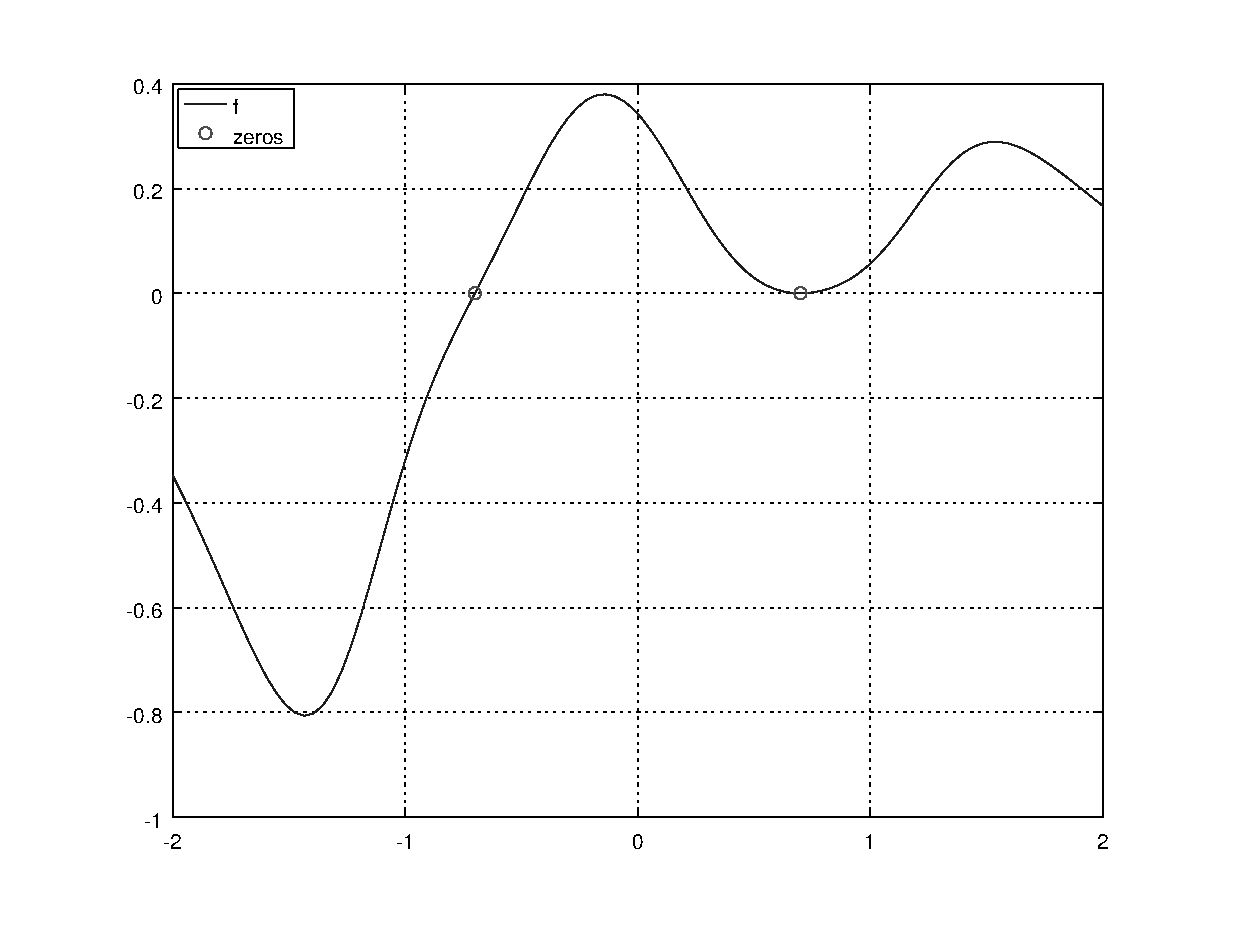
\includegraphics[width=0.8\textwidth]{./cap_eq1d/dados/ex_bis_intro/fig_bis_intro}
  \caption{Esboço da função $f$ do Exemplo~\ref{ex:bis_intro}.}
  \label{fig:bis_intro}
\end{figure}

Observamos que esta função é contínua e que, por exemplo, $f(-2)>0$ e $f(3)<0$, logo $f(-2)\cdot f(3) < 0$ e, de fato, $f$ tem pelo menos um zero\footnote{De fato, $f$ tem três zeros no intervalo $(-2, 3)$.} no intervalo $(-2, 3)$.

\ifisoctave
O esboço do gráfico da função $f$ pode ser feito no \verb+GNU Octave+ com o seguinte \href{https://github.com/phkonzen/notas/blob/master/src/MatematicaNumerica/cap_eq1d/dados/ex_bis_intro/ex_bis_intro.m}{código}:
\verbatiminput{./cap_eq1d/dados/ex_bis_intro/ex_bis_intro.m}
\fi
\end{ex}

Consideremos, então, uma função $f$ contínua tal que $f(a)\cdot f(b) < 0$. O método da bisseção é iterativo, sendo que a primeira aproximação para uma solução de $f(x)=0$ tomada como o ponto médio do intervalo $(a, b)$, i.e.
\begin{equation}
  x^{(1)} = \frac{a^{(1)}+b^{(1)}}{2},
\end{equation}
onde $a^{(1)} = a$ e $b^{(1)} = b$. Daí, se ocorrer $f(x^{(1)})=0$ o problema está resolvido. Caso contrário, $f$ tem pelo menos um zero num dos subintervalos $(a^{(1)}, x^{(1)})$ ou $(x^{(1)}, b^{(1)})$, pois $f(a^{(1)})\cdot f(x^{(1)}) < 0$ ou  $f(x^{(1)})\cdot f(b^{(1)}) < 0$, respectivamente e exclusivamente. No primeiro caso, escolhemos $(a^{(2)}, b^{(2)}) = (a^{(1)}, x^{(1)})$ ou, no segundo caso, tomamos $(a^{(2)}, b^{(2)}) = (x^{(1)}, b^{(1)})$. Então, a segunda aproximação para uma solução é computada como
\begin{equation}
  x^{(2)} = \frac{a^{(2)} + b^{(2)}}{2}.
\end{equation}
Daí, o procedimento se repete até obtermos uma aproximação com a precisão desejada.

\begin{ex}\label{ex:bis_exec}
  Consideremos o problema de encontrar um zero da função
\begin{equation}
  f(x) = \sen^2\left(x+\frac{\pi}{4}\right) - x^3 + \frac{\pi}{4}x^2 + \frac{5\pi^2}{16}x + \frac{3\pi^3}{64}.
\end{equation}
Do esboço de seu gráfico (Figura \ref{fig:bis_intro}) vemos que $f(2)\cdot f(3) \neq 0$ sendo que o zero $x=3\pi/4\approx 2,3562$ de $f$ está no intervalo $(2, 3)$. Então, aplicando o método da bisseção com intervalo inicial $(a^{(1)}, b^{(1)}) = (2, 3)$ e aproximação inicial $x^{(1}) = (a^{(1)}+b^{(1)})/2$, obtemos as aproximações apresentadas na Tabela \ref{tab:bis_exec}.

\begin{table}[h!]
  \centering
  \caption{Resultados referentes ao Exemplo~\ref{ex:bis_exec}.}
  \begin{tabular}{r|rr|r|c}
    k & $a^{(k)}$ & $b^{(k)}$ & $x^{(k)}$ & $f(a^{(k)})\cdot f(x^{(k)})$\\\hline
    1 & $2,0000$ & $3,0000$ & $2,5000$ & -1 \\
    2 & $2,0000$ & $2,5000$ & $2,2500$ &  1 \\
    3 & $2,2500$ & $2,5000$ & $2,3750$ & -1 \\
    4 & $2,2500$ & $2,3750$ & $2,3125$ & 1 \\
    5 & $2,3125$ & $2,3750$ & $2,3438$ & 1 \\
    6 & $2,3438$ & $2,3750$ & $2,3594$ &  -1 \\
    7 & $2,3438$ & $2,3594$ & $2,3516$ & 1 \\
    8 & $2,3516$ & $2,3594$ & $2,3555$ &  1 \\
    9 & $2,3555$ & $2,3594$ & $2,3574$ &  -1 \\
    10 & $2,3555$ & $2,3574$ & $2,3564$ & -1 \\\hline
  \end{tabular}
  \label{tab:bis_exec}
\end{table}

\ifisoctave
A tabela \ref{tab:bis_exec} pode ser obtida no \verb+GNU Octave+ com o seguinte \href{https://github.com/phkonzen/notas/blob/master/src/MatematicaNumerica/cap_eq1d/dados/ex_bis_exec/ex_bis_exec.m}{código}:
\verbatiminput{./cap_eq1d/dados/ex_bis_exec/ex_bis_exec.m}
\fi
\end{ex}

\subsection{Análise de convergência}

Dada uma função estritamente monótona\footnote{Estritamente crescente ou estritamente decrescente.} e contínua $f:[a, b]\to\mathbb{R}$ com $f(a)\cdot f(b) < 0$, temos que o método da bisseção converge para o zero de $f$ no intervalo $(a, b)$. 

De fato, como consequência imediata do \href{https://phkonzen.github.io/notas/AnaliseMatematicaI/cap_continuidade_sec_prop_f_cont.html}{teorema do valor intermediário}, temos que $f$ tem pelo menos um zero no intervalo $(a, b)$. Agora, da hipótese de monotonicidade estrita, temos que $f$ tem um único zero neste intervalo, o qual denotaremos por $x^{*}$.

Da construção das iteradas do método, temos
\begin{align}
  |x^{(k)} - x^{*}| &\leq \frac{b^{(k)}-a^{(k)}}{2}\\
  &\leq \frac{b^{(k-1)}-a^{(k-1)}}{2^2}\\
  &\vdots \\
  &\leq \frac{b^{(1)}-a^{(1)}}{2^k},
\end{align}
donde, temos a seguinte estimativa do erro de truncamento
\begin{equation}\label{eq:bis_est_trunc}
  |x^{(k)} - x^{*}| \leq \frac{b^{(1)}-a^{(1)}}{2^k}.
\end{equation}
E, daí também, segue a convergência do método da bisseção, pois
\begin{equation}
  \lim_{k\to\infty} |x^{(k)}-x^{*}| = \lim_{k\to\infty} \frac{b^{(1)}-a^{(1)}}{2^k} = 0.
\end{equation}

\begin{obs}
  No caso de $f$ não ser estritamente monótona no intervalo $(a, b)$, ainda podemos garantir a convergência do método da bisseção. Isto segue do fato de que após algumas iteradas, digamos $k$ iteradas, a função $f$ terá apenas um zero no intervalo $(a^{(k)}, b^{(k)})$. A partir daí, as estimativas acima podem ser aplicadas.
\end{obs}

\begin{ex}\label{ex:bis_conv}
  No Exemplo \ref{ex:bis_exec} aplicamos o método da bisseção para a função
\begin{equation}
  f(x) = \sen^2\left(x+\frac{\pi}{4}\right) - x^3 + \frac{\pi}{4}x^2 + \frac{5\pi^2}{16}x + \frac{3\pi^3}{64}.
\end{equation}
no intervalo $(2, 3)$. Observando os resultados mostrados na Tabela \ref{tab:bis_exec}, vemos que
\begin{equation}
  |x^{(10)}-x^*| = 2,5\E-4,
\end{equation}
com $x^* = x_1 = 3\pi/4$. Observamos que este resultado é consistente com a estimativa do erro de truncamento \eqref{eq:bis_est_trunc}, da qual temos
\begin{align}
  |x^{(10)} - x^*| &\leq \frac{b^{(1)}-a^{(1)}}{2^{10}}\\
  &= \frac{1}{2^{10}} = 9,8\E-4.
\end{align}
\end{ex}

\begin{obs}(\normalfont{Taxa de convergência.})
  A estimativa de convergência \eqref{eq:bis_est_trunc} também pode ser usada para mostrarmos que, assintoticamente, o método da bisseção tem a seguinte taxa de convergência linear
  \begin{equation}
    \left|x^{(k+1)} - x^{(k)}\right| \lesssim \frac{1}{2}\left|x^{(k)} - x^{(k-1)}\right|^{\pmb{1}}.
  \end{equation}
\end{obs}

\subsection{Zeros múltiplos}

Sejam $f$ uma função suave e $x^*$ um zero de multiplicidade par de $f$. Observamos que o método da bisseção não é diretamente aplicável para aproximar $x^*$. Isto ocorre, pois, neste caso, $x^*$ será um ponto de mínimo ou de máximo local de $f$, não havendo pontos $a$ e $b$ próximos de $x^*$ tal que $f(a)\cdot f(b) < 0$.

Agora, sendo $x^*$ é um zero de multiplicidade $2m$ de $f$, temos que ela admite a seguinte decomposição
\begin{equation}
  f(x) = (x-x^*)^{2m}g(x),
\end{equation}
onde $g$ é uma função suave e $g(x^*)\neq 0$. Daí, a derivada de $f$
\begin{equation}
  f'(x) = 2m(x-x^*)^{2m-1}g(x) + (x-x^*)^{2m}g'(x),
\end{equation}
tem $x^*$ como um zero de multiplicidade $2m-1$ (ímpar) e, desta forma, podemos aplicar o método da bisseção em $f'$ para aproximar $x^*$.

\begin{ex}\label{ex:bis_multpar}
  A função
\begin{equation}
  f(x) = \sen^2\left(x+\frac{\pi}{4}\right) - x^3 + \frac{\pi}{4}x^2 + \frac{5\pi^2}{16}x + \frac{3\pi^3}{64}.
\end{equation}
tem $x=-\pi/4\approx -0,7854$ como um zero de multiplicidade par (veja Figura \ref{fig:bis_intro}). Para aplicarmos o método da bisseção para aproximarmos este zero, primeiramente, derivamos $f$
\begin{equation}
  f'(x) = 2\sin(x+\pi/4)\cos(x+\pi/4) - 3x^2 + \frac{\pi}{2}x + \frac{5\pi^2}{16}.
\end{equation}
O esboço do gráfico de $f'$ (Figura \ref{fig:bis_multpar}) mostra que $f'(-1)\cdot f'(0) < 0$ sendo que no intervalo $(-1, 0)$ $f'$ tem um zero de multiplicidade ímpar. Então, aplicando o método da bisseção a $f'$ no intervalo inicial $(a^{(1)}, b^{(1)}) = (-1, ~0)$, obtemos os resultados apresentados na Tabela~\ref{tab:bis_multpar}. Nesta tabela são apresentados as iteradas até a convergência da solução com precisão de $10^{-3}$.

\begin{figure}[h!]
  \centering
  \includegraphics[width=0.8\textwidth]{./cap_eq1d/dados/ex_bis_multpar/fig_bis_multpar}
  \caption{Esboço do gráfico da $f$ e de sua derivada $f'$ dada no Exemplo \ref{ex:bis_multpar}.}
  \label{fig:bis_multpar}
\end{figure}

\begin{table}[h!]
  \centering
  \caption{Resultados referentes ao Exemplo~\ref{ex:bis_exec}.}
  \begin{tabular}{r|rr|r|c}
    k & $a^{(k)}$ & $b^{(k)}$ & $x^{(k)}$ & $f'(a^{(k)})\cdot f'(x^{(k)})$\\\hline
    1 & $-1,0000\E+0$ & $0,0000\E+0$ & $-5,0000\E-1$ & -1 \\
    2 & $-1,0000\E+0$ & $-5,0000\E-1$ & $-7,5000\E-1$ & -1 \\
    3 & $-1,0000\E+0$ & $-7,5000\E-1$ & $-8,7500\E-1$ & 1 \\
    4 & $-8,7500\E-1$ & $-7,5000\E-1$ & $-8,1250\E-1$ &  1 \\
    5 & $-8,1250\E-1$ & $-7,5000\E-1$ & $-7,8125\E-1$ & -1 \\
    6 & $-8,1250\E-1$ & $-7,8125\E-1$ & $-7,9688\E-1$ & 1 \\
    7 & $-7,9688\E-1$ & $-7,8125\E-1$ & $-7,8906\E-1$ & 1 \\
    8 & $-7,8906\E-1$ & $-7,8125\E-1$ & $-7,8516\E-1$ & -1 \\
    9 & $-7,8906\E-1$ & $-7,8516\E-1$ & $-7,8711\E-1$ & 1 \\
    10 & $-7,8711\E-1$ & $-7,8516\E-1$ & $-7,8613\E-1$ & 1 \\\hline
  \end{tabular}
  \label{tab:bis_multpar}
\end{table}

\ifisoctave
A tabela \ref{tab:bis_multpar} pode ser obtida no \verb+GNU Octave+ com o seguinte \href{https://github.com/phkonzen/notas/blob/master/src/MatematicaNumerica/cap_eq1d/dados/ex_bis_multpar/ex_bis_multpar.m}{código}:
\verbatiminput{./cap_eq1d/dados/ex_bis_multpar/ex_bis_multpar.m}
\fi
\end{ex}

\subsection*{Exercícios}

\begin{exer}\label{exer:bis_1}
  Use o método da bisseção para aproximar um zero de $f(x)=x^3\sen(x)-\cos(x)$, aplicando como intervalo inicial $(a^{(1)}, b^{(1)}) = (0,5, ~1)$ e aproximação inicial $x^{(1)}=(a^{(1)}+b^{(1)})/2$. Faça, então, $6$ iterações de forma a obter a aproximação $x^{(7)}$ e forneça-a com $7$ dígitos significativos por arredondamento.
\end{exer}
\begin{resp}
    \ifisoctave 
  \href{https://github.com/phkonzen/notas/blob/master/src/MatematicaNumerica/cap_eq1d/dados/exer_bis_1/exer_bis_1.m}{Código.} 
  \fi
  $9,179688\times 10^{-1}$
\end{resp}

\begin{exer}\label{exer:bis_est_trunc}
  Considere que o método da bisseção para aproximar um zero de $f(x)=x^3\sen(x)-\cos(x)$, aplicando como intervalo inicial $(a^{(1)}, b^{(1)}) = (0,5, ~1)$ e aproximação inicial $x^{(1)}=(a^{(1)}+b^{(1)})/2$. Use a estimativa de convergência \eqref{eq:bis_est_trunc}
  \begin{equation}
    \left|x^{(k)} - x^{*}\right| \leq \frac{b^{(1)}-a^{(1)}}{2^k},
  \end{equation}
para estimar o número mínimo de iterações $k_{conv}$ necessárias para se obter a solução com exatidão de $10^{-4}$. Então, compute $x^{(k_{conv})}$ e forneça-o com $6$ dígitos significativos por arredondamento.
\end{exer}
\begin{resp}
    \ifisoctave 
  \href{https://github.com/phkonzen/notas/blob/master/src/MatematicaNumerica/cap_eq1d/dados/exer_bis_este_trunc/exer_bis_est_trunc.m}{Código.} 
  \fi
  $9,15833\E-1$
\end{resp}

\begin{exer}\label{exer:bis_multpar}
  Use o método da bisseção para encontrar uma aproximação com precisão de $10^{-4}$ do zero de
  \begin{equation}
    f(x) = (-x^2+1,154x-0,332929)\cos(x) + x^2 - 1,154x + 0,332929
  \end{equation}
no intervalo $(0,55, ~0,65)$. Forneça a aproximação computada com $7$ dígitos significativos por arredondamento.
\end{exer}
\begin{resp}
    \ifisoctave 
  \href{https://github.com/phkonzen/notas/blob/master/src/MatematicaNumerica/cap_eq1d/dados/exer_bis_multpar/exer_bis_multpar.m}{Código.} 
  \fi
  $5,770508\times 10^{-1}$
\end{resp}

\section{Método da falsa posição}\label{cap_eq1d_sec_falsapos}

O método da falsa posição é uma variação do método da bisseção. Dada uma função $f$ contínua, escolhemos um intervalo inicial $(a, b)$ tal que $f(a)\cdot f(b) < 0$ (i.e. $f$ tem sinais trocados nos pontos $a$ e $b$). Então, uma aproximação para o zero de $f$ neste intervalo é computada como o ponto de interseção da reta secante a $f$ pelos pontos $(a, f(a))$ e $(b, f(b))$, i.e.
\begin{equation}
  x = a - \frac{b-a}{f(b)-f(a)}f(a).
\end{equation}
Veja a Figura \ref{fig:falsapos}.

\begin{figure}[h!]
  \centering
  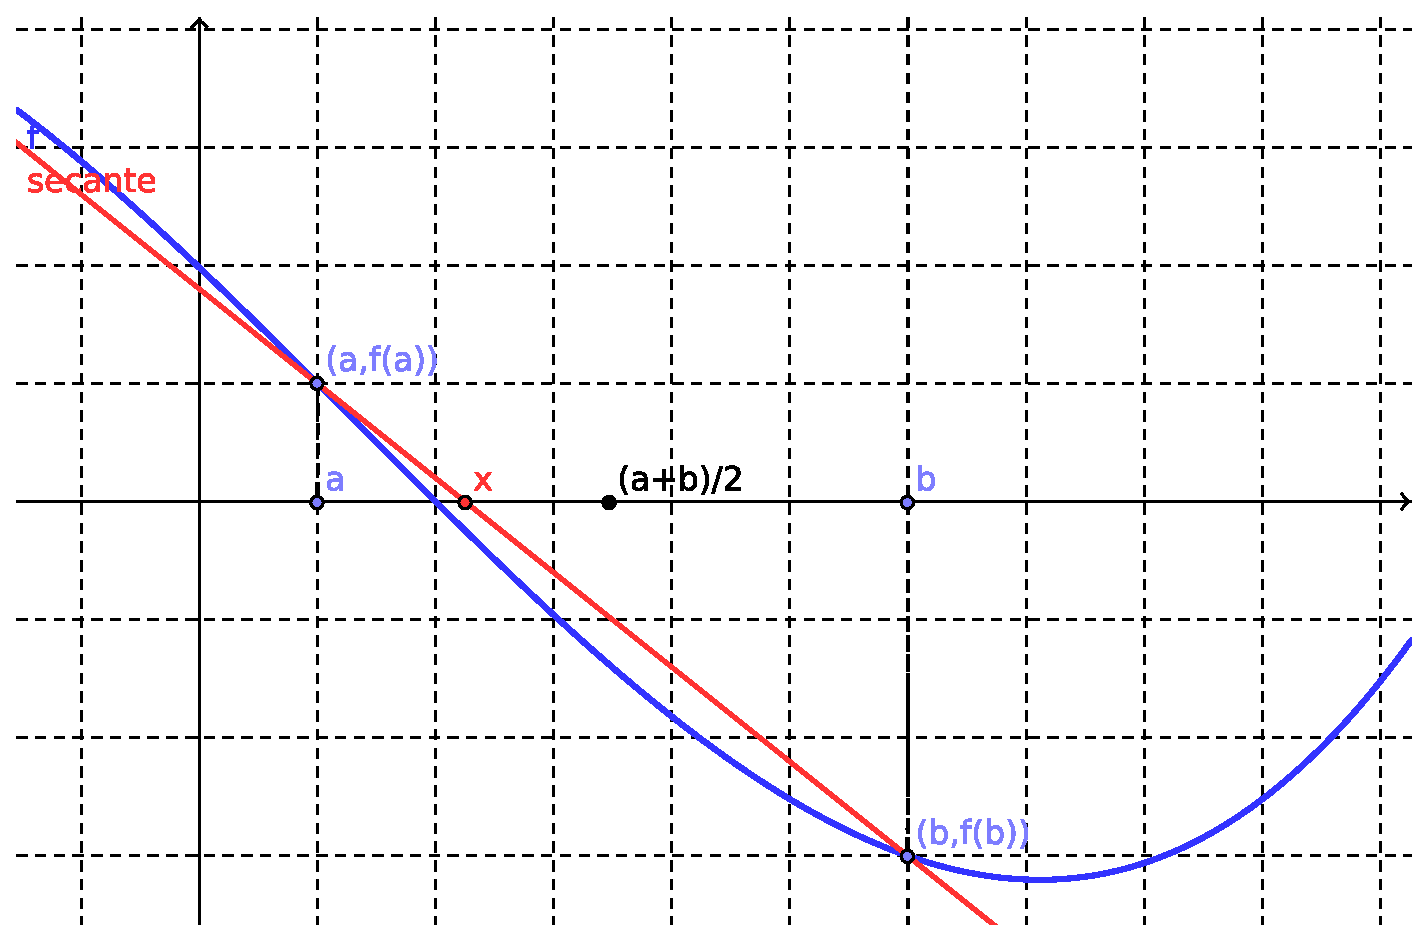
\includegraphics[width=0.7\textwidth]{./cap_eq1d/dados/fig_falsapos/fig_falsapos}
  \caption{Ilustração do método da falsa posição (veja no \href{https://github.com/phkonzen/notas/blob/master/src/MatematicaNumerica/cap_eq1d/dados/fig_falsapos/fig_falsapos.ggb}{Geogebra}).}
  \label{fig:falsapos}
\end{figure}

Mais explicitamente, o método da falsa posição consiste no seguinte procedimento iterativo:
\begin{enumerate}
\item Determinar um intervalo $(a^{(1)}, b^{(1)})$ tal que $f(a^{(1)})\cdot f(b^{(1)}) \neq 0$.
\item Para $k = 1, 2, 3, \cdots, N$:
  \begin{enumerate}[2.1]
  \item $\displaystyle x^{(k)} = a^{(k)} - \frac{b^{(k)}-a^{(k)}}{f(b^{(k)})-f(a^{(k)})}f(a^{(k)})$
  \item Verificar critério de parada.
  \item Se $f(a^{(k)})\cdot f(x^{(k)}) \neq 0$, então $a^{(k+1)}=a^{(k)}$ e $b^{(k+1)}=x^{(k)}$.
  \item Se $f(x^{(k)})\cdot f(b^{(k)}) \neq 0$, então $a^{(k+1)}=x^{(k)}$ e $b^{(k+1)}=b^{(k)}$.
  \end{enumerate}
\end{enumerate}

\begin{ex}\label{ex:falsapos_exec}
  Consideremos o problema de aproximar o zero de
\begin{equation}
  f(x) = \sen^2\left(x+\frac{\pi}{4}\right) - x^3 + \frac{\pi}{4}x^2 + \frac{5\pi^2}{16}x + \frac{3\pi^3}{64}.
\end{equation}
no intervalo $(0, 3)$. A Tabela \ref{tab:falsapos_exec} mostra os resultados obtidos da aplicação do método da falsa posição com intervalo inicial $(a^{(1)}, b^{(1)}) = (2, 3)$. Aqui, o método foi iterado até a convergência com cinco dígitos significativos.

\begin{table}[h!]
  \centering
  \caption{Resultados referentes ao Exemplo~\ref{ex:falsapos_exec}.}
  \begin{tabular}{r|rr|r|c}
    k & $a^{(k)}$ & $b^{(k)}$ & $x^{(k)}$ & $f'(a^{(k)})\cdot f'(x^{(k)})$\\\hline
    1 & $2,0000$ & $3,0000$ & $2,2455$ & 1 \\
    2 & $2,2455$ & $3,0000$ & $2,3240$ &  1 \\
    3 & $2,3240$ & $3,0000$ & $2,3470$ & 1 \\
    4 & $2,3470$ & $3,0000$ & $2,3536$ & 1 \\
    5 & $2,3536$ & $3,0000$ & $2,3555$ & 1 \\
    6 & $2,3555$ & $3,0000$ & $2,3560$ & 1 \\
    7 & $2,3560$ & $3,0000$ & $2,3561$ &  1 \\
    8 & $2,3561$ & $3,0000$ & $2,3562$ & 1 \\
    9 & $2,3562$ & $3,0000$ & $2,3562$ & 1 \\
    10 & $2,3562$ & $3,0000$ & $2,3562$ & 1 \\\hline
  \end{tabular}
  \label{tab:falsapos_exec}
\end{table}

\ifisoctave
A tabela \ref{tab:falsapos_exec} pode ser obtida no \verb+GNU Octave+ com o seguinte \href{https://github.com/phkonzen/notas/blob/master/src/MatematicaNumerica/cap_eq1d/dados/ex_falsapos_exec/ex_falsapos_exec.m}{código}:
\verbatiminput{./cap_eq1d/dados/ex_falsapos_exec/ex_falsapos_exec.m}
\fi
\end{ex}

\subsection*{Exercícios}

\begin{exer}\label{exer:falsapos_1}
  Use o método da falsa posição para aproximar um zero de $f(x)=x^3\sen(x)-\cos(x)$, aplicando como intervalo inicial $(a^{(1)}, b^{(1)}) = (0,5, ~1)$ e aproximação inicial
  \begin{equation}
    x^{(1)} = a^{(1)} - \frac{b^{(1)}-a^{(1)}}{f(b^{(1)})-f(a^{(1)})}f(a^{(1)}).
  \end{equation}
Faça, então, $4$ iterações deste método de forma a obter a aproximação $x^{(5)}$ e forneça-a com $7$ dígitos significativos por arredondamento.
\end{exer}
\begin{resp}
    \ifisoctave 
  \href{https://github.com/phkonzen/notas/blob/master/src/MatematicaNumerica/cap_eq1d/dados/exer_falsapos_1/exer_falsapos_1.m}{Código.} 
  \fi
  $9,158079\times 10^{-1}$
\end{resp}

\begin{exer}\label{exer:falsapos_multpar}
  Use o método da bisseção para encontrar uma aproximação com precisão de $10^{-4}$ do zero de
  \begin{equation}
    f(x) = (-x^2+1,154x-0,332929)\cos(x) + x^2 - 1,154x + 0,332929
  \end{equation}
no intervalo $(0,55, ~0,65)$. Forneça a aproximação computada com $7$ dígitos significativos por arredondamento.
\end{exer}
\begin{resp}
    \ifisoctave 
  \href{https://github.com/phkonzen/notas/blob/master/src/MatematicaNumerica/cap_eq1d/dados/exer_falsapos_multpar/exer_falsapos_multpar.m}{Código.} 
  \fi
  $5,76984\times 10^{-1}$
\end{resp}

\section{Iteração de ponto fixo}\label{cap_eq1d_pfixo}

O ponto fixo de uma função dada $g$ é o ponto $x$ tal que
\begin{equation}
  g(x) = x.
\end{equation}
Geometricamente, pontos fixos são interseções do gráfico da $g$ com a reta $y=x$, veja a Figura \ref{fig:pfixo}.

\begin{figure}[h!]
  \centering
  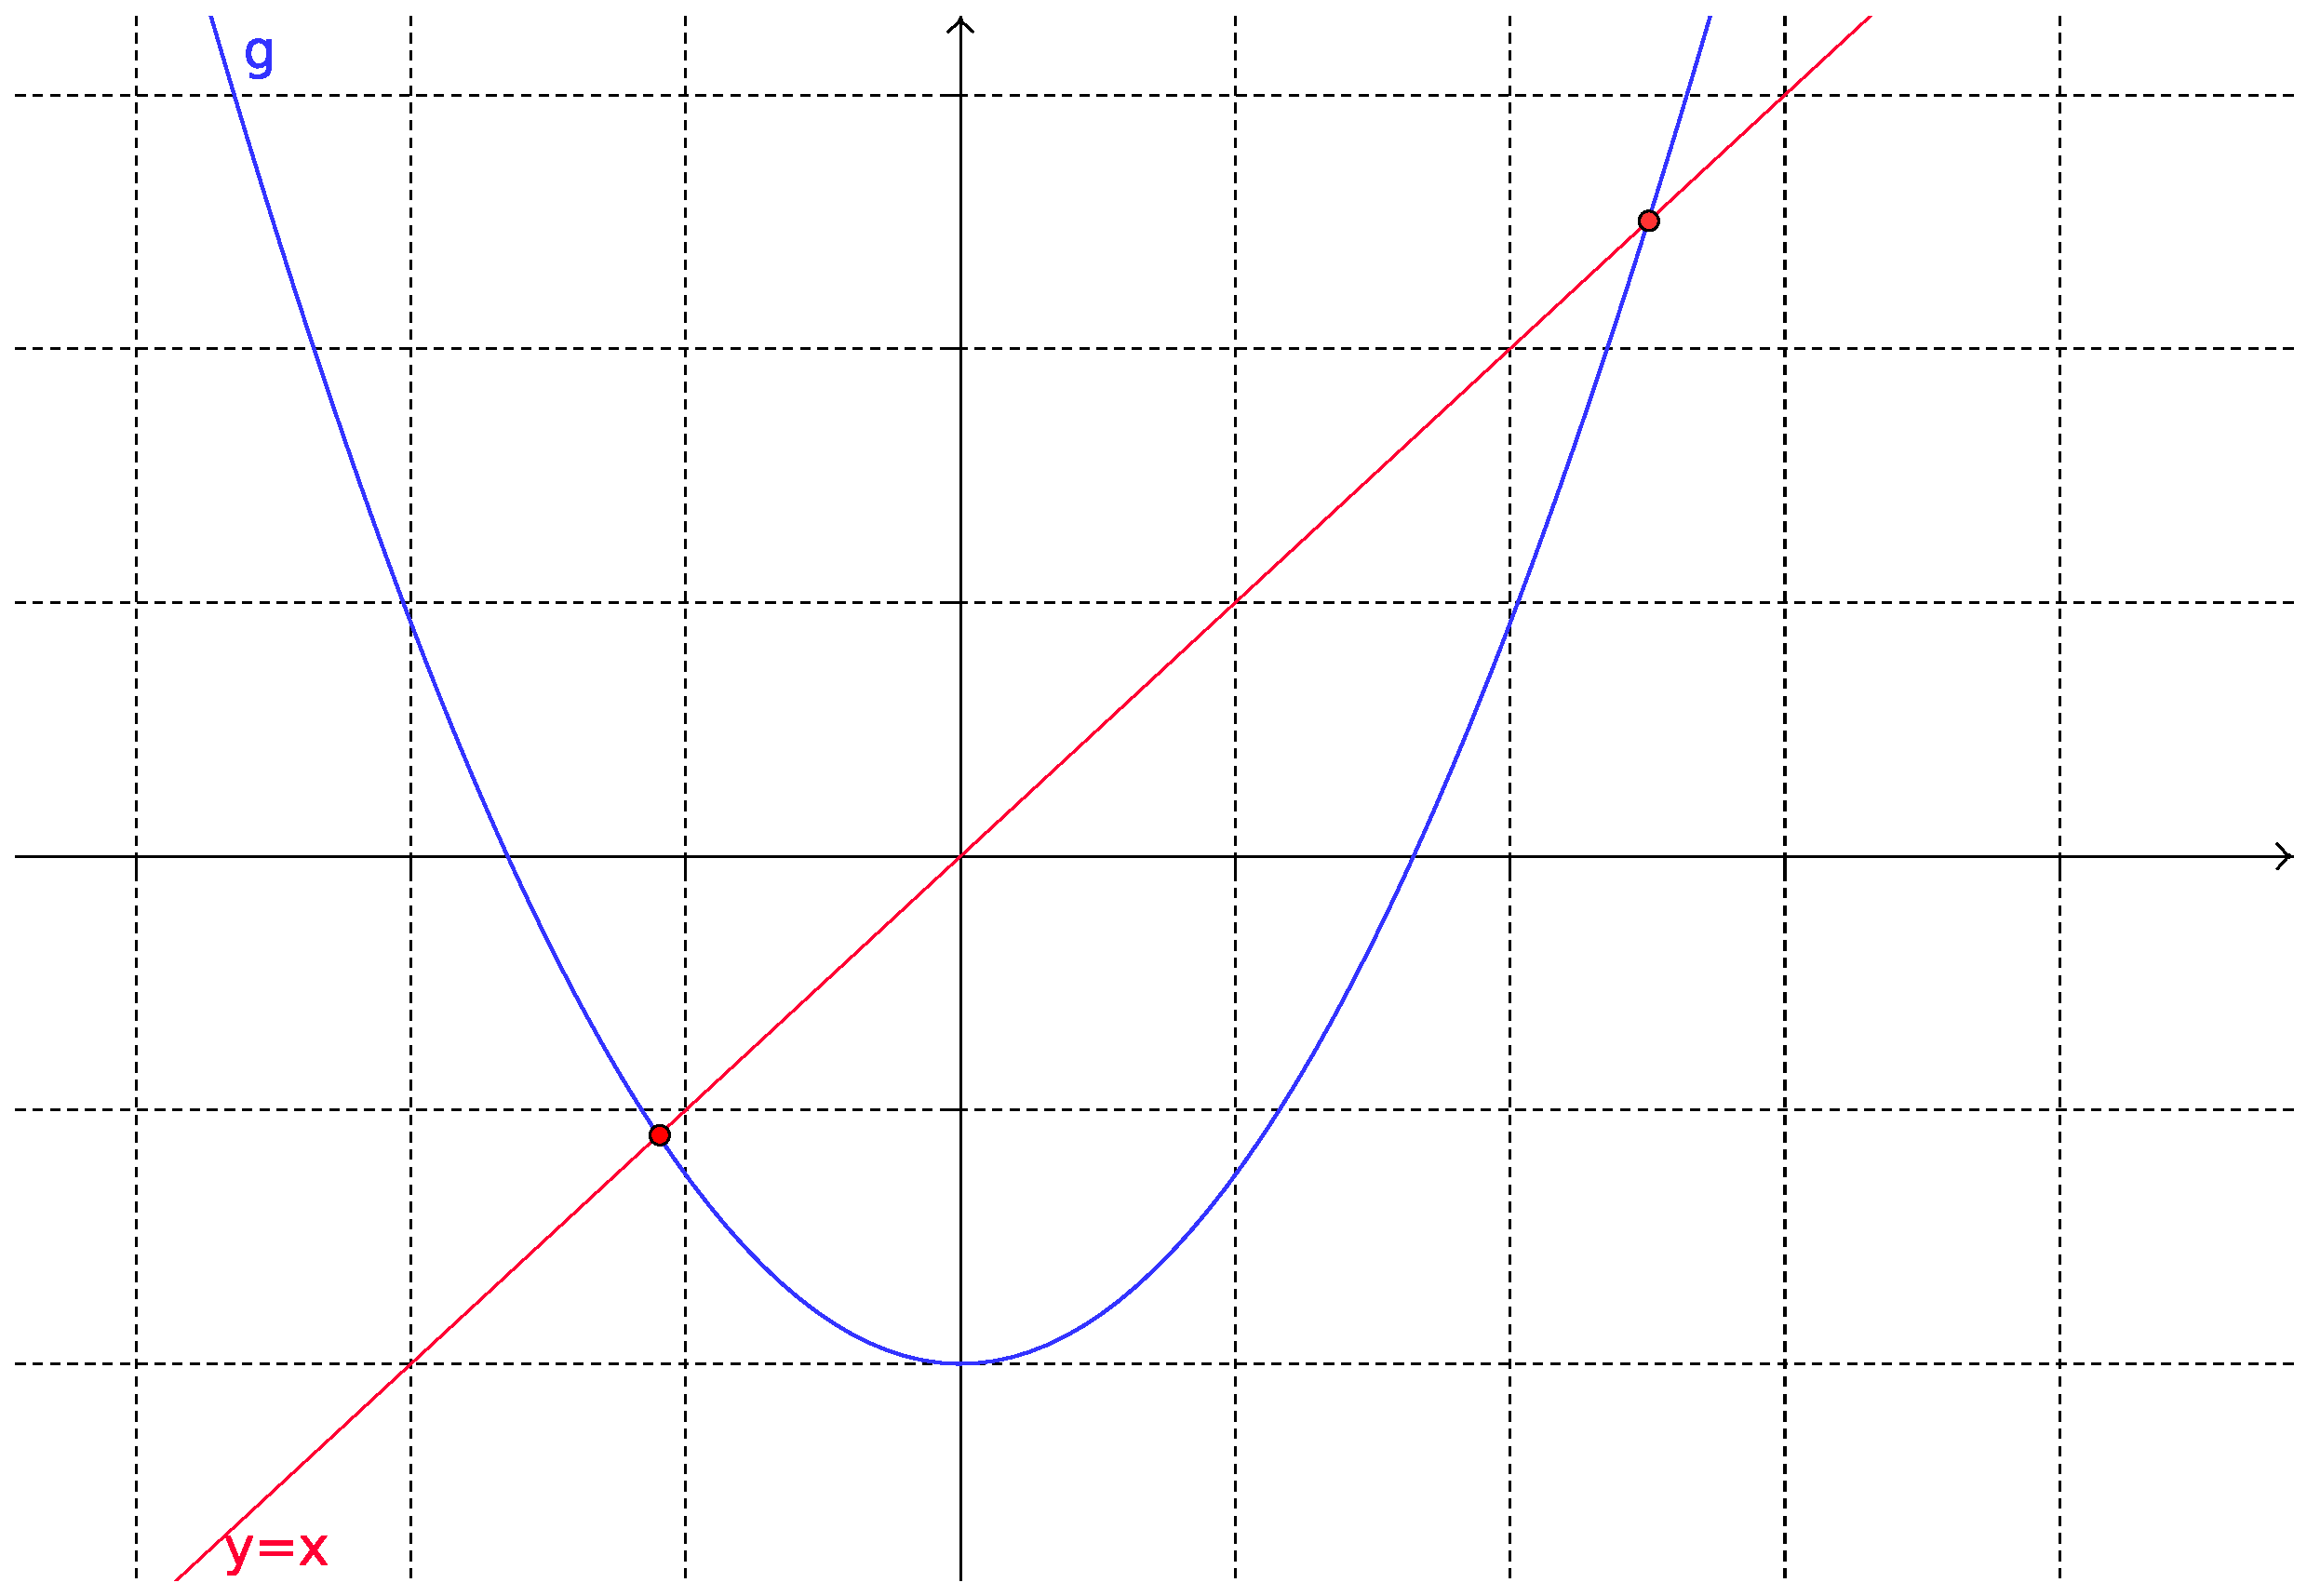
\includegraphics[width=0.8\textwidth]{./cap_eq1d/dados/fig_pfixo/fig_pfixo}
  \caption{Exemplos de pontos fixos (veja no \href{https://github.com/phkonzen/notas/blob/master/src/MatematicaNumerica/cap_eq1d/dados/fig_pfixo/fig_pfixo.ggb}{Geogebra}).}
  \label{fig:pfixo}
\end{figure}

Observamos que toda equação de uma incógnita pode ser reescrita de forma equivalente como um problema de ponto fixo.

\begin{ex}\label{ex:pfixo_intro}
  Consideremos o problema de resolver
  \begin{equation}
    \sen^2\left(x+\frac{\pi}{4}\right) = x^3 - \frac{\pi}{4}x^2 - \frac{5\pi^2}{16}x - \frac{3\pi^3}{64}.
  \end{equation}
Podemos reescrevê-la como o problema de se obter os zeros da seguinte função
\begin{equation}
  f(x) = \sen^2\left(x+\frac{\pi}{4}\right) - x^3 + \frac{\pi}{4}x^2 + \frac{5\pi^2}{16}x + \frac{3\pi^3}{64}.
\end{equation}
Por sua vez, este problema é equivalente aos seguintes problemas de ponto fixo (entre outros):
\begin{align}
  &a)~g_1(x) = \frac{16}{5\pi^2}\left[-\sen^2\left(x+\frac{\pi}{4}\right) + x^3 - \frac{\pi}{4}x^2 - \frac{3\pi^3}{64}\right] = x.\\
  &b)~g_2(x) = \sqrt[3]{\sen^2\left(x+\frac{\pi}{4}\right) + \frac{\pi}{4}x^2 + \frac{5\pi^2}{16}x + \frac{3\pi^3}{64}}
\end{align}
Na Figura \ref{fig:pfixo_intro} podemos observar que os zeros da $f$ (a saber, $x_1=3\pi/4\approx 2,3562$ e $x_2=x_3=-\pi/4\approx -0,78540$) coincidem com os pontos fixos das funções $g_1$ e $g_2$.

\begin{figure}[h!]
  \centering
  \includegraphics[width=0.8\textwidth]{./cap_eq1d/dados/ex_pfixo_intro/fig_pfixo_intro}
  \caption{Esboço da função $f$ do Exemplo~\ref{ex:pfixo_intro}.}
  \label{fig:pfixo_intro}
\end{figure}
\end{ex}

Em muitos casos, é possível obter aproximações de um ponto fixo de uma dada função $g$ pela chamada \emph{iteração de ponto fixo}:
\begin{align}
  x^{(1)} &= \text{aprox. inicial}\\
  x^{(k+1)} &= g(x^{(k)}),\quad k=1, 2, 3, \ldots
\end{align}

\begin{ex}\label{ex:pfixo_testes}
  Observemos que para a função $g_1$ dada no Exemplo \ref{ex:pfixo_intro}, temos as seguintes iterações:
  \begin{align}
    x^{(1)} &= -0,70000,\\
    x^{(2)} &= -0,70959,\\
    x^{(3)} &= -0,71716,\\
    &\vdots \\
    x^{(100)} &= -0,77862,\\
    &\vdots \\
    x^{(1000)} &= -0,78466,\\    
    &\vdots \\
    x^{(20000)} &= -0,78536.
  \end{align}
Ou seja, neste caso as iterações de ponto fixo convergem (lentamente) para o ponto fixo $x=-\pi/4\approx -0,78540$.
\ifisoctave
Veja o \href{https://github.com/phkonzen/notas/blob/master/src/MatematicaNumerica/cap_eq1d/dados/ex_pfixo_testes/ex_g1_t1.m}{código} no \verb+GNU Octave+.
\fi

Agora, se usarmos a iteração de ponto fixo com esta mesma função para aproximar o ponto fixo $x=3\pi/4\approx 2,3562$, obtemos
  \begin{align}
    x^{(1)} &= 2,50000,\\
    x^{(2)} &= 2,9966,\\
    x^{(3)} &= 5,8509,\\
    &\vdots \\
    x^{(8)} &= 4,8921e\times 10^{121}.
  \end{align}
Donde observamos que as iterações divergem rapidamente.

Entretanto, se usarmos a iteração de ponto fixo com a função $f_2$ dada no Exemplo \ref{ex:pfixo_intro}, obtemos
  \begin{align}
    x^{(1)} &= 2,50000,\\
    x^{(2)} &= 2,4155,\\
    x^{(3)} &= 2,3805,\\
    &\vdots \\
    x^{(10)} &= 2,3562.
  \end{align}
A qual, portanto, converge para o ponto fixo esperado.
\end{ex}

Este último exemplo (Exemplo \ref{ex:pfixo_testes}) mostra que a iteração do ponto fixo nem sempre é convergente. Antes de vermos condições suficientes para a convergência, vejamos sua interpretação geométrica.

\subsection{Interpretação geométrica}

A Figura \ref{fig:pfixo_interp} apresenta o caso de uma iteração de ponto fixo convergente. As iterações iniciam-se no ponto $x^{(1)}$ e seguem para $x^{(2)} = g(x^{(1)})$ e $x^{(3)} = g(x^{(2)})$.

\begin{figure}[h!]
  \centering
  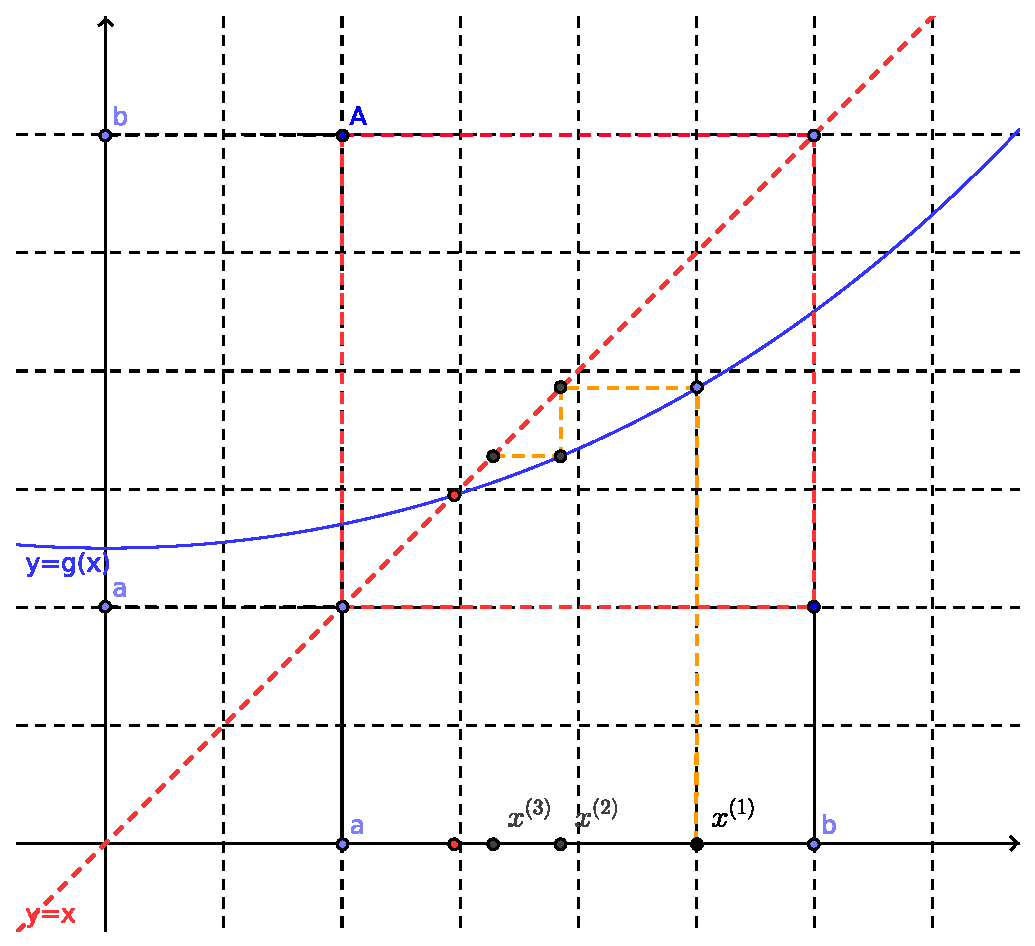
\includegraphics[width=0.8\textwidth]{./cap_eq1d/dados/fig_pfixo_interp/fig_pfixo_interp}
  \caption{Interpretação geométrica da iteração de ponto fixo.}
  \label{fig:pfixo_interp}
\end{figure}

\subsection{Análise de convergência}

O seguinte teorema nos fornece condições suficientes para a convergência das iterações de ponto fixo.

\begin{teo}(\normalfont{Teorema do ponto fixo})\label{teo:pfixo}
  Seja uma dada função $g$ continuamente diferenciável satisfazendo
  \begin{enumerate}[a)]
  \item $g([a, b]) \subset [a, b]$,
  \item $|g'(x)|<K<1$ para todo $x\in [a, b]$.
  \end{enumerate}
Então, $g$ tem um único ponto fixo $x^*\in [a, b]$ e as iterações $x^{(k+1)}=x^{(k)}$, $k=1, 2, 3, \ldots$, convergem para $x^*$, para qualquer escolha de $x^{(1)}\in [a, b]$.
\end{teo}
\begin{dem}
  Da hipótese b), temos que $g$ é uma contração com
  \begin{equation}
    |g(x) - g(y)| < K\cdot |x - y|,~\forall x,y\in [a, b].
  \end{equation}
Com isso, da hipótese a) e tomando $x^{(1)}\in [a, b]$, temos
\begin{align}
  |x^{(k+1)} - x^{(k)}| &= |g(x^{(k)}) - g(x^{(k-1)})|\\
  &\leq K |x^{(k)} - x^{(k-1)}|\\
  &\vdots \\
  &\leq K^{k-1}|x^{(2)}-x^{(1)}|,
\end{align}
para todo $k=2, 3, \ldots$. Como $K<1$, temos $|x^{(k+1)}-x^{(k)}|\to 0$ quando $k\to\infty$ e, portanto, $x^{(k)}$ converge para algum $x^*\in [a, b]$.

De fato, $x^*$ é ponto fixo de $g$, pois da continuidade da $g$, temos
\begin{equation}
  x^* = \lim_{k\to\infty} x^{(k+1)} = \lim_{k\to\infty} g(x^{(k)}) = g(x^*).
\end{equation}

Por fim, $x^*$ é único, pois assumindo a existência de outro ponto fixo $x^{**}\neq x^*$ teríamos
\begin{equation}
  |x^* - x^{**}| = |g(x^*) - g(x^{**})| < K|x^* - x^{**}|.
\end{equation}
\end{dem}

Agora, dado um problema de encontrar um zero de uma dada função $f$, i.e. $f(x)=0$, podemos construir uma função $g$ para a iteração de ponto fixo associada da seguinte forma:
\begin{align}
  f(x) = 0 &\Leftrightarrow \underbrace{x - \alpha f(x)}_{g(x)} = x,
\end{align}
com $\alpha\in\mathbb{R}$ escolhido de forma a satisfazer as hipóteses do teorema do ponto fixo (Teorema \ref{teo:pfixo}).

\begin{ex}\label{ex:pfixo_exec}
  Retornamos ao problema de encontrar o zero da função
  \begin{equation}
    f(x) = \sen^2\left(x+\frac{\pi}{4}\right) - x^3 + \frac{\pi}{4}x^2 + \frac{5\pi^2}{16}x + \frac{3\pi^3}{64}.
  \end{equation}
  no intervalo $[2,3]$. Para construir uma função $g$ para a iteração de ponto fixo neste intervalo, podemos tomar
  \begin{equation}
    g(x) = x - \alpha f(x),
  \end{equation}
com $\alpha = -0,1$. A Figura \ref{fig:ex_pfixo_exec} mostra esboços dos gráficos de $g$ e $|g'|$ no intervalos $[2, 3]$ e podemos observar que esta escolha de $\alpha$ faz com que a $g$ satisfaça o teorema do ponto fixo.

\begin{figure}[h!]
  \centering
  \includegraphics[width=0.8\textwidth]{./cap_eq1d/dados/ex_pfixo_exec/fig_ex_pfixo_exec}
  \caption{Esboço dos gráficos de $g$ e $|g'|$ discutidas no Exemplo \ref{ex:pfixo_exec}.}
  \label{fig:ex_pfixo_exec}
\end{figure}

Então, fazendo as iterações de ponto fixo com aproximação inicial $x^{(1)}=2,6$, obtemos os resultados apresentados na Tabela \ref{tab:ex_pfixo_exec}.

\begin{table}[h!]
  \centering
  \begin{tabular}{r|cc}
    $k$ & $x^{(k)}$ & $|x^{(k)}-x^{(k-1)}|$ \\\hline
    1 & $2,6000$ & -x-\\
    2 & $2,3264$ & $2,7\E-1$ \\
    3 & $2,3553$ & $2,9\E-2$ \\
    4 & $2,3562$ & $8,4\E-4$ \\
    5 & $2,3562$ & $1,1\E-5$ \\\hline
  \end{tabular}
  \caption{Resultados referentes ao Exemplo \ref{ex:pfixo_exec}.}
  \label{tab:ex_pfixo_exec}
\end{table}

\ifisoctave
Os resultados apresentados na Tabela \ref{tab:ex_pfixo_exec} podem ser computados no \verb+GNU Octave+ com o seguinte código:
\verbatiminput{./cap_eq1d/dados/ex_pfixo_exec/ex_pfixo_exec.m}
\fi
\end{ex}

\begin{obs}(\normalfont{Taxa de convergência})
  A iteração de ponto fixo tem taxa de convergência linear
  \begin{equation}
    |x^{(k+1)} - x^{(k)}| < K|x^{(k)} - x^{(k-1)}|^{\pmb{1}},
  \end{equation}
onde $K > 0$ é a constante dada na hipótese $b)$ do teorema do ponto fixo (Teorema \ref{teo:pfixo}). Além disso, isso mostra que quanto menor o valor da constante $K$, mais rápida será a convergência das iterações de ponto fixo.
\end{obs}

\subsection*{Exercícios}

\begin{exer}\label{exer:pfixo_1}
  Considere o problema de computar uma aproximação do zero de $f(x)=x-\cos(x)$. Resolva-o aplicando a iteração de ponto fixo para a função auxiliar
  \begin{equation}
    g(x) = x - \alpha f(x),
  \end{equation}
restrita ao intervalo $[a, b] = [0.5, 1]$ com aproximação inicial $x^{(1)}=(a+b)/2$. Escolha o melhor valor de $\alpha$ entre os seguintes:
\begin{enumerate}
\item $\alpha = 1$
\item $\alpha = 0,5$
\item $\alpha = -0,5$
\item $\alpha = 0,6$
\end{enumerate}
Então, compute uma aproximação do zero de $f$ com $5$ dígitos significativos de precisão.
\end{exer}
\begin{resp}
  \ifisoctave 
  \href{https://github.com/phkonzen/notas/blob/master/src/MatematicaNumerica/cap_eq1d/dados/exer_pfixo_1/exer_pfixo_1.m}{Código.} 
  \fi
  $8,2413\times 10^{-1}$
\end{resp}

\section{Método de Steffensen}\label{cap_eq1d_sec_Steffensen}

O método de Steffensen\footnote{Johan Frederik Steffensen, matemático e estatístico dinamarquês, 1873 - 1961. Fonte: \href{https://en.wikipedia.org/wiki/Johan_Frederik_Steffensen}{Wikipedia}.} é uma aplicação do método de aceleração de convergência $\Delta^2$ de Aitken\footnote{Alexander Aitken, matemático neozelandês, 1895 - 1967. Fonte: \href{https://en.wikipedia.org/wiki/Alexander_Aitken}{Wikipedia}.} à iteração de ponto fixo.

\subsection{Acelerador $\Delta^2$ de Aitken}

Seja dada uma sequência $(x^{(k)})_{k=1}^\infty$ monotonicamente convergente para $x^*$. Assumamos que $k$ seja suficientemente grande tal que
\begin{equation}
  \frac{x^{(k+1)}-x^*}{x^{(k)}-x^*} \approx \frac{x^{(k+2)}-x^*}{x^{(k+1)}-x^*}.
\end{equation}
Então, isolando $x^*$ obtemos
\begin{equation}
  x^* \approx \frac{x^{(k)}x^{(k+2)}-(x^{(k+1)})^2}{x^{(k)}-2x^{(k+1)}+x^{(k+2)}}.
\end{equation}
Ainda, somando e subtraindo $(x^{(k)})^2$ e $2x^{(k)}x^{(k+1)}$ no numerador acima e rearranjando os termos, obtemos
\begin{equation}
  x^* \approx x^{(k)} - \frac{(x^{(k+1)}-x^{(k)})^2}{x^{(k+2)}-2x^{(k+1)}+x^{(k)}}.
\end{equation}

O observado acima, nos motiva a introduzir o acelerador $\Delta^2$ de Aitken
\begin{equation}
  \Delta^2\{x^{(k)},x^{(k+1)},x^{(k+2)}\} := x^{(k)} - \frac{(x^{(k+1)}-x^{(k)})^2}{x^{(k+2)}-2x^{(k+1)}+x^{(k)}}.
\end{equation}


\begin{ex}\label{ex:Aitken}
  Consideremos o problema de encontrar o zero da função
  \begin{equation}
    f(x) = \sen^2\left(x+\frac{\pi}{4}\right) - x^3 + \frac{\pi}{4}x^2 + \frac{5\pi^2}{16}x + \frac{3\pi^3}{64}.
  \end{equation}
  no intervalo $[2,3]$. Para tanto, podemos aplicar a iteração de ponto fixo dada por
  \begin{equation}
    x^{(k+1)} = g(x^{(k)}) := x^{(k)} - \alpha f(x^{(k)}),\quad k=1,2,\ldots,
  \end{equation}
com $\alpha=-0,05$ e $x^{(1)}=2,6$. Na Tabela \ref{tab:ex_Aitken} temos os valores das iteradas $x^{(k)}$ e das correções $\Delta^2 = \Delta^2\{x^{(k)},x^{(k+1)},x^{(k+2)}\}$ de Aitken. Neste caso, a aceleração de convergência é notável.

\begin{table}[h!]
  \centering
  \begin{tabular}{r|cc}
    $k$ & $x^{(k)}$ & $\Delta^2$ \\\hline
    1 & $2,6000$ & -x- \\
    2 & $2,4632$ & -x- \\
    3 & $2,4073$ & $2,3687$ \\
    4 & $2,3814$ & $2,3590$ \\
    5 & $2,3688$ & $2,3569$ \\
    6 & $2,3625$ & $2,3564$ \\
    7 & $2,3594$ & $2,3562$ \\
    8 & $2,3578$ & $2,3562$ \\\hline
  \end{tabular}
  \caption{Resultados referentes ao Exemplo \ref{ex:Aitken}.}
  \label{tab:ex_Aitken}
\end{table}

\ifisoctave
Os resultados apresentados na Tabela \ref{tab:ex_Aitken} podem ser computados no \verb+GNU Octave+ com o seguinte \href{https://github.com/phkonzen/notas/blob/master/src/MatematicaNumerica/cap_eq1d/dados/ex_Aitken/ex_Aitken.m}{código}:
\verbatiminput{./cap_eq1d/dados/ex_Aitken/ex_Aitken.m}
\fi
\end{ex}

\subsection{Algoritmo de Steffensen}

O método de Steffensen consiste em aplicar o acelerador $\Delta^2$ de Aitken à iteração de ponto fixo. Mais especificamente, sejam uma aproximação inicial $x^{(1)}$ e uma iteração de ponto fixo
\begin{equation}
  x^{(k+1)} = g(x^{(k)}),\quad k=1,2,\ldots.
\end{equation}
O algoritmo de Steffensen pode ser descrito como segue:
\begin{enumerate}
\item Fazemos $x = x^{(1)}$.
\item Para $k=1,2,3,\dotsc, N-1$:
  \begin{enumerate}
  \item Computamos $x_1 = g(x^{(k)})$.
  \item Computamos $x_2 = g(x_1)$.
  \item Computamos $x^{(k+1)} = \Delta^2\{x^{(k)},x_1,x_2\}$
  \item Verificamos o critério de parada.
  \end{enumerate}
\end{enumerate}


\begin{ex}\label{ex:Steffensen_exec}
  Retornemos ao exemplo anterior (Exemplo \ref{ex:Aitken}. Na Tabela \ref{tab:ex_Steffensen_exec} temos os valores das iteradas de Steffensen $x^{(k)}$ e do indicador de convergência $|x^{(k)}-x^{(k-1)}|$. Observe que os resultados são compatíveis com aqueles obtidos no último exemplo.

\begin{table}[h!]
  \centering
  \begin{tabular}{r|cc}
    $k$ & $x^{(k)}$ & $|x^{(k)}-x^{(k-1)}|$ \\\hline
    1 & $2,6000$ & -x- \\
    2 & $2,3687$ & $2,3\E-1$ \\
    3 & $2.3562$ & $1,2\E-2$ \\
    4 & $2,3562$ & $4,2\E-5$ \\\hline
  \end{tabular}
  \caption{Resultados referentes ao Exemplo \ref{ex:Steffensen_exec}.}
  \label{tab:ex_Steffensen_exec}
\end{table}

\ifisoctave
Os resultados apresentados na Tabela \ref{tab:ex_Steffensen_exec} podem ser computados no \verb+GNU Octave+ com o seguinte \href{https://github.com/phkonzen/notas/blob/master/src/MatematicaNumerica/cap_eq1d/dados/ex_Steffensen_exec/ex_Steffensen_exec.m}{código}:
\verbatiminput{./cap_eq1d/dados/ex_Steffensen_exec/ex_Steffensen_exec.m}
\fi
\end{ex}

\subsection*{Exercícios}

\begin{exer}\label{exer:Steffensen_1}
  Use o método de Steffensen para obter uma aproximação do zero de $f(x)=x^3\sen(x)-\cos(x)$ no intervalo $[0,5, 1]$ com precisão de $10^{-6}$.
\end{exer}
\begin{resp}
    \ifisoctave 
    \href{https://github.com/phkonzen/notas/blob/master/src/MatematicaNumerica/cap_eq1d/dados/exer_Steffensen_1/exer_Steffensen_1.m}{Código.} 
    \fi
    $9,15811\times 10^{-1}$
\end{resp}

\section{Método de Newton}\label{cap_mef1d_sec_newton}

Seja $x^*$ um zero de uma dada função $f$, i.e. $f(x^*)=0$. Usando de expansão em polinômio de Taylor da $f$ em um dado ponto $\tilde{x}$, temos
\begin{equation}
  f(x^*) = f(\tilde{x}) + f'(\tilde{x})(x^*-\tilde{x}) + O((x^*-\tilde{x})^2).
\end{equation}
Como $f(x^*)=0$, temos
\begin{equation}
  x^* + O((x^*-\tilde{x})^2) = \tilde{x} - \frac{f(\tilde{x})}{f'(\tilde{x})}.
\end{equation}
Esta última expressão nos indica que dada uma aproximação $\tilde{x}$ do zero de $f$ a expressão
\begin{equation}
  \tilde{x} - \frac{f(\tilde{x})}{f'(\tilde{x})},
\end{equation}
aproxima $x^*$ com um erro da ordem de $(x^*-\tilde{x})^2$.

Estes observações nos levam a \emph{iteração de Newton}\footnote{Sir Isaac Newton, matemático e físico inglês, 1642 - 1726/27. Fonte: \href{https://en.wikipedia.org/wiki/Isaac_Newton}{Wikipedia}.}\index{iteração de!Newton}
\begin{align}
  x^{(1)} &= \text{aprox. inicial},\\
  x^{(k+1)} &= x^{(k)} - \frac{f(x^{(k)})}{f'(x^{(k)})},\label{eq:Newton_iteracao}
\end{align}
com $k=1, 2, \ldots$.

\begin{ex}\label{ex:Newton_exec}
  Retornamos ao problema de encontrar o zero da função
  \begin{equation}
    f(x) = \sen^2\left(x+\frac{\pi}{4}\right) - x^3 + \frac{\pi}{4}x^2 + \frac{5\pi^2}{16}x + \frac{3\pi^3}{64}.
  \end{equation}
  no intervalo $[2,3]$. Então, fazendo as iterações de Newton com aproximação inicial $x^{(1)}=2,6$, obtemos os resultados apresentados na Tabela \ref{tab:ex_Newton_exec}.

\begin{table}[h!]
  \centering
  \begin{tabular}{r|cc}
    $k$ & $x^{(k)}$ & $|x^{(k)}-x^{(k-1)}|$ \\\hline
    1 & $2,6000$ & -x-\\
    2 & $2,3836$ & $2,2\E-1$ \\
    3 & $2,3566$ & $2,7\E-2$ \\
    4 & $2,3562$ & $3,9\E-4$ \\
    5 & $2,3562$ & $8,3\E-8$ \\\hline
  \end{tabular}
  \caption{Resultados referentes ao Exemplo \ref{ex:Newton_exec}.}
  \label{tab:ex_Newton_exec}
\end{table}

\ifisoctave
Os resultados apresentados na Tabela \ref{tab:ex_Newton_exec} podem ser computados no \verb+GNU Octave+ com o seguinte \href{https://github.com/phkonzen/notas/blob/master/src/MatematicaNumerica/cap_eq1d/dados/ex_Newton_exec/ex_Newton_exec.m}{código}:
\verbatiminput{./cap_eq1d/dados/ex_Newton_exec/ex_Newton_exec.m}
\fi
\end{ex}

\begin{obs}
  O método de Newton é uma iteração de ponto fixo ótima. Do Teorema do ponto fixo (Teorema \ref{teo:pfixo}), uma iteração de ponto fixo
  \begin{equation}\label{eq:Newton_pfixo}
    x^{k+1} = g(x^{(k)}) := x^{(k)} -\alpha f(x)
  \end{equation}
tem taxa de convergência\footnote{Supondo as demais hipóteses do Teorema \ref{teo:pfixo}.}
\begin{equation}
  |x^{(k+1)}-x^{(k)}| \leq K |x^{(k)}-x^{(k-1)}|,
\end{equation}
com $K$ tal que $|g'(x)|=|1 - \alpha f'(x)|<K<1$. Isto nos indica que a melhor escolha para $\alpha$ é
\begin{equation}
  \alpha = \frac{1}{f'(x)},
\end{equation}
de forma que \eqref{eq:Newton_pfixo} coincide com a iteração de \eqref{eq:Newton_iteracao}.
\end{obs}


\subsection{Interpretação geométrica}

Dada uma aproximação $x^{(k)}$ de um zero de uma dada função $f$, a iteração de Newton fornece uma nova aproximação $x^{(k+1)}$ com
\begin{equation}
  x^{(k+1)} = x^{(k)} - \frac{f(x^{(k)})}{f'(x^{(k)})}.
\end{equation}
Subtraindo $x^{(k+1)}$ e multiplicando por $-f'(x^{(k)})$, obtemos
\begin{equation}\label{eq:Newton_geointerp}
  0 = f'(x^{(k)})(x^{(k+1)}-x^{(k)}) + f(x^{(k)}),
\end{equation}
Observemos que o lado direito desta última equação corresponde a expressão da reta tangente ao gráfico de $f$ pelo ponto $(x^{(k)}, f(x^{(k)}))$, avaliada em $x^{(k+1)}$. Mais precisamente, a equação desta reta tangente é
\begin{equation}
  y = f'(x^{(k)})(x-x^{(k)}) + f(x^{(k)})
\end{equation}
e a equação \eqref{eq:Newton_geointerp} nos informa que em $x=x^{(k+1)}$ a reta tangente cruza o eixo $x$.

\begin{figure}[h!]
  \centering
  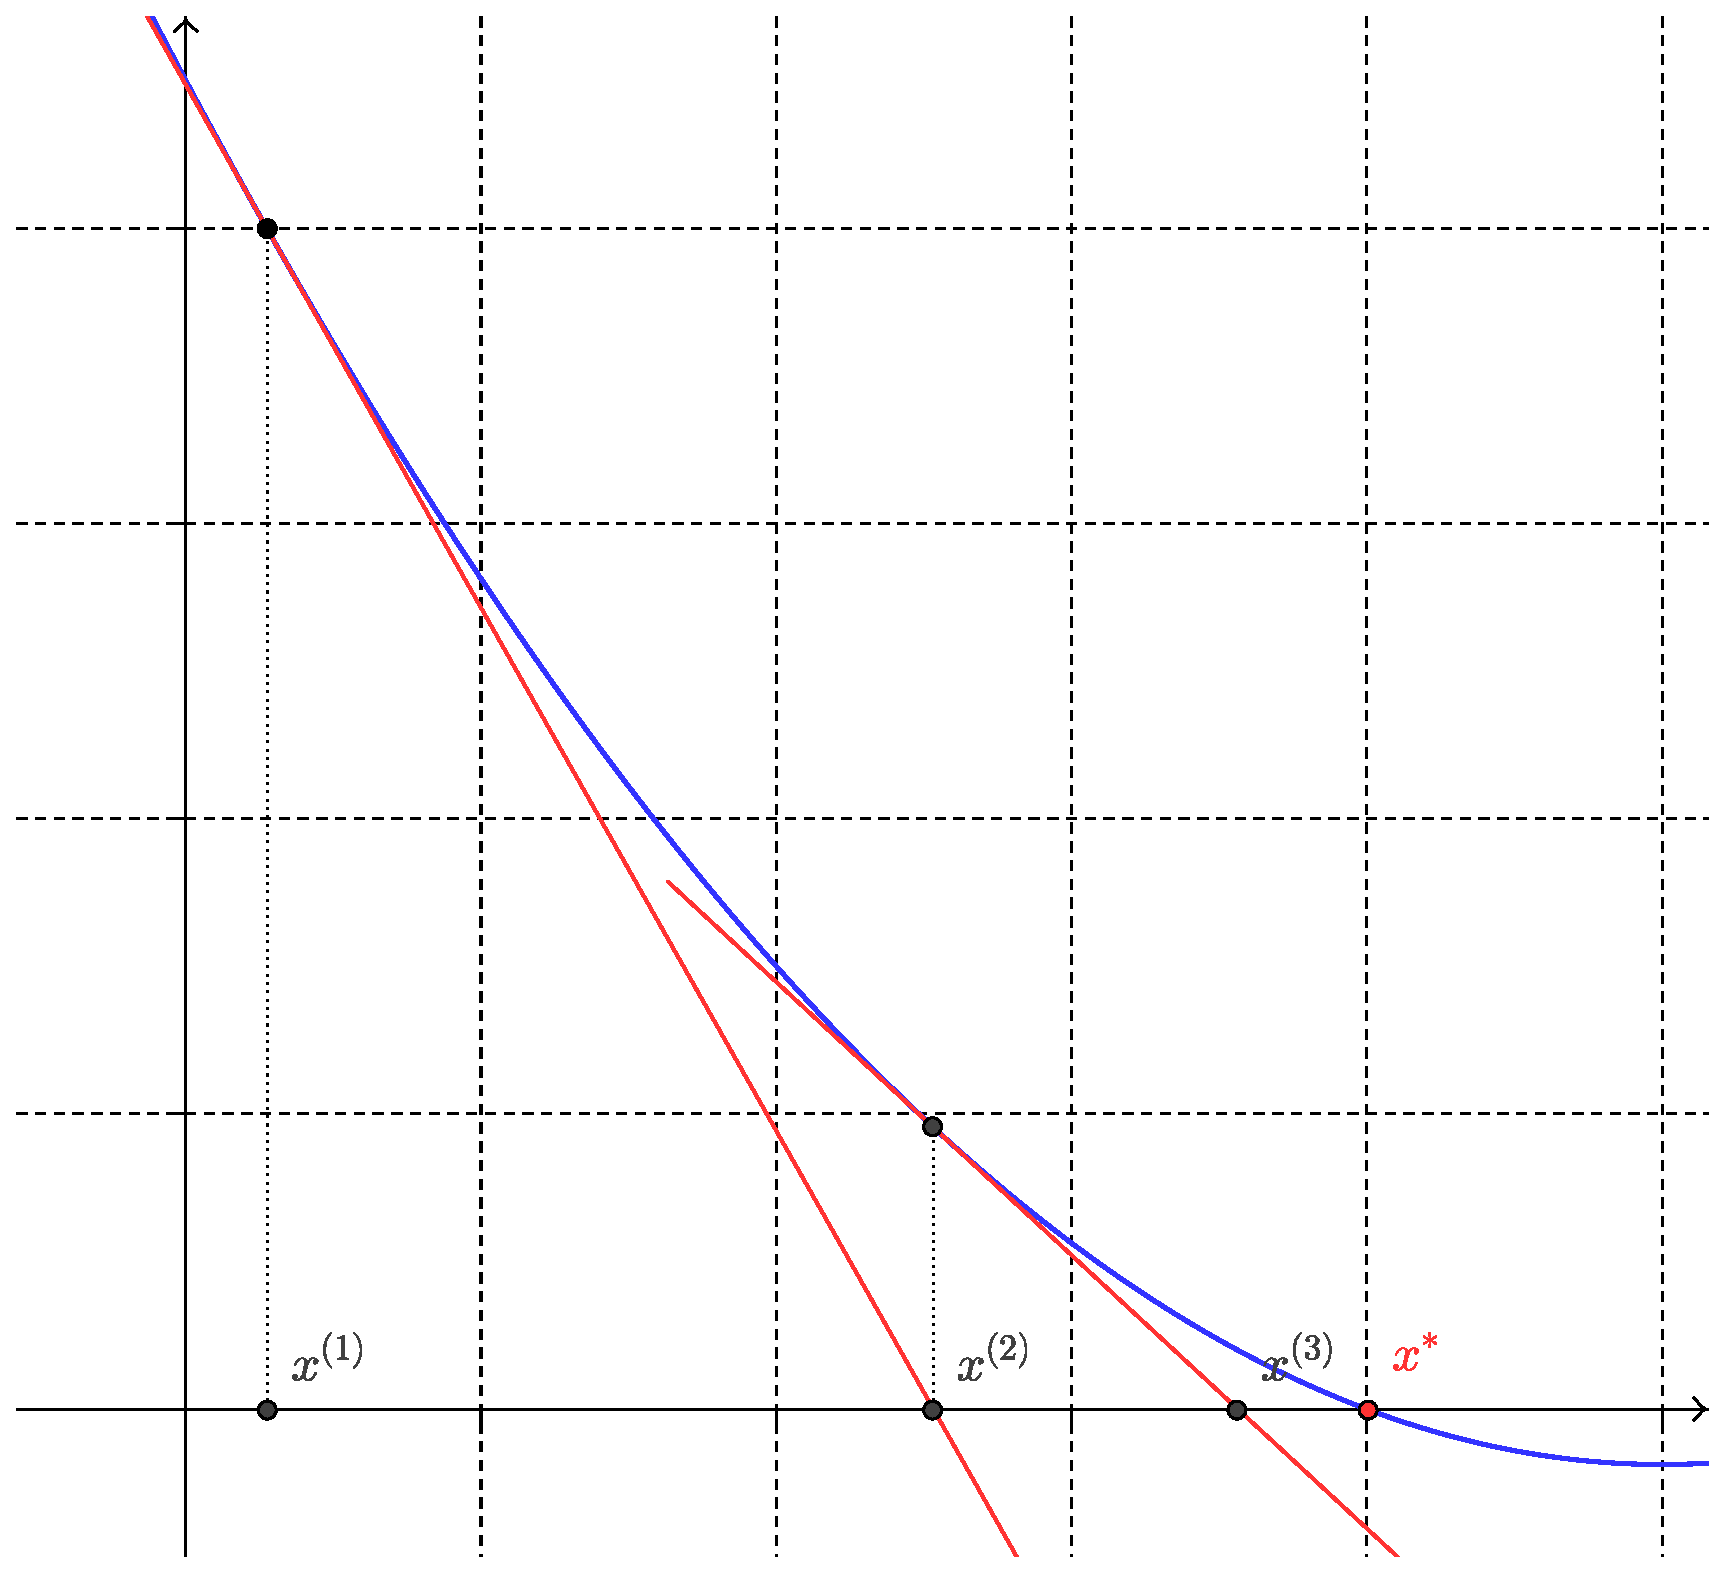
\includegraphics[width=0.8\textwidth]{./cap_eq1d/dados/fig_Newton_geointerp/fig_Newton_geointerp}
  \caption{Interpretação geométrica das iterações de Newton. Veja no \href{https://github.com/phkonzen/notas/blob/master/src/MatematicaNumerica/cap_eq1d/dados/fig_Newton_geointerp/fig_Newton_geointerp.ggb}{Geogebra}.}
  \label{fig:Newton_geointerp}
\end{figure}


Destas observações, concluímos que a iterada $x^{(k+1)}$ do método de Newton corresponde ao ponto de interseção da reta tangente ao gráfico da $f$ pelo ponto $(x^{k}, f(x^{k}))$. Veja a Figura \ref{fig:Newton_geointerp}.

\begin{ex}\label{ex:Newton_init}
  Consideremos que o método de Newton seja usado para aproximarmos o zero de
  \begin{equation}
    f(x) = (x-1)e^{-x^2}.
  \end{equation}
Observemos que esta função tem $x=1$ como seu único zero. Agora, se escolhermos $x^{(1)} = 0,5$ as iterações de Newton convergem para este zero, mas, se escolhermos $x^{(1)}=1,5$ não (veja a Tabela \ref{tab:ex_Newton_init}).

\begin{table}[h!]
  \centering
  \begin{tabular}{r|cc}
    $k$ & $x^{(k)}$ & $x^{(k+1)}$ \\\hline
    1 & $5,0000\E-1$ & $1,5000\E+0$ \\
    2 & $8,3333\E-1$ & $2,5000\E+0$ \\
    3 & $9,6377\E-1$ & $2,7308\E+0$ \\
    4 & $9,9763\E-1$ & $2,9355\E+0$ \\
    5 & $9,9999\E-1$ & $3,1223\E+0$ \\
    6 & $1,0000\E+0$ & $3,2955\E+0$ \\
    7 & $1,0000\E+0$ & $3,4580\E+0$ \\\hline    
  \end{tabular}
  \caption{Resultados referentes ao Exemplo \ref{ex:Newton_init}}
  \label{tab:ex_Newton_init}
\end{table}

  \begin{figure}[h!]
    \centering
    \includegraphics[width=0.8\textwidth]{./cap_eq1d/dados/ex_Newton_init/fig_ex_Newton_init}
    \caption{Escolha da aproximação inicial para o método de Newton.}
    \label{fig:ex_Newton_init}
  \end{figure}

Embora ambas aproximações iniciais estão a mesma distância da solução $x=1$, quando tomamos $x^{(1)}=1,5$ as iterações irão divergir, como podemos observar da interpretação geométrica dada na Figura \ref{fig:ex_Newton_init}.
\end{ex}

\subsection{Análise de convergência}

Seja $x^*$ o zero de uma dada função $f$ duas vezes continuamente diferenciável com $f'(x)\neq 0$ para todo $x\in [x^*-\varepsilon_0, x^*+\varepsilon_0]$ para algum $\varepsilon_0>0$. Seja, também, $(x^{(k)})_{k=1}^\infty$ a sequência das iteradas de Newton
\begin{equation}\label{eq:newton_iter1}
  x^{(k+1)} = x^{(k)} - \frac{f(x^{(k)})}{f'(x^{(k)})},\quad k=1, 2, \ldots,
\end{equation}
com aproximação inicial $x^{(1)}\in (x^*-\varepsilon_0, x^*+\varepsilon_0)$. Então, do polinômio de Taylor de grau 1 de $f$ em torno de $x^{(1)}$, temos
\begin{equation}
  f(x^*) = f(x^{(1)}) + f'(x^{(1)})(x^* - x^{(1)}) + \frac{f''(\xi^{(1)})}{2!}(x^*-x^{(1)})^2,
\end{equation}
onde $\xi^{(1)}$ está entre $x^{(1)}$ e $\xi$. Daí, rearranjamos os termos e notamos que $f(x^*)=0$ para obtermos
\begin{equation}
  x^* - \left[x^{(1)} - \frac{f(x^{(1)})}{f'(x^{(1)})}\right] = \frac{f''(\xi^{(1)})}{2f'(x^{(1)})}(x^*-x^{(1)})^2.
\end{equation}
Então, da iteração de Newton \eqref{eq:newton_iter1}, temos
\begin{equation}
  x^* - x^{(2)} = \frac{f''(\xi^{(1)})}{2f'(x^{(1)})}(x^* - x^{(1)})^2
\end{equation}
Logo,
\begin{equation}\label{eq:newton_taxa_1}
  |x^* - x^{(2)}| \leq C |x^* - x^{(1)}|^2,
\end{equation}
com
\begin{equation}
  C = \sup_{x,y\in [x^*-\varepsilon, x^*+\varepsilon]} \left|\frac{f''(x)}{2f'(y)}\right|.
\end{equation}
Segue, então, que se $x^{(1)}\in (x^*-\varepsilon, x^* + \varepsilon)$ para algum $\varepsilon>0$ tal que
\begin{equation}
  C |x^* - x|^2 < 1,\quad\forall x\in (x^*-\varepsilon, x^* + \varepsilon),
\end{equation}
então $x^{(2)}\in (x^*-\varepsilon, x^*+\varepsilon)$.

Logo, por indução matemática\footnote{Veja o exercício \ref{ex:Newton_analise_conv}.}, temos que o método de Newton tem taxa de convergência quadrática
\begin{equation}\label{eq:Newton_taxa_quadratica}
  |x^{(k+1)}-x^*| \leq C|x^{(k)}-x^{*}|^{\pmb{2}},
\end{equation}
para qualquer escolha de $x^{(1)}$ suficientemente próximo de $x^*$, i.e. $x^{(1)}\in (x^*-\varepsilon, x^*+\varepsilon)$.

\begin{obs}
  O intervalo $(x^*-\varepsilon, x^*+\varepsilon)$ é chamado de \emph{bacia de atração}\index{bacia de atração} do método de Newton.
\end{obs}

\begin{ex}\label{ex:Newton_taxa}
  Retornamos ao problema de encontrar o zero da função
  \begin{equation}
    f(x) = \sen^2\left(x+\frac{\pi}{4}\right) - x^3 + \frac{\pi}{4}x^2 + \frac{5\pi^2}{16}x + \frac{3\pi^3}{64}.
  \end{equation}
  no intervalo $[2,3]$. Este problema foi construído de forma que $x^* = 3\pi/4$ é um zero de $f$. Então, fazendo as iterações de Newton com aproximação inicial $x^{(1)}=2,6$, obtemos os resultados apresentados na Tabela \ref{tab:ex_Newton_taxa}, os quais evidenciam a convergência quadrática das iterações computadas.

\begin{table}[h!]
  \centering
  \begin{tabular}{r|cc}
    $k$ & $x^{(k)}$ & $|x^{(k)}-x^*|$ \\\hline
    1 & $2,6000$ & $2,4\E-01$ \\
    2 & $2,3836$ & $2,7\E-02$ \\
    3 & $2,3566$ & $3,9\E-04$ \\
    4 & $2,3562$ & $8,3\E-08$ \\
    5 & $2,3562$ & $3,6\E-15$ \\\hline
  \end{tabular}
  \caption{Resultados referentes ao Exemplo \ref{ex:Newton_taxa}.}
  \label{tab:ex_Newton_taxa}
\end{table}

\ifisoctave
Os resultados apresentados na Tabela \ref{tab:ex_Newton_taxa} podem ser computados no \verb+GNU Octave+ com o seguinte \href{https://github.com/phkonzen/notas/blob/master/src/MatematicaNumerica/cap_eq1d/dados/ex_Newton_taxa/ex_Newton_taxa.m}{código}:
\verbatiminput{./cap_eq1d/dados/ex_Newton_taxa/ex_Newton_taxa.m}
\fi
\end{ex}

\subsection{Zeros de multiplicidade par}

Na análise de convergência acima foi necessário assumir que $f'(x) \neq 0$ para todo $x$ em uma vizinha do zero $x^*$ da função $f$. Isto não é possível no caso de $x^*$ ser um zero de multiplicidade par pois, neste caso, $f'(x^*) = 0$. Neste caso, podemos aplicar o método de Newton a $f'(x)$, a qual tem $x^*$ como um zero de multiplicidade ímpar.

\begin{ex}\label{ex:Newton_multpar}
  Consideremos o problema de aproximar o zero da função
  \begin{equation}
    f(x) = \sen^2\left(x+\frac{\pi}{4}\right) - x^3 + \frac{\pi}{4}x^2 + \frac{5\pi^2}{16}x + \frac{3\pi^3}{64}.
  \end{equation}
  no intervalo $[-1,0]$. Este problema foi construído de forma que $x^* = -\pi/4$ é um zero de multiplicidade par de $f$. Então, aplicamos o método de Newton a
  \begin{equation}
    f'(x) = 2\sen\left(x+\frac{\pi}{4}\right)\cos\left(x+\frac{\pi}{4}\right) -3x² +\frac{\pi}{2}x+\frac{5\pi^2}{16}.
  \end{equation}
Ou seja, as iterações de Newton são
\begin{equation}
  x^{(k+1)} = x^{(k)} - \frac{f'(x^{(k)})}{f''(x^{(k)})},\quad k=1,2,\ldots,
\end{equation}
sendo $x^{(1)}$ uma aproximação inicial. Na Tabela~\ref{tab:ex_Newton_multpar}, temos os resultados obtidos da computação destas iterações com $x^{(1)}=-0,5$.

\begin{table}[h!]
  \centering
  \begin{tabular}{r|cc}
    $k$ & $x^{(k)}$ & $|x^{(k)}-x^*|$ \\\hline
    1 & $-5,0000\E-1$ & $2,9\E-01$ \\
    2 & $-8,3407\E-1$ & $4,9\E-02$ \\
    3 & $-7,8619\E-1$ & $7,9\E-04$ \\
    4 & $-7,8540\E-1$ & $2,3\E-07$ \\
    5 & $-7,8540\E-1$ & $1,9\E-14$ \\\hline
  \end{tabular}
  \caption{Resultados referentes ao Exemplo \ref{ex:Newton_multpar}.}
  \label{tab:ex_Newton_multpar}
\end{table}

\ifisoctave
Os resultados apresentados na Tabela \ref{tab:ex_Newton_multpar} podem ser computados no \verb+GNU Octave+ com o seguinte \href{https://github.com/phkonzen/notas/blob/master/src/MatematicaNumerica/cap_eq1d/dados/ex_Newton_multpar/ex_Newton_multpar.m}{código}:
\verbatiminput{./cap_eq1d/dados/ex_Newton_multpar/ex_Newton_multpar.m}
\fi
\end{ex}

\subsection*{Exercícios}

\begin{exer}\label{exer:Newton_1}
  Use o método de Newton para obter uma aproximação do zero de $f(x)=x^3\sen(x)-\cos(x)$ no intervalo $[0,5, 1]$ com precisão de $10^{-6}$.
\end{exer}
\begin{resp}
    \ifisoctave 
  \href{https://github.com/phkonzen/notas/blob/master/src/MatematicaNumerica/cap_eq1d/dados/exer_Newton_1/exer_Newton_1.m}{Código.} 
  \fi
  $9,15811\times 10^{-1}$
\end{resp}

\begin{exer}\label{exer:Newton_multpar}
  Use o método de Newton para obter uma aproximação do zero de
  \begin{equation}
    f(x) = (-x^2+1,154x-0,332929)\cos(x) + x^2 - 1,154x + 0,332929
  \end{equation}
no intervalo $(0,55, ~0,65)$ com precisão de $10^-5$.
\end{exer}
\begin{resp}
    \ifisoctave 
  \href{https://github.com/phkonzen/notas/blob/master/src/MatematicaNumerica/cap_eq1d/dados/exer_Newton_multpar/exer_Newton_multpar.m}{Código.} 
  \fi
  $5,7700\times 10^{-1}$
\end{resp}

\begin{exer}\label{ex:Newton_analise_conv}
  Complete a demonstração por indução matemática de que o método de Newton tem taxa de convergência quadrática.
\end{exer}

\section{Método da secante}\label{cap_eq1d_sec_secante}

O método da secante é uma variação do método de Newton. Observemos que para duas aproximações $x^{(k)}$ e $x^{(k-1)}$ suficientemente próximas, temos\footnote{Razão fundamental do Cálculo.}
\begin{equation}
  f'(x^{(k)}) \approx \frac{f(x^{(k)})-f(x^{(k-1)})}{x^{(k)}-x^{(k-1)}}.
\end{equation}
Assim sendo, substituindo esta aproximação em \eqref{eq:Newton_iteracao}, obtemos as iterações do método da secante:
\begin{align}
  x^{(1)}&, x^{(2)} = \text{aprox. iniciais},\\
  x^{(k+1)} &= x^{(k)} - f(x^{(k)})\frac{x^{(k)}-x^{(k-1)}}{f(x^{(k)})-f(x^{(k-1)})},
\end{align}
para $k=2,3,\ldots$.

\begin{ex}\label{ex:secante_exec}
  Consideremos o problema de encontrar o zero da função
  \begin{equation}
    f(x) = \sen^2\left(x+\frac{\pi}{4}\right) - x^3 + \frac{\pi}{4}x^2 + \frac{5\pi^2}{16}x + \frac{3\pi^3}{64}.
  \end{equation}
  no intervalo $[2,3]$. Então, fazendo as iterações do método da secante com aproximações iniciais $x^{(1)}=2,6$ e $x^{(2)}-2,5$, obtemos os resultados apresentados na Tabela \ref{tab:ex_secante_exec}.

\begin{table}[h!]
  \centering
  \begin{tabular}{r|ccc}
    $k$ & $x^{(k-1)}$ & $x^{(k)}$ & $|x^{(k)}-x^{(k-1)}|$ \\\hline
    2 & $2,6000$ & $2,5000$ & -x-\\
    3 & $2,5000$ & $2.3728$ & $1,3\E-1$ \\
    4 & $2,3728$ & $2,3574$ & $1,5\E-2$ \\
    5 & $2,3574$ & $2,3562$ & $1,2\E-3$ \\
    6 & $2,3562$ & $2,3562$ & $1,1\E-5$ \\
    7 & $2,3562$ & $2,3562$ & $7,0\E-9$ \\\hline
  \end{tabular}
  \caption{Resultados referentes ao Exemplo \ref{ex:secante_exec}.}
  \label{tab:ex_secante_exec}
\end{table}

\ifisoctave
Os resultados apresentados na Tabela \ref{tab:ex_secante_exec} podem ser computados no \verb+GNU Octave+ com o seguinte \href{https://github.com/phkonzen/notas/blob/master/src/MatematicaNumerica/cap_eq1d/dados/ex_secante_exec/ex_secante_exec.m}{código}:
\verbatiminput{./cap_eq1d/dados/ex_secante_exec/ex_secante_exec.m}
\fi
\end{ex}

\subsection{Interpretação geométrica}

A iteração do método da secante é
\begin{equation}
  x^{(k+1)} = x^{(k)} - f(x^{(k)})\frac{x^{(k)}-x^{(k-1)}}{f(x^{(k)})-f(x^{(k-1)})},
\end{equation}
donde segue que
\begin{equation}
  0 = x^{(k+1)}-x^{(k)} + f(x^{(k)})\frac{x^{(k)}-x^{(k-1)}}{f(x^{(k)})-f(x^{(k-1)})},
\end{equation}
bem como que
\begin{equation}\label{eq:secante_geointerp}
  0 = \frac{f(x^{(k)})-f(x^{(k-1)})}{x^{(k)}-x^{(k-1)}}(x^{(k+1)}-x^{(k)}) + f(x^{(k)}).
\end{equation}
Agora, observemos que
\begin{equation}
  y = \frac{f(x^{(k)})-f(x^{(k-1)})}{x-x^{(k-1)}}(x^{(k+1)}-x^{(k)}) + f(x^{(k)}).
\end{equation}
é a equação da reta secante ao gráfico de $f$ pelos pontos $(x^{(k)}, f(x^{(k)}))$ e $(x^{(k-1)}, f(x^{(k-1)}))$. 

Do observado acima, temos que \eqref{eq:secante_geointerp} nos mostra que a iterada $x^{(k+1)}$ é a a interseção do eixo $x$ com a reta secante ao gráfico de $f$ pelos pontos $(x^{(k)}, f(x^{(k)}))$ e $(x^{(k-1)}, f(x^{(k-1)}))$. Veja a Figura \ref{fig:secante_geointerp}.


\begin{figure}[h!]
  \centering
  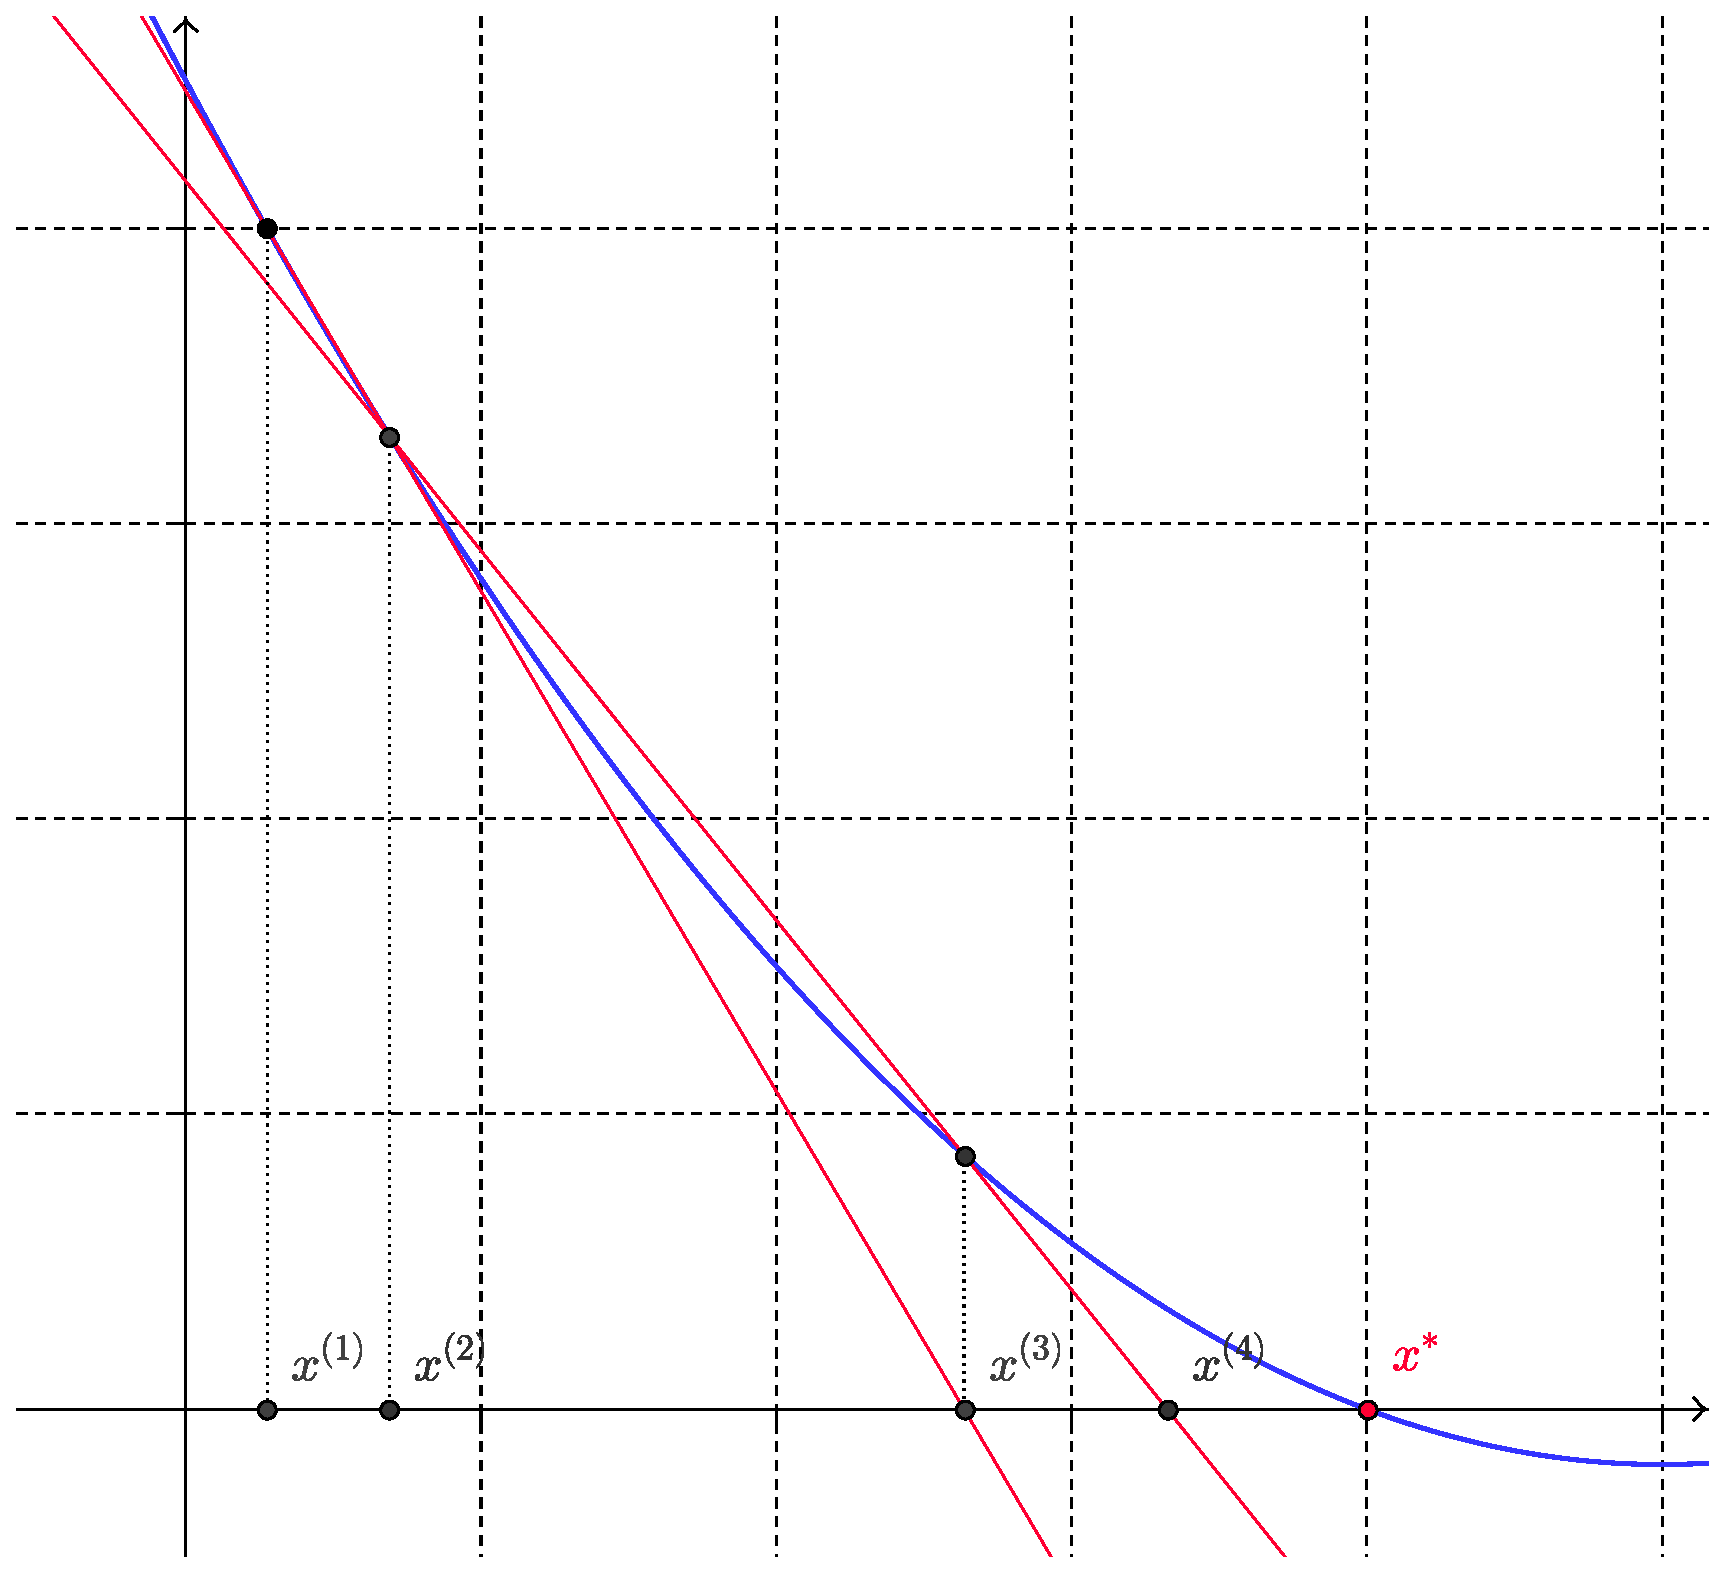
\includegraphics[width=0.8\textwidth]{./cap_eq1d/dados/fig_secante_geointerp/fig_secante_geointerp}
  \caption{Interpretação geométrica das iterações do método da secante. Veja no \href{https://github.com/phkonzen/notas/blob/master/src/MatematicaNumerica/cap_eq1d/dados/fig_secante_geointerp/fig_secante_geointerp.ggb}{Geogebra}.}
  \label{fig:secante_geointerp}
\end{figure}


\begin{obs}
  A interpretação geométrica do método da secante pode nos ajudar a escolher as aproximações iniciais $x^{(1)}$ e $x^{(2)}$. Como uma boa prática, escolhemo-las próximas do zero (por inspeção gráfica), tomando $x^{(2)}$ como uma aproximação melhor que $x^{(1)}$. 
\end{obs}

\subsection{Análise de convergência}

Pode-se mostrar\footnote{Veja, por exemplo, \href{https://www.ufrgs.br/reamat/CalculoNumerico/livro-oct/sdeduv-metodo_das_secantes.html}{Seção 3.5.2 do livro ``Cálculo Numérico''} do projeto \href{https://www.ufrgs.br/reamat}{REAMAT}.} que a taxa de convergência do método da secante é superlinear com
\begin{equation}
  |x^{(k+1)}-x^*| \leq C|x^{(k)}-x^*|^{\pmb{\varphi}},
\end{equation}
onde $\varphi = (1+\sqrt{5})/2\approx 1,618$ (razão áurea) e $x^*$ é o zero de $f$.


\begin{ex}\label{ex:secante_taxa}
  Consideremos o problema de encontrar o zero da função
  \begin{equation}
    f(x) = \sen^2\left(x+\frac{\pi}{4}\right) - x^3 + \frac{\pi}{4}x^2 + \frac{5\pi^2}{16}x + \frac{3\pi^3}{64}.
  \end{equation}
  no intervalo $[2,3]$. Este problema foi construído de forma que $x^* = 3\pi/4$ é um zero de $f$. Agora, fazendo as iterações do método da secante com aproximações iniciais $x^{(1)}=2,6$ e $x^{(2)}=2,5$, obtemos os resultados apresentados na Tabela \ref{tab:ex_secante_taxa}.

\begin{table}[h!]
  \centering
  \begin{tabular}{r|cc}
    $k$ & $x^{(k)}$ & $|x^{(k)}-x^*|$ \\\hline
    3 & $2,3728$ & $1,7\E-02$ \\
    4 & $2,3574$ & $1,2\E-03$ \\
    5 & $2,3562$ & $1,1\E-05$ \\
    6 & $2,3562$ & $7,0\E-09$ \\\hline
  \end{tabular}
  \caption{Resultados referentes ao Exemplo \ref{ex:secante_taxa}.}
  \label{tab:ex_secante_taxa}
\end{table}

\ifisoctave
Os resultados apresentados na Tabela \ref{tab:ex_secante_taxa} podem ser computados no \verb+GNU Octave+ com o seguinte \href{https://github.com/phkonzen/notas/blob/master/src/MatematicaNumerica/cap_eq1d/dados/ex_secante_taxa/ex_secante_taxa.m}{código}:
\verbatiminput{./cap_eq1d/dados/ex_secante_taxa/ex_secante_taxa.m}
\fi
\end{ex}


\begin{obs}(\normalfont{Zeros de multiplicidade par.})
  A taxa de convergência superlinear do método da secante não se mantém para o caso de $x^*$ ser um zero de multiplicidade par. Para contornar isso, pode-se aplicar o método à derivada da $f$.
\end{obs}

\begin{obs}(\normalfont{Cancelamento catastrófico.})
  Conforme convergem as iterações do método da secante, o denominador $f(x^{(k)})-f(x^{(k-1)})$ pode convergir rapidamente para zero, ocasionando uma divisão por zero.
\end{obs}


\subsection*{Exercícios}

\begin{exer}\label{exer:secante_1}
  Use o método da secante para obter uma aproximação do zero de $f(x)=x^3\sen(x)-\cos(x)$ no intervalo $[0,5, 1]$ com precisão de $10^{-5}$.
\end{exer}
\begin{resp}
    \ifisoctave 
  \href{https://github.com/phkonzen/notas/blob/master/src/MatematicaNumerica/cap_eq1d/dados/exer_secante_1/exer_secante_1.m}{Código.} 
  \fi
  $9,1581\times 10^{-1}$
\end{resp}

\begin{exer}\label{exer:secante_multpar}
  Use o método da secante para obter uma aproximação do zero de
  \begin{equation}
    f(x) = (-x^2+1,154x-0,332929)\cos(x) + x^2 - 1,154x + 0,332929
  \end{equation}
no intervalo $(0,55, ~0,65)$ com precisão de $10^-5$.
\end{exer}
\begin{resp}
    \ifisoctave 
  \href{https://github.com/phkonzen/notas/blob/master/src/MatematicaNumerica/cap_eq1d/dados/exer_secante_multpar/exer_secante_multpar.m}{Código.} 
  \fi
  $5,7700\times 10^{-1}$
\end{resp}

%Este trabalho está licenciado sob a Licença Atribuição-CompartilhaIgual 4.0 Internacional Creative Commons. Para visualizar uma cópia desta licença, visite http://creativecommons.org/licenses/by-sa/4.0/deed.pt_BR ou mande uma carta para Creative Commons, PO Box 1866, Mountain View, CA 94042, USA.

\chapter{Métodos diretos para sistemas lineares}\label{cap_sl_direto}
\thispagestyle{fancy}

Neste capítulo, discutiremos sobre métodos diretos para a resolução de sistemas lineares de $n$-equações com $n$-incógnitas. Isto é, sistemas que podem ser escritos na seguinte forma algébrica
\begin{align}
  a_{11}x_1 + a_{12}x_2 + \cdots + a_{1n}x_n &= b_1\\
  a_{21}x_1 + a_{22}x_2 + \cdots + a_{2n}x_n &= b_2\\
  &\vdots \\
  a_{n1}x_1 + a_{n2}x_2 + \cdots + a_{nn}x_n &= b_n.
\end{align}

\section{Eliminação gaussiana}\label{cap_sl_direto_sec_egauss}

Um sistema linear
\begin{align}
  a_{11}x_1 + a_{12}x_2 + \cdots + a_{1n}x_n &= b_1 \label{eq:sl_fa_1}\\
  a_{21}x_1 + a_{22}x_2 + \cdots + a_{2n}x_n &= b_2\\
  &\vdots \\
  a_{n1}x_1 + a_{n2}x_2 + \cdots + a_{nn}x_n &= b_n.\label{eq:sl_fa_n}
\end{align}
pode ser escrito na forma matricial
\begin{equation}
  A\pmb{x} = \pmb{b},
\end{equation}
onde $A = [a_{ij}]_{i,j=1}^{n,n}$ é chamada de matriz dos coeficientes, $\pmb{x}=(x_1, x_2, \dotsc, x_n)$ é o vetor (coluna) das incógnitas e $\pmb{b}=(b_1, b_2, \dotsc, b_n)$ é o vetor (coluna) dos termos constantes.

Outra forma matricial de representar o sistema \eqref{eq:sl_fa_1}-\eqref{eq:sl_fa_n} é pela chamada matriz estendida
\begin{equation}
  E = [A ~\pmb{b}].
\end{equation}
No caso, $E$ é a seguinte matriz $n \times (n+1)$
\begin{equation}
  E =
  \begin{bmatrix}
    a_{11} & a_{12} & \cdots & a_{1n} & b_1\\
    a_{21} & a_{22} & \cdots & a_{2n} & b_2\\
    \vdots & \vdots & \vdots & \vdots & \vdots\\
    a_{n1} & a_{n2} & \cdots & a_{nn} & b_n
  \end{bmatrix}
\end{equation}

O método de eliminação gaussiana consistem em realizar operações sobre as equações (sobre as linhas) do sistema \eqref{eq:sl_fa_1}-\eqref{eq:sl_fa_n} (da matriz estendida $E$) de forma a reescrevê-lo como um sistema triangular, ou diagonal. Para tanto, podemos utilizar as seguintes operações:
\begin{enumerate}[1.]
\item permutação entre as equações (linhas) ($E_i \leftrightarrow E_j$).
\item multiplicação de uma equação (linha) por um escalar não nulo ($E_i \leftarrow \lambda E_i$).
\item substituição de uma equação (linha) por ela somada com a multiplicação de uma outra por um escalar não nulo ($E_i \leftarrow E_i + \lambda E_j$).
\end{enumerate}

\begin{ex}\label{ex:egauss_exec}
  O sistema linear
  \begin{align}
    -2x_1 - 3x_2 + 2x_3 + 3x_4 &= 10\label{eq:ex_egauss_exec_sl_1}\\
    -4x_1 - 6x_2 + 6x_3 + 6x_4 &= 20\\
    -2x_1 + 4x_3 + 6x_4 &= 10\\
    4x_1 + 3x_2 - 8x_3 - 6x_4 &= -17\label{eq:ex_egauss_exec_sl_4}
  \end{align}
pode ser escrito na forma matricial $A\pmb{x}=\pmb{b}$, onde
\begin{equation}
  A =
  \begin{bmatrix}
    -2 & -3 & 2 & 3\\
    -4 & -6 & 6 & 6\\
    -2 & 0 & 4 & 6 \\
    4 & 3 & -8 & -6
  \end{bmatrix},
\end{equation}
$\pmb{x} = (x_1, x_2, x_3, x_4)$ e $\pmb{b} = (10, 20, 10, -17)$. Sua matriz estendida é
\begin{equation}
  E =
  \begin{bmatrix}
    -2 & -3 & 2 & 3 & 10\\
    -4 & -6 & 6 & 6 & 20\\
    -2 & 0 & 4 & 6 & 10\\
    4 & 3 & -8 & -6 & -17
  \end{bmatrix}
\end{equation}
Então, usando o método de eliminação gaussiana, temos
\begin{align}
  E &=
  \begin{bmatrix}
    -2 & -3 & 2 & 3 & 10\\
    -4 & -6 & 6 & 6 & 20\\
    -2 & 0 & 4 & 6 & 10\\
    4 & 3 & -8 & -6 & -17
  \end{bmatrix}
  \begin{matrix}
  \\
  E_2\leftarrow E_2 - (e_{21}/\pmb{e_{11}})E_1\\
  \\
  \\
  \end{matrix}\\
  &\sim 
  \begin{bmatrix}
    \pmb{-2} & -3 & 2 & 3 & 10\\
    0 & 0 & 2 & 0 & 0\\
    -2 & 0 & 4 & 6 & 10\\
    4 & 3 & -8 & -6 & -17
  \end{bmatrix}
  \begin{matrix}
  \\
  \\
  E_3\leftarrow E_3 - (e_{31}/\pmb{e_{11}})E_1\\
  \\
  \end{matrix}\\
  &\sim 
  \begin{bmatrix}
    \pmb{-2} & -3 & 2 & 3 & 10\\
    0 & 0 & 2 & 0 & 0\\
    0 & 3 & 2 & 3 & 0\\
    4 & 3 & -8 & -6 & -17
  \end{bmatrix}
  \begin{matrix}
  \\
  \\
  \\
  E_4\leftarrow E_4 - (e_{41}/\pmb{e_{11}})E_1\\
  \end{matrix}\\  
&\sim 
  \begin{bmatrix}
    \pmb{-2} & -3 & 2 & 3 & 10\\
    0 & 0 & 2 & 0 & 0\\
    0 & \pmb{3} & 2 & 3 & 0\\
    0 & -3 & -4 & 0 & 3
  \end{bmatrix}
  \begin{matrix}
  \\
  E_2 \leftrightarrow E_3\\
  \\
  \\
  \end{matrix}\\
&\sim 
  \begin{bmatrix}
    \pmb{-2} & -3 & 2 & 3 & 10\\
    0 & \pmb{3} & 2 & 3 & 0\\
    0 & 0 & 2 & 0 & 0\\
    0 & -3 & -4 & 0 & 3
  \end{bmatrix}
  \begin{matrix}
  \\
  \\
  \\
  E_4 \leftarrow E_4 - (e_{42}/\pmb{e_{22}})E_2\\
  \end{matrix}\\
&\sim 
  \begin{bmatrix}
    \pmb{-2} & -3 & 2 & 3 & 10\\
    0 & 3 & 2 & 3 & 0\\
    0 & 0 & \pmb{2} & 0 & 0\\
    0 & 0 & -2 & 3 & 3
  \end{bmatrix}
  \begin{matrix}
  \\
  \\
  \\
  E_4 \leftarrow E_4 - (e_{43}/\pmb{e_{33}})E_3\\
  \end{matrix}\\
    &\sim 
      \begin{bmatrix}
        \pmb{-2} & -3 & 2 & 3 & 10\\
        0 & \pmb{3} & 2 & 3 & 0\\
        0 & 0 & \pmb{2} & 0 & 0\\
        0 & 0 & 0 & \pmb{3} & 3
      \end{bmatrix}
\end{align}
Esta última matriz estendida é chamada de \emph{matriz escalonada} do sistema. Desta, temos que \eqref{eq:ex_egauss_exec_sl_1}-\eqref{eq:ex_egauss_exec_sl_4} é equivalente ao seguinte sistema triangular
\begin{align}
  -2x_1 - 3x_2 + 2x_3 + 3x_4 &= 10\\
  3x_2 + 2x_3 + 3x_4 &= 0\\
  2x_3 &= 0\\
  3x_4 &= 3.
\end{align}
Resolvendo da última equação para a primeira, temos
\begin{align}
  x_4 &= 1,\\
  x_3 &= 0,\\
  x_2 &= \frac{-2x_3 - 3x_4}{3} = -1,\\
  x_1 &= \frac{10 + 3x_2 - 3x_3 - 3x_4}{-2} = -2.
\end{align}

\ifisoctave
No \verb+GNU Octave+, podemos fazer as computações acima com o seguinte \href{https://github.com/phkonzen/notas/blob/master/src/MatematicaNumerica/cap_sl_direto/dados/ex_egauss_exec/ex_egauss_exec.m}{código}:
\verbatiminput{./cap_sl_direto/dados/ex_egauss_exec/ex_egauss_exec.m}
\fi
\end{ex}

\begin{obs}
  Para a resolução de um sistema linear $n \times n$, o método de eliminação gaussiana demanda
  \begin{equation}
    \frac{n^3}{3} + n^2 - \frac{n}{3}
  \end{equation}
multiplicações/divisões e
\begin{equation}
  \frac{n^3}{3} + \frac{n^2}{2} - \frac{5n}{6}
\end{equation}
adições/subtrações \cite{Burden2015a}.
\end{obs}

Com o mesmo custo computacional, podemos utilizar o método de eliminação gaussiana para transformar o sistema dado em um sistema diagonal.

\begin{ex}\label{ex:egauss_reduzida}
  Voltando ao exemplo anterior (Exemplo \ref{ex:egauss_exec}, vimos que a matriz estendida do sistema \eqref{eq:ex_egauss_exec_sl_1}-\eqref{eq:ex_egauss_exec_sl_4} é equivalente a
  \begin{equation}
    E \sim       
    \begin{bmatrix}
        -2 & -3 & 2 & 3 & 10\\
        0 & 3 & 2 & 3 & 0\\
        0 & 0 & 2 & 0 & 0\\
        0 & 0 & 0 & 3 & 3
      \end{bmatrix}.
  \end{equation}
Então, podemos continuar aplicando o método de eliminação gaussiana, agora de baixo para cima, até obtermos um sistema diagonal equivalente. Vejamos
\begin{align}
  E &\sim       
      \begin{bmatrix}
        -2 & -3 & 2 & 3 & 10\\
        0 & 3 & 2 & 3 & 0\\
        0 & 0 & 2 & 0 & 0\\
        0 & 0 & 0 & \pmb{3} & 3
      \end{bmatrix}
      \begin{array}{l}
      E_1 \leftarrow E_1 - (e_{14}/e_{44})E_4\\
      E_2 \leftarrow E_2 - (e_{24}/e_{44})E_4\\
      \\
      \\
    \end{array}\\
    &\sim       
      \begin{bmatrix}
        -2 & -3 & 2 & 0 & 7\\
        0 & 3 & 2 & 0 & -3\\
        0 & 0 & \pmb{2} & 0 & 0\\
        0 & 0 & 0 & 3 & 3
      \end{bmatrix}
      \begin{array}{l}
      E_1 \leftarrow E_1 - (e_{13}/e_{33})E_3\\
      E_2 \leftarrow E_2 - (e_{23}/e_{33})E_3\\
      \\
      \\
    \end{array}\\
    &\sim       
      \begin{bmatrix}
        -2 & -3 & 0 & 0 & 4\\
        0 & \pmb{3} & 0 & 0 & -3\\
        0 & 0 & 2 & 0 & 0\\
        0 & 0 & 0 & 3 & 3
      \end{bmatrix}
      \begin{array}{l}
      E_1 \leftarrow E_1 - (e_{12}/e_{22})E_2\\
      \\
      \\
      \\
    \end{array}\\
    &\sim       
      \begin{bmatrix}
        \pmb{-2} & 0 & 0 & 0 & 4\\
        0 & \pmb{3} & 0 & 0 & -3\\
        0 & 0 & \pmb{2} & 0 & 0\\
        0 & 0 & 0 & \pmb{3} & 3
      \end{bmatrix}
      \begin{array}{l}
      E_1 \leftarrow E_1/e_{11}\\
      E_2 \leftarrow E_2/e_{22}\\
      E_3 \leftarrow E_3/e_{33}\\
      E_4 \leftarrow E_4/e_{44}\\
    \end{array}\\
    &\sim       
      \begin{bmatrix}
        1 & 0 & 0 & 0 & -2\\
        0 & 1 & 0 & 0 & -1\\
        0 & 0 & 1 & 0 & 0\\
        0 & 0 & 0 & 1 & 1
      \end{bmatrix}
  \end{align}
Esta última matriz é chamada de matriz escalonada reduzida (por linhas) e a solução do sistema encontra-se em sua última coluna, i.e. $\pmb{x} = (-2, -1, 0, 1)$.

\ifisoctave
No \verb+GNU Octave+, podemos fazer as computações acima com o seguinte \href{https://github.com/phkonzen/notas/blob/master/src/MatematicaNumerica/cap_sl_direto/dados/ex_egauss_reduzida/ex_egauss_reduzida.m}{código}:
\verbatiminput{./cap_sl_direto/dados/ex_egauss_reduzida/ex_egauss_reduzida.m}
\fi
\end{ex}

\subsection*{Exercícios}

\begin{exer}\label{exer:egauss_reduzida}
  Use o método de eliminação gaussiana para obter a matriz escalonada reduzida do seguinte sistema
  \begin{align}
    -3x_1 + 2x_2 -5x_4 + x_5 &= -23\\
    -x_2 -3x_4 &= 9\\
    -2x_1 -x_2 + x_3 &= -1\\
    2x_2 - 4x_3 + 3x_4 &= 8\\
    x_1 - 3x_3 - x_4 &= 11
  \end{align}
\end{exer}
\begin{resp}
    \ifisoctave 
  \href{https://github.com/phkonzen/notas/blob/master/src/MatematicaNumerica/cap_sl_direto/dados/exer_egauss_reduzida/exer_egauss_reduzida.m}{Código.} 
  \fi
  $$
  \begin{bmatrix}
    1 & 0 & 0 & 0 & 0 & 1\\
    0 & 1 & 0 & 0 & 0 & -3\\
    0 & 0 & 1 & 0 & 0 & -2\\
    0 & 0 & 0 & 1 & 0 & 2\\
    0 & 0 & 0 & 0 & 1 & -4\\
  \end{bmatrix}
  $$
\end{resp}

\begin{exer}\label{exer:egauss_arredondamento}
  Use o método de eliminação gaussiana para obter a matriz escalonada reduzida do seguinte sistema
  \begin{align}
    -10^{-12}x_1 + 20x_2 - 3x_3 &= -1\\
    2,001x_1 + 10^{-5}x_2 - x_3 &= -2\\
    4x_1 - 2x_2 + x_3 &= 0,1
  \end{align}
\end{exer}
\begin{resp}
  \ifisoctave 
  \href{https://github.com/phkonzen/notas/blob/master/src/MatematicaNumerica/cap_sl_direto/dados/exer_egauss_arredondamento/exer_egauss_arredondamento.m}{Código.} 
  \fi
  $$
  \begin{bmatrix}
   1.0000 &  0.0000 &  0.0000 & -3.9435\E-1\\
  -0.0000 &  1.0000 & -0.0000 & -2.3179\E-1\\
   0.0000 &  0.0000 &  1.0000 &  1.2120\E+0
  \end{bmatrix}
  $$
\end{resp}

\section{Norma e número de condicionamento}

Nesta seção, fazemos uma rápida discussão sobre normas de vetores e matrizes, bem como do número de condicionamento de uma matriz.

\subsection{Norma $L^2$}

A norma $L^2$ de um dado vetor $v = (v_1, v_2, \dotsc, v_n) \in \mathbb{R^n}$ é definida por
\begin{equation}
  \|v\| := \sqrt{v_1^2 + v_2^2 + \cdots + v_n^2}.
\end{equation}

\begin{prop}
  Dados os vetores $u,v \in \mathbb{R^n}$ e um escalar $\lambda\in\mathbb{R}$, temos:
  \begin{enumerate}[a)]
  \item $\|v\| \geq 0$.
  \item $\|v\| = 0 \Leftrightarrow v=0$.
  \item $\|\lambda v\| = |\lambda|\cdot \|v\|$.
  \item $\|u+v\| \leq \|u\| + \|v\|$ (desigualdade triangular).
  \item $u\cdot v \leq \|u\|\cdot\|v\|$ (desigualdade de Cauchy-Schwarz).
  \end{enumerate}
\end{prop}

\begin{ex}\label{ex:norma_vetor}
  A norma $L^2$ do vetor $v = (1, -2, 3, -4)$ é
  \begin{align}
    \|v\| &= \sqrt{v_1^2 + v_2^2 + v_3^2 + v_4^2}\\
    &= \sqrt{1^2 + (-2)^2 + 3^2 + (-4)^2}\\
    &= 5,4772.
  \end{align}

\ifisoctave
No \verb+GNU Octave+, podemos fazer as computações acima com o seguinte \href{https://github.com/phkonzen/notas/blob/master/src/MatematicaNumerica/cap_sl_direto/dados/ex_norma_vetor/ex_norma_vetor.m}{código}:
\verbatiminput{./cap_sl_direto/dados/ex_norma_vetor/ex_norma_vetor.m}
\fi
\end{ex}


A norma $L^2$ induzida de uma dada matriz real $A = [a_{ij}]_{i,j=1}^n$ é definida por
\begin{equation}
  \|A\| := \sup_{x\in\mathbb{R}^n, \|x\|=1} \|Ax\|.
\end{equation}
Pode-se mostrar que
\begin{equation}
  \|A\| = \sqrt{\lambda_{max}(A^TA)},
\end{equation}
onde $\lambda_{max}(A^TA) := \max\{|\lambda|;~\lambda\text{ é autovalor de }A^TA\}$.

\begin{prop}
  Dadas as matrizes reais $A, B$ $n\times n$, um vetor $v\in\mathbb{R}^2$ e um escalar $\lambda$, temos
  \begin{enumerate}[a)]
  \item $\|A\| \geq 0$.
  \item $\|A\|=0 \Leftrightarrow A=0$.
  \item $\|\lambda A\| = |\lambda|\cdot \|A\|$.
  \item $\|A+B\| \leq \|A\| + \|B\|$ (desigualdade triangular).
  \item $\|AB\| \leq \|A\|\|B\|$.
  \item $\|Av\| \leq \|A\|\|v\|$.
  \end{enumerate}
\end{prop}

\begin{ex}\label{ex:norma_matriz}
  A matriz
  \begin{equation}
    A =
    \begin{bmatrix}
      1 & -1 & 2\\
      -2 & \pi & 4\\
      7 & -5 & \sqrt{2}
    \end{bmatrix}
  \end{equation}
tem norma $L^2$
\begin{equation}
  \|A\| = 9,3909.
\end{equation}

\ifisoctave
No \verb+GNU Octave+, podemos fazer as computações acima com o seguinte \href{https://github.com/phkonzen/notas/blob/master/src/MatematicaNumerica/cap_sl_direto/dados/ex_norma_matriz/ex_norma_matriz.m}{código}:
\verbatiminput{./cap_sl_direto/dados/ex_norma_matriz/ex_norma_matriz.m}
\fi
\end{ex}

\subsection{Número de condicionamento}

O número de condicionamento de uma matriz é uma medida referente a propagação de erros de ocorre da sua aplicação. Mais especificamente, assumamos que seja dada uma matriz invertível $A = [a_{ij}]_{i,j=1}^{n,n}$, um vetor $x\in\mathbb{R}^n$ e uma perturbação $\delta_x\in\mathbb{R}^n$. Além disso, sejam
\begin{align}
  y &= Ax\\
  y + \delta_y &= A(x+\delta_x).
\end{align}
Ou seja, $\delta_y$ é a perturbação em $y$ propagada da aplicação de $A$ em $x$ com perturbação $\delta_x$.

Agora, podemos estimar a razão entre os erros relativos $e_{rel}(y) := \|\delta_y\|/\|y\|$ e $e_{rel}(x) := \|\delta_x\|/\|x\|$ da seguinte forma 
\begin{align}
  \frac{\frac{\|y\|}{\|\delta_y\|}}{\frac{\|x\|}{\|\delta_x\|}} &= \frac{\|y\|}{\|\delta_y\|}\frac{\|\delta_x\|}{\|x\|}\\
  &=\frac{\|Ax\|}{\|\delta_y\|}\frac{\|A^{-1}\delta_y\|}{\|x\|} \\
  &\leq \frac{\|A\|\|x\|\|A^{-1}\|\|\delta_y\|}{\|\delta_y\|\|x\|}\\
  &\leq \|A\|\|A^{-1}\|.
\end{align}
Logo, temos a seguinte estimativa de propagação de erro
\begin{equation}
  e_{rel}(y) \leq \|A\|\|A^{-1}\|e_{rel}(x).
\end{equation}

Isto nos motiva a definir o \emph{número de condicionamento} da matriz $A$ por
\begin{equation}
  \kappa(A) := \|A\|\|A^{-1}\|.
\end{equation}

\begin{obs}
  A matriz identidade tem o menor número de condicionamento, o qual é
  \begin{equation}
    \kappa(I) = 1.
  \end{equation}
\end{obs}

\begin{ex}\label{ex:kappa}
  Um exemplo de uma matriz bem condicionada é
  \begin{equation}
    A =
    \begin{bmatrix}
      1 & -1 & 2\\
      -2 & \pi & 4\\
      7 & -5 & \sqrt{2}
    \end{bmatrix},
  \end{equation}
  cujo número de condicionamento é $\kappa(A) = 13,997$.

  Já, a matriz
  \begin{equation}
    B =
    \begin{bmatrix}
      1 & 0 & 0\\
      0 & 0 & -2\\
      10^{5} & 10^{-4} & 10^{5}
    \end{bmatrix},    
  \end{equation}
  tem número de condicionamento
  \begin{equation}
    \kappa(B) = 1,5811\times 10^{14},
  \end{equation}
  o que indica que $B$ é uma matriz mal condicionada.
\end{ex}

\subsection*{Exercícios}

\begin{exer}\label{exer:norma_numcond}
  Considere o seguinte sistema linear
  \begin{align}
    10^{-12}x_1 + 20x_2 + 3x_3 &= -1,\\
    2,001x_1 + 10^{-5}x_2 + - x_3 &= -2,\\
    x_1 - 2x_2 - 0,1x_3 &= 0,1.
  \end{align}
  \begin{enumerate}[a)]
  \item Compute a norma $L^2$ do vetor dos termos constantes deste sistema.
  \item Compute a norma $L^2$ da matriz dos coeficientes deste sistema.
  \item Compute o número de condicionamento da matriz dos coeficientes deste sistema.
  \end{enumerate}
\end{exer}
\begin{resp}
  \ifisoctave 
  \href{https://github.com/phkonzen/notas/blob/master/src/MatematicaNumerica/cap_sl_direto/dados/exer_norma_numcond/exer_norma_numcond.m}{Código.} 
  \fi
  a) $2,2383$; b) $2,0323\E+1$; c) $3,5128\E+1$
\end{resp}


\section{Método de eliminação gaussiana com pivotamento parcial com escala}

O método de eliminação gaussiana é suscetível a propagação dos erros de arredondamento, em particular, quando os pivôs são números próximos de zero. Isto pode ser mitigado com o chamado pivotamento parcial com escala. Nesta variação do método de eliminação gaussiana, o pivô é escolhido como sendo o candidato que é o maior em relação aos elementos em sua linha.

Dado um sistema $Ax = b$ com $n$-equações e $n$-incógnitas, o método pode ser descrito pelo seguinte pseudo-código:
\begin{enumerate}
 \item $E \leftarrow [A ~ b]$.
 \item Para $i=1, 2, \dotsc, n$, faça $s_i \leftarrow \max_{1\leq j \leq n}|e_{i,j}|$.
 \item Para $i=1, 2, \dotsc, n-1$:
   \begin{enumerate}[3.1]
   \item Compute $j$ tal que
     \begin{equation}
       \frac{e_{j,i}}{s_j} \geq \frac{e_{k,i}}{s_k},\quad\forall k=i, i+1, \dotsc, n.
     \end{equation}
     \item Permute as linhas $i$ e $j$, i.e. $E_i \leftrightarrow E_j$.
     \item Para $j=i+1, i+2, \dotsc, n$:
       \begin{enumerate}[3.3.1]
       \item $E_j \leftarrow E_j - \frac{e_{ji}}{e_{ii}}E_i$.
       \end{enumerate}
   \end{enumerate}
 \item Para $i=n, n-1, \dotsc, 2$:   
   \begin{enumerate}[4.1]
     \item Para $j=i-1, i-2, \dotsc, 1$:
       \begin{enumerate}[4.1.1]
         \item $E_j \leftarrow E_j - \frac{e_{ji}}{e_{ii}}E_i$.
       \end{enumerate}
   \end{enumerate}
\end{enumerate}

\begin{ex}\label{ex:egauss_pivo}
  Vamos empregar o método de eliminação gaussiana com pivotamento parcial com escala para resolvermos o seguinte sistema linear
  \begin{align}
    10^{-12}x_1 + 20x_2 + 3x_3 &= -1,\\
    2,001x_1 + 10^{-5}x_2 + - x_3 &= -2,\\
    x_1 - 2x_2 - 0,1x_3 &= 0,1.
  \end{align}
  Para tanto, tomamos a matriz estendida
  \begin{equation}
    E =
    \begin{bmatrix}
      10^{-12} & 20 & 3 & -1\\
      2,001 & 10^{-5} & -1 & -2\\
      1 & -2 & -0,1 & 0,1
    \end{bmatrix}
  \end{equation}
  e computamos os valores máximos em módulo dos elementos de cada linha da matriz $A$, i.e.
  \begin{equation}
    s = (20, 2,001, 2).
  \end{equation}
  Agora, observamos que $e_{2,1}$ é o maior pivô em escala, pois
  \begin{equation}
    \frac{e_{11}}{s_1} = 5\times 10^{-14}, \frac{e_{21}}{s_2} = 1, \frac{e_{31}}{s_3}=0,5.
  \end{equation}
  Então, fazemos a permutação entre as linhas $1$ e $2$, de forma a obtermos
  \begin{equation}
    E =
    \begin{bmatrix}
      2,001 & 10^{-5} & -1 & -2\\
      10^{-12} & 20 & 3 & -1\\
      1 & -2 & -0,1 & 0,1
    \end{bmatrix}    
  \end{equation}
  Em seguida, eliminamos abaixo do pivô, e temos
  \begin{equation}
    E =
    \begin{bmatrix}
      2,001 & 10^{-5} & -1 & -2\\
      0 & 20 & 3 & -1\\
      0 & -2 & 3,9975\times 10^{-1} & 1,0995
    \end{bmatrix}
  \end{equation}
  Daí, o novo pivô é escolhido como $e_{22}$, pois ambos candidatos tem o mesmo valor em escala
  \begin{equation}
    \frac{e_{2,2}}{s_2} = 1, \frac{e_{3,2}}{s_3} = 1.
  \end{equation}
  Logo, eliminamos abaixo do pivô para obtermos
  \begin{equation}
    E =
    \begin{bmatrix}
      2,001 & 10^{-5} & -1 & -2\\
      0 & 20 & 3 & -1\\
      0 & 0 & 6,9975\times 10^{-1} & 9,9950
    \end{bmatrix}
  \end{equation}
  Procedendo a eliminação para cima, obtemos a matriz escalonada reduzida
  \begin{equation}
    E =
    \begin{bmatrix}
      1 & 0 & 0 & -2.8567\E-1\\
      0 & 1 & 0 & -2.6425\E-1\\
      0 & 0 & 1 & 1,4284\E+0
    \end{bmatrix}
  \end{equation}

\ifisoctave
No \verb+GNU Octave+, podemos fazer as computações acima com o seguinte \href{https://github.com/phkonzen/notas/blob/master/src/MatematicaNumerica/cap_sl_direto/dados/ex_egauss_pivo/ex_egauss_pivo.m}{código}:
\verbatiminput{./cap_sl_direto/dados/ex_egauss_pivo/ex_egauss_pivo.m}
\fi
\end{ex}

\subsection*{Exercícios}

\begin{exer}\label{exer:egauss_pivo_exec}
  Use o método de eliminação gaussiana com pivotamento parcial com escala para obter a matriz escalonada reduzida do seguinte sistema
  \begin{align}
    -2\times 10^{-12}x_1 + 10x_2 - 3\times 10^{-4}x_3 &= 2\\
    10^5x_1 + 10^{-13}x_2 - x_3 &= -2\\
    x_1 - 2x_2 + 3\times 10^{-7}x_3 &= 4
  \end{align}
\end{exer}
\begin{resp}
  \ifisoctave 
  \href{https://github.com/phkonzen/notas/blob/master/src/MatematicaNumerica/cap_sl_direto/dados/exer_egauss_pivo_exec/exer_egauss_pivo_exec.m}{Código.} 
  \fi
  $$
  \begin{bmatrix}
   1,0000 &  0,0000 &  0,0000 & 6,2588\E-1\\
   0,0000 &  1,0000 &  0,0000 & -1,6777\E+0\\
   0,0000 &  0,0000 &  1,0000 & 6,2589\E+4
  \end{bmatrix}
  $$
\end{resp}

%Este trabalho está licenciado sob a Licença Atribuição-CompartilhaIgual 4.0 Internacional Creative Commons. Para visualizar uma cópia desta licença, visite http://creativecommons.org/licenses/by-sa/4.0/deed.pt_BR ou mande uma carta para Creative Commons, PO Box 1866, Mountain View, CA 94042, USA.

\chapter{Métodos iterativos para sistemas lineares}\label{cap_sl_iter}
\thispagestyle{fancy}

\section{Métodos de Jacobi e de Gauss-Seidel}\label{cap_sl_iter_sec_jgs}

Nesta seção, discutiremos os métodos de Jacobi\footnote{Carl Gustav Jacob Jacobi, 1804 - 1851, matemático alemão. Fonte: \href{https://en.wikipedia.org/wiki/Carl_Gustav_Jacob_Jacobi}{Wikipedia}.} e de Gauss-Seidel\footnote{Johann Carl Friedrich Gauss, 1777 - 1855, matemático alemão. Philipp Ludwig von Seidel, 1821 - 1896, matemático alemão. Fonte: \href{https://en.wikipedia.org/wiki/Philipp_Ludwig_von_Seidel}{Wikipedia}.} para a aproximação da solução de sistemas lineares.

\subsection{Método de Jacobi}

Dado um sistema $A\pmb{x} = \pmb{b}$ com $n$ equações e $n$ incógnitas, consideramos a seguinte decomposição da matriz $A = L + D + U$:
\begin{align}
  A &=
  \begin{bmatrix}
    a_{11} & a_{12} & a_{13} & \ldots & a_{1n}\\
    a_{21} & a_{22} & a_{23} & \ldots & a_{2n}\\
    a_{31} & a_{32} & a_{33} & \ldots & a_{3n}\\
    \vdots & \vdots & \vdots & \ldots & \vdots\\
    a_{n1} & a_{n2} & a_{n3} & \ldots & a_{nn}\\
  \end{bmatrix}\\
    &= \underbrace{\begin{bmatrix}
    0 & 0 & 0 & \ldots & 0\\
    a_{21} & 0 & 0 & \ldots & 0\\
    a_{31} & a_{32} & 0 & \ldots & 0\\
    \vdots & \vdots & \vdots & \ldots & \vdots\\
    a_{n1} & a_{n2} & a_{n3} & \ldots & 0\\
  \end{bmatrix}}_{L}\\
    &+ \underbrace{\begin{bmatrix}
    a_{11} & 0 & 0 & \ldots & 0\\
    0 & a_{22} & 0 & \ldots & 0\\
    0 & 0 & a_{33} & \ldots & 0\\
    \vdots & \vdots & \vdots & \ldots & \vdots\\
    0 & 0 & 0 & \ldots & a_{nn}\\
  \end{bmatrix}}_{D}\\
  &+ \underbrace{\begin{bmatrix}
    0 & a_{12} & a_{13} & \ldots & a_{1n}\\
    0 & 0 & a_{23} & \ldots & a_{2n}\\
    0 & 0 & a_{33} & \ldots & a_{3n}\\
    \vdots & \vdots & \vdots & \ldots & \vdots\\
    0 & 0 & 0 & \ldots & a_{nn}\\
  \end{bmatrix}}_{U}.
\end{align}
Isto é, a matriz $A$ decomposta como a soma de sua parte triangular inferior $L$, de sua diagonal $D$ e de sua parte triangular superior $U$.

Desta forma, podemos reescrever o sistema $A\pmb{x}=b$ da seguinte forma:
\begin{align}
  A\pmb{x} = \pmb{b} &\Leftrightarrow (L + D + U)\pmb{x} = \pmb{b}\\
         &\Leftrightarrow D\pmb{x} = -(L+U)\pmb{x} + \pmb{b}\\
         &\Leftrightarrow \pmb{x} = -D^{-1}(L+U)\pmb{x} + D^{-1}\pmb{b}.
\end{align}
Ou seja, resolver o sistema $A\pmb{x} = \pmb{b}$ é equivalente a resolver o problema de ponto fixo
\begin{equation}
  \pmb{x} = T_J\pmb{x} + \pmb{c}_J,
\end{equation}
onde $T_J = -D^{-1}(L+U)$ é chamada de \emph{matriz de Jacobi}\index{matriz de!Jacobi} e $\pmb{c}_J = D^{-1}\pmb{b}$ é chamado de \emph{vetor de Jacobi}\index{vetor de!Jacobi}.

\begin{ex}\label{ex:jacobi_intro}
  Consideremos o sistema linear $A\pmb{x} = \pmb{b}$ com
  \begin{equation}
    A =
    \begin{bmatrix}
      -4 & 2 & -1 \\
      -2 & 5 & 2 \\
       1 & -1 & -3
    \end{bmatrix},\quad
    \pmb{b} =
    \begin{bmatrix}
      -11\\ -7\\ 0
    \end{bmatrix}.
  \end{equation}
  Este sistema tem solução $\pmb{x} = (2, -1, 1)$. Neste caso, temos a decomposição $A = L + D + U$ com
  \begin{equation}
    L = \begin{bmatrix} 
      0 & 0 & 0 \\
      -2 & 0 & 0 \\
       1 & -1 & 0
     \end{bmatrix},\quad
    D = \begin{bmatrix}
      -4 & 0 & 0 \\
      0 & 5 & 0 \\
       0 & 0 & -3                  
     \end{bmatrix}
  \end{equation}
  e
  \begin{equation}
    U = \begin{bmatrix}
      0 & 2 & -1 \\
      0 & 0 & 2 \\
       0 & 0 & 0
    \end{bmatrix}.
  \end{equation}
  Ainda, observamos que
  \begin{align}
    T_J\pmb{x} + \pmb{c}_J &= -D^{-1}(L+U)\pmb{x} + D^{-1}\pmb{b}\\
    &= \underbrace{\begin{bmatrix}
        0 & 1/2 & 1/4 \\
        2/5 & 0 & -2/5 \\
        1/3 & -1/3 & 0
      \end{bmatrix}}_{T_J}
      \underbrace{\begin{bmatrix}
        2 \\
        -1 \\
        1             
      \end{bmatrix}}_{\pmb{x}} +
      \underbrace{\begin{bmatrix}
       11/4 \\
       -7/5 \\
       0
      \end{bmatrix}}_{\pmb{c}_J}\\
  &= \underbrace{\begin{bmatrix}
        2 \\
        -1 \\
        1             
      \end{bmatrix}}_{\pmb{x}}.
  \end{align}
\ifisoctave
No \verb+GNU Octave+, podemos fazer as computações acima com o seguinte \href{https://github.com/phkonzen/notas/blob/master/src/MatematicaNumerica/cap_sl_iter/dados/ex_jacobi_intro/ex_jacobi_intro.m}{código}:
\verbatiminput{./cap_sl_iter/dados/ex_jacobi_intro/ex_jacobi_intro.m}
\fi
\end{ex}

Com o exposto acima, o \emph{método de Jacobi} consiste na seguinte iteração de ponto fixo
\begin{align}
  \pmb{x}^{(1)} &= \text{aprox. inicial},\\
  \pmb{x}^{(k+1)} &= T_J\pmb{x}^{(k)} + \pmb{c}_J,\label{eq:iter_jacobi_mat}
\end{align}
onde $\pmb{x}^{(k)} = (x_1^{(k)}, x_2^{(k)}, \dotsc, x_n^{(k)})$ é a $k$-ésima aproximação (ou iterada) de Jacobi.

A iteração \eqref{eq:iter_jacobi_mat} pode ser equivalentemente escrita na seguinte forma algébrica
\begin{equation}
  x_i^{(k+1)} = \frac{{\displaystyle b_i - \sum_{\overset{j=1}{j\neq i}}^n a_{ij}x^{(k)}}}{a_{ii}},~i=1, 2, \dotsc, n,
\end{equation}
a qual não requer a computação da matriz $T_J$ e $\pmb{c}_J$.

\begin{ex}\label{ex:jacobi_exec}
  Consideremos o sistema $A\pmb{x} = \pmb{b}$ com
  \begin{equation}
    A =
    \begin{bmatrix}
      -4 & 2 & -1 \\
      -2 & 5 & 2 \\
       1 & -1 & -3
    \end{bmatrix},\quad
    \pmb{b} =
    \begin{bmatrix}
      -11\\ -7\\ 0
    \end{bmatrix}.
  \end{equation}
  Aplicando o método de Jacobi com aproximação inicial $\pmb{x}^{(1)} = (0, 0, 0)$ obtemos os resultados da Tabela \ref{tab:ex_jacobi_exec}.

  \begin{table}[h!]
    \centering
    \begin{tabular}{l|cc}
      k & $\pmb{x}^{(k)}$ & $\|A\pmb{x}^{(k)}-\pmb{b}\|$\\\hline
      1 & $(0,0,~0,0,~0,0)$ & $1,3\E+1$\\
      2 & $(2,8,~-1,4,~0,0)$ & $7,4\E+0$ \\
      3 & $(2,0,~-0,3,~1,4)$ & $4,6\E+0$ \\
      4 & $(2,3,~-1,1,~0,8)$ & $2,2\E+0$ \\
      5 & $(2,0,~-0,8,~1,1)$ & $1,4\E+0$ \\
      6 & $(2,1,~-1,1,~0,9)$ & $6,9\E-1$ \\
      7 & $(2,0,~-0,9,~1,0)$ & $4,2\E-1$ \\
      8 & $(2,0,~-1,0,~1,0)$ & $2,2\E-1$ \\
      9 & $(2,0,~-1,0,~1,0)$ & $1,3\E-1$ \\
      10 & $(2,0,~-1,0,~1,0)$ & $6,9\E-2$ \\\hline
    \end{tabular}
    \caption{Resultados referentes ao Exemplo \ref{ex:jacobi_exec}.}
    \label{tab:ex_jacobi_exec}
  \end{table}

\ifisoctave
No \verb+GNU Octave+, podemos obter os resultados reportados na Tabela \ref{tab:ex_jacobi_exec} com o seguinte \href{https://github.com/phkonzen/notas/blob/master/src/MatematicaNumerica/cap_sl_iter/dados/ex_jacobi_exec/ex_jacobi_exec.m}{código}:
\verbatiminput{./cap_sl_iter/dados/ex_jacobi_exec/ex_jacobi_exec.m}
\fi
\end{ex}

\subsection{Método de Gauss-Seidel}

Como acima, começamos considerando um sistema linear $A\pmb{x} = \pmb{b}$ e a decomposição $A = L + D + U$, onde $L$ é a parte triangular inferior de $A$, $D$ é sua parte diagonal e $U$ sua parte triangular superior. Então, observamos que
\begin{align}
  A\pmb{x} = \pmb{b} &\Leftrightarrow (L + D + U)\pmb{x} = \pmb{b}\\
  &\Leftrightarrow (L+D)\pmb{x} = -U\pmb{x} + \pmb{b}\\
  &\Leftrightarrow \pmb{x} = -(L+D)^{-1}U\pmb{x} + (L+D)^{-1}\pmb{b}.
\end{align}
Isto nos leva a iteração de Gauss-Seidel
\begin{align}
  \pmb{x}^{(1)} = \text{aprox. inicial},\\
  \pmb{x}^{(k+1)} = T_G\pmb{x}^{(k)} + \pmb{c}_G,\label{eq:iter_gs_mat}
\end{align}
onde $T_G = -(L+D)^{-1}U$ é a chamada \emph{matriz de Gauss-Seidel}\index{matriz de!Gauss-Seidel} e $\pmb{c}_G = (L+D)^{-1}\pmb{b}$ é o chamado \emph{vetor de Gauss-Seidel}\index{vetor de!Gauss-Seidel}.

Observamos, também, que a iteração \eqref{eq:iter_gs_mat} pode ser reescrita na seguinte forma algébrica
\begin{equation}
  x_i^{(k+1)} = \frac{{\displaystyle b_i - \sum_{j=1}^{i-1} a_{ij}x^{(k+1)} - \sum_{j=i+1}^{n} a_{ij}x^{(k)}}}{a_{ii}},~i=1, 2, \dotsc, n.
\end{equation}

\begin{ex}\label{ex:gs_exec}
  Consideremos o sistema $A\pmb{x} = \pmb{b}$ com
  \begin{equation}
    A =
    \begin{bmatrix}
      -4 & 2 & -1 \\
      -2 & 5 & 2 \\
       1 & -1 & -3
    \end{bmatrix},\quad
    \pmb{b} =
    \begin{bmatrix}
      -11\\ -7\\ 0
    \end{bmatrix}.
  \end{equation}
  Aplicando o método de Gauss-Seidel com aproximação inicial $\pmb{x}^{(1)} = (0, 0, 0)$ obtemos os resultados da Tabela \ref{tab:ex_gs_exec}.

  \begin{table}[h!]
    \centering
    \begin{tabular}{l|cc}
      k & $\pmb{x}^{(k)}$ & $\|A\pmb{x}^{(k)}-\pmb{b}\|$\\\hline
      1 & $(0,0,~0,0,~0,0)$ & $1,3\E+1$ \\
      2 & $(2,8,~-0,3,~1,0)$ & $2,6\E+0$ \\
      3 & $(2,3,~-0,9,~1,1)$ & $1,2\E+0$ \\
      4 & $(2,0,~-1,0,~1,0)$ & $2,5\E-1$ \\
      5 & $(2,0,~-1,0,~1,0)$ & $4,0\E-2$ \\\hline
    \end{tabular}
    \caption{Resultados referentes ao Exemplo \ref{ex:gs_exec}.}
    \label{tab:ex_gs_exec}
  \end{table}

\ifisoctave
No \verb+GNU Octave+, podemos obter os resultados reportados na Tabela \ref{tab:ex_gs_exec} com o seguinte \href{https://github.com/phkonzen/notas/blob/master/src/MatematicaNumerica/cap_sl_iter/dados/ex_gs_exec/ex_gs_exec.m}{código}:
\verbatiminput{./cap_sl_iter/dados/ex_gs_exec/ex_gs_exec.m}
\fi
\end{ex}

\subsection{Análise de convergência}

Observamos que ambos os métodos de Jacobi e de Gauss-Seidel consistem de iterações da forma
\begin{equation}
  \pmb{x}^{(k+1)} = T\pmb{x}^{(k)} + \pmb{c},~k=1, 2, \ldots,\label{eq:jgs_iter}
\end{equation}
com $x^{(1)}$ uma aproximação inicial dada, $T$ e $c$ a matriz e o vetor de iteração, respectivamente. O seguinte teorema nos fornece uma condição suficiente e necessária para a convergência de tais métodos.

\begin{teo}
  Para qualquer $\pmb{x}^{(1)}\in\mathbb{R}^n$, temos que a sequência $\{\pmb{x}^{(k+1)}\}_{k=1}^{\infty}$ dada por
  \begin{equation}
    \pmb{x}^{(k+1)} = T\pmb{x}^{(k)} + \pmb{c},
  \end{equation}
  converge para a solução única de $\pmb{x} = T\pmb{x} + \pmb{c}$ se, e somente se, $\rho(T) < 1$\footnote{$\rho(T)$ é o raio espectral da matriz $T$, i.e. o máximo dos módulos dos autovalores de $T$.}.
\end{teo}
\begin{dem}
  Veja \cite[Cap. 7, Sec. 7.3]{Burden2015a}.
\end{dem}

\begin{obs}(\normalfont{Taxa de convergência})
  Para uma iteração da forma \eqref{eq:jgs_iter}, vale
  \begin{equation}
    \|\pmb{x}^{(k)}-\pmb{x}\| \approx \rho(T)^{k-1}\|\pmb{x}^{(1)}-\pmb{x}\|,
  \end{equation}
onde $\pmb{x}$ é a solução de $\pmb{x} = T\pmb{x} + \pmb{c}$.
\end{obs}

\begin{ex}\label{ex:jacobi_exec}
  Consideremos o sistema $A\pmb{x} = \pmb{b}$ com
  \begin{equation}
    A =
    \begin{bmatrix}
      -4 & 2 & -1 \\
      -2 & 5 & 2 \\
       1 & -1 & -3
    \end{bmatrix},\quad
    \pmb{b} =
    \begin{bmatrix}
      -11\\ -7\\ 0
    \end{bmatrix}.
  \end{equation}
  Nos Exemplos \ref{ex:jacobi_exec} e \ref{ex:gs_exec} vimos que ambos os métodos de Jacobi e de Gauss-Seidel eram convergentes, sendo que este convergiu aproximadamente duas vezes mais rápido que esse. Isto é confirmado pelos raios espectrais das respectivas matrizes de iteração
  \begin{equation}
    \rho(T_J) \approx 0,56,\quad\rho(T_G) \approx 0,26.
  \end{equation}

\ifisoctave
No \verb+GNU Octave+, podemos obter os raios espectrais das matrizes de iteração de Jacobi e Gauss-Seidel com o seguinte \href{https://github.com/phkonzen/notas/blob/master/src/MatematicaNumerica/cap_sl_iter/dados/ex_jgs_conv/ex_jgs_conv.m}{código}:
\verbatiminput{./cap_sl_iter/dados/ex_jgs_conv/ex_jgs_conv.m}
\fi
\end{ex}

\begin{obs}{\normalfont{Matriz estritamente diagonal dominante}}
  Pode-se mostrar que se $A$ é uma matriz estritamente diagonal dominante, i.e. se
  \begin{equation}
    |a_{ii}| > \sum_{\overset{j=1}{j\neq i}}^n |a_{ij}|,~\forall i=1, 2, \ldots, n,
  \end{equation}
então ambos os métodos de Jacobi e de Gauss-Seidel são convergentes.
\end{obs}

\subsection*{Exercícios}

\begin{exer}\label{exer:jacobi_exec}
  Considere o seguinte sistema linear
  \begin{align}
    -4x_1 + x_2 + x_3 - x_4 &= -1\\
    5x_2 -x_3 + 2x_4 &= 3\\
    -x_1 + 4x_3 - 2x_4 &= -2\\
    x_1 -x_2 -5x_4 &= 1
  \end{align}
  Compute a quinta iterada $x^{(5)}$ do método de Jacobi aplicado a este sistema com aproximação inicial $x^{(1)} = (1, 1, -1, -1)$. Também, compute $\|Ax^{(5)} - b\|$.
\end{exer}
\begin{resp}
    \ifisoctave 
    \href{https://github.com/phkonzen/notas/blob/master/src/MatematicaNumerica/cap_sl_iter/dados/exer_jacobi_exec/exer_jacobi_exec.m}{Código.} 
  \fi
  $x^{(5)} = (-1,00256,~2,95365,~-1,95347,~0,97913)$; $\|Ax^{(5)}-b\| = 0,42244$
\end{resp}

\begin{exer}\label{exer:gs_exec}
  Considere o seguinte sistema linear
  \begin{align}
    -4x_1 + x_2 + x_3 - x_4 &= -1\\
    5x_2 -x_3 + 2x_4 &= 3\\
    -x_1 + 4x_3 - 2x_4 &= -2\\
    x_1 -x_2 -5x_4 &= 1
  \end{align}
  Compute a quinta iterada $x^{(5)}$ do método de Gauss-Seidel aplicado a este sistema com aproximação inicial $x^{(1)} = (1, 1, -1, -1)$. Também, compute $\|Ax^{(5)} - b\|$.
\end{exer}
\begin{resp}
    \ifisoctave 
    \href{https://github.com/phkonzen/notas/blob/master/src/MatematicaNumerica/cap_sl_iter/dados/exer_gs_exec/exer_gs_exec.m}{Código.} 
  \fi
  $x^{(5)} = (-1,00423,~3,00316,~-2,00401,~0,99852)$; $\|Ax^{(5)}-b\| = 0,025883$
\end{resp}

\section{Método do gradiente}\label{cap_sl_iter_sec_metg}

Começamos observando que se $A$ é uma matriz $n\times n$ positiva definida\footnote{$A$ é simétrica e $x^TAx > 0$ para todo $x\neq 0$.}, temos que $\pmb{x}\in\mathbb{R}^n$ é solução de
\begin{equation}\label{eq:metg_sislin}
  A\pmb{x} = \pmb{b}
\end{equation}
se, e somente se, $\pmb{x}$ é solução do seguinte problema de minimização
\begin{equation}\label{eq:metg_minprob}
  \min_{\pmb{x}\in\mathbb{R}^n}f(\pmb{x}) := \frac{1}{2}\pmb{x}^TA\pmb{x}-\pmb{x}^T\pmb{b}.
\end{equation}

O método do gradiente é um algoritmo da forma: dada uma aproximação inicial $\pmb{x}^{(1)}$ da solução de \eqref{eq:metg_minprob} (ou, equivalentemente, de \eqref{eq:metg_sislin}), computamos novas aproximações da forma iterativa
\begin{equation}
  \pmb{x}^{(k+1)} = \pmb{x}^{(k)} + \alpha^{(k)}\pmb{d}^{(k)},\quad k=1, 2, \ldots,
\end{equation}
onde $\alpha^{(k)}$ é o tamanho do passo (um escalar) e $\pmb{d}^{(k)}\in\mathbb{R}^n$ é a direção de busca.

Para escolhermos a direção $\pmb{d}^{(k)}$, tomamos a fórmula de Taylor de $f$ em torno da aproximação $\pmb{x}^{(k)}$
\begin{equation}\label{eq:metg_taylor}
  f(\pmb{x}^{(k+1)}) = f(\pmb{x}^{(k)}) + \alpha^{(k)}\nabla f(\pmb{x}^{(k)})\cdot \pmb{d}^{(k)} + O\left((\alpha^{(k)})^2\right),
\end{equation}
com $\alpha^{(k)}\to 0$, onde $\nabla f$ denota o gradiente de $f$, i.e.
\begin{align}
  \nabla f(\pmb{x}^{(k)}) &= \left(\frac{\p f}{\p x_1}(\pmb{x}^{(k)}), \frac{\p f}{\p x_2}(\pmb{x}^{(k)}), \dotsc, \frac{\p f}{\p x_n}(\pmb{x}^{(k)})\right)\\
  &= A\pmb{x}^{(k)}-\pmb{b}.
\end{align}


De \eqref{eq:metg_taylor}, segue que se
\begin{equation}
  \nabla f(\pmb{x}^{(k)})\cdot \pmb{d}^{(k)} < 0,
\end{equation}
então $f(\pmb{x}^{(k+1)}) < f(\pmb{x}^{(k)})$ se $\alpha^{(k)}$ é suficientemente pequeno. Em particular, podemos escolher
\begin{equation}
  \pmb{d}^{(k)} = -\nabla f(\pmb{x}^{(k)}),
\end{equation}
se $\nabla f(\pmb{x}^{(k)})\neq 0$.

Do exposto acima, temos a \pmb{iteração do método do gradiente}
\begin{align}
  \pmb{x}^{(1)} &= \text{aprox. inicial}\\
  \pmb{x}^{(k+1)} &= \pmb{x}^{(k)} - \alpha^{(k)}\pmb{r}^{(k)},~k=1, 2, \ldots,
\end{align}
onde $\pmb{r}^{(k)}$ é o resíduo da iterada $k$ dado por
\begin{equation}
  \pmb{r}^{(k)} = A\pmb{x^{(k)}}-\pmb{b}.
\end{equation}

\begin{ex}\label{ex:metg_pc}
  Consideremos o sistema $Ax = b$ com
  \begin{equation}
    A =
    \begin{bmatrix}
      2 & -1 & 0 & 0\\
      -1 & 2 & -1 & 0\\
      0 & -1 & 2 & -1 \\
      0 & 0 & -1 & 2
    \end{bmatrix},\quad
    b =
    \begin{bmatrix}
      -3\\
      2\\
      2\\
      -3
    \end{bmatrix}.
  \end{equation}
  Na Tabela \ref{tab:metg_pc} temos os resultados do emprego do método do gradiente com $\pmb{x}^{(1)} = (0, 0, 0, 0)$ e com passo constante $\alpha^{(k)}\equiv 0,5$.

  \begin{table}[h!]
    \centering
    \begin{tabular}{l|c|c}
      k & $\pmb{x}^{(k)}$ & $\|A\pmb{x}^{(k)}-\pmb{b}\|$\\\hline
      1 & $(0,0,~0,0,~0,0,~0,0)$ & $5,1\E+0$\\
      2 & $(-1,5,~1,0,~1,0,~-1,5)$ & $1,6\E+0$\\
      3 & $(-1,0,~0,8,~0,8,~-1,0)$ & $5,0\E-1$\\
      4 & $(-1,1,~0,9,~0,9,~-1,1)$ & $1,8\E-1$\\
      5 & $(-1,1,~0,9,~0,9,~-1,1)$ & $8,8\E-2$\\
      6 & $(-1,1,~0,9,~0,9,~-1,1)$ & $6,2\E-2$\\
      7 & $(-1,0,~0,9,~0,9,~-1,0)$ & $4,9\E-2$\\
      8 & $(-1,0,~0,9,~0,9,~-1,0)$ & $4,0\E-2$\\
      9 & $(-1,0,~0,9,~0,9,~-1,0)$ & $3,2\E-2$\\
      10 & $(-1,0,~1,0,~1,0,~-1,0)$ & $2,6\E-2$\\
      11 & $(-1,0,~1,0,~1,0,~-1,0)$ & $2,1\E-2$\\\hline
    \end{tabular}
    \caption{Resultados referentes ao Exemplo \ref{ex:metg_pc}.}
    \label{tab:metg_pc}
  \end{table}

\ifisoctave
No \verb+GNU Octave+, podemos fazer as computações acima com o seguinte \href{https://github.com/phkonzen/notas/blob/master/src/MatematicaNumerica/cap_sl_iter/dados/ex_metg_pc/ex_metg_pc.m}{código}:
\verbatiminput{./cap_sl_iter/dados/ex_metg_pc/ex_metg_pc.m}
\fi
\end{ex}

\subsection{Escolha do passo}

Da iteração do método do gradiente, temos que a melhor escolha do passo $\alpha^{(k)}$ é tal que
\begin{equation}
  f(\pmb{x}^{(k)}+\alpha^{(k)}\pmb{r}^{(k)}) = \min_{\alpha > 0} f(\pmb{x}^{(k)}+\alpha\pmb{r}^{(k)}).
\end{equation}
Desta forma,
\begin{align}
  \frac{\dd}{\dd \alpha}f(\pmb{x}^{(k)}+\alpha \pmb{r}^{(k)}) = 0 &\Rightarrow \nabla f(\pmb{x}^{(k+1)})\cdot \pmb{r}^{(k)} = 0,\\
  &\Rightarrow \left(A(\pmb{x}^{(k)}+\alpha^{(k)}\pmb{r}^{(k)})-b\right)\cdot\pmb{r}^{(k)} = 0,\\
  &\Rightarrow (A\pmb{x}^{(k)}-\pmb{b})\cdot\pmb{r}^{(k)}+\alpha^{(k)}\pmb{r}^{(k)}\cdot A\pmb{r}^{(k)} = 0,
\end{align}
donde
\begin{equation}
  \alpha^{(k)} = - \frac{\pmb{r}^{(k)}\cdot\pmb{r}^{(k)}}{\pmb{r}^{(k)}\cdot A\pmb{r}^{(k)}}.
\end{equation}

\begin{ex}\label{ex:metg_alpha}
  Consideremos o sistema $Ax = b$ com
  \begin{equation}
    A =
    \begin{bmatrix}
      2 & -1 & 0 & 0\\
      -1 & 2 & -1 & 0\\
      0 & -1 & 2 & -1 \\
      0 & 0 & -1 & 2
    \end{bmatrix},\quad
    b =
    \begin{bmatrix}
      -3\\
      2\\
      2\\
      -3
    \end{bmatrix}.
  \end{equation}
  Na Tabela \ref{tab:metg_alpha} temos os resultados do emprego do método do gradiente com $\pmb{x}^{(1)} = (0, 0, 0, 0)$ e com passo
  \begin{equation}
    \alpha^{(k)} = - \frac{\pmb{r}^{(k)}\cdot\pmb{r}^{(k)}}{\pmb{r}^{(k)}\cdot A\pmb{r}^{(k)}}.
\end{equation}

  \begin{table}[h!]
    \centering
    \begin{tabular}{l|c|c}
      k & $\pmb{x}^{(k)}$ & $\|A\pmb{x}^{(k)}-\pmb{b}\|$\\\hline
      1 & $(0,0,~0,0,~0,0,~0,0)$ & $5,1\E+0$\\
      2 & $(-1,1,~0,8,~0,8,~-1,1)$ & $1,5\E-1$\\
      3 & $(-1,0,~1,0,~1,0,~-1,0)$ & $3,0\E-2$\\
      4 & $(-1,0,~1,0,~1,0,~-1,0)$ & $8,8\E-4$\\
      5 & $(-1,0,~1,0,~1,0,~-1,0)$ & $1,8\E-4$\\\hline
    \end{tabular}
    \caption{Resultados referentes ao Exemplo \ref{ex:metg_alpha}.}
    \label{tab:metg_alpha}
  \end{table}

\ifisoctave
No \verb+GNU Octave+, podemos fazer as computações acima com o seguinte \href{https://github.com/phkonzen/notas/blob/master/src/MatematicaNumerica/cap_sl_iter/dados/ex_metg_alpha/ex_metg_alpha.m}{código}:
\verbatiminput{./cap_sl_iter/dados/ex_metg_alpha/ex_metg_alpha.m}
\fi
\end{ex}

\subsection*{Exercícios}

\emconstrucao

\section{Método do gradiente conjugado}\label{cap_sl_iter_sec_metgc}

O método do gradiente conjugado é uma variação do método do gradiente (veja Seção \ref{cap_sl_iter_sec_metg}). Aqui, a solução de um dado sistema $A\pmb{x}=\pmb{b}$, com $A$ uma matriz positiva definida, é computada de forma iterativa por
\begin{align}
  \pmb{x}^{(1)} &= \text{aprox. inicial},\\
  \pmb{d}^{(1)} &= \pmb{r}^{(1)},\\
  &\\
  \pmb{x}^{(k+1)} &= \pmb{x}^{(k)} + \alpha_k\pmb{d}^{(k)},\\
  \alpha^{(k)} &= -\frac{\pmb{r}^{(k)}\cdot \pmb{d}^{(k)}}{\pmb{d}^{(k)}\cdot A\pmb{d}^{(k)}},\\
  \pmb{d}^{(k+1)} &= -\pmb{r}^{(k+1)}+\beta_k\pmb{d}^{(k)},\\
  \beta^{(k)} &= \frac{\pmb{r}^{(k+1)}\cdot A\pmb{d}^{(k)}}{\pmb{d}^{(k)}\cdot A\pmb{d}^{(k)}},
\end{align}
para $k = 1, 2, \ldots$, e $\pmb{r}^{(k)} = A\pmb{x}^{(k)}-\pmb{b}$.

\begin{ex}\label{ex:metgc_exec}
  Consideremos o sistema $Ax = b$ com
  \begin{equation}
    A =
    \begin{bmatrix}
      2 & -1 & 0 & 0\\
      -1 & 2 & -1 & 0\\
      0 & -1 & 2 & -1 \\
      0 & 0 & -1 & 2
    \end{bmatrix},\quad
    b =
    \begin{bmatrix}
      -3\\
      2\\
      2\\
      -3
    \end{bmatrix}.
  \end{equation}
  Na Tabela \ref{tab:metgc_exec} temos os resultados do emprego do método do gradiente conjugado com $\pmb{x}^{(1)} = (0, 0, 0, 0)$.

  \begin{table}[h!]
    \centering
    \begin{tabular}{l|c|c}
      k & $\pmb{x}^{(k)}$ & $\|A\pmb{x}^{(k)}-\pmb{b}\|$\\\hline
      1 & $(0,~0,~0,~0)$ & $5.1\E+0$\\
      2 & $(-1,1,~0,8,~0,8,~-1,1)$ & $1,5\E-1$\\
      3 & $(-1,0,~1,0,~1,0,~-1,0)$ & $0,0\E+0$\\\hline
    \end{tabular}
    \caption{Resultados referentes ao Exemplo \ref{ex:metgc_exec}.}
    \label{tab:metg_alpha}
  \end{table}

\ifisoctave
No \verb+GNU Octave+, podemos fazer as computações acima com o seguinte \href{https://github.com/phkonzen/notas/blob/master/src/MatematicaNumerica/cap_sl_iter/dados/ex_metgc_exec/ex_metgc_exec.m}{código}:
\verbatiminput{./cap_sl_iter/dados/ex_metgc_exec/ex_metgc_exec.m}
\fi
\end{ex}

\subsection*{Exercícios}

\emconstrucao


\chapter{Métodos para Sistemas Não Lineares}\label{cap_snl}

Neste capítulo, estudamos sobre \hl{métodos para a resolução} de sistemas de equações não lineares. Vamos tratar o caso \hl{de problemas da forma}: encontrar $\pmb{x}\in\mathbb{R}^n$ tal que
\begin{equation}\hleq
  F(\pmb{x}) = \pmb{0},
\end{equation}
onde $F:\mathbb{R}^n\to\mathbb{R}^n$ é uma dada função vetorial.

\section{Método de Newton}\label{cap_snl_sec_newton}

Consideramos o problema de encontrar
\begin{equation}
  \pmb{x} = (x_1, x_2, \dotsc, x_n)\in\mathbb{R}^n
\end{equation}
tal que
\begin{equation}\label{cap_snl_sec_newton:eq:prob0}\hleq
  F(\pmb{x}) = \pmb{0},
\end{equation}
onde $F:\mathbb{R}^n\to\mathbb{R}^n$ é uma dada função vetorial com
\begin{equation}
  F(\pmb{x}) = (f_1(\pmb{x}), f_2(\pmb{x}), \dotsc, f_n(\pmb{x}))\in\mathbb{R}^n.
\end{equation}

Sejam \hl{$\pmb{x}^*$ a solução exata} de \eqref{cap_snl_sec_newton:eq:prob0} e \hl{$\pmb{x}^{(0)}$ uma dada aproximação de $\pmb{x}^*$}. Assim sendo, tomamos a seguinte \hl{expansão de $F$ em polinômio de Taylor}{\taylor}:
\begin{equation}\hleq
  F(\pmb{x}^*) = F(\pmb{x}^{(0)}) + J_F(\pmb{x}^{(0)})(\pmb{x}^*-\pmb{x}^{(0)}) + \pmb{r},
\end{equation}
onde $J_F$ é a \hl{\emph{matriz jacobiana}{\jacobi} de $F$}
\begin{align}
  \hleq{J_F(\pmb{x})} &:= \frac{\p(f_1, f_2, \dotsc, f_n)}{\p(x_1, x_2, \dotsc, x_n)}\\
  &\hleq{:= \begin{bmatrix}
    \frac{\p f_1}{\p x_1} & \frac{\p f_1}{\p x_2} & \ldots & \frac{\p f_1}{\p x_n}\\
    \frac{\p f_2}{\p x_1} & \frac{\p f_2}{\p x_2} & \ldots & \frac{\p f_2}{\p x_n}\\
    \vdots & \vdots & \vdots & \vdots \\
    \frac{\p f_n}{\p x_1} & \frac{\p f_n}{\p x_2} & \ldots & \frac{\p f_n}{\p x_n}\\
  \end{bmatrix}}
\end{align}
e $\|\pmb{r}\|^2\to 0$ quando $\|\pmb{x}^{(0)}-\pmb{x}^*\|\to 0$. 

Daí, como $F(\pmb{x}^*) = \pmb{0}$, segue que
\begin{equation}
  J_F(\pmb{x}^{(0)})(\pmb{x}^*-\pmb{x}^{(0)}) \approx -F(\pmb{x}^{(0)}).
\end{equation}
Então, multiplicando a inversa da jacobiana à esquerda, obtemos
\begin{equation}
  \pmb{x}^*-\pmb{x}^{(0)} \approx - J_F^{-1}(\pmb{x}^{(0)})F(\pmb{x}^{(0)})
\end{equation}
e, também,
\begin{equation}
  \pmb{x}^* \approx \pmb{x}^{(0)} - J_F^{-1}(\pmb{x}^{(0)})F(\pmb{x}^{(0)}).
\end{equation}

O exposto acima nos motiva a \hl{\emph{iteração de Newton}}{\newton}:
\begin{subequations}\hleq
  \begin{align}
    &\pmb{x}^{(0)} = \text{aprox. inicial},\\
    &\pmb{x}^{(k+1)} = \pmb{x}^{(k)} - J_F^{-1}(\pmb{x}^{(k)})F(\pmb{x}^{(k)}),
  \end{align}
\end{subequations}
com $k=0, 1, 2, \ldots$.

\begin{ex}\label{cap_snl_sec_newton:ex:newton_intro}
  Seja o sistema de equações não lineares
  \begin{subequations}
    \begin{align}
      & x_1x_2^2 = x_1^2x_2 - 6,\\
      & x_1^2x_2^3 - 7 = -x_1.
    \end{align}
  \end{subequations}
  Para usarmos o método de Newton, reescrevemos o sistema na seguinte forma
  \begin{subequations}
    \begin{align}
      x_1x_2^2 - x_1^2x_2 + 6 &= 0,\\
      x_1 + x_1^2x_2^3 - 7 &= 0.
    \end{align}
\end{subequations}
  Com isso, identificamos a função objetivo
  \begin{align}
    F(\pmb{x}) &=
    \begin{bmatrix}
      f_1(\pmb{x})\\
      f_2(\pmb{x})
    \end{bmatrix}\\
    &=
    \begin{bmatrix}
      x_1x_2^2 - x_1^2x_2 + 6\\
      x_1 + x_1^2x_2^3 - 7
    \end{bmatrix}
  \end{align}
  e calculamos sua matriz jacobiana
  \begin{align}
    J_F(\pmb{x}) &= \frac{\p(f_1, f_2)}{\p(x_1, x_2)} \\
                 &=
                   \begin{bmatrix}
                     \frac{\p f_1}{\p x_1} & \frac{\p f_1}{\p x_2}\\
                     \frac{\p f_2}{\p x_1} & \frac{\p f_2}{\p x_2}\\
                   \end{bmatrix}\\
                 &=
                   \begin{bmatrix}
                     x_2^2 - 2x_1x_2 & 2x_1x_2-x_1^2\\
                     1+2x_1x_2^3 & 3x_1^2x_2^2
                   \end{bmatrix}
  \end{align}
  Definidas $F$ e $J_F$ e tomando a aproximação inicial
  \begin{equation}
    \pmb{x}^{(0)} = (-1.5, 1.5)
  \end{equation}
  computamos as iterações de Newton e obtemos os resultados apresentados na Tabela \ref{cap_snl_sec_newton:tab:newton_intro}.

  \begin{table}[H]
    \centering
    \caption{Resultados referentes ao Exemplo \ref{cap_snl_sec_newton:ex:newton_intro}.}
    \begin{tabular}{lcc}\toprule
      k & $\pmb{x}^{(k)}$ & $\|F(\pmb{x}^{(k)})\|$\\\midrule
      0 & $(-1.50, 1.50)$ & $1.2\E+0$\\
      1 & $(-1.07, 1.82)$ & $1.2\E+0$\\
      2 & $(-9.95\E-1, 2.00)$ & $7.6\E-2$\\
      3 & $(-1.00, 2.00)$ & $1.2\E-4$ \\
      4 & $(-1.00, 2.00)$ & $2.1\E-9$ \\\bottomrule
    \end{tabular}
    \label{cap_snl_sec_newton:tab:newton_intro}
  \end{table}

\begin{lstlisting}
import numpy as np
import numpy.linalg as npla

def newton(F, J, x0, 
           maxiter=100, tol=1.49e-8):
  print(f'\n{0}: x = {x0}, ' + \
        f'norm = {npla.norm(F(x0)):.1e}')
  info = -1
  for k in range(maxiter):
    x = x0 - npla.inv(J(x0))@F(x0)
    print(f'{k+1}: x = {x}, ' + \
          f'norm = {npla.norm(F(x)):.1e}')
    if (npla.norm(x - x0) < tol):
      info = 0
      break
    x0 = x.copy()
  return x, info

def F(x):
  n = x.size
  y = np.empty(n)
  y[0] = x[0]*x[1]**2 - x[0]**2*x[1] + 6
  y[1] = x[0] + x[0]**2*x[1]**3 - 7
  return y

def J(x):
  n = x.size
  y = np.empty((n,n))
  y[0,0] = x[1]**2 - 2*x[0]*x[1]
  y[0,1] = 2*x[0]*x[1] - x[0]**2
  y[1,0] = 1 + 2*x[0]*x[1]**3
  y[1,1] = 3*x[0]**2*x[1]**2
  return y

x0 = np.array([-1.5, 1.5])
x, info = newton(F, J, x0)
\end{lstlisting}

\end{ex}

\subsection{Análise Numérica}

Para uma função $F$ suficientemente suave e com uma escolha apropriada da aproximação inicial $\pmb{x}^{(0)}$, temos que as \hl{iterações de Newton}
\begin{equation}
  \pmb{x}^{(k+1)} = \pmb{x}^{(k)} - J_F^{-1}(\pmb{x}^{(k)})F(\pmb{x}^{(k)}),
\end{equation}
com $k=0, 1, 2, \ldots$, \hl{são quadraticamente convergentes}\endnote{Para informações mais precisas sobre a convergência do Método de Newton, consulte \cite[Seção 5.3]{Stoer1993a}.}, i.e.
\begin{equation}\hleq
  \|\pmb{x}^{(k+1)} - \pmb{x}^*\| \leq C\|\pmb{x}^{(k)}-\pmb{x}^*\|^2,
\end{equation}
onde $\pmb{x}^*$ é a solução exata, i.e. $F(\pmb{x}^*) = \pmb{0}$.

\begin{ex}\label{cap_snl_sec_newton:ex:newton_conv}
  Consideremos o seguinte sistema de equações não lineares
  \begin{align}
    x_1x_2^2 - x_1^2x_2 + 6 &= 0,\\
    x_1 + x_1^2x_2^3 - 7 &= 0.
  \end{align}
  A Figura \ref{cap_snl_sec_newton:fig:ex_newton_conv} é um esboço do gráfico da $\|F(\cdot)\|$. Este problema foi confeccionado de forma que $\pmb{x}^* = (-1, 2)$. Então, tomando $\pmb{x}^{(0)} = (1.5, 1.5)$ como aproximação inicial, computamos as iterações de Newton para este problema, donde obtemos os resultados reportados na Tabela \ref{cap_snl_sec_newton:tab:ex_newton_conv}. 

  \begin{figure}[h!]
    \centering
    \includegraphics[width=0.7\textwidth]{./cap_snl/dados/ex_newton_conv/ex_newton_conv}
    \caption{Esboço do gráfico de $\|F(\cdot)\|$ referente ao Exemplo \ref{cap_snl_sec_newton:ex:newton_conv}.}
    \label{cap_snl_sec_newton:fig:ex_newton_conv}
  \end{figure}

  \begin{table}[H]
    \centering
    \begin{tabular}{lcc}
      k & $\pmb{x}^{(k)}$ & $\|\pmb{x}^{(k)} - \pmb{x}^*\|$\\\hline
      0 & $(-1.50, 1.50)$ & $7.1\E-01$\\
      1 & $(-1.07, 1.82)$ & $2.0\E-01$\\
      2 & $(-9.95\E-1, 2.00)$ & $5.1\E-03$\\
      3 & $(-1.00, 2.00)$ & $2.6\E-05$ \\
      4 & $(-1.00, 2.00)$ & $2.0\E-10$ \\
      5 & $(-1.00, 2.00)$ & $3.1\E-16$ \\\hline
    \end{tabular}
    \caption{Resultados referentes ao Exemplo \ref{cap_snl_sec_newton:ex:newton_conv}.}
    \label{cap_snl_sec_newton:tab:ex_newton_conv}
  \end{table}
\end{ex}

\subsection{Exercícios}

\begin{exer}
  Use o Método de Newton para computar uma solução aproximada para o sistema de equações
  \begin{subequations}
    \begin{align}
      & \frac{x_1^2}{3} + x_2^2 = 1\\
      & x_1^2 + \frac{x_2^2}{4} = 1
    \end{align}
  \end{subequations}
\end{exer}
\begin{resp}
  Soluções exatas: $\pmb{x} = \pm\left(\sqrt{\frac{9}{11}}, \sqrt{\frac{8}{11}}\right)$.
\end{resp}

\begin{exer}
  Use o Método de Newton, com aproximação inicial $\pmb{x}^{(0)} = (1.5, 0.5)$ para computar uma solução aproximada para o sistema de equações
  \begin{subequations}
    \begin{align}
      & x_1^2 = \cos(x_1x_2) + 1\\
      & \sen(x_2) = 2\cos(x_1)
    \end{align}
  \end{subequations}
\end{exer}
\begin{resp}
  $\pmb{x} = (1.3468109, 0.4603195)$
\end{resp}

\begin{exer}
  Use o Método de Newton, com aproximação inicial $\pmb{x}^{(0)} = (1, -1)$ para computar uma solução aproximada para o sistema de equações
  \begin{subequations}
    \begin{align}
      & 3x_1 = \cos(x_1x_2) + \frac{1}{2}\\
      & 4x_1^2 + 2x_2x_1 = 0
    \end{align}
  \end{subequations}  
\end{exer}
\begin{resp}
  $\pmb{x} = (4.668417\E-1, -9.368334\E-1)$
\end{resp}

\begin{exer}
  Use o método de Newton para obter uma aproximação de uma solução de
  \begin{align}
    x_2\sen(x_3)+x_1-2&=0,\\
    x_1x_2-\sen(x_2)+0.2&=0,\\
    x_3^2+\cos(x_1x_2)-4.5&=0.
  \end{align}
Para tanto, use $\pmb{x}^{(1)} = (1, -1, -1)$.
\end{exer}
\begin{resp}
  $\pmb{x} = (1.7519\E+0, -2.6202\E-1, -1.8983\E+0)$
\end{resp}

\begin{exer}
  Considere o problema de encontrar os pontos de interseção no plano $x-y$ da elipse
  \begin{equation}
    \frac{x^2}{4} + \frac{y^2}{9} = 1
  \end{equation}
  com a curva
  \begin{equation}
    x = y^2\sqrt{x}.
  \end{equation}
  Escreva o problema na forma $F(\pmb{x}) = \pmb{0}$ e use o Método de Newton para encontrar o ponto de interseção próximo de $(x, y) = (1.5, 1.5)$.
\end{exer}
\begin{resp}
  $x = 1.842996\E+0$, $y = 1.165148\E+0$
\end{resp}

\ifisbook
\subsubsection{Respostas}
\shipoutAnswer
\fi

%%% SECTION %%%

\section{Métodos \textit{Quasi}-Newton}\label{cap_snl_sec_quasi_newton}
\badgeRevisar

\subsection{Método do Acorde}
\badgeRevisar

O método do acorde consiste na seguinte iteração
\begin{align}
  \pmb{x}^{(1)} &= \text{aprox. inicial},\\
  \pmb{x}^{(k+1)} &= \pmb{x}^{(k)} - J_F^{-1}(\pmb{x}^{(1)})F(\pmb{x}^{(k)}).
\end{align}
Ou seja, é a iteração de Newton com jacobina constante.

\begin{ex}\label{ex:acorde_exec}
  Consideremos o seguinte sistema de equações não lineares
  \begin{align}
    x_1x_2^2 - x_1^2x_2 + 6 &= 0,\\
    x_1 + x_1^2x_2^3 - 7 &= 0.
  \end{align}
  Definidas $F$ e $J_F$ e tomando $\pmb{x}^{(1)} = (1.5, 1.5)$ como aproximação inicial, computamos as iterações do método do acorde de forma a obtermos os resultados apresentados na Tabela \ref{tab:ex_acorde_exec}.

  \begin{table}[h!]
    \centering
    \begin{tabular}{lcc}
      k & $\pmb{x}^{(k)}$ & $\|\pmb{x}^{(k)} - \pmb{x}^*\|$\\\hline
      1 & $(-1.50, 1.50)$ & -x- \\
      2 & $(-1.07, 1.82)$ & $5.3\E-1$ \\
      3 & $(-1.02, 1.93)$ & $1.2\E-1$ \\
      4 & $(-1.00, 1.98)$ & $5.2\E-2$ \\
      5 & $(-9.98\E-1, 2.00)$ & $1.8\E-2$ \\
      6 & $(-9.98\E-1, 2.00)$ & $4.7\E-3$ \\
      7 & $(-9.99\E-1, 2.00)$ & $9.0\E-4$ \\
      8 & $(-1.00, 2.00)$ & $7.4\E-4$ \\
      9 & $(-1.00, 2.00)$ & $4.3\E-4$ \\\hline
    \end{tabular}
    \caption{Resultados referentes ao Exemplo \ref{ex:acorde_exec}.}
    \label{tab:ex_acorde_exec}
  \end{table}

% \ifisoctave
% No \verb+GNU Octave+, podemos fazer as computações acima com o seguinte \href{https://github.com/phkonzen/notas/blob/master/src/MatematicaNumerica/cap_snl/dados/ex_acorde_exec/ex_acorde_exec.m}{código}:
% \verbatiminput{./cap_snl/dados/ex_acorde_exec/ex_acorde_exec.m}
% \fi
\end{ex}

\subsection{Jacobiana Aproximada}
\badgeRevisar

A jacobiana $J_F(\pmb{x})$ de uma dada função $F(\pmb{x}) = (f_1(\pmb{x}), f_2(\pmb{x}), \dotsc, f_n(\pmb{x}))$ é a matriz cujo elemento da $i$-ésima linha e $j$-ésima coluna é
\begin{equation}
  \frac{\p f_i}{\p x_j} = \lim_{h\to 0} \frac{f_i(\pmb{x}+\pmb{e}_jh) - f_i(\pmb{x})}{h},
\end{equation}
onde $\pmb{e}_j$ é o $j$-ésimo vetor da base canônica de $\mathbb{R}^n$, i.e. $\pmb{e}_j = (0, \dotsc, 0, 1, 0, \dotsc, 0)$ com $1$ na $j$-ésima posição.

Com isso, podemos computar uma jacobiana aproximada tomando
\begin{equation}
  \frac{\p f_i}{\p x_j} \approx \frac{f_i(\pmb{x}+\pmb{e}_jh) - f_i(\pmb{x})}{h},
\end{equation}
com $h$ suficientemente pequeno.

\begin{ex}\label{ex:jacaprox_exec}
  Consideremos o seguinte sistema de equações não lineares
  \begin{align}
    x_1x_2^2 - x_1^2x_2 + 6 &= 0,\\
    x_1 + x_1^2x_2^3 - 7 &= 0.
  \end{align}
  Definida $F$, sua jacobina aproximada $\tilde{J}_F$ com $h=10^{-7}$ e tomando $\pmb{x}^{(1)} = (1.5, 1.5)$ como aproximação inicial, computamos as iterações do {\it quasi}-método de forma a obtermos os resultados apresentados na Tabela \ref{tab:ex_jacaprox_exec}.

  \begin{table}[h!]
    \centering
    \begin{tabular}{lcc}
      k & $\pmb{x}^{(k)}$ & $\|\pmb{x}^{(k)} - \pmb{x}^*\|$\\\hline
      1 & $(-1.50, 1.50)$ & -x- \\
      2 & $(-1.07, 1.82)$ & $5.3\E-1$\\
      3 & $(-9.95\E-1, 2.00)$ & $2.0\E-1$\\
      4 & $(-1.00, 2.00)$ & $5.1\E-3$\\
      5 & $(-1.00, 2.00)$ & $2.6\E-5$\\\hline
    \end{tabular}
    \caption{Resultados referentes ao Exemplo \ref{ex:jacaprox_exec}.}
    \label{tab:ex_jacaprox_exec}
  \end{table}

% \ifisoctave
% No \verb+GNU Octave+, podemos fazer as computações acima com o seguinte \href{https://github.com/phkonzen/notas/blob/master/src/MatematicaNumerica/cap_snl/dados/ex_jacaprox_exec/ex_jacaprox_exec.m}{código}:
% \verbatiminput{./cap_snl/dados/ex_jacaprox_exec/ex_jacaprox_exec.m}
% \fi
\end{ex}

\subsection{Exercícios}

\badgeConstrucao

\ifisbook
\subsubsection{Respostas}
\shipoutAnswer
\fi

%%% SECTION %%%
%Este trabalho está licenciado sob a Licença Atribuição-CompartilhaIgual 4.0 Internacional Creative Commons. Para visualizar uma cópia desta licença, visite http://creativecommons.org/licenses/by-sa/4.0/deed.pt_BR ou mande uma carta para Creative Commons, PO Box 1866, Mountain View, CA 94042, USA.

\chapter{Interpolação}\label{cap_interp}
\thispagestyle{fancy}

Neste capítulo, estudamos a \hl{resolução de problemas de interpolação} da forma: dados uma família de $n$ funções reais
\begin{equation}\hleq
  \mathcal{F} = \{f_1(x), f_2(x), \dotsc, f_n(x)\}
\end{equation}
e um conjunto de $n$ pontos $\{(x_i, y_i)\}_{i=1}^n$, com $x_i\neq x_j$ se $i\neq j$, encontrar a \emph{função interpoladora}
\begin{equation}\hleq
  f(x) = c_1f_1(x) + c_2f_2(x) + \cdots + c_nf_n(x),
\end{equation}
tal que
\begin{equation}\hleq
  y_i = f(x_i),\quad i=1, 2, \ldots, n.
\end{equation}

\section{Interpolação polinomial}\label{cap_interp_sec_interpoli}

\hl{Dado um conjunto de $n$ pontos $\{(x_i, y_i)\}_{i=1}^n$, o problema de interpolação consiste em encontrar o polinômio\footnote{Chamado de \emph{polinômio interpolador}.} de grau $n-1$}
\begin{equation}\label{cap_interp_sec_interpoli:eq:interpoli_poli}\hleq
  p(x) = p_1x^{n-1} + p_2x^{n-2} + \cdots + p_{n-1}x + p_n
\end{equation}
tal que
\begin{equation}\label{cap_interp_sec_interpoli:eq:interpoli_conds}\hleq
  y_i = p(x_i),
\end{equation}
para todo $i=1, 2, \dotsc, n$.

Das condições \eqref{cap_interp_sec_interpoli:eq:interpoli_poli}, temos
\begin{equation}
  \begin{aligned}\label{cap_interp_sec_interpoli:eq:interpoli_sis}
    p_1x_1^{n-1} + p_2x_1^{n-2} + \cdots + p_{n-1}x_1 + p_n &= y_1 \\
    p_1x_2^{n-1} + p_2x_2^{n-2} + \cdots + p_{n-1}x_2 + p_n &= y_2 \\
    &\vdots \\
    p_1x_n^{n-1} + p_2x_n^{n-2} + \cdots + p_{n-1}x_n + p_n &= y_n.
  \end{aligned}
\end{equation}
Isto é, \hl{os coeficientes do \emph{polinômio interpolador} {\eqref{cap_interp_sec_interpoli:eq:interpoli_poli}} satisfazem o sistema linear}
\begin{equation}\hleq
  A\pmb{p} = \pmb{y},
\end{equation}
onde $A$ é a \emph{matriz de Vandermonde}{\vandermonde}
\begin{equation}\hleq
  A =
  \begin{bmatrix}
    x_1^{n-1} & x_1^{n-2} & \ldots & x_1 & 1 \\
    x_2^{n-1} & x_2^{n-2} & \ldots & x_2 & 1 \\
    \vdots  & \vdots  & \vdots  & \vdots & \vdots \\
    x_n^{n-1} & x_n^{n-2} & \ldots & x_n & 1
  \end{bmatrix},
\end{equation}
$\pmb{p} = (p_1, p_2, \ldots, p_n)$ é o \emph{vetor das incógnitas} e $\pmb{y} = (y_1, y_2, \ldots, y_n)$ é o \emph{vetor dos termos constantes}.

\begin{ex}\label{cap_interp_sec_interpoli:ex:interpoli_intro}
  Consideramos o problema de encontrar o polinômio interpolador do conjunto de pontos $\{(-1,~-1), (0,~1), (1,~1/2)\}$. Como temos 3 pontos, o polinômio tem grau 2 e pode ser escrito na forma
  \begin{equation}
    p(x) = p_1x^2 + p_2x + p_3.
  \end{equation}
  Seguindo a abordagem acima, temos $\pmb{p}=(p_1, p_2, p_3)$, $\pmb{x} = (-1, 0, 1)$, $\pmb{y}=(-1, 1, 1/2)$ e
  \begin{equation}
    A =
    \begin{bmatrix}
      x_1^2 & x_1 & 1\\
      x_2^2 & x_2 & 1\\
      x_3^2 & x_3 & 1
    \end{bmatrix}.
  \end{equation}
  Então, resolvendo $A\pmb{p} = \pmb{y}$, obtemos o polinômio interpolador
  \begin{equation}
    p(x) = -1,25x^2 + 0,75x + 1.
  \end{equation}
A Figura \ref{cap_interp_sec_interpoli:fig:interpoli_intro} mostra os esboços do polinômio interpolador $p(x)$ e  dos pontos dados.

\begin{figure}[H]
  \centering
  \includegraphics[width=0.7\textwidth]{./cap_interp/dados/fig_poliInterp/fig}
  \caption{Esboço do polinômio interpolador referente ao Exemplo \ref{cap_interp_sec_interpoli:ex:interpoli_intro}.}
  \label{cap_interp_sec_interpoli:fig:interpoli_intro}
\end{figure}

\begin{lstlisting}[caption=poliInterp.py]
import numpy as np
import numpy.linalg as npla

def poliInterp(x, y):
    # num. pts
    n = x.size
    # Vandermonde
    A = np.empty((n,n))
    for j in range(n):
        A[:,j] = x**(n-1-j)
    # coefs
    p = npla.solve(A, y)
    return p

# exemplo
x = np.array([-1., 0, 1])
y = np.array([-1., 1, 1/2])

# poli interp
p = poliInterp(x, y)

# verificação
print(np.polyval(p, x))
\end{lstlisting}
\end{ex}

\subsection{Exercícios}

\begin{exer}
  Obtenha o polinômio interpolador do conjunto de pontos $\{(-1, -1), (-0.5, 1), (1, 2)\}$.
\end{exer}
\begin{resp}
  $-1,\bar{6}x^2 + 1.5x + 2.1\bar{6}$
\end{resp}

\begin{exer}
  Obtenha o polinômio interpolador do conjunto de pontos $\{(-1, -1), (0, 1), (1, 1/2), (2, 1)\}$.
\end{exer}
\begin{resp}
  $0,58\bar{3}x^3 - 1,25x^2 + 0,1\bar{6}x + 1$. 
\end{resp}

\begin{exer}
  Obtenha o polinômio interpolador do conjunto de pontos $\{(-1,~-1), (0,~1), (1,~1/2), (2,~1), (2.5, 1)\}$.
\end{exer}
\begin{resp}
  $-0.26190476x^4  1.10714286x^3 -0.98809524x^2 -0.35714286x  1$.  
\end{resp}

\begin{exer}
  Considere a matriz de Vandermonde $V = [\pmb{x}^{n-j}]_{j=1}^{n}$, com $\pmb{x} = (x_1, x_2, \dotsc, x_n)$, sendo $x_i = (i-1)h$, $h=0.1$ e $i = 1, 2, \dotsc, n$. Compute o número de condicionamento de $V$ para $n=5, 10, 100$. De que forma os resultados obtidos impactam no problema de interpolação polinomial?
\end{exer}
\begin{resp}
  \begin{tabular}{ll}
    $n$ & $\kappa(V)$\\\hline
    $5$ & $1.03\E+4$\\
    $10$ & $2.57\E+7$\\
    $100$ & $9.11\E+109$\\\hline
  \end{tabular}
\end{resp}

\begin{exer}
  Aproxime a função $f(x) = \cos(x)$ por um polinômio interpolador $p$ no intervalo $[0, \pi]$. Escolhas pontos nesse intervalo de forma a obter $p$ que aproxime $f$ com boa precisão gráfica.
\end{exer}
\begin{resp}
  Dica: use os pontos $x_i = (i-1)\frac{\pi}{4}$, $i=1,2,3,4$.
\end{resp}

\section{Interpolação de Lagrange}\label{cap_interp_sec_lagrange}

\hl{Interpolação de Lagrange{\lagrange} é uma técnica para a computação do polinômio interpolador $p(x)$ de um conjunto de pontos $\{(x_i, y_i)\}_{i=1}^n$ dados}. A ideia consiste em escrever o polinômio interpolador na forma
\begin{subequations}\hleq
  \begin{align}
    p(x) &= \sum_{i=1}^n y_iL_i(x)\\
         &= y_1L_1(x) + y_2L_2(x) + \cdots + y_nL_n(x),
  \end{align}
\end{subequations}
onde $L_i(x)$ é chamado de $i$-ésimo polinômio de Lagrange e é definido como o polinômio de grau $n-1$ que satisfaz
\begin{equation}\hleq
  L_i(x_j) = \left\{
    \begin{array}{ll}
      1 &, i=j\\
      0 &, i\neq j
    \end{array}
\right.
\end{equation}
Mais especificamente, temos que \hl{$L_i(x)$ tem raízes $\{x_1, \ldots, x_{i-1}, x_{i+1}, \ldots, x_n\}$} e, portanto, pode ser decomposto na forma
\begin{subequations}
  \begin{align}
    L_i(x) &= c_i\prod_{\overset{j=1}{j\neq i}}^n (x-x_j)\\
           &= c_i(x-x_1)\cdots(x-x_{i-1})(x-x_i)\cdots(x-x_n).
  \end{align}
\end{subequations}
Além disso, como $L_i(x_i) = 1$, temos
\begin{equation}
  c_i = \frac{1}{\displaystyle\prod_{\overset{j=1}{j\neq i}}^n (x_i-x_j)}.
\end{equation}
Assim sendo, podemos concluir que
\begin{subequations}\hleq
  \begin{align}
    L_i(x) &= \prod_{\overset{j=1}{j\neq i}}^n \frac{x-x_j}{x_i-x_j}\\
           &= \frac{(x-x_1)\cdots(x-x_{i-1})(x-x_{i+1})\cdots(x-x_n)}{(x_i-x_1)\cdots(x_i-x_{i-1})(x_i-x_{i+1})\cdots(x_i-x_n)}.
  \end{align}
\end{subequations}

\begin{ex}
  Consideramos o problema de encontrar o polinômio interpolador do conjunto de pontos $\{(-1, -1), (0, 1), (1, 1/2)\}$. Como temos 3 pontos, o polinômio tem grau 2 e pode ser escrito na seguinte forma de Lagrange
  \begin{equation}
    p(x) = y_1L_1(x) + y_2L_2(x) + y_3L_3(x),
  \end{equation}
  onde $y_1 = -1$, $y_2 = 1$ e $y_3 = 1/2$. Os polinômios de Lagrange são dados por
  \begin{align}
    L_1(x) &= \frac{(x-x_2)(x-x_3)}{(x_1-x_2)(x_1-x_3)} \\
           &= \frac{1}{2}x^2 - \frac{1}{2}x,\\
    L_2(x) &= \frac{(x-x_1)(x-x_3)}{(x_2-x_1)(x_2-x_3)} \\
           &= -x^2 + 1,\\
    L_3(x) &= \frac{(x-x_1)(x-x_2)}{(x_3-x_1)(x_3-x_2)} \\
           &= \frac{1}{2}x^2 + \frac{1}{2}x.\\
  \end{align}
  E, então, temos o polinômio interpolador
  \begin{equation}
    p(x) = -1,25x^2 + 0,75x + 1.
  \end{equation}

\begin{lstlisting}
import numpy as np
import numpy.linalg as npla
from itertools import chain

def poliLagrange(x, xpts, ypts):
    # num. pts
    n = xpts.size
    # Lagrange poli
    L = np.ones((x.size,n))
    y = 0
    for i in range(n):
        for j in chain(range(i),range(i+1,n)):
            L[i] *= (x-xpts[j])/(xpts[i]-xpts[j])
        y += ypts[i] * L[i]
    return y

# exemplo
xpts = np.array([-1., 0, 1])
ypts = np.array([-1., 1, 1/2])

# verificação
x = xpts.copy()
print(poliLagrange(x, xpts, ypts))
\end{lstlisting}
\end{ex}

\subsection{Aproximação de Funções}

Polinômio interpoladores podem ser usados para a aproximação de funções. \hl{Podemos aproximar uma dada função $f$ pelo polinômio interpolador de um conjunto de pontos selecionados $\{(x_i, y_i=f(x_i))\}_{i=1}^n$}. De fato, o seguinte teorema nos fornece uma estimativa para o erro de uma tal interpolação.

\begin{teo}\normalfont{(\hl{Teorema de Lagrange}.)}\label{cap_interp_sec_lagrange:teo:lagrange}
  Sejam dados uma função $f\in C^{n+1}([a, b])$ e $n$ pontos $\{x_i\}_{i=1}^n\subset [a, b]$. Então, o polinômio interpolador do conjunto de pontos $\{x_i, y_i=f(x_i)\}_{i=1}^n$ satisfaz
  \begin{equation}\hleq
    f(x) = p(x) + \frac{f^{(n+1)}(\xi)}{(n+1)!}\prod_{i=1}^n(x-x_i).
  \end{equation}
\end{teo}
\begin{dem}

  [[tag:construcao]]

\end{dem}

\begin{ex}\label{cap_interp_sec_lagrange:ex:interpoli_aprox}
  Consideramos o problema de aproximar $f(x) = \sen(x)$ pelo polinômio interpolador do conjunto de pontos $x_1=0$, $x_2=\pi/2$ e $x_3=\pi$. I.e., queremos determinar o polinômio $p(x)$ de grau $2$ que interpola os pontos $\{(0, 0),~(\pi/2, 1),~(\pi, 0)\}$. Usando a técnica de Lagrange, obtemos
  \begin{equation}
    p(x) = -0,41x^2 + 1,3x,
  \end{equation}
com seus coeficientes arredondados para dois dígitos significativos. A Figura \ref{fig:interpoli_aprox} mostra os esboços da função $f(x)=\sen(x)$, dos pontos dados e do polinômio interpolador $p(x)$.

\begin{figure}[H]
  \centering
  \includegraphics[width=0.7\textwidth]{./cap_interp/dados/fig_poliLagrange/fig}
  \caption{Esboços dos gráficos da função, dos pontos e do polinômio interpolador computado no Exemplo \ref{cap_interp_sec_lagrange:ex:interpoli_aprox}.}
  \label{cap_interp_sec_lagrange:fig:interpoli_aprox}
\end{figure}

\begin{lstlisting}
x = np.array([0, np.pi/2, np.pi])
f = lambda x: np.sin(x)
poli = lagrange(x, f(x))
\end{lstlisting}
\end{ex}

\subsection*{Exercícios}

\begin{exer}
  Use a técnica de Lagrange para obter o polinômio interpolador do conjunto de pontos $\{(-1, -1), (-0.5, 1), (1, 2)\}$.
\end{exer}
\begin{resp}
  $-1,\bar{6}x^2 + 1.5x + 2.1\bar{6}$
\end{resp}

\begin{exer}
  Use a técnica de Lagrange para obter o polinômio interpolador do conjunto de pontos $\{(-1, -1), (0, 1), (1, 1/2), (2, 1)\}$.
\end{exer}
\begin{resp}
  $0,58\bar{3}x^3 - 1,25x^2 + 0,1\bar{6}x + 1$. 
\end{resp}

\begin{exer}
  Use a técnica de Lagrange para obter o polinômio interpolador do conjunto de pontos $\{(-1,~-1), (0,~1), (1,~1/2), (2,~1), (2.5, 1)\}$.
\end{exer}
\begin{resp}
  $-0.26190476x^4  1.10714286x^3 -0.98809524x^2 -0.35714286x  1$.  
\end{resp}

\begin{exer}
  Use a técnica de interpolação de Lagrange para encontrar o polinômio interpolador que aproxima a função$f(x)=e^{x}$ pelos pontos $x_1=0$, $x_2=1$, $x_3=1,5$ e $x_4=2$.
\end{exer}
\begin{resp}
$0,54x^3 - 0,15x^2 + 1,3x + 1$.
\end{resp}

\begin{exer}
  Use a técnica de Lagrange para aproximar a função $f(x) = \cos(x)$ por um polinômio interpolador $p$ no intervalo $[0, \pi]$. Escolhas pontos nesse intervalo de forma a obter $p$ que aproxime $f$ com boa precisão gráfica.
\end{exer}
\begin{resp}
  Dica: use os pontos $x_i = (i-1)\frac{\pi}{4}$, $i=1,2,3,4$.
\end{resp}

\section{Diferenças divididas de Newton}\label{cap_interp_difdiv}

\begin{flushleft}
  [[tag:revisar]]
\end{flushleft}

Dado um conjunto de pontos $\{(x_i, y_i)\}_{i=1}^n$, o método das diferenças divididas de Newton\footnote{Carl Gustav Jacob Jacobi, 1804 - 1851, matemático alemão. Fonte: \href{https://en.wikipedia.org/wiki/Carl_Gustav_Jacob_Jacobi}{Wikipedia}.} busca determinar o polinômio interpolar deste conjunto de pontos na forma
\begin{align}
  p(x) &= a_1 + a_2(x-x_1) + a_3(x-x_1)(x-x_2)\\
       &+ \cdots + a_{n}(x-x_1)\cdot \cdots \cdot (x-x_{n-1}).
\end{align}

Por uma abordagem direta, temos que $p(x_i)=y_i$, $i=1, 2, \dotsc, n$, o que nos leva ao seguinte sistema triangular inferior
\begin{align}
  a_1 &= y_1, \\
  a_1 + a_2(x_2-x_1) &= y_2, \\
  a_1 + a_2(x_3-x_1) + a_3(x_3-x_1)(x_3-x_2) &= y_3, \\
  &\vdots\\
  a_1 + a_2(x_n-x_1) + \cdots + a_{n}(x_n-x_1)\cdot\cdots\cdot(x_n-x_{n-1}) &= y_n.
\end{align}
Entretanto, existe uma forma mais eficiente de se determinar os coeficientes $a_i$, $i=1, 2, \dotsc, n$.

Denotemos por $p[x_j, x_{j+1}, \dotsc, x_{k}](x)$ o polinômio interpolador do conjunto de pontos $\{(x_i, y_i)\}_{i=j}^k$. Então, temos a seguinte recursão
\begin{equation} \label{eq:interp_parc1}
  p[x_j] = y_j,\quad j=1, 2, \dotsc, n,
\end{equation}
e
\begin{align}
  &p[x_j, x_{j+1}, \ldots, x_k](x) \nonumber\\
  &= \frac{(x-x_j)p[x_{j+1},\dotsc,x_k](x)-(x-x_k)p[x_j,\dotsc,x_{k-1}](x)}{x_k-x_j},\label{eq:interp_parc2}
\end{align}
para todo $n\geq k > j \geq 1$. De fato, \eqref{eq:interp_parc1} é trivial. Agora, denotando por $r(x)$ o lado direito da equação \eqref{eq:interp_parc2}, vemos que $r(x)$ tem grau menor ou igual a $k-j$, o mesmo de $p[x_j, x_{j+1}, \ldots, x_k](x)$. Desta forma, para mostrar \eqref{eq:interp_parc2}, basta verificarmos que $r(x)$ interpola o conjunto de pontos $\{(x_i, y_i)\}_{i=j}^k$. O que de fato ocorre:
\begin{align}
  r(x_j) &= \frac{-(x_j-x_k)y_j}{x_k-x_j} = y_j,\\
  r(x_{l}) &= \frac{(x_l-x_j)y_l-(x_l-x_k)y_l}{x_k-x_j}=y_l,~l=j+1,\dotsc,k-1,\\
  r(x_k) &= \frac{(x_k-x_j)y_k}{x_k-x_j}=y_k.
\end{align}
Logo, pela unicidade do polinômio interpolador, temos demonstrado \eqref{eq:interp_parc2}.

Observando que o polinômio interpolador $p(x)$ é igual a $p[x_1,\dotsc,x_n](x)$, temos que \eqref{eq:interp_parc1}-\eqref{eq:interp_parc2} nos fornece uma forma de computar $p(x)$ recursivamente\footnote{De fato, o método de Neville consistem em computar $p(x)$ por esta recursão.}. Além disso, observemos que $p[x_j,\dotsc,x_{k-1}](x)$ e $p[x_j,\dotsc,x_k]$ diferem por um polinômio de grau $k-j$ com zeros $x_j$, $x_{j+1}$, ..., $x_{k-1}$. Logo, temos
\begin{align}
  p[x_j,\dotsc,x_k](x) &= p[x_j,\dotsc,x_{k-1}](x) \nonumber \\
                       &+ f[x_j,\dotsc,x_k](x-x_j)\cdot\cdots\cdot(x-x_{k-1}),
\end{align}
onde $f[x_j,\dotsc,x_k]$ são coeficientes a determinar. Ainda, tomando $p[x_i]=f[x_i]$, temos
\begin{align}
  p[x_j,\dotsc,x_k](x) &= f[x_j] + f[x_j,x_{j+1}](x-x_j) \nonumber \\
                       &+ f[x_j,\dotsc,x_k](x-x_j)\cdot\cdots\cdot(x-x_{k-1}).
\end{align}
Por fim, a recursão \eqref{eq:interp_parc1}-\eqref{eq:interp_parc2} nos mostra que as diferenças divididas Newton podem ser obtidas de
\begin{align}
  &f[x_j] = y_j,\quad j=1,2,\dotsc,n,\label{eq:interp_difdiv1}\\
  &f[x_j,\dotsc,x_k] = \frac{f[x_{j+1},\dotsc,x_k]-f[x_j,\dotsc,x_{k-1}]}{x_k-x_j},\label{eq:interp_difdiv2}
\end{align}
para todo $n\geq k>j\geq 1$. E, temos o polinômio interpolador do conjunto de pontos $\{(x_i,y_i)\}_{i=1}^n$ dado por
\begin{align}\label{eq:interpoli_Newton}
  p[x_1,\dotsc,x_n](x) &= f[x_1] + f[x_1,x_2](x-x_1) \nonumber \\
                       &+\cdots + f[x_1,\dotsc,x_n](x-x_1)\cdot\cdots\cdot(x-x_n).  
\end{align}

\begin{obs}
  A recursão \eqref{eq:interp_difdiv1}-\eqref{eq:interp_difdiv2} pode ser adequadamente organizada em uma matriz da forma
  \begin{equation}
    \begin{bmatrix}
      \pmb{f[x_1]} & 0 & 0 & \ldots & 0 \\
      f[x_2] & \pmb{f[x_1,x_2]} & 0 & \ldots & 0 \\
      f[x_3] & f[x_2,x_3] & \pmb{f[x_1,x_2,x_3]} & \ldots & 0\\
      \vdots & \vdots & \vdots & \ldots & \vdots \\
      f[x_n] & f[x_{n-1},x_{n}] & f[x_{n-2},x_{n-1},x_n] & \ldots & \pmb{f[x_1,x_2,\dotsc,x_n]}
    \end{bmatrix}
  \end{equation}
onde os elementos da diagonal correspondem aos coeficientes do polinômio interpolador na forma \eqref{eq:interpoli_Newton}.
\end{obs}


\begin{ex}
  Consideremos o problema de encontrar o polinômio interpolador do conjunto de pontos $\{(-1,~-1), (0,~1), (1,~1/2)\}$. Usando o método das diferenças divididas de Newton, escrevemos o polinômio na forma
  \begin{equation}
    p(x) = f[x_1] + f[x_1,x_2](x-x_1) + f[x_1,x_2,x_3](x-x_1)(x-x_2).
  \end{equation}
  Então, computamos seus coeficientes pela recursão \eqref{eq:interp_difdiv1}-\eqref{eq:interp_difdiv2}. Ou seja, temos
  \begin{equation}
    f[x_1]=-1,~f[x_2]=1,~f[x_3]=1/2.
  \end{equation}
  Daí, segue
  \begin{align}
    f[x_1,x_2] &= \frac{f[x_2]-f[x_1]}{x_2-x_1} = 2\\
    f[x_2,x_3] &= \frac{f[x_3]-f[x_2]}{x_3-x_2} = -\frac{1}{2}\\
  \end{align}
  e, então,
  \begin{equation}
    f[x_1,x_2,x_3] = \frac{f[x_2,x_3]-f[x_1,x_2]}{x_3-x_1}=-1,25.
  \end{equation}
  Logo, o polinômio interpolador é
  \begin{equation}
    p(x) = 0,5 + 2(x+1) - 1,25(x+1)(x-1),
  \end{equation}
  ou, equivalentemente,
  \begin{equation}
    p(x) = -1,25x^2 + 0,75x + 1.
  \end{equation}

\ifisoctave
No \verb+GNU Octave+, podemos fazer as computações acima com o seguinte \href{https://github.com/phkonzen/notas/blob/master/src/MatematicaNumerica/cap_interp/dados/ex_interpoli_difdiv/ex_interpoli_difdiv.m}{código}:
\verbatiminput{./cap_interp/dados/ex_interpoli_difdiv/ex_interpoli_difdiv.m}
\fi
\end{ex}

\subsection*{Exercícios}

\begin{flushleft}
  [[tag:revisar]]
\end{flushleft}

\begin{exer}\label{exer_interpoli_difdiv1}
  Use o método das diferenças divididas de Newton para encontrar o polinômio interpolador que aproxima a função $f(x)=e^{x}$ pelos pontos $x_1=0$, $x_2=1$, $x_3=1,5$ e $x_4=2$.
\end{exer}
\begin{resp}
\ifisoctave
\href{https://github.com/phkonzen/notas/blob/master/src/MatematicaNumerica/cap_interp/dados/exer_interpoli_dfidiv1/exer_interpoli_difdiv1.m}{Código}.
\fi
$0,54x^3 - 0,15x^2 + 1,3x + 1$.
\end{resp}


\section{Spline cúbico}\label{cap_interp_splines}

\begin{flushleft}
  [[tag:revisar]]
\end{flushleft}

Dado um conjunto de pontos $\{(x_i,y_i)\}_{i=1}^n$, um spline cúbico é uma função duas vezes continuamente diferenciável da forma
\begin{equation}
  \begin{small}
    s(x)\!=\!\left\{
      \begin{array}{ll}
        \!s_{11}(x-x_1)^3 + s_{12}(x-x_1)^2 + s_{13}(x-x_1) + s_{14} &,x_1\!\leq\!x\!<\!x_2,\\
        \!s_{21}(x-x_2)^3 + s_{22}(x-x_2)^2 + s_{23}(x-x_2) + s_{24} &,x_2\!\leq\!x\!<\!x_3,\\
                                                                   &, \vdots \\
        \!s_{n-1,1}(x-x_2)^3\!+\!s_{n-1,2}(x-x_2)^2\!+\!s_{n-1,3}(x-x_2)\!+\!s_{n-1,4}\!&,x_{n-1}\!\leq\!x\!\leq\!x_n.
      \end{array}
    \right.
  \end{small}
\end{equation}
que satisfaz as seguintes propriedades
\begin{enumerate}
\item $s(x_i) = y_i$ para $i=1, 2, \dotsc, n$,
\item $s_j(x_j) = s_{j+1}(x_j)$ para todo $j=1,2,\dotsc,n-2$,
\item $s_j'(x_j) = s_{j+1}'(x_j)$ para todo $j=1,2,\dotsc,n-2$,  
\item $s_j''(x_j) = s_{j+1}''(x_j)$ para todo $j=1,2,\dotsc,n-2$.
\end{enumerate}

Observemos que o spline tem $4(n-1)$ coeficientes a determinar, enquanto que as condições acima nos fornecem $4n-6$ equações. Assim sendo, nota-se a determinação de um spline requer ainda 2 condições. Conforme a escolha destas condições, diferentes splines cúbicos são computados.

\subsection{Spline {\it Not-a-knot}}

\begin{flushleft}
  [[tag:revisar]]
\end{flushleft}

A condição {\it not-a-knot} exige que o spline cúbico tenha derivada terceira contínua nos pontos $x_2$ e $x_{n-1}$, i.e.
\begin{equation}
  s_1'''(x_2) = s_2'''(x_2)\quad\text{e}\quad s_{n-2}'''(x_{n-1}) = s_{n-1}'''(x_{n-1}).
\end{equation}

\begin{ex}\label{ex:interp_spline_nak}
  Consideremos o problema de aproximar a função $f(x)=\sen(x)$ pelo spline cúbico {\it not-a-knot} com pontos suporte $x_1=0$, $x_2=\pi/3$, $x_3=\pi/6$ e $x_4=\pi/2$. Na Figura \ref{fig:interp_spline_nak} temos os esboços de $f$ e do spline cúbico computado.

  \begin{figure}[h!]
    \centering
    \includegraphics[width=0.7\textwidth]{./cap_interp/dados/ex_interp_spline_nak/fig_interp_spline_nak}
    \caption{Esboço dos gráficos da função $f(x)=\sen(x)$ e do spline cúbico computado no Exemplo \ref{ex:interp_spline_nak}.}
    \label{fig:interp_spline_nak}
  \end{figure}

\ifisoctave
No \verb+GNU Octave+, podemos fazer as computações acima com o seguinte \href{https://github.com/phkonzen/notas/blob/master/src/MatematicaNumerica/cap_interp/dados/ex_interp_spline_nak/ex_interp_spline_nak.m}{código}:
\verbatiminput{./cap_interp/dados/ex_interp_spline_nak/ex_interp_spline_nak.m}
\fi
\end{ex}

\subsection{Spline fixado}

\begin{flushleft}
  [[tag:revisar]]
\end{flushleft}

Os splines cúbicos fixados são obtidos com as condições de fronteira
\begin{equation}
  s'(x_1)=y_1',\quad\text{e}\quad s'(x_n)=y_n',
\end{equation}
onde $y_1'$ e $y_n'$ são escalares dados. Quando usamos splines para aproximarmos uma dada função $f$, usualmente, escolhemos $y_1'=f'(x_1)$ e $y_n'=f'(x_n)$.

\begin{ex}\label{ex:interp_spline_fixado}
  Consideremos o problema de aproximar a função $f(x)=\sen(x)$ pelo spline cúbico fixado com pontos suporte $x_1=0$, $x_2=\pi/3$, $x_3=\pi/6$ e $x_4=\pi/2$. Na Figura \ref{fig:interp_spline_fixado} temos os esboços de $f$ e do spline cúbico computado.

  \begin{figure}[h!]
    \centering
    \includegraphics[width=0.7\textwidth]{./cap_interp/dados/ex_interp_spline_fixado/fig_interp_spline_fixado}
    \caption{Esboço dos gráficos da função $f(x)=\sen(x)$ e do spline cúbico computado no Exemplo \ref{ex:interp_spline_fixado}.}
    \label{fig:interp_spline_fixado}
  \end{figure}

\ifisoctave
No \verb+GNU Octave+, podemos fazer as computações acima com o seguinte \href{https://github.com/phkonzen/notas/blob/master/src/MatematicaNumerica/cap_interp/dados/ex_interp_spline_fixado/ex_interp_spline_fixado.m}{código}:
\verbatiminput{./cap_interp/dados/ex_interp_spline_fixado/ex_interp_spline_fixado.m}
\fi
\end{ex}

\subsection*{Exercícios}

\begin{flushleft}
  [[tag:construcao]]
\end{flushleft}

%Este trabalho está licenciado sob a Licença Atribuição-CompartilhaIgual 4.0 Internacional Creative Commons. Para visualizar uma cópia desta licença, visite http://creativecommons.org/licenses/by-sa/4.0/ ou mande uma carta para Creative Commons, PO Box 1866, Mountain View, CA 94042, USA.

\chapter{Aproximação por mínimos quadrados}\label{cap_ajuste}
\thispagestyle{fancy}

\section{Problemas lineares}\label{cap_ajuste_sec_prob_lin}

Dado um conjunto de $n$ pontos $\{(x_i,y_i)\}_{i=1}^n$, $x_i\neq x_j$ para $i\neq j$, e uma família de $m \leq n$ funções $\{f_i(x)\}_{i=1}^m$, o problema linear de aproximação por mínimos quadrados consiste em determinar os $m$ coeficientes $\{c_i\}_{i=1}^m$ tal que a função
\begin{align}    
  f(x;c) &= \sum_{j=1}^m c_jf_j(x) \\
         &= c_1f_1(x) + c_2f_2(x) + c_3f_3(x) + \cdots + c_mf_m(x)
\end{align}
aproxime o conjunto de pontos dados no sentido de mínimos quadrados, i.e. o vetor dos coeficientes $c = (c_1, c_2, \dotsc, c_m)$ é solução do seguinte problema linear de minimização
\begin{equation}
  \min_{c} \left\{E:= \sum_{i=1}^n (y_i - f(x_i;c))^2\right\}.
\end{equation}

A fim de trabalharmos com uma notação mais compacta, definimos o resíduo $r(c) = (r_1(c), r_2(c), \dotsc, r_n(c))$, onde $r_i(c) := y_i - f(x_i)$ e $c = (c_1, c_2, \dotsc, c_m)$. Com esta notação, o problema de mínimos quadrados se resume a resolver
\begin{equation}\label{eq:pmq}
  \min_{c} \{E := \|r(c)\|_2^2\}.
\end{equation}

\subsection{Método das equações normais}

A fim de resolver o problema de mínimos quadrados~\eqref{eq:pmq}, observamos que o erro quadrático
\begin{align}
  E &= \|r(c)\|_2^2 \\
    &= \sum_{i=1}^n r_i(c)^2 \\
    &= \sum_{i=1}^n \left(y_i - f(x_i;c)\right)^2 \\
    &= \sum_{i=1}^n \left(y_i - \sum_{j=1}^m c_jf_j(x_i)\right)^2 \\
    &= \|y - Ac\|_2^2,
\end{align}
onde $y = (y_1, y_2, \dotsc, y_n)$ e
\begin{equation}
  A :=
  \begin{bmatrix}
    f_1(x_1) & f_2(x_1) & \cdots & f_m(x_1) \\
    f_1(x_2) & f_2(x_2) & \cdots & f_m(x_2) \\
    \vdots & \vdots & \vdots & \vdots \\
    f_1(x_n) & f_2(x_n) & \cdots & f_m(x_n)
  \end{bmatrix}.
\end{equation}

Os parâmetros $c_j$ que minimizam o erro $E$ são solução do seguinte sistema de equações
\begin{equation}
  \frac{\p E}{\p c_j} = 2\sum_{i=0}^n r_i(c)\frac{\p}{\p c_j}r_i(c) = 0,
\end{equation}
onde $j=1, 2, \dotsc, m$. Ou, em uma notação mais apropriada,
\begin{align}
  \nabla_c E = 0 &\Leftrightarrow A^Tr(c) = 0\\
  &\Leftrightarrow A^T(y - Ac) = 0\\
  &\Leftrightarrow A^TAc = A^Ty.
\end{align}

Portanto, o problema linear de mínimos quadrados se resume em resolver as chamadas \emph{equações normais}\index{equações normais}
\begin{equation}\label{eq:equacoes_normais}
  A^TAc= A^Ty.
\end{equation}

Logo, o problema linear de mínimos quadrados~\eqref{eq:pmq} reduz-se a resolver o sistema linear \eqref{eq:equacoes_normais} para $c$. Isto nos leva a questão de verificar se $A^TA$ é invertível. De sorte, da disciplina de álgebra linear temos o seguinte teorema.

\begin{teo}
  A matriz $A^TA$ é positiva definida se, e somente se, as colunas de $A$ são linearmente independentes (i.e. $\text{posto}(A)=n$).
\end{teo}
\begin{dem}
  Se as colunas de $A$ são linearmente independentes, então $x\neq 0$ implica $Ax\neq 0$ e, equivalentemente, $x^TA^T\neq 0$. Portanto, $x\neq 0$ implica $x^TA^TAx = \|Ax\|_2^2 > 0$, o que mostra que $A^TA$ é positiva definida.

  Suponhamos, agora, que as colunas de $A$ não são linearmente independentes. Então, existe $x_0\neq 0$ tal que $Ax_0 = 0$. Mas, então, $x_0^TA^TAx_0=0$, o que mostra que $A^TA$ não é positiva definida. 
\end{dem}

Este teorema nos fornece uma condição suficiente para a existência (e unicidade) de solução do problema linear de mínimos quadrados. Mais especificamente, se as colunas da matriz $A$ são linearmente independentes, então os coeficientes da função $f(x)$ que melhor ajustam os pontos dados são
\begin{equation}
  c = (A^TA)^{-1}A^Ty.
\end{equation}

\begin{ex}\normalfont{(Ajuste de polinômios)}\label{ex:ajuste_de_polinomios}
  Considere o problema de ajustar o conjunto de pontos
  \begin{center}
    \begin{tabular}{l|rrrr}
      $i$ & $1$ & $2$ & $3$ & $4$ \\\hline
      $x_i$ & $-1$ & $0$ & $1$ & $1,5$\\
      $y_i$ & $1,2$ & $-0,1$ & $0,7$ & $2,4$\\\hline
    \end{tabular}
  \end{center}
  por um polinômio quadrático da forma
  \begin{equation}
    p(x) = p_1x^2 + p_2x + p_3
  \end{equation}
  no sentido de mínimos quadrados.  

  \begin{figure}[h]
    \centering
    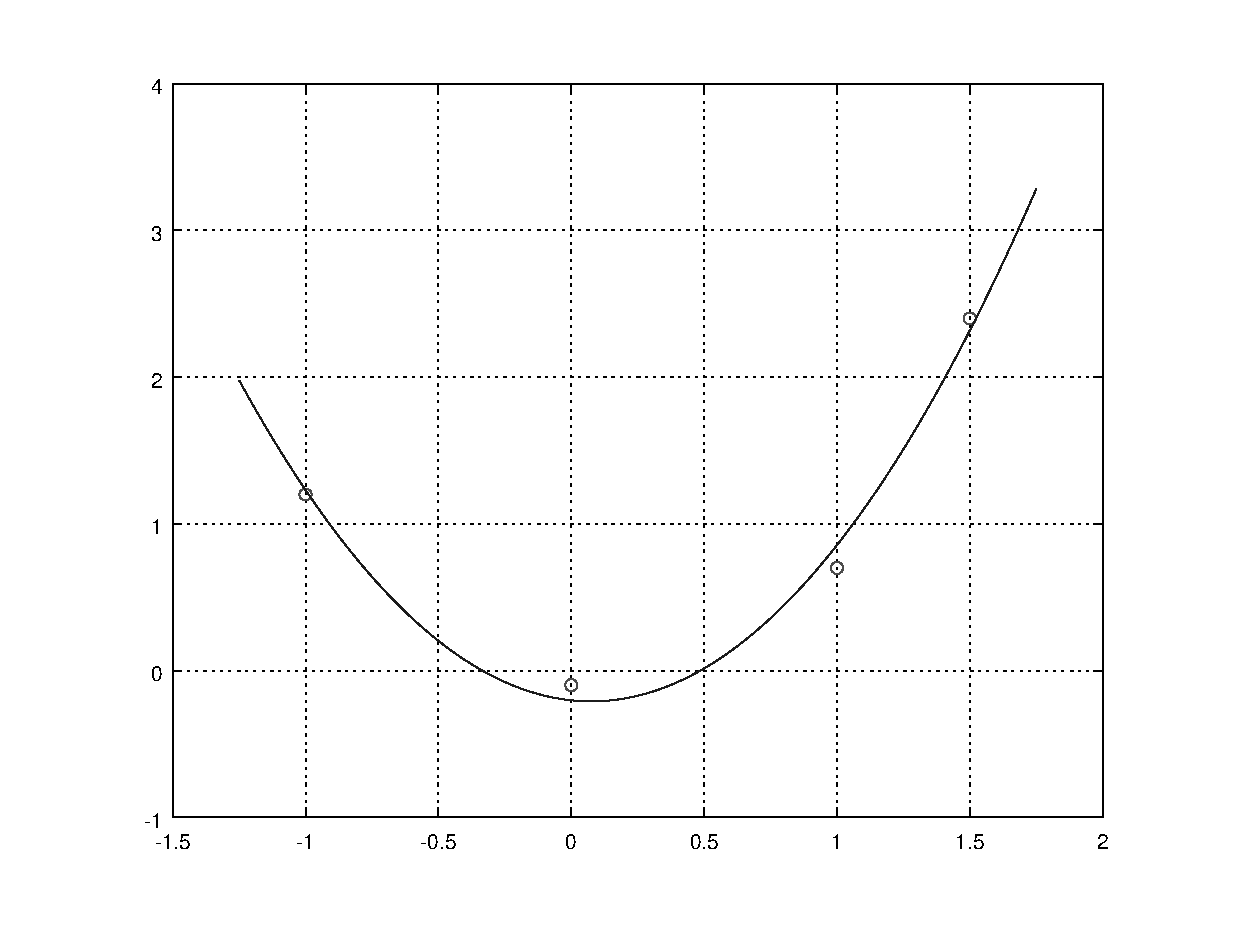
\includegraphics[width=\textwidth]{cap_ajuste/dados/ex_mq_poli/ex_mq_poli}
    \caption{Esboço do polinômio ajustado no Exemplo~\ref{ex:ajuste_de_polinomios}.}
    \label{fig:ex_mq_poli}
  \end{figure}
  
  
  Neste caso, a família de funções do problema de mínimos quadrados é $f_1(x) = x^2$, $f_2(x) = x$ e $f_3(x) = 1$. Assim sendo, os coeficientes $p = (p_1, p_2, p_3)$ são solução do seguinte sistema linear
  \begin{equation}\label{eq:aux3_md}
    A^TAp = A^Ty,
  \end{equation}
  onde $y = (y_1, y_2, y_3)$ e
  \begin{equation}
    A :=
    \begin{bmatrix}
      x_1^2 & x_1 & 1 \\
      x_2^2 & x_2 & 1 \\
      x_3^2 & x_3 & 1 \\
      x_4^2 & x_4 & 1
    \end{bmatrix}.
  \end{equation}
  Emfim, resolvendo as equações normais~\eqref{eq:aux3_md}, obtemos
  \begin{equation}
    p(x) = 1,25x^2 -0,188x - 0,203.
  \end{equation}
  A Figura~\ref{fig:ex_mq_poli} mostra um esboço dos pontos (em vermelho) e do polinômio ajustado (em azul).
  
  \ifisoctave
  Os coeficientes e um esboço do polinômio ajustado podem ser obtidos no \verb+GNU Octave+ com o seguinte código:
\begin{verbatim}
#pontos
x = [-1 0 1 1.5]';
y = [1.2, -0.1, 0.7, 2.4]';

#resol. as eqs. normais
A = [x.^2 x.^1 x.^0];
p = inv(A'*A)*A'*y

#esboco do pol. ajustado
xx = linspace(-1.25,1.75);
plot(x,y,'ro',...
     xx,polyval(p,xx));grid
\end{verbatim}
  \fi
  
\end{ex}


\begin{ex}\normalfont{(Ajuste de curvas)}\label{ex:ajuste_de_curvas}
  Consideremos o mesmo conjunto de pontos do exemplo anterior (Exemplo~\ref{ex:ajuste_de_polinomios}). Aqui, vamos ajustar uma curva da forma
  \begin{equation}
    f(x) = c_1\sen(x) + c_2\cos(x) + c_3
  \end{equation}
no sentido de mínimos quadrados. Para tanto, formamos a matriz
\begin{equation}
  A :=
  \begin{bmatrix}
    \sen(x_1) & \cos(x_1) & 1 \\
    \sen(x_2) & \cos(x_2) & 1 \\
    \sen(x_3) & \cos(x_3) & 1 \\
    \sen(x_4) & \cos(x_4) & 1
  \end{bmatrix}
\end{equation}
  e, então, resolvemos as equações normais $A^TAc = A^Ty$ para o vetor de coeficientes $c=(c_1, c_2)$. Fazendo isso, obtemos $c_1=-0,198$, $c_2=-2,906$ e $c_3=2,662$. A Figura~\ref{fig:ex_ajuste_de_curvas} mostra um esboço da curva ajustada (linha azul) aos pontos dados (círculos vermelhos).

  \begin{figure}[h]
    \centering
    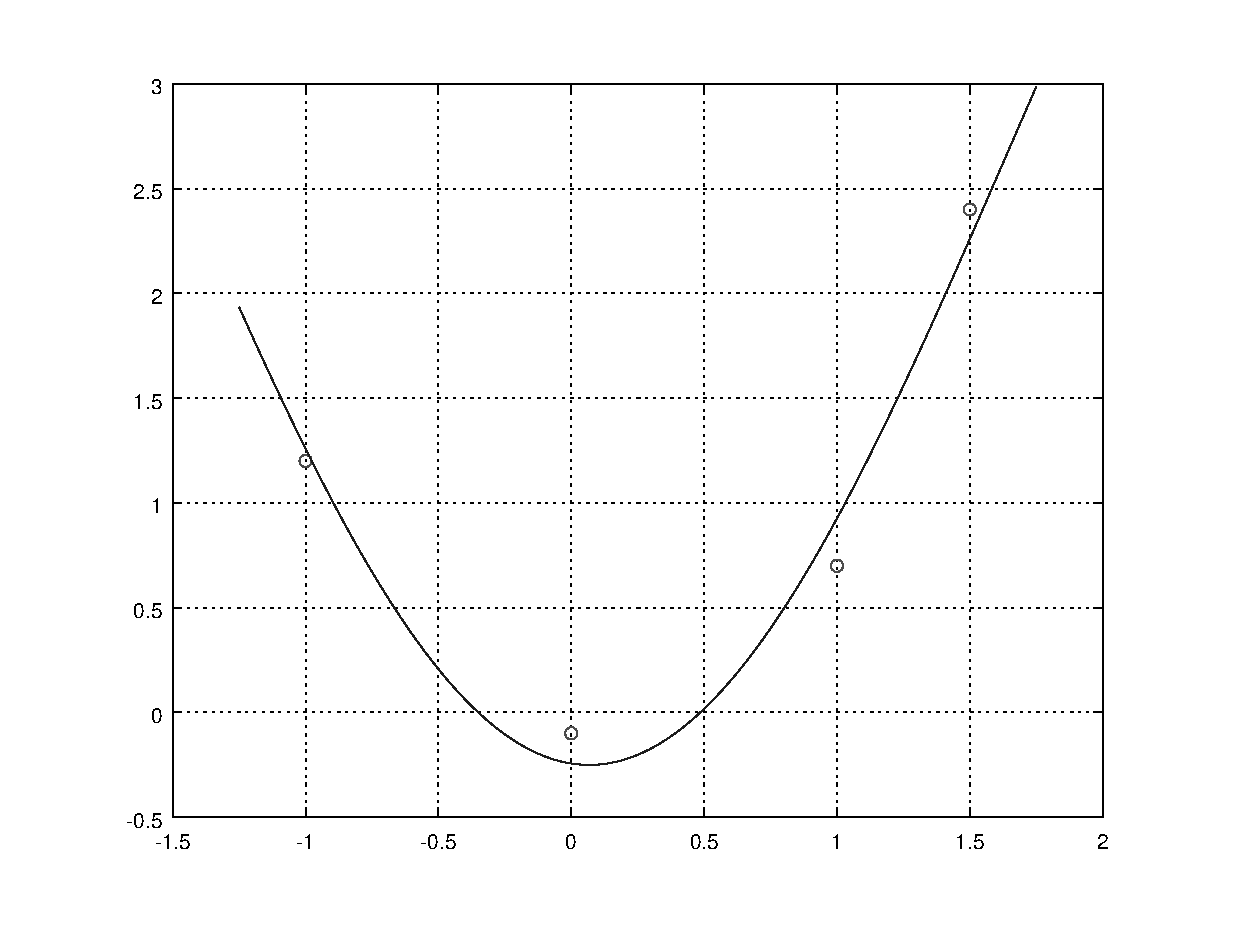
\includegraphics[width=\textwidth]{cap_ajuste/dados/ex_mq_curvas/ex_mq_curvas}
    \caption{Esboço da curva ajustada no Exemplo~\ref{ex:ajuste_de_curvas}.}
    \label{fig:ex_ajuste_de_curvas}
  \end{figure}

\ifisoctave
Os coeficientes e um esboço do polinômio ajustado podem ser obtidos no \verb+GNU Octave+ com o seguinte código:
\begin{verbatim}
#pontos
x = [-1 0 1 1.5]';
y = [1.2, -0.1, 0.7, 2.4]';

#resol. as eqs. normais
A = [sin(x) cos(x) ones(4,1)];
c = inv(A'*A)*A'*y

#curva ajustada
f = @(x) c(1)*sin(x) + c(2)*cos(x) + c(3)

#esboco da fun. ajustada
xx = linspace(-1.25,1.75);
plot(x,y,'ro',...
     xx,f(xx));grid
\end{verbatim}
\fi

\end{ex}

\begin{ex}\normalfont{(Um problema não linear)}\label{ex:mq_nlin0}
  Consideremos o problema de ajustar, no sentido de mínimos quadrados, à função
  \begin{equation}
    f(x) = c_1e^{c_2x}
  \end{equation}
ao seguinte conjunto de pontos
\begin{center}
  \begin{tabular}{l|rrrr}
    $i$ & $1$ & $2$ & $3$ & $4$ \\\hline
    $x_i$ & $-1$ & $0$ & $1$ & $1,5$\\
    $y_i$ & $8,0$ & $1,5$ & $0,2$ & $0,1$\\\hline
  \end{tabular}
\end{center}

Aqui, temos um problema não linear de mínimos quadrados que pode ser transformado em um problema linear fazendo-se
\begin{align}
  y = c_1e^{c_2x} &\Rightarrow \ln y = \ln c_1e^{c_2x}\\
                  &\Rightarrow \ln y = \ln c_1 + c_2x.
\end{align}
Isto é, denotando $d_1 := \ln c_1$ e $d_2 := c_2$, o problema se resume a ajustar uma reta $r(x) = d_1 + d_2x$ ao conjunto de pontos $\{(x_i, \ln y_i)\}_{i=1}^4$. 

Para resolver o problema transformado, formamos a matriz
\begin{equation}
  A :=
  \begin{bmatrix}
    1 & x_1 \\
    1 & x_2 \\
    1 & x_3 \\
    1 & x_4
  \end{bmatrix}
\end{equation}
e, então, resolvemos as equações normais $A^TAd = A^T\ln y$, com $\ln y = (\ln y_1, \ln y_2, \ln y_3, \ln y_4)$, donde obtemos $d_1=0,315$ e $d_2=-1,792$. Das definições de $d_1$ e $d_2$, temos $c_2 = d_2 = -1,792$ e $c_1 = e^{d_1} = 1,371$. A Figura~\ref{fig:ex_mq_nlin0} mostra um esboço da curva $f(x) = c_1e^{c_2x}$ ajustada (linha azul) aos pontos dados (círculos vermelhos).

\begin{figure}[h]
  \centering
  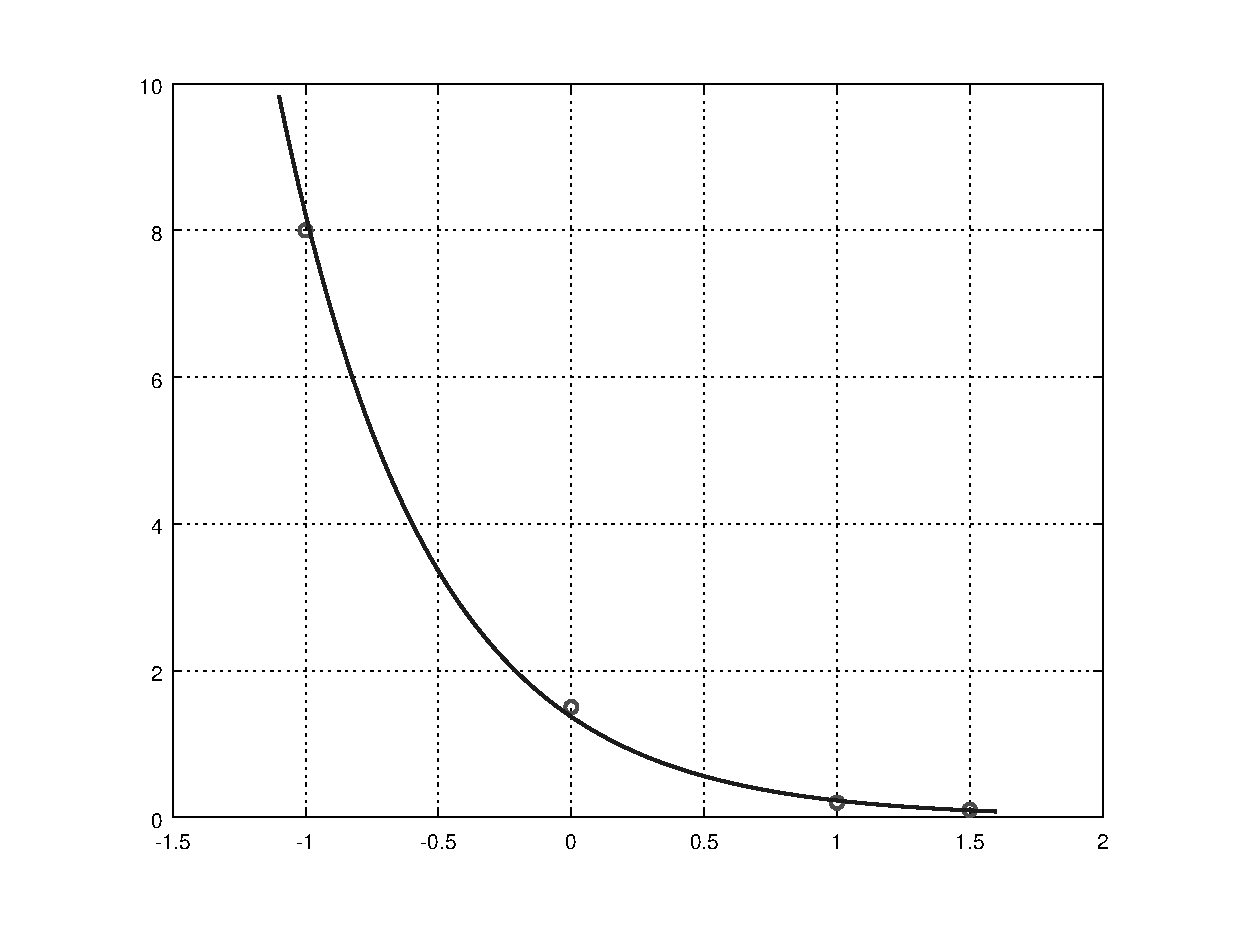
\includegraphics[width=\textwidth]{cap_ajuste/dados/ex_mq_nlin0/ex_mq_nlin0}
  \caption{Esboço da curva ajustada no Exemplo~\ref{ex:mq_nlin0}.}
  \label{fig:ex_mq_nlin0}
\end{figure}

\ifisoctave
O ajuste e um esboço da função ajustada podem ser feitos no \verb+GNU Octave+ com o seguinte código:
\begin{verbatim}
#pontos
x = [-1 0 1 1.5]';
y = [8.0 1.5 0.2 0.1]';

#resol. as eqs. normais
A = [ones(4,1) x];
d = inv(A'*A)*A'*log(y)

#fun. ajustada
c = [exp(d(1)); d(2)]
f = @(x) c(1)*exp(c(2)*x);

#esboco da fun. ajustada
xx = linspace(-1.1,1.6);
plot(x,y,'ro','linewidth',1.5,...
     xx,f(xx),'b-','linewidth',1.5);grid
\end{verbatim}
\fi

\end{ex}

\subsection*{Exercícios}

\begin{exer}\label{exer:mq_reta}
  Determine a reta $y = c_1x + c_2$ que melhor se ajusta, no sentido de mínimos quadrados, aos pontos
  \begin{center}
    \begin{tabular}{l|ccccc}
      $i$ & $1$ & $2$ & $3$ & $4$ & $5$ \\\hline
      $x_i$ & $-2,5$ & $-1,3$ & $0,2$ & $1,7$ & $2,3$\\
      $y_i$ & $3,8$ & $1,5$ & $-0,7$ & $-1,5$ & $-3,2$\\\hline
    \end{tabular}
  \end{center}
Por fim, compute a norma $L^2$ do resíduo, i.e. $\|r(c)\|_2 = \|y - (c_1x - c_2)\|_2$ para os pontos dados.
\end{exer}
\begin{resp}
  \ifisoctave 
  \href{https://github.com/phkonzen/notas/blob/master/src/MatematicaNumerica/cap_ajuste/dados/exer_mq_reta/exer_mq_reta.m}{Código.} 
  \fi
  $c_1 = -1,3259$, $c_2 = 8,66071\E-2$, $\|r(c)\|_2 = 1,01390$.
\end{resp}

\begin{exer}\label{exer:mq_poli}
  Determine o polinômio $y = c_1x^3 + c_2x^2 + c_3x + c_4$ que melhor se ajusta, no sentido de mínimos quadrados, aos pontos
  \begin{center}
    \begin{tabular}{l|ccccc}
      $i$ & $1$ & $2$ & $3$ & $4$ & $5$ \\\hline
      $x_i$ & $-2,5$ & $-1,3$ & $0,2$ & $1,7$ & $2,3$\\
      $y_i$ & $3,8$ & $0,5$ & $2,7$ & $1,2$ & $-1,3$\\\hline
    \end{tabular}
  \end{center}
Por fim, compute a norma $L^2$ do resíduo, i.e. $\|r(c)\|_2$.
\end{exer}
\begin{resp}
  \ifisoctave 
  \href{https://github.com/phkonzen/notas/blob/master/src/MatematicaNumerica/cap_ajuste/dados/exer_mq_poli/exer_mq_poli.m}{Código.} 
  \fi
  $c_1 = -4,50361\E-1$, $c_2 = -2,78350\E-1$, $c_3 = 1,46291$, $c_4 = 2,09648$, $\|r(c)\|_2 = 5,71346$
\end{resp}

\begin{exer}\label{exer:mq_curva}
  Determine a curva $y = c_1\sen x + c_2\cos x + c_3$ que melhor se ajusta, no sentido de mínimos quadrados, aos pontos
  \begin{center}
    \begin{tabular}{l|ccccc}
      $i$ & $1$ & $2$ & $3$ & $4$ & $5$ \\\hline
      $x_i$ & $-2,5$ & $-1,3$ & $0,2$ & $1,7$ & $2,3$\\
      $y_i$ & $3,8$ & $0,5$ & $2,7$ & $1,2$ & $-1,3$\\\hline
    \end{tabular}
  \end{center}
Por fim, compute a norma $L^2$ do resíduo, i.e. $\|r(c)\|_2$.
\end{exer}
\begin{resp}
  \ifisoctave 
  \href{https://github.com/phkonzen/notas/blob/master/src/MatematicaNumerica/cap_ajuste/dados/exer_mq_curva/exer_mq_curva.m}{Código.} 
  \fi
  $c_1 = -2,76842$, $c_2 = -7,17935\E-1$, $c_3 = 1,37014\E-1$, $\|r(c)\|_2 = 2,48880\E+1$
\end{resp}

\begin{exer}\label{exer:mq_nlin0}
  Use a transformação $z = \ln y$ para ajustar, no sentido de mínimos quadrados, a curva $y = c_1e^{c_2(x-c_3)^2}$ aos pontos
  \begin{center}
    \begin{tabular}{l|cccccc}
      $i$ & $1$ & $2$ & $3$ & $4$ & $5$ & $6$ \\\hline
      $x_i$ & $-0,5$ & $0,5$ & $1,3$ & $2,1$ & $2,7$ & $3,1$ \\
      $y_i$ & $0,1$ & $1,2$ & $2,7$ & $0,9$ & $0,2$ & $0,1$ \\\hline
    \end{tabular}
  \end{center}
\end{exer}
\begin{resp}
  \ifisoctave 
  \href{https://github.com/phkonzen/notas/blob/master/src/MatematicaNumerica/cap_ajuste/dados/exer_mq_nlin0/exer_mq_nlin0.m}{Código.} 
  \fi
  $c_1 = 2,10131\E+0$, $c_2 = -9,73859\E-1$, $c_3 = 1.25521\E+0$
\end{resp}
   
\section{Problemas não lineares}\label{cap_ajuste_sec_prob_nlin}

Um problema não linear de mínimos quadrados consiste em ajustar uma dada função $f(x;c)$ que dependa não linearmente dos parâmetros $c = (c_1, c_2, \dotsc, c_m)$, $m\geq 1$, a um dado conjunto de $n\geq m$ pontos $\{(x_i, y_i)\}_{i=1}^n$. Mais especificamente, buscamos resolver o seguinte problema de minimização
\begin{equation}\label{eq:prob_nlin_mq}
  \min_{\{c_1, c_2, \dotsc, c_m\}} \left[E := \sum_{i=1}^n \left(y_i - f(x_i;c)\right)^2\right].
\end{equation}
Aqui, denotaremos por $r(c) := (r_1(c), r_2(c), \dotsc, r_n(c))$ o vetor dos resíduos $r_i(c) := y_i - f(x_i,c)$. Com isso, o problema se resume a encontrar o vetor de parâmetros $c$ que minimiza
\begin{equation}
  E = \|r(c)\|_2^2.
\end{equation}
Tais parâmetros são solução do seguinte sistema de equações
\begin{equation}
  \frac{\p E}{\p c_j} = 2\sum_{i=1}^n r_i(c)\frac{\p}{\p c_j}r_i(c) = 0
\end{equation}
ou, equivalentemente, da equação
\begin{equation}\label{eq:grad_E}
  \nabla E = 0 \Leftrightarrow J_R^T(c)r(c) = 0,
\end{equation}
onde
\begin{equation}
  J_R(c) :=
  \begin{bmatrix}
    \frac{\p r_1}{\p c_1} & \frac{\p r_1}{\p c_2} & \cdots & \frac{\p r_1}{\p c_m}\\
    \frac{\p r_2}{\p c_1} & \frac{\p r_2}{\p c_2} & \cdots & \frac{\p r_2}{\p c_m}\\
    \vdots  & \vdots & \vdots & \vdots \\
    \frac{\p r_n}{\p c_1} & \frac{\p r_n}{\p c_2} & \cdots & \frac{\p r_n}{\p c_m}
  \end{bmatrix}
\end{equation}
é a jacobiana do resíduo $r$ em relação aos parâmetros $c$.

Podemos usar o método de Newton para resolver~\eqref{eq:grad_E}. Para tanto, escolhemos uma aproximação inicial para $c^{(1)} = (c_1^{(1)}, c_2^{(1)}, \dotsc, c_m^{(1)})$ e iteramos
\begin{align}
  H_R(c^{(k)})\delta^{(k)} &= -J_R^T(c)r(c) \label{eq:mqnl_newton1}\\
  c^{(k+1)} &= c^{(k)} + \delta^{(k)} \label{eq:mqnl_newton2},
\end{align}
onde $\delta^{(k)} = (\delta_1^{(k)}, \delta_2^{(k)}, \delta_m^{(k)})$ é a atualização de Newton (ou direção de busca) e $H_R(c) := [h_{p,q}(c)]_{p,q=1}^{m,m}$ é a matriz hessiana, cujos elementos são
\begin{equation}
  h_{p,q} := \sum_{i=1}^n\left\{\frac{\p r_i}{\p c_q}\frac{\p r_i}{\p c_p} + r_i\frac{\p^2 r_i}{\p c_q\p c_p}\right\}.
\end{equation}

\begin{ex}\label{ex:mqnl_newton}
  Consideremos o problema de ajustar, no sentido de mínimos quadrados, a função
  \begin{equation}
    f(x;c) = c_1e^{c_2x}
  \end{equation}
ao seguinte conjunto de pontos
\begin{center}
  \begin{tabular}{l|rrrr}
    $i$ & $1$ & $2$ & $3$ & $4$ \\\hline
    $x_i$ & $-1$ & $0$ & $1$ & $1,5$\\
    $y_i$ & $8,0$ & $1,5$ & $0,2$ & $0,1$\\\hline
  \end{tabular}
\end{center}

Aqui, vamos utilizar a iteração de Newton para o problema de mínimos quadrados, i.e. a iteração dada em \eqref{eq:mqnl_newton1}-\eqref{eq:mqnl_newton2}. Para tanto, para cada $i=1, 2, 3, 4$, precisamos das seguintes derivadas parciais do resíduo $r_i(c) := y_i - c_1e^{c_2x_i}$:
\begin{align}
  &\frac{\p}{\p c_1}r_i(c) = - e^{c_2x_i},\\
  &\frac{\p}{\p c_2}r_i(c) = - c_1x_ie^{c_2x_i},\\
  &\frac{\p^2}{\p c_1^2}r_i(c) = 0,\\
  &\frac{\p^2}{\p c_1\p c_2}r_i(c) = \frac{\p^2}{\p c_2\p c_1}r_i(c) = - x_ie^{c_2x_i},\\
  &\frac{\p^2}{\p c_2^2}r_i(c) = - c_1x_i^2e^{c_2x_i}.
\end{align}

\begin{figure}[h]
  \centering
  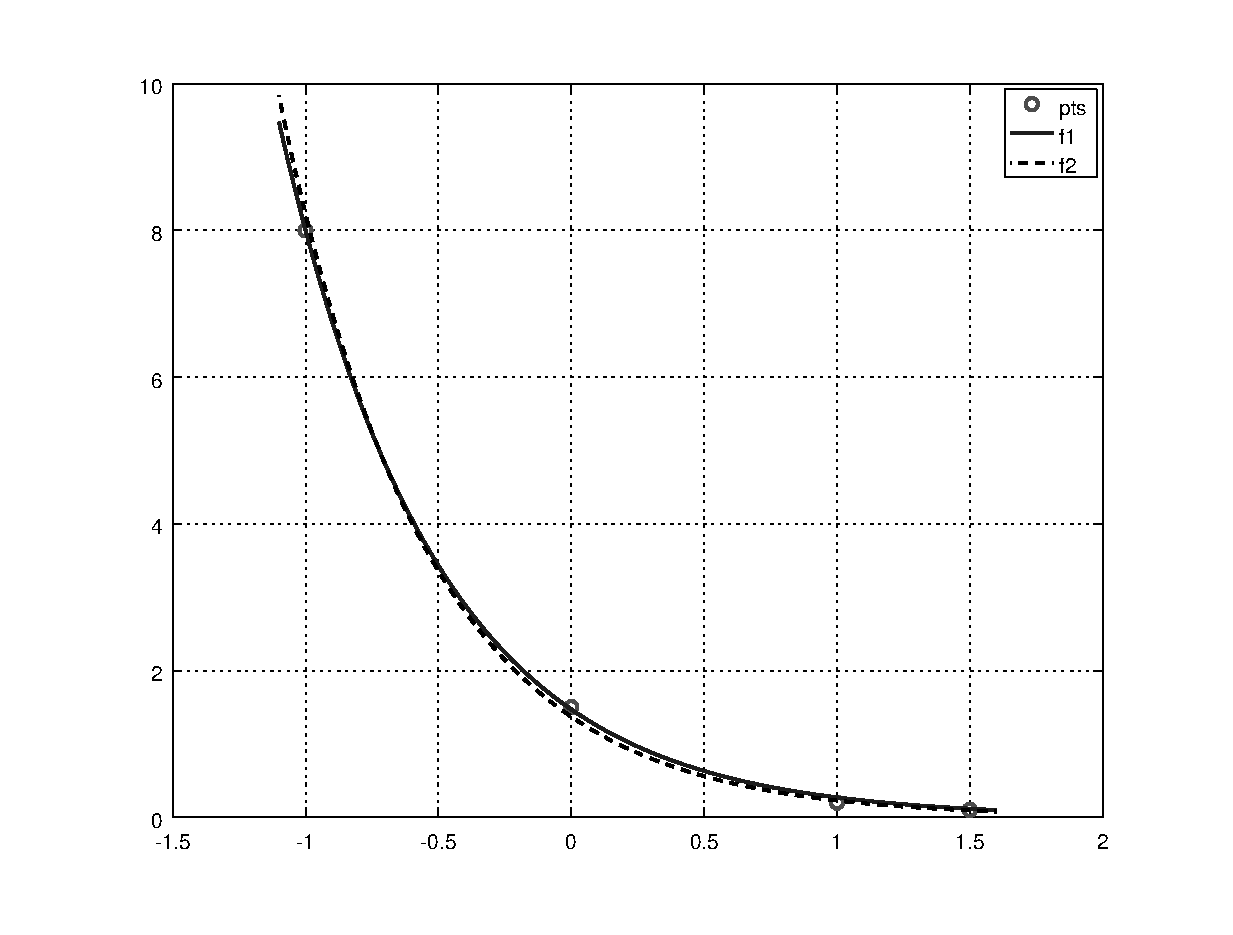
\includegraphics[width=\textwidth]{cap_ajuste/dados/ex_mqnl_N/ex_mqnl_N}
  \caption{Esboço da curva ajustada no Exemplo~\ref{ex:mqnl_newton}.}
  \label{fig:ex_mqnl_newton}
\end{figure}

Com isso e tomando $c^{(1)} = (1,4, ~-1,8)$ (motivado do Exemplo~\ref{ex:mq_nlin0}), computamos as iterações de Newton~\eqref{eq:mqnl_newton1}-\eqref{eq:mqnl_newton2}. Iterando até a precisão de $TOL = 10^{-4}$, obtemos a solução $c_1 = 1,471$ e $c_2 = -1,6938$. Na Figura~\ref{fig:ex_mqnl_newton} vemos uma comparação entre a curva aqui ajustada ($-$) e aquela obtida no Exemplo~\ref{ex:mq_nlin0} ($--$).

\ifisoctave
O ajuste discutido neste exemplo pode ser computado no \verb+GNU Octave+ com o seguinte código:
\begin{verbatim}
#pontos
global x = [-1 0 1 1.5]';
global y = [8.0 1.5 0.2 0.1]';

#fun. objetivo
f = @(x,c) c(1)*exp(c(2)*x);

#residuo
r = @(c) y - f(x,c);

#jacobiana
function A = J(c)
  global x
  A = zeros(4,2);
  A(:,1) = - exp(c(2)*x);
  A(:,2) = - c(1)*x.*exp(c(2)*x);
endfunction

#hessiana
function A = H(c)
  global x
  global y
  A = zeros(2,2);
  A = J(c)'*J(c);
  for i=1:4
    A(1,1) += 0;
    A(1,2) += (y(i) - c(1)*exp(c(2)*x(i))) * ...
              (- x(i)*exp(c(2)*x(i)));
    A(2,1) += (y(i) - c(1)*exp(c(2)*x(i))) * ...
              (- x(i)*exp(c(2)*x(i)));
    A(2,2) += (y(i) - c(1)*exp(c(2)*x(i))) * ...
              (- c(1)*x(i)^2*exp(c(2)*x(i)));
  endfor
endfunction

#aprox. inicial
c = [1.4 -1.8]';

#iteracoes de Newton
k=0;
do
  k+=1;
  delta = - inv(H(c))*J(c)'*r(c);
  c = c + delta;
  [k,c',norm(delta)]
until ((k>10) | (norm(delta)<1e-4))
\end{verbatim}
\fi
\end{ex}

Observamos que a solução obtida no exemplo anterior (Exemplo~\ref{ex:mqnl_newton}) difere da previamente encontrada no Exemplo~\ref{ex:mq_nlin0}. Naquele exemplo, os parâmetros obtidos nos fornecem $E = 6,8\E-2$, enquanto que a solução do exemplo anterior fornece $E = 6,1\E-3$. Isto é esperado, pois naquele exemplo resolvemos um problema aproximado, enquanto no exemplo anterior resolvemos o problema por si.

O emprego do método de Newton para o problema de mínimos quadrados tem a vantagem da taxa de convergência quadrática, entretanto requer a computação das derivadas parciais de segunda ordem do resíduo. Na sequência discutimos alternativas comumente empregadas.

\subsection{Método de Gauss-Newton}

O método de Gauss-Newton é uma técnica iterativa que aproxima o problema não linear de mínimos quadrados \eqref{eq:prob_nlin_mq} por uma sequência de problemas lineares. Para seu desenvolvimento, começamos de uma aproximação inicial $c^{(1)} = (c_1^{(1)}, c_2^{(1)}, \dotsc, c_m^{(1)})$ dos parâmetros que queremos ajustar. Também, assumindo que a $n$-ésima iterada $c^{(k)}$ é conhecida, faremos uso da aproximação de primeira ordem de $f(x,c)$ por polinômio de Taylor, i.e.
\begin{equation}
  f(x;c^{(k+1)}) \approx f(x;c^{(k)}) + \nabla_c f(x;c^{(k)})(c^{(k+1)}-c^{(k)}),
\end{equation}
onde
\begin{equation}
  \nabla_c f(x;c) = \left[\frac{\p}{\p c_1}f(x;c) ~\frac{\p}{\p c_2}f(x;c) ~\cdots ~\frac{\p}{\p c_m}f(x;c)\right].
\end{equation}

O método consiste em obter a solução do problema não linear \eqref{eq:prob_nlin_mq} pelo limite dos seguintes problemas lineares de mínimos quadrados
\begin{align}
  \min_{\delta^{(k)}} &\left[\tilde{E} := \sum_{i=1}^n (y_i - f(x_i,c^{(k)}) - \nabla_c f(x_i;c^{(k)})\delta^{(k)})^2\right] \label{eq:mq_gn0}\\
  &c^{(k+1)} = c^{(k)} + \delta^{(k)}.
\end{align}

Agora, usando a notação de resíduo $r(c) = y - f(x;c)$, observamos que \eqref{eq:mq_gn0} consiste no problema linear de mínimos quadrados
\begin{equation}
  \min_{\delta^{(k)}} \|r(c^{(k)}) + J_R(c^{(k)})\delta^{(k)}\|_2^2,
\end{equation}
o qual é equivalente a resolver as equações normais
\begin{equation}
  J_R^T(c^{(n)})J_R(c^{(n)})\delta^{(n)} = -J_R^T(c)r(c).
\end{equation}

Com isso, dada uma aproximação inicial $c^{(1)}$, a \emph{iteração do método de Gauss-Newton} consiste em
\begin{align}
  &J_R^T(c^{(k)})J_R(c^{(k)})\delta^{(k)} = -J_R^T(c)r(c)\\
  &c^{(k+1)} = c^{(k)} + \delta^{(k)}.
\end{align}

\begin{ex}
  A aplicação da iteração de Gauss-Newton ao problema de mínimos quadrados discutido no Exemplo~\ref{ex:mqnl_newton} nos fornece a mesma solução obtida naquele exemplo (preservadas a aproximação inicial e a tolerância de precisão).

\ifisoctave
A implementação do método de Gauss-Newton para este problema no \verb+GNU Octave+ pode ser feita com o seguinte código:
\begin{verbatim}
#pontos
global x = [-1 0 1 1.5]';
y = [8.0 1.5 0.2 0.1]';

#fun. objetivo
f = @(x,c) c(1)*exp(c(2)*x);

#residuo
r = @(c) y - f(x,c);

#jacobiana
function A = J(c)
  global x
  A = zeros(4,2);
  A(:,1) = - exp(c(2)*x);
  A(:,2) = - c(1)*x.*exp(c(2)*x);
endfunction

#aprox. inicial
c = [1.4 -1.8]';

#iteracoes de Gauss-Newton
k=0;
do
  k+=1;
  delta = - inv(J(c)'*J(c))*J(c)'*r(c);
  c = c + delta;
  [k,c',norm(delta)]
until ((k>10) | (norm(delta)<1e-4))
\end{verbatim}
\fi
\end{ex}

O método de Gauss-Newton pode ser lentamente convergente para problemas muito não lineares ou com resíduos grandes. Nesse caso, métodos de Gauss-Newton com amortecimento são alternativas robustas~\cite{Bjorck1996a,Nocedal2006a}. Na sequência, introduziremos um destes métodos, conhecido como método de Levenberg-Marquardt.

\subsection{Método de Levenberg-Marquardt}

O método de Levenberg-Marquardt é uma variação do método de Gauss-Newton no qual a direção de busca $\delta^{(n)}$ é obtida da solução do seguinte problema regularizado
\begin{equation} \label{eq:mq_gn0}
  \min_{\delta^{(k)}} \{\|r(c^{(k)}) + J_R(c^{(k)})\delta^{(k)}\|_2^2 + \mu^{(k)}\|\delta^{(k)}\|_2^2\}
\end{equation}
ou, equivalentemente,
\begin{equation} \label{eq:mq_gn0}
  \min_{\delta^{(k)}} \left\|
    \begin{bmatrix}
      r(c^{(k)})\\
      0
    \end{bmatrix} +
    \begin{bmatrix}
      J_R(c^{(k)})\\
      \mu^{(k)}I
    \end{bmatrix}
    \delta^{(k)}\right\|_2^2
\end{equation}

A taxa de convergência das iterações de Levenberg-Marquardt é sensível a escolha do parâmetro $\mu^{(k)}\geq 0$. Aqui, faremos esta escolha por tentativa e erro. O leitor pode aprofundar-se mais sobre esta questão na literatura especializada (veja, por exemplo, \cite{Bjorck1996a,Nocedal2006a}).

\begin{obs}
  Quando $\mu^{(k)} \equiv 0$ para todo $n$, o método de Levenberg-Marquardt é equivalente ao método de Gauss-Newton.
\end{obs}

\begin{ex}\label{ex:mqnl_LM}
  Consideremos o problema de mínimos quadrados discutido no Exemplo~\ref{ex:mqnl_newton}. O método de Gauss-Newton falha para este problema se escolhermos, por exemplo, $c^{(1)} = (0, 0)$. Isto ocorre pois, para esta escolha de $c^{(1)}$, a jacobiana $J(c^{(1)})$ não tem posto completo. Entretanto, o método de Levenberg-Marquardt com $\mu^{(k)} = 0,1$ é convergente, mesmo para esta escolha de $c^{(1)}$.

\ifisoctave
A implementação no \verb+GNU Octave+ do método de Levenberg-Marquardt (com $\mu^{(k)}=0,1$ constante) para este problema pode ser feita com o seguinte código:
\begin{verbatim}
#pontos
global x = [-1 0 1 1.5]';
y = [8.0 1.5 0.2 0.1]';

#fun. objetivo
f = @(x,c) c(1)*exp(c(2)*x);

#residuo
r = @(c) y - f(x,c);

#jacobiana
function A = JR(c)
  global x;
  A = zeros(4,2);
  A(:,1) = - exp(c(2)*x);
  A(:,2) = - c(1)*x.*exp(c(2)*x);
endfunction

#aprox. inicial
c = [0 0]';

#param. de amortecimento
mu = 0.1;

#iteracoes de Gauss-Newton
k=0;
do
  k+=1;
  JJ = [JR(c);mu*eye(2,2)];
  delta = - inv(JJ'*JJ)*JJ'*[r(c);zeros(2,1)];
  c = c + delta;
  printf("%d %1.1e %1.3e %1.3e\n", k,norm(delta),c')
until ((k>10) | (norm(delta)<1e-4))
\end{verbatim}
\fi
\end{ex}

\subsection*{Exercícios}

\begin{exer}\label{exer:mqnl_GN}
  Use o método de Gauss-Newton para ajustar, no sentido de mínimos quadrados e com precisão de $10^{-4}$, a curva $y = c_1e^{c_2(x-c_3)^2}$ aos pontos
  \begin{center}
    \begin{tabular}{l|cccccc}
      $i$ & $1$ & $2$ & $3$ & $4$ & $5$ & $6$ \\\hline
      $x_i$ & $-0,5$ & $0,5$ & $1,3$ & $2,1$ & $2,7$ & $3,1$ \\
      $y_i$ & $0,1$ & $1,2$ & $2,7$ & $0,9$ & $0,2$ & $0,1$ \\\hline
    \end{tabular}
  \end{center}
Use as condições iniciais:
\begin{enumerate}[a)]
\item $c_1 = 2,1$, $c_2=-1$ e $c_3=1,3$.
\item $c_1=1$, $c_2=-1$ e $c_3=-1$.
\end{enumerate}
\end{exer}
\begin{resp}
  \ifisoctave 
  \href{https://github.com/phkonzen/notas/blob/master/src/MatematicaNumerica/cap_ajuste/dados/exer_mqnl_GN/exer_mqnl_GN.m}{Código.} 
  \fi
  a) $c_1 = 2,69971\E+0$, $c_2 = -1,44723\E+0$, $c_3 = 1.24333\E+0$; b) divergente.
\end{resp}

\begin{exer}
  Resolva o exercício anterior (Exercício~\ref{exer:mqnl_GN}) usando o método de Levenberg-Marquardt com amortecimento constante $\mu=0,2$.
\end{exer}
\begin{resp}
  \ifisoctave 
  \href{https://github.com/phkonzen/notas/blob/master/src/MatematicaNumerica/cap_ajuste/dados/exer_mqnl_LM/exer_mqnl_LM.m}{Código.} 
  \fi
  a)  $c_1 = 2,69971\E+0$, $c_2 = -1,44723\E+0$, $c_3 = 1.24333\E+0$; b) $c_1 = 2,69971\E+0$, $c_2 = -1,44723\E+0$, $c_3 = 1.24333\E+0$
\end{resp}

%Este trabalho está licenciado sob a Licença Atribuição-CompartilhaIgual 4.0 Internacional Creative Commons. Para visualizar uma cópia desta licença, visite http://creativecommons.org/licenses/by-sa/4.0/deed.pt_BR ou mande uma carta para Creative Commons, PO Box 1866, Mountain View, CA 94042, USA.

\chapter{Derivadas}\label{cap_deriv}
\thispagestyle{fancy}

\ifispython
\begin{obs}\normalfont{(Códigos \verb+Python+)}\label{obs:deriv_python}
  Nos códigos \verb+Python+ inseridos ao longo deste capítulos, estaremos assumindo o seguinte preâmbulo:
\begin{verbatim}
%matplotlib inline
from sympy import *
init_printing()
var('x',real=True)
\end{verbatim}
\end{obs}
\fi

\section{Retas tangentes e derivadas}\label{cap_deriv_sec_retg}

Definimos a {\bf reta secante} ao gráfico de uma dada função $f$ pelos pontos $x_0$ e $x_1$, $x_0\neq x_1$, como sendo a reta determinada pela equação
\begin{equation}
  y = \frac{f(x_1)-f(x_0)}{x_1-x_0}(x-x_0)+f(x_0).
\end{equation}
Isto é, é a reta que passa pelos pontos $(x_0,f(x_0))$ e $(x_1,f(x_1))$. Veja a Figura \ref{fig:retsectg}. Observemos que o coeficiente angular da reta secante é
\begin{equation}
  m_{\text{sec}} = \frac{f(x_1)-f(x_0)}{x_1-x_0}.
\end{equation}

\begin{figure}[H]
  \centering
  \includegraphics[width=0.7\textwidth]{./cap_deriv/dados/fig_retsectg/fig_retsectg}
  \caption{Esboços de uma reta secante (verde) e da reta tangente (vermelho) ao gráfico de uma função.}
  \label{fig:retsectg}
\end{figure}

A {\bf reta tangente} ao gráfico de uma função $f$ em $x=x_0$ é a reta que passa pelo ponto $(x_0, f(x_0))$ e tem coeficiente angular
\begin{equation}\label{eq:mtg}
  m_{\text{tg}} = \lim_{x_1\to x_0} \frac{f(x_1)-f(x_0)}{x_1-x_0}.
\end{equation}
Isto é, a reta de equação
\begin{equation}
  y = m_{\text{tg}}(x-x_0)+f(x_0).
\end{equation}
Menos formal, é a reta limite das retas secantes ao gráfico da função pelos pontos $x_0$ e $x_1$, quando $x_1\to x_0$. Veja a Figura \ref{fig:retsectg}.

\begin{obs}
  Fazendo $h = x_1-x_0$, temos que \eqref{eq:mtg} é equivalente a
  \begin{equation}
    m_{\text{tg}} = \lim_{h\to 0} \frac{f(x_0+h)-f(x_0)}{h}.
  \end{equation}
\end{obs}

\begin{ex}
  Seja $f(x)=x^2$ e $x_0 = 1$. O coeficiente angular da reta tangente ao gráfico de $f$ no ponto $x_0$ é
  \begin{align}
    m_{\text{tg}} &= \lim_{h\to 0} \frac{f(x_0+h)-f(x_0)}{h}\\
                  &= \lim_{h\to 0} \frac{(1+h)^2-1}{h}\\
                  &= \lim_{h\to 0} \frac{1+2h+h^2-1}{h}\\
                  &= \lim_{h\to 0} \frac{2+h}{1} = 2.
  \end{align}
  Assim sendo, a reta tangente ao gráfico de $f(x)=x^2$ no ponto $x_0=1$ tem coeficiente angular $m_{\text{tg}} = 2$ e equação
  \begin{equation}
    y = 2(x-1)+1 = 2x-1.
  \end{equation}
  \ifispython
  Com o \verb+SymPy+, podemos obter a reta tangente com os seguintes comandos:
\begin{verbatim}
h = symbols('h',real=True)
f = lambda x: x**2
x0 = 1
# coef. angular
mtg = limit((f(x0+h)-f(x0))/h,h,0)

# reta tangente
mtg*(x-x0)+f(x0)
\end{verbatim}
  \fi
\end{ex}

\subsection{A derivada em um ponto}

A {\bf derivada} de uma função $f$ {\bf em um ponto} $x=x_0$ é denotada por $f'(x_0)$ ou $\displaystyle \frac{\dd f}{\dd x}(x_0)$ e é definida por
\begin{equation}
  f'(x_0) = \frac{\dd f}{\dd x}(x_0) = \lim_{h\to 0} \frac{f(x_0+h)-f(x_0)}{h}.
\end{equation}

\begin{ex}
  Vejamos os seguintes casos:
  \begin{enumerate}[a)]
  \item $f(x) = k$, $k$ constante.
    \begin{align}
      f'(x_0) &= \lim_{h\to 0} \frac{f(x_0+h)-f(x_0)}{h}\\
              &= \lim_{h\to 0} \frac{k-k}{h} = 0.
    \end{align}
  \item $f(x) = x$.
    \begin{align}
      f'(x_0) &= \lim_{h\to 0} \frac{f(x_0+h)-f(x_0)}{h} \\
              &= \lim_{h\to 0} \frac{x_0+h-x_0}{h} = 1.
    \end{align}
  \item $f(x) = \sqrt{x}$, $x_0=1$.
    \begin{align}
      f'(1) &= \lim_{h\to 0} \frac{\sqrt{1+h}-1}{h}\\
            &= \lim_{h\to 0} \frac{\sqrt{1+h}-1}{h}\frac{\sqrt{1+h}+1}{\sqrt{1+h}+1}\\
            &= \lim_{h\to 0} \frac{1+h-1}{h(\sqrt{1+h}+1)} = \frac{1}{2}.
    \end{align}
  \end{enumerate}
\end{ex}

\subsection*{Exercícios}

\emconstrucao

\section{Função derivada}\label{cap_deriv_sec_deriv}

A {\bf derivada} de uma função $f$ em relação à variável $x$ é a função $\displaystyle f' = \frac{\dd f}{\dd x}$ cujo valor em $x$ é
\begin{equation}\label{eq:derivada}
  \lim_{h\to 0} \frac{f(x+h)-f(x)}{h},
\end{equation}
quando este limite existe. Dizemos que $f$ é {\bf derivável} (ou {\bf diferenciável}) em um ponto $x$ de seu domínio, quando o limite dado em \eqref{eq:derivada} existe. Se isso ocorre para todo número real $x$, dizemos que $f$ é derivável em toda parte.

\begin{ex}
  A derivada de $f(x) = x^2$ é
  \begin{align}
    f'(x) &= \lim_{h\to 0} \frac{f(x+h)-f(x)}{h}\\
          &= \lim_{h\to 0} \frac{(x+h)^2 - x^2}{h}\\
          &= \lim_{h\to 0} \frac{x^2+2xh+h^2-x^2}{h}\\
          &= \lim_{h\to 0} 2x+h = 2x.
  \end{align}
  \ifispython
  Com o \verb+SymPy+, podemos usar os seguintes comandos para verificarmos este resultado:
\begin{verbatim}
h = symbols('h',real=True)
f = lambda x: x**2
limit((f(x+h)-f(x))/h,h,0)
\end{verbatim}
  \fi
\end{ex}

\begin{obs}
  A derivada à direita (à esquerda) de uma função $f$ em um ponto $x$ é definida por
  \begin{equation}
    f_{\pm}'(x) = \frac{\dd f}{\dd x^{\pm}} = \lim_{h\to 0^\pm} \frac{f(x+h)-f(x)}{h}.
  \end{equation}
  Desta forma, no caso de pontos extremos do domínio de uma função, empregamos a derivada lateral correspondente.
\end{obs}

\begin{ex}
  A função valor absoluto é derivável para todo $x\neq 0$ e não é derivável em $x=0$. De fato, para $x<0$ temos
  \begin{align}
    f'(x) &= \lim_{x\to 0} \frac{|x+h|-|x|}{h}\\
          &= \lim_{h\to 0} \frac{-(x+h)+x}{h}\\
          &= \lim_{h\to 0} \frac{h}{h} = 1.
  \end{align}
  Analogamente, para $x>0$ temos
  \begin{align}
    f'(x) &= \lim_{x\to 0} \frac{|x+h|-|x|}{h}\\
          &= \lim_{x\to 0} \frac{x+h-x}{h}\\
          &= \lim_{x\to 0} \frac{h}{h} = 1.
  \end{align}
  Agora, para $x=0$, devemos verificar as derivadas laterais:
  \begin{align}
    f'_+(0) &= \lim_{h\to 0^+} \frac{|h|-|0|}{h} = \lim_{h\to 0^+} \frac{h}{h} = 1,\\
    f'_-(0) &= \lim_{h\to 0^-} \frac{|h|-|0|}{h} = \lim_{h\to 0^-} \frac{-h}{h} = -1.
  \end{align}
  Como as derivadas laterais são diferentes, temos que $y = |x|$ não é derivável em $x=0$.
\end{ex}

\begin{ex}
  Vamos calcular a derivada de $f(x) = \sqrt{x}$. Para $x=0$, só faz sentido calcular a derivada lateral à direta:
  \begin{equation}
    f'(0) = \lim_{h\to 0^+} \frac{\sqrt{h}-\sqrt{0}}{h} = +\infty.
  \end{equation}
  Ou seja, $f(x) = \sqrt{x}$ não é derivável em $x=0$. Agora, para $x> 0$, temos
  \begin{align}
    f'(x) &= \lim_{h\to 0} \frac{\sqrt{x+h}-\sqrt{x}}{h}\\
          &= \lim_{h\to 0} \frac{\sqrt{x+h}-\sqrt{x}}{h}\frac{\sqrt{x+h}+\sqrt{x}}{\sqrt{x+h}+\sqrt{x}}\\
          &= \lim_{h\to 0} \frac{x+h-x}{h(\sqrt{x+h}+\sqrt{x})}\\
          &= \frac{1}{2\sqrt{x}}.
  \end{align}
\end{ex}

\subsection*{Exercícios}

\emconstrucao


\section{Regras básicas de derivação}\label{cap_deriv_sec_regras}

Vejamos as derivadas da função constante e da função potência.
\begin{itemize}
\item $\displaystyle \frac{\dd k}{\dd x} = 0$, onde $k$ é uma constante.

  Dem.: Com $f(x) \equiv k$ temos
  \begin{align}
    \frac{\dd k}{\dd x} &= \lim_{h\to 0} \frac{f(x+h)-f(x)}{h}\\
                        &= \lim_{h\to 0} \frac{k-k}{h} \\
                        &= \lim_{h\to 0} 0 = 0.
  \end{align}
  \ifispython
  No \verb+SymPy+, podemos usar os seguintes comandos para obtermos tal regra de derivação:
\begin{verbatim}
k = symbols('k',real=True)
diff(k,x)
\end{verbatim}
  \fi
  

\item $\displaystyle \frac{\dd x^n}{\dd x} = nx^{n-1}$, para $n$ inteiro positivo.

  Dem.: Com $f(x) = x^n$, temos
  \begin{align}
    \frac{\dd x^n}{\dd x} &= \lim_{h\to 0} \frac{f(x+h)-f(x)}{h}\\
                          &= \lim_{h\to 0} \frac{(x+h)^n-x^n}{h} \\
                          &= \lim_{h\to 0} \frac{x^n+nx^{n-1}h+\frac{n(n-1)}{2}x^{n-2}h^2 + \cdots +h^n-x^n}{h}\\
                          &= \lim_{h\to 0} nx^{n-1}+\frac{n(n-1)}{2}x^{n-2}h+\cdots+h^{n-1}\\
                          &= nx^{n-1}.
  \end{align}
  \ifispython
  No \verb+SymPy+, podemos usar os seguintes comandos para obtermos tal regra de derivação:
\begin{verbatim}
n = symbols('n',integer=True, positive=True)
simplify(diff(x**n,x))
\end{verbatim}
  \fi
\end{itemize}

\begin{ex}
  Vejamos os seguintes casos:
  \begin{enumerate}[a)]
  \item $\displaystyle \frac{\dd \sqrt{2}}{\dd x} = 0$.
  \item $\displaystyle \frac{\dd x^3}{\dd x} = 3x^2$.
  \end{enumerate}
\end{ex}

\subsection{Multiplicação por constante e soma}

Sejam $c$ um número real, $u$ e $v$ funções. Temos as seguintes regras básicas de derivação:
\begin{itemize}
\item $\displaystyle (cu)' = cu'$.

  Dem.:
  \begin{align}
    \frac{\dd}{\dd x}(cu)(x) &= \lim_{h\to 0} \frac{cu(x+h)-cu(x)}{h} \\
                          &= c\lim_{h\to 0} \frac{u(x+h)-u(x)}{h} \\
                          &= c\frac{\dd u}{\dd x}.
  \end{align}
  \ifispython
  No \verb+SymPy+, podemos usar os seguintes comandos para obtermos tal regra de derivação:
\begin{verbatim}
c = symbols('c', real=True)
u = Function('u', real=True)(x)
diff(c*u,x)
\end{verbatim}
  \fi

\item $\displaystyle (u\pm v)' = u'\pm v'$.

  Dem.:
  \begin{align}
    (u\pm v)'(x) &= \lim_{h\to 0} \frac{(u\pm v)(x+h)-(u\pm v)(x)}{h}\\
                              &= \lim_{h\to 0} \left[\frac{u(x+h)-u(x)}{h}\pm\frac{v(x+h)-v(x)}{h}\right]\\
              &= u'(x) \pm v'(x).
  \end{align}
  \ifispython
  No \verb+SymPy+, podemos usar os seguintes comandos para obtermos a regra de derivação para soma:
\begin{verbatim}
u = Function('u', real=True)(x)
v = Function('v', real=True)(x)
diff(u+v,x)
\end{verbatim}
  \fi
\end{itemize}

\begin{ex}
  \begin{align}
    \frac{\dd}{\dd x}(x^3-2x -1) &= \frac{\dd}{\dd x}x^3 -2\frac{\dd x}{\dd x} - \frac{\dd 1}{\dd x}\\
                                 &= 3x^2-2.
  \end{align}
\end{ex}

\subsection{Produto e quocientes}

Sejam $y = u(x)$ e $y = v(x)$ funções deriváveis, com $v(x)\neq 0$. Então:
\begin{itemize}
\item $(uv)' = u'v+uv'$.

  Dem.:
  \begin{align}
    (uv)'(x) &= \lim_{h\to 0} \frac{(uv)(x+h)-(uv)(x)}{h}\\
             &= \lim_{h\to 0} \frac{u(x+h)v(x+h)-u(x)v(x)}{h}\\
             &= \lim_{h\to 0} \left[\frac{u(x+h)v(x+h)-u(x)v(x+h)}{h}\right.\\
             &\qquad\quad+ \left.\frac{u(x)v(x+h)-u(x)v(x)}{h}\right]\\
             &= \lim_{h\to 0} \frac{u(x+h)-u(x)}{h}v(v+h) \\
             &+ \lim_{h\to 0} u(x)\frac{v(x+h)-v(x)}{h}\\
             &= u'(x)v(x) + u(x)v'(x).
  \end{align}
  \ifispython
  No \verb+SymPy+, podemos usar os seguintes comandos para obtermos tal regra de derivação:
\begin{verbatim}
u = Function('u', real=True)(x)
v = Function('v', real=True)(x)
diff(u*v,x)
\end{verbatim}
  \fi
\item $\displaystyle\left(\frac{u}{v}\right)' = \frac{u'v-uv'}{v^2}$.

  Dem.:
  \begin{align}
    \left(\frac{u}{v}\right)'(x) &= \lim_{h\to 0} \frac{\left(\frac{u}{v}\right)(x+h)-\left(\frac{u}{v}\right)(x)}{h} \\
                                 &= \lim_{h\to 0} \frac{\frac{u(x+h)v(x)-u(x)v(x+h)}{v(x+h)v(x)}}{h}\\
                                 &= \lim_{h\to 0} \left[\frac{u(x+h)v(x)-u(x)v(x)}{h}\right. \\
                                 &\qquad\quad - \left.\frac{u(x)v(x+h)-u(x)v(x)}{h}\right]\frac{1}{v(x)v(x+h)}\\
                                 &= \left[\lim_{h\to 0} \frac{u(x+h)-u(x)}{h}v(x)\right. \\
                                 &\left. - \lim_{h\to 0} u(x)\frac{v(x+h)-v(x)}{h}\right]\lim_{h\to 0} \frac{1}{v(x)v(x+h)}\\
                                 &= \frac{u'(x)v(x)-u(x)v'(x)}{v^2(x)}.
  \end{align}
  \ifispython
  No \verb+SymPy+, podemos usar os seguintes comandos para obtermos tal regra de derivação:
\begin{verbatim}
u = Function('u', real=True)(x)
v = Function('v', real=True)(x)
simplify(diff(u/v,x))
\end{verbatim}
  \fi
\end{itemize}

\begin{ex}
  Vejamos os seguintes casos:
  \begin{enumerate}[a)]
  \item
    \begin{align}
      \frac{\dd}{\dd x}\left[(x^2+x)(1 + x^3)\right] &= \left[\frac{\dd}{\dd x} (x^2+x)\right](1+x^3) \\
                                                     &+ (x^2+x)\left[\frac{\dd}{\dd x}(1+x^3)\right]\\
                                                     &= (2x+1)(1+x^3)+(x^2+x)3x^2\\
                                                     &= 2x+2x^4+1+x^3+3x^4+3x^3\\
                                                     &= 5x^4+4x^3+2x+1.
    \end{align}
    \ifispython
    Com o \verb+SymPy+, podemos computar esta derivada com o seguinte comando\footnote{Veja a Observação \ref{obs:deriv_python}.}:
\begin{verbatim}
d = diff((x**2+x)*(1+x**3),x)
simplify(d)
\end{verbatim}
    \fi

\item
  \begin{align}
    \frac{\dd}{\dd x}\left(\frac{x^2+x}{1-x^3}\right) &= \frac{\left[\frac{\dd}{\dd x}(x^2+x)\right](1-x^3)-(x^2+x)\left[\frac{\dd}{\dd x}(1-x^3)\right]}{(1-x^3)^2}\\
                                                      &= \frac{(2x+1)(1-x^3)+(x^2+x)3x^2}{1-2x^3+x^6} \\
                                                      &= \frac{2x-2x^4+1-x^3+3x^4+3x^3}{1-2x^3+x^6} \\
                                                      &= \frac{x^4+2x^3+2x+1}{x^6-2x^3+1}
  \end{align}
  \ifispython
  Com o \verb+SymPy+, podemos computar esta derivada com o seguinte comando\footnote{Veja a Observação \ref{obs:deriv_python}.}:
\begin{verbatim}
d = diff((x**2+x)/(1-x**3),x)
simplify(d)
\end{verbatim}
  \fi
  \end{enumerate}
\end{ex}

\begin{obs}\normalfont{(Derivada de funções potência)}
  No início desta seção, vimos que
  \begin{equation}
    \frac{\dd x^n}{\dd x} = nx^{n-1},
  \end{equation}
  para $n>0$ inteiro. Agora, podemos afirmar que este é, também, o caso quando $n<0$ inteiro. De fato, se $n < 0$, então
  \begin{align}
    (x^n)' &= \left(\frac{1}{x^{-n}}\right)\\
           &= \frac{(1)'x^{-n}-1\cdot\left(x^{-n}\right)'}{\left(x^{-n}\right)^2}\\
           &= \frac{0-(-n)x^{-n-1}}{x^{-2n}}\\
           &= nx^{2n-n-1} = nx^{n-1}.
  \end{align}
  \ifispython
  O \verb+SymPy+, obtém o mesmo resultado, verifique usando os comandos:
\begin{verbatim}
var('n',integer=True)
simplify(diff(x**n,x))
\end{verbatim}
  \fi
\end{obs}

\begin{ex}
  \begin{equation}
    \frac{\dd}{\dd x}x^{-5} = -5x^{-5-1} = -5x^{-4}.
  \end{equation}
\end{ex}


\subsection{Derivadas de funções exponenciais}

Seja $f(x) = a^x$, $a>0$ e $a\neq 1$. Então
\begin{align}
  f'(x) &= \lim_{h\to 0} \frac{f(x+h)-f(x)}{h}\\
        &= \lim_{h\to 0} \frac{a^{x+h}-a^x}{h} \\
        &= \lim_{h\to 0} \frac{a^xa^h-a^x}{h} \\
        &= a^x \lim_{h\to 0} \frac{a^h-1}{h}
\end{align}
Pode-se mostrar que
\begin{equation}
  \lim_{h\to 0} \frac{a^h-1}{h} = \ln a.
\end{equation}
Desta forma, temos
\begin{equation}
  \frac{\dd a^x}{\dd x} = a^x\ln a.
\end{equation}

Para a função exponencial natural $y = e^x$, temos
\begin{align}
  \frac{\dd e^x}{\dd x} &= e^x\ln e\\
                        &= e^x.
\end{align}

\begin{ex}
  
\end{ex}

\emconstrucao

\subsection*{Exercícios}

\emconstrucao

\section{Aplicações}\label{cap_deriv_sec_apl}

Observamos que a razão
\begin{equation}
  \frac{f(x_0+h)-f(x_0)}{h}
\end{equation}
pode ser entendida como a {\bf taxa de variação média} de $f$ no intervalo de $x_0$ a $x_0+h$, $h\neq 0$. Tomando o limite de $h\to 0$,
\begin{equation}
  \lim_{h\to 0} \frac{f(x_0+h)-f(x_0)}{h} = f'(x_0),
\end{equation}
temos a {\bf taxa de variação instantânea} de $f$ em relação a $x$ no ponto $x_0$, i.e. a taxa com que $f$ varia no ponto $x=x_0$.

\begin{ex}
  Suponhemos que o número de litros de água em um tanque, $t$ minutos depois de iniciar seu esvaziamento, é dado por $V = 2000(40-t)^2$. Deste modelo, podemos tirar várias conclusões.
  \begin{enumerate}[a)]
  \item A taxa média do volume de água no tanque nos primeiros $10$ minutos é:
    \begin{align}
      \frac{V(t_0+h}-V(t_0){h} &= \frac{V(0+10)-V(0)}{10} \\
                               &= \frac{2000\cdot 30^2-2000\cdot 40^2}{10} \\
                               &= 200(900-1600) = 100\,000 ~ \text{L}/\text{min}.
    \end{align}
  \item Podemos obter a taxa instantânea do volume de áqua no tanque em $t=10$ minutos. Para tanto, calculamos a derivada
    \begin{align}
      V'(t) &= -160\,000 + 4000t. 
    \end{align}
    Assim, temos que a taxa de variação instantânea do volume de água no tanque em $t=10$ minutos é:
    \begin{equation}
      V'(10) = 160\,000+40\,000 = 120\,000 ~\text{L}/\text{min}.
    \end{equation}
  \end{enumerate}
\end{ex}

\emconstrucao

\subsection*{Exercícios}

\emconstrucao
%Este trabalho está licenciado sob a Licença Atribuição-CompartilhaIgual 4.0 Internacional Creative Commons. Para visualizar uma cópia desta licença, visite http://creativecommons.org/licenses/by-sa/4.0/deed.pt_BR ou mande uma carta para Creative Commons, PO Box 1866, Mountain View, CA 94042, USA.

\chapter{Técnicas de extrapolação}\label{cap_extrapl}
\thispagestyle{fancy}

Neste capítulo, estudamos algumas técnicas de extrapolação, as quais serão usadas nos próximos capítulos.

\section{Extrapolação de Richardson}\label{cap_extrapl_sec_Richardson}

Seja $F_1(h)$ uma aproximação de $I$ tal que
\begin{equation}\label{eq:extrapl_aux1}
  I = F_1(h) + \underbrace{k_1h + k_2h^2 + k_3h^3 + O(h^4)}_{\text{erro de truncamento}}.
\end{equation}
Então, dividindo $h$ por $2$, obtemos
\begin{equation}\label{eq:extrapl_aux2}
  I = F_1\left(\frac{h}{2}\right) + k_1\frac{h}{2} + k_2\frac{h^2}{4} + k_3\frac{h^3}{8} + O(h^4).
\end{equation}
Agora, de forma a eliminarmos o termo de ordem $h$ das expressões acima, subtraímos \eqref{eq:extrapl_aux1} de $2$ vezes~\eqref{eq:extrapl_aux2}, o que nos leva a
\begin{equation}\label{eq:extrapl_aux3}
  I = \underbrace{\left[F_1\left(\frac{h}{2}\right) + \left(F_1\left(\frac{h}{2}\right) - F_1(h)\right)\right]}_{F_2(h)} - k_2\frac{h^2}{2} - k_3\frac{3h^3}{4} + O(h^4).
\end{equation}
Ou seja, denotando
\begin{equation}
  F_2(h) := F_1\left(\frac{h}{2}\right) + \left(F_1\left(\frac{h}{2}\right) - F_1(h)\right)
\end{equation}
temos que $N_2(h)$ é uma aproximação de $I$ com erro de truncamento da ordem de $h^2$, uma ordem a mais de $N_1(h)$. Ou seja, esta combinação de aproximações de ordem de truncamento $h$ nos fornece uma aproximação de ordem de truncamento $h^2$.

Analogamente, consideremos a aproximação de $I$ por $N_2(h/2), i.e.$
\begin{equation}\label{eq:extrapl_aux4}
  I = F_2\left(\frac{h}{2}\right) - k_2\frac{h^2}{8} - k_2\frac{3h^3}{32} + O(h^4)
\end{equation}
Então, subtraindo~\eqref{eq:extrapl_aux3} de $4$ vezes~\eqref{eq:extrapl_aux4} de, obtemos
\begin{equation}\label{eq:extrapl_aux5}
  I = \underbrace{\left[3F_2\left(\frac{h}{2}\right) + \left(F_2\left(\frac{h}{2}\right) - F_2(h)\right)\right]}_{F_3(h)} + k_3\frac{3h^3}{8} + O(h^4).
\end{equation}
Observemos, ainda, que $N_3(h)$ pode ser reescrita na forma
\begin{equation}
  F_3(h) = F_2\left(\frac{h}{2}\right) + \frac{F_2\left(\frac{h}{2}\right) - F_2(h)}{3},
\end{equation}
a qual é uma aproximação de ordem $h^3$ para $I$.

Para fazermos mais um passo, consideramos a aproximação de $I$ por $F_3(h/2)$, i.e.
\begin{equation}\label{eq:extrapl_aux6}
  I = F_3\left(\frac{h}{2}\right) + k_3\frac{3h^3}{64} + O(h^4).
\end{equation}
E, então, subtraindo~\eqref{eq:extrapl_aux5} de $8$ vezes~\eqref{eq:extrapl_aux6}, temos
\begin{equation}
  I = \underbrace{\left[F_3\left(\frac{h}{2} \right)+ \left(\frac{F_3\left(\frac{h}{2}\right)-F_3(h)}{7}\right)\right]}_{F_4(h)} + O(h^4).
\end{equation}
Ou seja,
\begin{equation}
  F_4(h) = \left[F_3\left(\frac{h}{2}\right) + \frac{F_3\left(\frac{h}{2}\right)-F_3(h)}{7}\right]
\end{equation}
é uma aproximação de $I$ com erro de truncamento da ordem $h^4$. Estes cálculos nos motivam o seguinte teorema.

\begin{teo}\label{teo:Richardson}
  Seja $F_1(h)$ uma aproximação de $I$ com erro de truncamento da forma
  \begin{equation}
    I-F_1(h) = \sum_{i=1}^n k_1h^i + O(h^{n+1}).
  \end{equation}
Então, para $j\geq 2$,
\begin{equation}
  F_j(h) := F_{j-1}\left(\frac{h}{2}\right) + \frac{F_{j-1}\left(\frac{h}{2}\right) - F_{j-1}(h)}{2^{j-1}-1}
\end{equation}
é uma aproximação de $I$ com erro de truncamento da forma
\begin{align}
  I-F_{j}(h) &= \sum_{i=j}^n (-1)^{j-1}\frac{\left(2^{i-1}-1\right)\prod_{l=1}^{j-2}\left(2^{i-l-1}-1\right)}{2^{(j-1)(i-j+1)}d_j}k_ih^i \nonumber \\
           & + O(h^{n+1}),
\end{align}
onde $d_{j}$ é dado recursivamente por $d_{j+1}=2^{j-1}d_j$, com $d_2=1$.
\end{teo}
\begin{dem}
  Fazemos a demonstração por indução. O resultado para $j=2$ segue de~\eqref{eq:extrapl_aux3}. Assumimos, agora, que vale
  \begin{align}
    I-F_{j}(h) &= (-1)^{j-1}\frac{\left(2^{j-1}-1\right)\prod_{l=1}^{j-2}\left(2^{j-l-1}-1\right)}{2^{(j-1)}d_j}k_jh^j \nonumber \\
              &+ \sum_{i=j+1}^n (-1)^{j-1}\frac{\left(2^{i-1}-1\right)\prod_{l=1}^{j-2}\left(2^{i-l-1}-1\right)}{2^{(j-1)(i-j+1)}d_j}k_ih^i \nonumber \\
              & + O(h^{n+1}).\label{eq:extrapl_aux7}
  \end{align}
para $j\geq 2$. Então, tomamos
\begin{align}
  I-F_{j}\left(\frac{h}{2}\right) &= (-1)^{j-1}\frac{\left(2^{j-1}-1\right)\prod_{l=1}^{j-2}\left(2^{j-l-1}-1\right)}{2^{(j-1)}d_j}k_j\frac{h^j}{2^j} \nonumber \\
              &+ \sum_{i=j+1}^n (-1)^{j-1}\frac{\left(2^{i-1}-1\right)\prod_{l=1}^{j-2}\left(2^{i-l-1}-1\right)}{2^{(j-1)(i-j+1)}d_j}k_i\frac{h^i}{2^i} \nonumber \\
              & + O(h^{n+1}). \label{eq:extrapl_aux8}
\end{align}
Agora, subtraímos~\eqref{eq:extrapl_aux7} de $2^{j}$ vezes~\eqref{eq:extrapl_aux8}, o que nos fornece
\begin{align}
  I &= \left[F_{j}\left(\frac{h}{2}\right) + \frac{F_{j}\left(\frac{h}{2}\right) - F_{j}(h)}{2^{j}-1}\right] \nonumber\\
    &+ \sum_{i=j+1}^n (-1)^{(j+1)-1}\frac{\left(2^{i-1}-1\right)\prod_{l=1}^{(j+1)-2}\left(2^{i-l-1}-1\right)}{2^{((j+1)-1)(i-(j+1)+1)}2^{j-1}d_j}k_ih^i\nonumber \\
              & + O(h^{n+1}).
\end{align}
\end{dem}

\begin{corol}
  Seja $F_1(h)$ uma aproximação de $I$ com erro de truncamento da forma
  \begin{equation}
    I-F_1(h) = \sum_{i=1}^n k_1h^{2i} + O(h^{2n+2}).
  \end{equation}
Então, para $j\geq 2$,
\begin{equation}
  F_j(h) := F_{j-1}\left(\frac{h}{2}\right) + \frac{F_{j-1}\left(\frac{h}{2}\right) - F_{j-1}(h)}{4^{j-1}-1}
\end{equation}
é uma aproximação de $I$ com erro de truncamento da forma
\begin{align}
  I-F_{j}(h) &= \sum_{i=j}^n (-1)^{j-1}\frac{\left(4^{i-1}-1\right)\prod_{l=1}^{j-2}\left(4^{i-l-1}-1\right)}{4^{(j-1)(i-j+1)}d_j}k_ih^{2i} \nonumber \\
           & + O(h^{n+1}),
\end{align}
onde $d_{j}$ é dado recursivamente por $d_{j+1}=4^{j-1}d_j$, com $d_2=1$.
\end{corol}
\begin{dem}
  A demonstração é análoga ao do Teorema~\ref{teo:Richardson}.
\end{dem}

\begin{ex}
  Dada uma função $f(x)$, consideremos sua aproximação por diferenças finitas progressiva de ordem $h$, i.e.
  \begin{align}
    \underbrace{f'(x)}{I} &= \underbrace{\frac{f(x+h)-f(x)}{h}}_{F_1(h)}\nonumber\\
    &+ \frac{f''(x)}{2}h + \frac{f'''(x)}{6}h^2 + O(h^3).
  \end{align}
Estão, considerando a primeira extrapolação de Richardson, temos
\begin{align}
  F_2(h) &= F_1\left(\frac{h}{2}\right) + \left(F_1\left(\frac{h}{2}\right) - F_1(h)\right)\\
  &= 4\frac{f(x+h/2)-f(x)}{h} - \frac{f(x+h)-f(x)}{h}\\
  &= \frac{-f(x+h)+4f(x+h/2)-3f(x)}{h},
\end{align}
a qual é a fórmula de diferenças finitas progressiva de três pontos com passo $h/2$, i.e. $D_{+,(h/2)^2}f(x)$ (veja, Fórmula~\eqref{eq:dfp_3pts}).
\end{ex}

\begin{ex}
  Dada uma função $f(x)$, consideremos sua aproximação por diferenças finitas central de ordem $h^2$, i.e.
  \begin{align}
    \underbrace{f'(x)}{I} &= \underbrace{\frac{f(x+h)-f(x-h)}{2h}}_{F_1(h)} \nonumber \\
                          &- \frac{f'''}{6}h^2 - \frac{f^{(5)}(x)}{120}h^4 + O(h^6).
  \end{align}
Estão, considerando a primeira extrapolação de Richardson, temos
\begin{align}
  F_2(h) &= F_1\left(\frac{h}{2}\right) + \frac{\left(F_1\left(\frac{h}{2}\right) - F_1(h)\right)}{3}\\
  &= \frac{1}{6h}\left[f(x-h)-8f(x-h/2)+8f(x+h/2)-f(x+h)\right]
\end{align}
a qual é a fórmula de diferenças finitas central de cinco pontos com passo $h/2$, i.e. $D_{+,(h/2)^4}f(x)$ (veja, Fórmula~\eqref{eq:dfc_5pts}).
\end{ex}

\subsection{Sucessivas extrapolações}

Sucessivas extrapolações de Richardson podem ser computadas de forma robusta com o auxílio de uma tabela. Seja $F_1(h)$ uma dada aproximação de uma quantidade de interesse $I$ com erro de truncamento da forma
\begin{equation}
  I-F_1(h) = k_1h + k_2h^2 + k_3h^3 + \cdots + k_nh^n + O(h^{n+1}).
\end{equation}
Então, as sucessivas extrapolações $F_2(h)$, $F_3(h)$, $\dotsc$, $F_n(h)$ podem ser organizadas na seguinte forma tabular
\begin{equation}
  T = \left[\begin{array}{lllll}
    F_1(h)\\
    F_1(h/2) & F_2(h) \\
    F_1(h/2^2) & F_2(h/2) & F_3(h) \\
    \vdots & \vdots & \vdots \\
    F_1(h/2^n) & F_2(h/2^{n-1}) & F_3(h/2^{n-2}) & \cdots & F_n(h)
  \end{array}\right]
\end{equation}
Desta forma, temos que
\begin{equation}
  F_j\left(\frac{h}{2^{i-1}}\right) = t_{i,j-1} + \frac{t_{i,j-1}-t_{i-1,j-1}}{2^{j-1}-1}
\end{equation}
com $j=2, 3, \dotsc, n$ e $j\geq i$, onde $t_{i,j}$ é o elemento da $i$-ésima linha e $j$-ésima coluna da matriz $T$.

\begin{ex}\label{ex:Richardson_suc_h}
  Consideremos o problema de aproximar a derivada da função $f(x) = \sen(x)$ no ponto $\pi/3$. Usando a fórmula de diferenças finitas progressiva de ordem $h$ obtemos
  \begin{align}
    f'\left(\frac{\pi}{3}\right) &= \underbrace{\frac{f\left(\frac{\pi}{3}+h\right)-f\left(\frac{\pi}{3}\right)}{h}}_{F_1(h) := D_{+,h}f(\pi/3)} \nonumber\\
          &+ \frac{f''(x)}{2}h + \frac{f'''(x)}{6}h^2 + \cdots \label{eq:ex_Richardson_suc_h}
  \end{align}
Na Tabela~\ref{tab:ex_Richardson_suc_h} temos os valores das aproximações de $f'(\pi/3)$ computadas via sucessivas extrapolações de Richardson a partir de \eqref{eq:ex_Richardson_suc_h} com $h=0.1$.

\begin{table}[h!]
  \centering
  \caption{Resultados referente ao Exemplo~\ref{ex:Richardson_suc_h}.}
  \begin{tabular}{cccc}\hline
    $O(h)$ & $O(h^2)$ & $O(h^3)$ & $O(h^4)$\\ \hline
    $4,55902\E-1$ \\
    $4,78146\E-1$ & $5,00389\E-1$ \\
    $4,89123\E-1$ & $5,00101\E-1$ & $5,00005\E-1$ \\
    $4,94574\E-1$ & $5,00026\E-1$ & $5,00001\E-1$ & $5,00000\E-1$ \\\hline
  \end{tabular}
  \label{tab:ex_Richardson_suc_h}
\end{table}

No \verb+GNU Octave+, podemos fazer estes cálculos com o seguinte código:
\begin{verbatim}
#funcao
f = @(x) sin(x);
x=pi/3;

#aproximacao de ordem 1
dfp = @(x,h) (f(x+h)-f(x))/h;
h=0.1;

#tabela c/ sucessivas extrapolacoes
T=zeros(4,4);
for i=1:4
  T(i,1) = dfp(x,h/2^(i-1));
endfor
for j=2:4
  for i=j:4
    T(i,j) = T(i,j-1) ... 
           + (T(i,j-1)-T(i-1,j-1))/(2^(j-1)-1);
  endfor
endfor
\end{verbatim}
\end{ex}

\begin{ex}\label{ex:Richardson_suc_h2}
  Novamente, consideremos o problema de aproximar a derivada da função $f(x) = \sen(x)$ no ponto $\pi/3$. A fórmula de diferenças finitas central de ordem $h^2$ tem a forma
  \begin{align}
    f'\left(\frac{\pi}{3}\right) &= \underbrace{\frac{f\left(\frac{\pi}{3}+h\right)-f\left(\frac{\pi}{3}-h\right)}{2h}}_{F_1(h) := D_{0,h^2}f(\pi/3)} \nonumber\\
          &- \frac{f'''(x)}{6}h^2 + \frac{f^{(5)}(x)}{120}h^4 - \cdots \label{eq:ex_Richardson_suc_h2}
  \end{align}
Na Tabela~\ref{tab:ex_Richardson_suc_h2} temos os valores das aproximações de $f'(\pi/3)$ computadas via sucessivas extrapolações de Richardson a partir de \eqref{eq:ex_Richardson_suc_h2} com $h=1$.

\begin{table}[h!]
  \centering
  \caption{Resultados referente ao Exemplo~\ref{ex:Richardson_suc_h2}.}
  \begin{tabular}{cccc}\hline
    $O(h^2)$ & $O(h^4)$ & $O(h^6)$ & $O(h^8)$\\ \hline
    $4,20735\E-1$ \\
    $4,79426\E-1$ & $4,98989\E-1$ \\
    $4,94808\E-1$ & $4,99935\E-1$ & $4,99998\E-1$ \\
    $4,98699\E-1$ & $4,99996\E-1$ & $5,00000\E-1$ & $5,00000\E-1$ \\\hline
  \end{tabular}
  \label{tab:ex_Richardson_suc_h2}
\end{table}

No \verb+GNU Octave+, podemos fazer estes cálculos com o seguinte código:
\begin{verbatim}
#funcao obj.
f = @(x) sin(x);
x=pi/3;

#aprox. O(h^2)
h=1;
dfp = @(x,h) (f(x+h)-f(x-h))/(2*h);

#tabela c/ sucessivas extrapolacoes
T=zeros(4,4);
for i=1:4
  T(i,1) = dfp(x,h/2^(i-1));
endfor
for j=2:4
  for i=j:4
    T(i,j) = T(i,j-1) ... 
           + (T(i,j-1)-T(i-1,j-1))/(4^(j-1)-1);
  endfor
endfor
\end{verbatim}
\end{ex}

\subsection{Exercícios}

\begin{exer}
  Mostre que a primeira extrapolação de Richardson de
  \begin{equation}
    D_{-,h}f(x) = \frac{f(x)-f(x-h)}{h}
  \end{equation}
é igual a
\begin{equation}
  D_{-,(h/2)^2}f(x) = \frac{3f(x)-4f(x-h)+f(x-2h)}{h}.
\end{equation}
\end{exer}

\begin{exer}\label{exer:df_fun}
  Considere o problema de aproximar a derivada de 
  \begin{equation}
    f(x) = \frac{\sen(x+2) - e^{-x^2}}{x^2 + \ln(x+2)}+x
  \end{equation}
no ponto $x=2,5$. Para tanto, use de sucessivas extrapolações de Richardson a partir da aproximação por diferenças finitas:
\begin{enumerate}[a)]
\item progressiva de ordem $h$, com $h=0,5$.
\item regressiva de ordem $h$, com $h=0,5$.
\item central de ordem $h^2$, com $h=0,5$.
\end{enumerate}
Nas letras a) e b), obtenha as aproximações de ordem $h^3$ e, na letra $c)$ obtenha a aproximação de ordem $h^6$.
\end{exer}
\begin{resp}
  \ifisoctave 
  \href{https://github.com/phkonzen/notas/blob/master/src/MatematicaNumerica/cap_deriv/dados/exer_Richardson_fun/exer_Richardson_fun.m}{Código.} 
  \fi
  a)~$1,05919$; b)~$1,05916$; c)~$1,05913$
\end{resp}

%Este trabalho está licenciado sob a Licença Atribuição-CompartilhaIgual 4.0 Internacional Creative Commons. Para visualizar uma cópia desta licença, visite http://creativecommons.org/licenses/by-sa/4.0/deed.pt_BR ou mande uma carta para Creative Commons, PO Box 1866, Mountain View, CA 94042, USA.

\chapter{Integração}\label{cap_integr}
\thispagestyle{fancy}

Neste capítulo, discutimos os métodos numéricos fundamentais para a aproximação de integrais definidas de funções. Tais métodos são chamados de \emph{quadraturas numéricas} e têm a forma
\begin{equation}
  \int_a^b f(x)\,dx \approx \sum_{i=1}^n f(x_i)w_i,
\end{equation}
onde $x_i$ e $w_i$ são, respectivamente, o $i$-ésimo nodo e o $i$-ésimo peso da quadratura, $i=1, 2, \dotsc, n$.

\section{Regras de Newton-Cotes}\label{cap_integr_sec_NC}

Dada uma função $f(x)$ e um intervalo $[a, b]$, denotamos por
\begin{equation}
  I := \int_a^b f(x)\,dx.
\end{equation}
a integral de $f(x)$ no intervalo $[a, b]$. A ideia das regras de Newton-Cotes e aproximar $I$ pela integral de um polinômio interpolador de $f(x)$ por pontos previamente selecionados.

Seja, então, $p(x)$ o polinômio interpolador de grau $n$ de $f(x)$ pelos dados pontos $\{(x_i, f(x_i))\}_{i=1}^{n+1}$, com $x_1 < x_2 < \cdots < x_{n+1}$ e $x_i\in [a, b]$ para todo $i=1, 2, \dotsc, n+1$. Então, pelo teorema de Lagrange, temos
\begin{equation}
  f(x) = p(x) + R_{n+1}(x),
\end{equation}
onde
\begin{equation}
  p(x) = \sum_{i=1}^{n+1} f(x_i)\prod_{\overset{j=1}{j\neq i}}^{n+1} \frac{(x-x_j)}{x_i-x_j}
\end{equation}
e
\begin{equation}
  R_{n+1}(x) = \frac{f^{(n+1)}(\xi)}{(n+1)!}\prod_{j=1}^{n+1}(x-x_j),
\end{equation}
onde $\xi = \xi(x)$ pertencente ao intervalo $[x_1, x_{n+1}]$. Deste modo, temos
\begin{align}
  I &:= \int_a^b f(x)\\
  &= \int_a^b p(x)\,dx + \int_a^b R_{n+1}(x)\,dx\\
  &= \underbrace{\sum_{i=1}^{n+1} f(x_i)\int_a^b \prod_{\overset{j=1}{j\neq i}}^{n+1} \frac{(x-x_j)}{x_i-x_j)}\,dx}_{\text{quadratura}} + \underbrace{\int_a^b R_{n+1}(x)\,dx}_{\text{erro de truncamento}}
\end{align}
Ou seja, nas quadraturas (regras) de Newton-Cotes, os nodos são as abscissas dos pontos interpolados e os pesos são as integrais dos polinômios de Lagrange associados.

Na sequência, abordaremos as regras de Newton-Cotes mais usuais e estimaremos o erro de truncamento caso a caso. Para uma abordagem mais geral, recomenda-se consultar~\cite[Ch 7.,Sec. 1.1]{Isaacson1994a}.

\subsection{Regras de Newton-Cotes fechadas}

As regras de Newton-Cotes fechadas são aqueles que a quadratura incluem os extremos do intervalo de integração, i.e. os nodos extremos são $x_1=a$ e $x_{n+1}=b$.

\subsubsection{Regra do trapézio}

A regra do trapézio é obtida tomando-se os nodos $x_1=a$ e $x_2=b$. Então, denotando $h:=b-a$\footnote{Neste capítulo, $h$ é escolhido como a distância entre os nodos.}, os pesos da quadratura são:
\begin{align}
  w_1 &= \int_a^b \frac{x-b}{a-b}\,dx \\
  &= \frac{(b-a)}{2} = \frac{h}{2}
\end{align}
e
\begin{align}
  w_2 &= \int_a^b \frac{x-a}{b-a}\,dx \\
  &= \frac{(b-a)}{2} = \frac{h}{2}.
\end{align}
Agora, estimamos o erro de truncamento com
\begin{align}
  E &:= \int_a^b R_2(x)\,dx\\
  &= \int_a^b \frac{f''(\xi(x))}{2}(x-a)(x-b)\,dx\\
  &\leq C\left|\int_a^b (x-a)(x-b)\,dx\right|\\
  &= C\frac{(b-a)^3}{6} = O(h^3).
\end{align}

Portanto, a \emph{regra do trapézio}\index{regra do!trapézio} é dada por
\begin{equation}
  \int_a^b f(x)\,dx = \frac{h}{2}(f(a) + f(b)) + O(h^3).
\end{equation}

\begin{ex}\label{ex:int_trap}
  Consideremos o problema de computar a integral de $f(x)=xe^{-x^2}$ no intervalo $[0, 1/4]$. Analiticamente, temos
  \begin{align}
    I = \int_0^{1/4} xe^{-x^2}\,dx &= \left. -\frac{e^{-x^2}}{2} \right|_0^{1/4}\\
    &= \frac{1-e^{-1/4}}{2} = 3,02935\E-2.
  \end{align}
Agora, usando a regra do trapézio, obtemos a seguinte aproximação para $I$
\begin{align}
  I &\approx \frac{h}{2}(f(0) + f(1/2))\\
  &= \frac{1/4}{2}\left(0 + \frac{1}{4}e^{-(1/4)^2}\right) = 2,93567\E-2.
\end{align}

\ifisoctave
Podemos obter a aproximação dada pela regra do trapézio no \verb+GNU Octave+ com o seguinte código:
\begin{verbatim}
f = @(x) x*exp(-x^2);
a=0;
b=0.25;
h=b-a;
Itrap = (h/2)*(f(a)+f(b));
printf("%1.5E\n",Itrap)
\end{verbatim}
\fi
\end{ex}

\subsubsection{Regra de Simpson}

A regra de Simpson é obtida escolhendo-se os nodos $x_1=a$, $x_2=(a+b)/2$ e $x_3=b$. Com isso e denotando $h=(b-a)/2$, calculamos os seguintes pesos:
\begin{align}
  w_1 &= \int_a^b\frac{(x-x_2)(x-x_3)}{(x_1-x_2)(x_1-x_3)}\,dx\\
  &= \frac{(b-a)}{6} = \frac{h}{6},
\end{align}
\begin{align}
  w_2 &= \int_a^b\frac{(x-x_1)(x-x_3)}{(x_2-x_1)(x_2-x_3)}\,dx\\
  &= 4\frac{(b-a)}{6} = 4\frac{h}{6}
\end{align}
e
\begin{align}
  w_3 &= \int_a^b\frac{(x-x_1)(x-x_2)}{(x_3-x_1)(x_3-x_2)}\,dx\\
  &= \frac{(b-a)}{6} = \frac{h}{6}.
\end{align}
Isto nos fornece a chamada \emph{regra de Simpson}\index{regra de Simpson}
\begin{equation}\label{eq:aux_Simpson}
  I \approx \frac{h}{6}\left[f(a) + 4f\left(\frac{a+b}{2}\right) + f(b)\right]
\end{equation}

Nos resta estimar o erro de truncamento da regra de Simpson. Para tanto, consideramos a expansão em polinômio de Taylor de grau 3 de $f(x)$ em torno do ponto $x_2$, i.e.
\begin{align}
  f(x) &= f(x_2) + f'(x_2)(x-x_2) + \frac{f''(x_2)}{2}(x-x_2)^2 \nonumber\\
  &+ \frac{f'''(x_2)}{6}(x-x_2)^3 \nonumber\\
  &+ \frac{f^{(4)}(\xi_1(x))}{24}(x-x_2)^4,
\end{align}
donde
\begin{align}
  \int_a^b f(x)\,dx &= 2hf(x_2) + \frac{h^3}{3}f''(x_2) \nonumber\\
  &+ \frac{1}{24}\int_a^bf^{(4)}(\xi_1(x))(x-x_2)^4\,dx.\label{eq:aux_int_sim1}
\end{align}
Daí, usando da fórmula de diferenças finitas central de ordem $h^2$, temos
\begin{equation}\label{eq:aux_int_sim2}
  f''(x_2) = \frac{f(x_1) - 2f(x_2) + f(x_3)}{h^2} + O(h^2).
\end{equation}
Ainda, o último termo da equação~\eqref{eq:aux_int_sim1} pode ser estimado por
\begin{align}
  \left|\frac{1}{24}\int_a^bf^{(4)}(\xi_1(x))(x-x_2)^4\,dx\right| &\leq C\left|\int_a^b (x-x_2)^4\,dx\right|\\
  &= C(b-a)^5 = O(h^5).\label{eq:aux_int_sim3}
\end{align}\label{eq:aux_int_sim3}
Então, de \eqref{eq:aux_int_sim1}, \eqref{eq:aux_int_sim2} e \eqref{eq:aux_int_sim3}, temos
\begin{equation}
  \int_a^b f(x)\,dx = \frac{h}{3}\left[f(a) + 4f\left(\frac{a+b}{2}\right) + f(b)\right] + O(h^5),
\end{equation}
o que mostra que a \emph{regra de Simpson tem erro de truncamento da ordem $h^5$}.

\begin{ex}\label{ex:int_simp}
  Aproximando a integral dada no Exemplo~\ref{ex:int_trap} pela a regra de Simpson, temos
  \begin{align}
    \int_0^{1/4} f(x)\,dx &\approx \frac{1/8}{3}\left[f(0) + 4f\left(\frac{1}{8}\right) + f\left(\frac{1}{4}\right)\right]\\
    &= \frac{1}{24}\left[\frac{1}{2}e^{-(1/8)^2} + \frac{1}{4}e^{-(1/4)^2}\right]\\
    &= 3,02959\E-2.
  \end{align}

\ifisoctave
Podemos computar a aproximação dada pela regra de Simpson no \verb+GNU Octave+ com o seguinte código:
\begin{verbatim}
f = @(x) x*exp(-x^2);
a=0;
b=1/4;
h=(b-a)/2;
Isimp = (h/3)*(f(a)+4*f((a+b)/2)+f(b));
printf("%1.5E\n",Isimp)
\end{verbatim}
\fi
\end{ex}

\subsection{Regras de Newton-Cotes abertas}

As regras de Newton-Cotes abertas não incluem os extremos dos intervalos como nodos das quadraturas.

\subsubsection{Regra do ponto médio}

A regra do ponto médio\index{regra do!ponto médio} é obtida usando apenas o nodo $x_1=(a+b)/2$. Desta forma, temos
\begin{equation}
  \int_a^b f(x)\,dx = \int_a^b f(x_1)\,dx + \int_a^b f'(\xi(x))(x-x_1)\,dx,
\end{equation}
donde, denotando $h:=(b-a)$, temos
\begin{equation}
  \int_a^b f(x),dx = hf\left(\frac{a+b}{2}\right) + O(h^3).
\end{equation}
Deixa-se para o leitor a verificação do erro de truncamento (veja, Exercício~\ref{exer:trunc_pto_medio}).

\begin{ex}\label{ex:int_pto_medio}
  Aproximando a integral dada no Exemplo~\ref{ex:int_trap} pela a regra do ponto médio, temos
  \begin{align}
    \int_0^{1/4} f(x)\,dx &\approx \frac{1}{4}f\left(\frac{1}{8}\right)\\
    &= \frac{1}{32}e^{-(1/8)^2}\\
    &= 3,07655\E-2
  \end{align}

\ifisoctave
Podemos computar a aproximação dada pela regra do ponto médio no \verb+GNU Octave+ com o seguinte código:
\begin{verbatim}
f = @(x) x*exp(-x^2);
a=0;
b=0.25;
h=b-a;
Ipmd = h*f((a+b)/2);
printf("%1.5E\n",Ipmd)
\end{verbatim}
\fi
\end{ex}

\subsection*{Exercício}

\begin{exer}\label{exer:int_NC_fun}
  Aproxime
  \begin{equation}
    \int_{-1}^0 \frac{\sen(x+2)-e^{-x^2}}{x^2+\ln(x+2)}\,dx
  \end{equation}
usando a:
\begin{enumerate}[a)]
\item regra do ponto médio.
\item regra do trapézio.
\item regra de Simpson.
\end{enumerate}
\end{exer}
\begin{resp}
  \ifisoctave 
  \href{https://github.com/phkonzen/notas/blob/master/src/MatematicaNumerica/cap_integr/dados/exer_int_NC_fun/exer_int_NC_fun.m}{Código.} 
  \fi
  a)~$3,33647\E-1$; b)~$1,71368\E-1$; c)~$2,79554\E-1$
\end{resp}

\begin{exer}\label{exer:int_NC_tab}
  Considere a seguinte tabela de pontos
  \begin{center}
    \begin{tabular}{l|cccccc}
      $i$ & $1$ & $2$ & $3$ & $4$ & $5$ & $6$ \\\hline
      $x_i$ & $2,0$ & $2,1$ & $2,2$ & $2,3$ & $2,4$ & $2,5$ \\
      $y_i$ & $1,86$ & $1,90$ & $2,01$ & $2,16$ & $2,23$ & $2,31$ \\\hline
    \end{tabular}
  \end{center}
Assumindo que $y = f(x)$, calcule:
\begin{enumerate}[a)]
\item $\displaystyle \int_{2,1}^{2,3} f(x)\,dx$ usando a regra do ponto médio.
\item $\displaystyle \int_{2,0}^{2,5} f(x)\,dx$ usando a regra do trapézio.
\item $\displaystyle \int_{2,0}^{2,4} f(x)\,dx$ usando a regra de Simpson.
\end{enumerate}
\end{exer}
\begin{resp}
  \ifisoctave 
  \href{https://github.com/phkonzen/notas/blob/master/src/MatematicaNumerica/cap_integr/dados/exer_int_NC_tab/exer_int_NC_tab.m}{Código.} 
  \fi
  a)~$4,02000\E-1$; b)~$1,04250E+0$; c)~$8,08667\E-1$
\end{resp}

\begin{exer}\label{exer:trunc_pto_medio}
  Mostre que o erro de truncamento da regra do ponto médio é da ordem de $h^3$, onde $h$ é o tamanho do intervalo de integração.
\end{exer}
\begin{resp}
  Use um procedimento semelhante aquele usado para determinar a ordem do erro de truncamento da regra de Simpson.
\end{resp}

\begin{exer}\label{exer:NC_aberta_2pts}
  Obtenha a regra de Newton-Cotes aberta de $2$ pontos e estime seu erro de truncamento.
\end{exer}
\begin{resp}
  \begin{align}
    \displaystyle \int_a^bf(x)\,dx &= \frac{3h}{2}\left[f\left(a+\frac{1}{3}(b-a)\right)\right. \\
    &+ \left. f\left(a + \frac{2}{3}(b-a)\right)\right] + O(h^3), ~h=\frac{(b-a)}{3}
  \end{align}
\end{resp}

\section{Regras compostas de Newton-Cotes}\label{cap_integr_sec_int_comp}

Regras de integração numérica compostas (ou quadraturas compostas\index{quadratura composta}) são aquelas obtidas da composição de quadraturas aplicadas as subintervalos do intervalo de integração. Mais especificamente, a integral de uma dada função $f(x)$ em um dado intervalo $[a, b]$ pode ser reescrita como uma soma de integrais em sucessivos subintervalos de $[a, b]$, i.e.
\begin{equation}
  \int_a^b f(x)\,dx = \sum_{i=1}^{n} \int_{x_i}^{x_{i+1}}f(x)\,dx,
\end{equation}
onde $a=x_1 < x_2 < \cdots < x_{n+1}=b$. Então, a aplicação de uma quadratura em cada integral em $[x_i, x_{i+1}]$, $i=1, 2, \dotsc, n$, nos fornece uma regra composta.

\subsection{Regra composta do ponto médio}

Consideremos uma partição uniforme do intervalo de integração $[a, b]$ da forma $a=\tilde{x}_1 < \tilde{x}_2 < \cdots < \tilde{x}_{n+1}=b$, com $h=x_{i+1}-x_{i}$, $i=1, 2, \dotsc, n$. Então, aplicando a regra do ponto médio a cada integral nos subintervalos $[\tilde{x}_i, \tilde{x}_{i+1}]$, temos
\begin{align}
  \int_a^b f(x)\,dx &= \sum_{i=1}^{n}\int_{\tilde{x}_i}^{\tilde{x}_{i+1}}f(x)\,dx\\
  &= \sum_{i=1}^n \left[hf\left(\frac{\tilde{x}_i+\tilde{x}_{i+1}}{2}\right) + O(h^3)\right].
\end{align}
Agora, observando que $h:=(b-a)/n$ e escolhendo os nodos $x_i = a + (i-1/2)h$, $i=1, 2, \dotsc, n$, obtemos a \emph{regra composta do ponto médio com $n$ subintervalos}
\begin{equation}
  \int_a^b f(x)\,dx = \sum_{i=1}^n hf(x_i) + O(h^2).
\end{equation}

\begin{ex}\label{ex:int_comp_pm}
  Consideremos o problema de computar a integral de $f(x)=xe^{-x^2}$ no intervalo $[0, 1]$. Usando a regra composta do ponto médio com $n$ subintervalos, obtemos a aproximação
  \begin{equation}
    \underbrace{\int_a^b f(x)\,dx}_{I} \approx \underbrace{\sum_{i=1}^n hf(x_i)}_{S},
  \end{equation}
onde $h=1/(4n)$ e $x_i = (i-1/2)h$, $i=1, 2, \dotsc, n$. Na Tabela~\ref{tab:ex_int_comp_pm}, temos as aproximações computadas com diversos números de subintervalos, bem como, seus erros absolutos.

\begin{table}[h!]
  \centering
  \caption{Resultados referentes ao Exemplo~\ref{ex:int_comp_pm}.}
  \begin{tabular}{l|cc}
    $n$ & $S$ & $|I-S|$ \\\hline
    1   & $3,89400\E-1$ & $7,3\E-2$ \\
    10  & $3,16631\E-1$ & $5,7\E-4$ \\
    100 & $3,16066\E-1$ & $5,7\E-6$ \\
    1000& $3.16060\E-1$ & $5,7\E-8$ \\\hline
  \end{tabular}
  \label{tab:ex_int_comp_pm}
\end{table}

\ifisoctave
Podemos fazer estas computações com o auxílio do seguinte código \verb+GNU Octave+:
\begin{verbatim}
f = @(x) x*exp(-x^2);
a=0;
b=1;
n=10;
h=(b-a)/n;
s=0;
for i=1:n
  x=a+(i-1/2)*h;
  s+=h*f(x);
endfor
printf("%1.5E %1.1E\n",s,abs((1-e^(-1))/2-s))
\end{verbatim}
\fi
\end{ex}

\subsection{Regra composta do trapézio}

Para obtermos a regra composta do trapézio, consideramos uma partição uniforme do intervalo de integração $[a, b]$ da forma $a=x_1 < x_2 < \cdots < x_{n+1}=b$ com $h=x_{i+1}-x_{i}$, $i=1, 2, \dotsc, n$. Então, aplicando a regra do trapézio em cada integração nos subintervalos, obtemos
\begin{align}
  \int_a^bf(x)\,dx &= \sum_{i=1}^n \int_{x_i}^{x_{i+1}} f(x)\,dx\\
  &= \sum_{i=1}^n \left\{\frac{h}{2}\left[f(x_i)+f(x_{i+1})\right] + O(h^3)\right\}\\
  &= f(x_1)\frac{h}{2} + \sum_{i=2}^{n} hf(x_i) + f(x_{n+1})\frac{h}{2} + O(h^2). 
\end{align}
Desta forma, a regra composto do trapézio\index{regra composta!do trapézio} com $n$ subintervalos é
\begin{equation}
  \int_a^b f(x)\,dx = \frac{h}{2}\left[f(x_1) + \sum_{i=2}^{n} 2f(x_i) + f(x_{n+1})\right] + O(h^2),
\end{equation}
onde $h=(b-a)/n$ e $x_i = a + (i-1)h$, $i=1, 2, \dotsc, n$.

\begin{ex}\label{ex:int_comp_trap}
  Consideremos o problema de computar a integral de $f(x)=xe^{-x^2}$ no intervalo $[0, 1]$. Usando a regra composta do trapézio com $n$ subintervalos, obtemos a aproximação
  \begin{equation}
    \underbrace{\int_a^b f(x)\,dx}_{I} \approx \underbrace{\frac{h}{2}\left[f(x_1) + 2\sum_{i=2}^{n-1} f(x_i) + f(x_{n+1})\right]}_{S},
  \end{equation}
onde $h=1/(4n)$ e $x_i = (i-1)h$, $i=1, 2, \dotsc, n$. Na Tabela~\ref{tab:ex_int_comp_trap}, temos as aproximações computadas com diversos números de subintervalos, bem como, seus erros absolutos.

\begin{table}[h!]
  \centering
  \caption{Resultados referentes ao Exemplo~\ref{ex:int_comp_trap}.}
  \begin{tabular}{l|cc}
    $n$ & $S$ & $|I-S|$ \\\hline
    1   & $1,83940\E-1$ & $1,3\E-1$ \\
    10  & $3,14919\E-1$ & $1,1\E-3$ \\
    100 & $3.16049\E-1$ & $1,1\E-5$ \\
    1000& $3,16060\E-1$ & $1,1\E-7$ \\\hline
  \end{tabular}
  \label{tab:ex_int_comp_trap}
\end{table}

\ifisoctave
Podemos fazer estas computações com o auxílio do seguinte código \verb+GNU Octave+:
\begin{verbatim}
f = @(x) x*exp(-x^2);
a=0;
b=1;
n=1000;
h=(b-a)/n;
s=f(a);
for i=2:n
  x=a+(i-1)*h;
  s+=2*f(x);
endfor
s+=f(b);
s*=h/2;
printf("%1.5E %1.1E\n",s,abs((1-e^(-1))/2-s))
\end{verbatim}
\fi
\end{ex}

\subsection{Regra composta de Simpson}

A fim de obtermos a regra composta de Simpson, consideramos uma partição uniforme do intervalo de integração $[a, b]$ da forma $a=\tilde{x}_1 < \tilde{x}_2 < \cdots < \tilde{x}_{n+1}=b$, com $h=(\tilde{x}_{i+1}-\tilde{x}_{i})/2$, $i=1, 2, \dotsc, n$. Então, aplicando a regra de Simpson a cada integral nos subintervalos $[\tilde{x}_i, \tilde{x}_{i+1}]$, temos
\begin{align}
  \int_a^b f(x)\,dx &= \sum_{i=1}^{n}\int_{\tilde{x}_i}^{\tilde{x}_{i+1}}f(x)\,dx\\
  &= \sum_{i=1}^n \left\{\frac{h}{3}\left[f(\tilde{x_i}) + 4f\left(\frac{\tilde{x}_i+\tilde{x}_{i+1}}{2}\right) + f(\tilde{x_{i+1}})\right] + O(h^5)\right\}.
\end{align}
Então, observando que $h=(b-a)/(2n)$ e tomando $x_i=a+(i-1)h$, $i=1, 2, \dotsc, n$, obtemos a regra composta de Simpson\index{regra composta!de Simpson} com $n$ subintervalos
\begin{align}
  \int_a^b f(x)\,dx &= \frac{h}{3}\left[f(x_1) + 2\sum_{i=2}^{n} f(x_{2i-1}) + 4\sum_{i=1}^{n} f(x_{2i}) + f(x_{n+1})\right] \nonumber\\
  &+ O(h^4)
\end{align}

\begin{ex}\label{ex:int_comp_sim}
  Consideremos o problema de computar a integral de $f(x)=xe^{-x^2}$ no intervalo $[0, 1]$. Usando a regra composta de Simpson com $n$ subintervalos, obtemos a aproximação
  \begin{equation}
    \underbrace{\int_a^b f(x)\,dx}_{I} \approx \underbrace{\frac{h}{3}\left[f(x_1) + 2\sum_{i=2}^{n} f(x_{2i-1}) + 4\sum_{i=1}^{n} f(x_{2i}) + f(x_{n+1})\right]}_{S},
  \end{equation}
onde $h=1/(8n)$ e $x_i = (i-1)h$, $i=1, 2, \dotsc, n$. Na Tabela~\ref{tab:ex_int_comp_sim}, temos as aproximações computadas com diversos números de subintervalos, bem como, seus erros absolutos.

\begin{table}[h!]
  \centering
  \caption{Resultados referentes ao Exemplo~\ref{ex:int_comp_sim}.}
  \begin{tabular}{l|cc}
    $n$ & $S$ & $|I-S|$ \\\hline
    1   & $3,20914\E-1$ & $4,9\E-3$ \\
    10  & $3,16061\E-1$ & $3,4\E-7$ \\
    100 & $3,16060\E-1$ & $3,4\E-11$ \\
    1000& $3,16060\E-1$ & $4,2\E-15$ \\\hline
  \end{tabular}
  \label{tab:ex_int_comp_sim}
\end{table}

\ifisoctave
Podemos fazer estas computações com o auxílio do seguinte código \verb+GNU Octave+:
\begin{verbatim}
f = @(x) x*exp(-x^2);
a=0;
b=1;
n=1000;
h=(b-a)/(2*n);
s=f(a);
for i=2:n
  x=a+(2*i-2)*h;
  s+=2*f(x);
endfor
for i=1:n
  x=a+(2*i-1)*h;
  s+=4*f(x);
endfor
s+=f(b);
s*=h/3;
printf("%1.5E %1.1E\n",s,abs((1-e^(-1))/2-s))
\end{verbatim}
\fi
\end{ex}

\subsection*{Exercícios}

\begin{exer}\label{exer:int_comp_fun}
  Aproxime
  \begin{equation}
    \int_{-1}^0 \frac{\sen(x+2)-e^{-x^2}}{x^2+\ln(x+2)}\,dx
  \end{equation}
usando a:
\begin{enumerate}[a)]
\item regra composta do ponto médio com $10$ subintervalos.
\item regra composta do trapézio com $10$ subintervalos.
\item regra composta de Simpson com $10$ subintervalos.
\end{enumerate}
\end{exer}
\begin{resp}
  \ifisoctave 
  \href{https://github.com/phkonzen/notas/blob/master/src/MatematicaNumerica/cap_integr/dados/exer_int_comp_fun/exer_int_comp_fun.m}{Código.} 
  \fi
  a)~$2,69264\E-1$; b)~$2,68282\E-1$; c)~$2,68937\E-1$
\end{resp}

\begin{exer}\label{exer:int_comp_tab}
  Considere a seguinte tabela de pontos
  \begin{center}
    \begin{tabular}{l|cccccc}
      $i$ & $1$ & $2$ & $3$ & $4$ & $5$ & $6$ \\\hline
      $x_i$ & $2,0$ & $2,1$ & $2,2$ & $2,3$ & $2,4$ & $2,5$ \\
      $y_i$ & $1,86$ & $1,90$ & $2,01$ & $2,16$ & $2,23$ & $2,31$ \\\hline
    \end{tabular}
  \end{center}
Assumindo que $y = f(x)$, e usando o máximo de subintervalos possíveis, calcule:
\begin{enumerate}[a)]
\item $\displaystyle \int_{2,0}^{2,4} f(x)\,dx$ usando a regra do ponto médio composta.
\item $\displaystyle \int_{2,0}^{2,5} f(x)\,dx$ usando a regra do trapézio composta.
\item $\displaystyle \int_{2,0}^{2,4} f(x)\,dx$ usando a regra de Simpson composta.
\end{enumerate}
\end{exer}
\begin{resp}
  \ifisoctave 
  \href{https://github.com/phkonzen/notas/blob/master/src/MatematicaNumerica/cap_integr/dados/exer_int_comp_tab/exer_int_comp_tab.m}{Código.} 
  \fi
  a)~$8,12000\E-1$; b)~$1,03850$; c)~$8,11667\E-1$
\end{resp}

\section{Quadratura de Romberg}\label{cap_integr_sec_Romberg}

A quadratura de Romberg é construída por sucessivas extrapolações de Richardson da regra do trapézio composta. Sejam $h_k = (b-a)/(2k)$, $x_i = a + (i-1)h_k$ e
\begin{equation}
  R_{k,1} := \frac{h_k}{2}\left[f(a) + 2\sum_{i=2}^{2k}f(x_i) + f(b)\right]
\end{equation}
a regra do trapézio composta com $2k$ subintervalos de
\begin{equation}
  I := \int_a^b f(x)\,dx.
\end{equation}
Por sorte, o erro de truncamento de aproximar $I$ por $R_{k,1}$ tem a seguinte forma
\begin{equation}
  I - R_{k,1} = \sum_{i=1}^\infty k_ih_k^{2i},
\end{equation}
o que nos permite aplicar a extrapolação de Richardson para obter aproximações de mais alta ordem.

Mais precisamente, para obtermos uma aproximação de $I$ com erro de truncamento da ordem $h^{2n}$, $h=(b-a)$, computamos $R_{k,1}$ para $k=1, 2, \dotsc, n$. Então, usamos das sucessivas extrapolações de Richardson
\begin{equation}
  R_{k,j} := R_{k,j-1} + \frac{R_{k,j-1}-R_{k-1,j-1}}{4^{j-1}-1},
\end{equation}
$j=2, 3, \dotsc, n$, de forma a computarmos $R_{n,n}$, a qual fornece a aproximação desejada.

\begin{ex}\label{ex:Romberg}
  Consideremos o problema de aproximar a integral de $f(x)=xe^{-x^2}$ no intervalo $[0, 1]$. Para obtermos uma quadratura de Romberg de ordem $4$, calculamos
  \begin{align}
    R_{1,1} &:= \frac{1}{2}[f(0) + f(1)] = 1,83940\E-1\\
    R_{2,1} &:= \frac{1}{4}[f(0) + 2f(1/2) + f(1)] = 2,86670\E-1.
  \end{align}
Então, calculando
\begin{equation}
  R_{2,2} = R_{2,1} + \frac{R_{2,1}-R_{1,1}}{3} = 3,20914\E-1,
\end{equation}
a qual é a aproximação desejada.

\begin{table}[h!]
  \centering
  \caption{Resultados referentes ao Exemplo~\ref{ex:Romberg}.}
  \begin{tabular}{l|cccc}
    k & $R_{k,1}$ & $R_{k,2}$ & $R_{k,3}$ & $R_{k,4}$ \\\hline
    1 & $1,83940\E-1$ \\
    2 & $2,86670\E-1$ & $3,20914\E-1$ \\
    3 & $3,08883\E-1$ & $3,16287\E-1$ & $3,15978\E-1$ \\
    4 & $3,14276\E-1$ & $3,16074\E-1$ & $3,16059\E-1$ &  $3,16061\E-1$\\\hline
  \end{tabular}
  \label{tab:ex_Romberg}
\end{table}

Na Tabela~\ref{tab:ex_Romberg}, temos os valores de aproximações computadas pela quadratura de Romberg até ordem $8$.

\ifisoctave
Podemos fazer estas computações com o auxílio do seguinte código \verb+GNU Octave+:
\begin{verbatim}
#integral
f = @(x) x*exp(-x^2);
a=0;
b=1;

#ordem 2n
n=4;

R = zeros(n,n);
#R(k,1)
for k=1:n
  h = (b-a)/(2^(k-1));
  R(k,1) = f(a);
  for i=2:2^(k-1)
    x = a + (i-1)*h;
    R(k,1) += 2*f(x);
  endfor
  R(k,1) += f(b);
  R(k,1) *= h/2;
endfor
#extrapola
for j=2:n
  for k=j:n
    R(k,j) = R(k,j-1) + (R(k,j-1)-R(k-1,j-1))/(4^(j-1)-1);
  endfor
endfor
#sol.
for i = 1:n 
  printf("%1.5E ",R(i,:))
  printf("\n")
end
\end{verbatim}
\fi
\end{ex}

\subsection*{Exercícios}

\begin{exer}\label{exer:int_comp_fun}
  Aproxime
  \begin{equation}
    \int_{-1}^0 \frac{\sen(x+2)-e^{-x^2}}{x^2+\ln(x+2)}\,dx
  \end{equation}
usando a quadratura de Romberg de ordem 4.
\end{exer}
\begin{resp}
  \ifisoctave 
  \href{https://github.com/phkonzen/notas/blob/master/src/MatematicaNumerica/cap_integr/dados/exer_Romberg_fun/exer_Romberg_fun.m}{Código.} 
  \fi
  $2,68953\E-1$
\end{resp}

\section{Grau de exatidão}\label{cap_integr_sec_grau_exat}

O grau de exatidão é uma medida de exatidão de uma quadratura numérica. Mais precisamente, dizemos que uma dada quadratura numérica de nodos e pesos $\{(x_i, w_i)\}_{i=1}^n$ tem grau de exatidão $m$, quando
\begin{equation}
  \int_a^b p(x)\,dx = \sum_{i=1}^n p(x_i)w_i
\end{equation}
para todo polinômio $p(x)$ de grau menor $m$. Ou ainda, conforme descrito na definição a seguir.

\begin{defn}\index{grau de exatidão}
  Dizemos que uma dada quadratura numérica de pontos e nodos $\{x_i, w_i\}_{i=1}^n$ tem \emph{grau de exatidão} $m$, quando
  \begin{equation}
    \int_a^b x^k\,dx = \sum_{i=1}^n x_i^kw_i,~\forall k\leq m.
  \end{equation}
\end{defn}

\begin{ex}
  Determinemos o grau de exatidão da regra do ponto médio. Para tanto, verificamos para quais $k$ vale
  \begin{equation}
    \int_a^b x^k\,dx = (b-a)\left(\frac{a+b}{2}\right)^k.
  \end{equation}
Vejamos:
\begin{itemize}
\item $k=0$:
  \begin{align}
    &\int_a^b x^0\,dx = \left. x\right|_a^b = b-a,\\
    &(b-a)\left(\frac{a+b}{2}\right)^0 = b-a.
  \end{align}
\item $k=1$:
  \begin{align}
    &\int_a^b x^1\,dx = \left. \frac{x^2}{2}\right|_a^b = \frac{b^2}{2}-\frac{a^2}{2},\\
    &(b-a)\left(\frac{a+b}{2}\right)^1 = (b-a)\frac{(a+b)}{2} = \frac{b^2}{2}-\frac{a^2}{2}.
  \end{align}
\item $k=2$:
  \begin{align}
    &\int_a^b x^2\,dx = \left. \frac{x^3}{3}\right|_a^b = \frac{b^3}{3}-\frac{a^3}{3},\\
    &(b-a)\left(\frac{a+b}{2}\right)^2 \neq \frac{b^3}{3}-\frac{a^3}{3}.
  \end{align}
\end{itemize}
Ou seja, a regra do ponto média tem grau de exatidão $1$.
\end{ex}

\begin{ex}
  Determinemos o grau de exatidão da regra de Simpson. Para tanto, verificamos para quais $k$ vale
  \begin{equation}
    \int_a^b x^k\,dx = \frac{(b-a)}{6}\left(f(a) + 4f\left(\frac{a+b}{2}\right) + f(b)\right)^k.
  \end{equation}
Vejamos:
\begin{itemize}
\item $k=0$:
  \begin{align}
    &\int_a^b x^0\,dx = \left. x\right|_a^b = b-a,\\
    &\frac{(b-a)}{6}\left(a^0 + 4\left(\frac{a+b}{2}\right)^0 + b^0\right) = b-a.
  \end{align}
\item $k=1$:
  \begin{align}
    &\int_a^b x^1\,dx = \left. \frac{x^2}{2}\right|_a^b = \frac{b^2}{2}-\frac{a^2}{2},\\
    &\frac{(b-a)}{6}\left(a^1 + 4\left(\frac{a+b}{2}\right)^1 + b^1\right) = \frac{(b-a)}{2}(a+b) \\
    &\qquad = \frac{b^2}{2}-\frac{a^2}{2}.
  \end{align}
\item $k=2$:
  \begin{align}
    &\int_a^b x^2\,dx = \left. \frac{x^3}{3}\right|_a^b = \frac{b^3}{3} - \frac{a^3}{3},\\
    &\frac{(b-a)}{6}\left(a^2 + 4\left(\frac{a+b}{2}\right)^2 + b^2\right) = \frac{(b-a)}{3}(a^2 + ab + b^2)\\
    &\qquad = \frac{b^3}{3} - \frac{a^3}{3}.
  \end{align}
\item $k=3$:
  \begin{align}
    &\int_a^b x^3\,dx = \left. \frac{x^4}{4}\right|_a^b = \frac{b^4}{4}-\frac{a^4}{4},\\
    &\frac{(b-a)}{6}\left(a^3 + 4\left(\frac{a+b}{2}\right)^3 + b^3\right) \\
    &\qquad = \frac{(b-a)}{6}\left[\frac{3 a^{3}}{2} + \frac{3 b}{2} a^{2} + \frac{3 a}{2} b^{2} + \frac{3 b^{3}}{2}\right]\\
    &\qquad = \frac{b^4}{4}-\frac{a^4}{4}.
  \end{align}
\item $k=4$:
  \begin{align}
    &\int_a^b x^4\,dx = \left. \frac{x^5}{5}\right|_a^b = \frac{b^5}{5}-\frac{a^5}{5},\\
    &\frac{(b-a)}{6}\left(a^4 + 4\left(\frac{a+b}{2}\right)^4 + b^4\right) \neq \frac{b^5}{5}-\frac{a^5}{5}.
  \end{align}
\end{itemize}
Ou seja, a regra de Simpson tem grau de exatidão $3$.
\end{ex}

\subsection*{Exercícios}

\begin{exer}
  Determine o grau de exatidão da regra do trapézio.
\end{exer}
\begin{resp}
  $1$
\end{resp}

\begin{exer}
  Determine o nodo e o peso da quadratura numérica de um único nodo e de grau de exatidão $1$ para o intervalo de integração $[-1, 1]$.
\end{exer}
\begin{resp}
  $x_1=0$, $w_1=2$
\end{resp}

\section{Quadratura Gauss-Legendre}\label{cap_integr_sec_Gauss-Legendre}

Quadraturas gaussianas são quadraturas numéricas de máximo grau de exatidão. Especificamente, quadraturas de Gauss-Legendre são quadraturas gaussianas para integrais da forma
\begin{equation}
  \int_{-1}^1 f(x)\,dx.
\end{equation}

Consideremos o problema de determinar a quadratura de Gauss-Legendre de apenas um ponto. Começamos por exigir o grau de exatidão $0$, o que nos leva a
\begin{equation}
  w_1x_1^0 = \int_{-1}^1 x^0\,dx \Rightarrow w_1 = x|_{-1}^1 = 2.
\end{equation}
Agora, exigindo o grau de exatidão $1$, obtemos
\begin{align}
  w_1x_1^1 = \int_{-1}^1 x^1\,dx &\Rightarrow 2x_1 = \left.\frac{x^2}{2}\right|_{-1}^1 = 0\\
  &\Rightarrow x_1=0.
\end{align}
Com isso, concluímos que a quadratura de apenas um nodo de maior grau de exatidão para tais integrais é a de nodo $x_1=0$ e $w_1=2$. A qual é, por acaso, a regra do ponto médio.

Observamos, também, que cada grau de exatidão nos fornece uma condição para determinarmos os nodos e os pesos da desejada quadratura. Mais precisamente, seguindo o raciocínio anterior, para determinarmos a quadratura de $n$ pontos com maior grau de exatidão possível para integrais no intervalo $[-1, 1]$, acabaremos tendo que resolver um sistema de equações
\begin{equation}
  \sum_{i=1}^n x_i^kw_i = \int_{-1}^1 x^k\,dx,~k=0,1,2,\ldots
\end{equation}
Portanto, como teremos $2n$ incógnitas ($n$ nodos e $n$ pesos) a determinar, poderemos exigir o grau de exatidão máximo de $2n-1$.

\emconstrucao

\subsection*{Exercícios}

\emconstrucao

\section{Quadratura de Gauss-Chebyshev}\label{cap_integr_sec_Gauss-Chebyshev}

Quadraturas de Gauss-Chebyshev são quadraturas gaussianas para integrais da forma
\begin{equation}
  \int_{-1}^1 \frac{f(x)}{\sqrt{1-x^2}}\,dx.
\end{equation}

\emconstrucao

\subsection*{Exercícios}

\emconstrucao

\subsection{Quadratura de Gauss-Laguerre}\label{cap_integr_sec_Gauss-Laguerre}

Quadraturas de Gauss-Laguerre são quadraturas gaussianas para integrais da forma
\begin{equation}
  \int_{0}^\infty f(x)e^{-x}\,dx.
\end{equation}

\emconstrucao

\subsection*{Exercícios}

\emconstrucao

\subsection{Quadratura de Gauss-Hermite}\label{cap_integr_sec_Gauss-Hermite}

Quadraturas de Gauss-Hermite são quadraturas gaussianas para integrais da forma
\begin{equation}
  \int_{-\infty}^\infty f(x)e^{-x^2}\,dx.
\end{equation}

\emconstrucao

\subsection*{Exercícios}

\emconstrucao

%Este trabalho está licenciado sob a Licença Atribuição-CompartilhaIgual 4.0 Internacional Creative Commons. Para visualizar uma cópia desta licença, visite http://creativecommons.org/licenses/by-sa/4.0/deed.pt_BR ou mande uma carta para Creative Commons, PO Box 1866, Mountain View, CA 94042, USA.

\chapter{Problema de Valor Inicial}\label{cap_pvi}
\thispagestyle{fancy}

Neste capítulo, discutimos sobre \hl{técnicas numéricas para aproximar a solução de Equações Diferenciais Ordinárias com valor inicial (condição inicial)}, i.e. problemas da forma
\begin{subequations}\hleq
  \begin{align}
    \pmb{y}'(t) &= \pmb{f}(t,\pmb{y}(t)),\quad t>t_0,\\
    \pmb{y}(t_0) &= \pmb{y}_0,
  \end{align}
\end{subequations}
onde $\pmb{y}:t\in\mathbb{R}\mapsto\pmb{y}(t)\in\mathbb{R}^n$ é a função incógnita com dadas $\pmb{f}:(t,\pmb{y})\in\mathbb{R}\times\mathbb{R}^n\mapsto\pmb{f}(t,\pmb{y})\in\mathbb{R}^n$ e $\pmb{y}_0\in\mathbb{R}^n$, $n\geq 1$.

\section{Método de Euler}\label{cap_pvi_sec_euler}

Dado um \emph{problema de valor inicial}
\begin{subequations}\label{cap_pvi_sec_euler:eq:pvi}\hleq
  \begin{align}
    y'(t) &= f(t,y(t)),\quad t>t_0,\\
    y(t_0) &= y_0,
  \end{align}
\end{subequations}
temos que $f(t,y)$ é a derivada da solução $y(t)$ no tempo $t$. Então, aproximando a derivada pela \emph{razão fundamental} de passo $h>0$
\begin{equation}\hleq
  y'(t) \approx \frac{y(t+h)-y(t)}{h},
\end{equation}
obtemos
\begin{align}
  &\frac{y(t+h)-y(t)}{h} \approx f(t,y) \\
  &\hleq y(t+h) \approx y(t) + hf(t,y(t)).\label{cap_pvi_sec_euler:eq:euler_aux1}
\end{align}

Isto nos motiva a \hl{\emph{iteração do Método de Euler}}{\euler}
\begin{subequations}\hleq
  \begin{align}
    y^{(0)} &= y_0,\\
    y^{(k+1)} &= y^{(k)} + hf(t^{(k)},y^{(k)}),
  \end{align}
\end{subequations}
com $k=0, 1, 2, \dotsc, n$, $y^{(k)}\approx y\left(t^{(k)}\right)$, $t^{(k)} = t_0 + kh$ e \emph{passo} $h>0$.

\begin{ex}\label{cap_pvi_sec_euler:ex:euler_ex0}
  Consideramos o seguinte problema de valor inicial
  \begin{subequations}
    \begin{align}
      y' - y &= \sen(t), t>0\\
      y(0) &= \frac{1}{2}.
    \end{align}
  \end{subequations}
  Sua solução analítica é
  \begin{equation}
    y(t) = e^t - \frac{1}{2}\sen(t) - \frac{1}{2}\cos(t).
  \end{equation}

  Para computarmos a solução pelo Método de Euler, reescrevemos o problema da seguinte forma
  \begin{subequations}
    \begin{align}
      &y' = y + \sen(t), t>0\\
      &y(0) = \frac{1}{2},
    \end{align}
  \end{subequations}
  donde identificamos $f(t,y) := y + \sen(t)$, $t_0=0$ e $y_0=1/2$.

  \begin{table}[H]
    \centering
    \caption{Resultados obtidos para o problema do Exemplo \ref{cap_pvi_sec_euler:ex:euler_ex0} com $h=1\E-1$.}
    \begin{tabular}{l|cc|c}
      $k$ & $t^{(k)}$ &  $y^{(k)}$ & $y\left(t^{(k)}\right)$ \\\hline
      $0$ & $0.0$ & $5.00\E-1$ & $5.00\E-1$\\
      $1$ & $0.1$ & $5.50\E-1$ & $5.58\E-1$\\
      $2$ & $0.2$ & $6.15\E-1$ & $6.32\E-1$\\
      $3$ & $0.3$ & $6.96\E-1$ & $7.24\E-1$\\
      $4$ & $0.4$ & $7.96\E-1$ & $8.37\E-1$\\
      $5$ & $0.5$ & $9.14\E-1$ & $9.70\E-1$\\
      $6$ & $0.6$ & $1.05\E+0$ & $1.13\E+0$\\
      $7$ & $0.7$ & $1.22\E+0$ & $1.31\E+0$\\
      $8$ & $0.8$ & $1.40\E+0$ & $1.52\E+0$\\
      $9$ & $0.9$ & $1.61\E+0$ & $1.76\E+0$\\
      $10$ & $1.0$ & $1.85\E+0$ & $2.03\E+0$\\\hline
    \end{tabular}
  \end{table}

\begin{figure}[H]
  \centering
  \includegraphics[width=\textwidth]{./cap_pvi/dados/fig_euler_ex0/fig}
  \caption{Esboço das soluções numérica (pontos) e analítica (linha) para o problema do Exemplo~\ref{cap_pvi_sec_euler:ex:euler_ex0}.}
  \label{fig:ex_Euler_1}
\end{figure}
\end{ex}

\begin{lstlisting}[caption=euler.py, label=cap_pvi_sec_euler:cod:euler]
def euler(f, t0, y0, h, n):
    t = np.empty(n+1)
    t[0] = t0
    y = np.empty(n+1)
    y[0] = y0
    for k in range(n):
        t[k+1] = t[k] + h
        y[k+1] = y[k] + h*f(t[k], y[k])
    return t, y
\end{lstlisting}

\subsection{Análise Numérica}

O Método de Euler com passo $h$ aplicado ao problema de valor inicial \eqref{cap_pvi_sec_euler:eq:pvi}, pode ser escrito da seguinte forma
\begin{subequations}\label{cap_pvi_sec_euler:eq:mps}\hleq
  \begin{align}
    \tilde{y}(t^{(0)}; h) &= y_0,\\
    \tilde{y}(t^{(k+1)}; h) &= \tilde{y}(t^{(k)}; h) + h\Phi(t^{(k)}, \tilde{y}(t^{(k)}); h),
  \end{align}
\end{subequations}
onde $\tilde{y}(t^{(k)})$ representa a aproximação da solução exata $y$ no tempo $t^{(k)}=t_0+ kh$, $k=0, 1, 2, \ldots$. Métodos que podem ser escritos dessa forma, são chamados de \hl{\emph{Métodos de Passo Simples}} (ou único). No caso específico do método de Euler, temos
\begin{equation}\hleq
  \Phi(t, y; h) := f(t, y(t)).
\end{equation}

\subsubsection{Consistência}

Agora, considerando a solução exata $y$ de \eqref{cap_pvi_sec_euler:eq:pvi}, introduzimos
\begin{equation}\hleq
  \Delta(t, y; h) := \left\{
    \begin{array}{ll}
      \displaystyle\frac{y(t+h)-y(t)}{h} &, h\neq 0,\\
      f(t, y(t)) &, h=0.
    \end{array}\right.
\end{equation}

Com isso, vamos analisar o chamado \hl{\emph{erro de discretização local}}
\begin{equation}\hleq
  \tau(t, y; h) := \Delta(t, y; h) - \Phi(t, y; h),
\end{equation}
que \hl{estabelece uma medida quantitativa com que a solução exata $y(t)$ no tempo $t+h$ satisfaz a iteração do método de passo simples}.

\begin{defn}\normalfont{\hl{(Consistência.)}}\label{cap_pvi_sec_euler:defn:consistencia}
  Um \hl{método} de passo simples é dito ser \hl{consistente} quando
  \begin{equation}\hleq
    \lim_{h\to 0}\tau(t,y;h) = 0,
  \end{equation}
  ou, equivalentemente, quando
  \begin{equation}
    \lim_{h\to 0} \Phi(t, y; h) = f(t, y).
  \end{equation}
\end{defn}

\begin{obs}\normalfont{(Consistência do Método de Euler.)}
  Da Definição~\ref{cap_pvi_sec_euler:defn:consistencia}, temos que o \hl{Método de Euler é consistente}. De fato, temos
  \begin{align}
    \lim_{h\to 0} \tau(t, y; h) &= \lim_{h\to 0} \left(\Delta(t, y; h) - \Phi(t, y; h)\right)\\
                                &= \lim_{h\to 0} \left(\frac{y(t+h)-y(t)}{h} - f\left(t,y(t)\right)\right)\\
                                &= y'(t) - f\left(t, y(t)\right) = 0.
  \end{align}
\end{obs}

A \hl{\emph{ordem do erro de discretização local}} de um método de passo simples é dita ser $p$, quando
\begin{equation}\hleq
  \tau(t, y; h) = O(h^p),
\end{equation}
ou seja, quando
\begin{equation}
  \lim_{h\to 0} \frac{\tau(t, y; h)}{h^p} = C,
\end{equation}
para alguma constante $C$.

Para determinarmos a ordem do Método de Euler, tomamos a \hl{expansão em série de Taylor}{\taylor} da solução exata $y(t)$ em torno de $t$, i.e.
\begin{equation}\label{cap_pvi_sec_euler:eq:taylor}
  y(t+h) = y(t) + hy'(t) + \frac{h^2}{2}y''(t) + \frac{h^3}{6}y'''(t+\theta h),
\end{equation}
para algum $0<\theta<1$.
Como $y'(t)=f(t, y(t))$, temos
\begin{align}
  y''(t) &= \frac{d}{dt}f(t, y(t)) \\
         &= f_t(t, y) + f_y(t, y)y'\\
         &= f_t(t, y) + f_y(t, y)f(t, y).
\end{align}
Então, rearranjando os termos em \eqref{cap_pvi_sec_euler:eq:taylor}, obtemos
\begin{equation}\label{eq:pvi_delta_aux}
  \Delta(t, y; h) = f(t, y(t)) + \frac{h}{2}[f_t(t, y) + f_y(t, y)f(t, y)] + O(h^2).
\end{equation}
Portanto, para o método de Euler temos
\begin{align}
  \tau(t, y; h) &:= \Delta(t, y; h)-\Phi(t, y; h)\\
              &= \Delta(t, y; h) - f(t, y)\\
              &= \frac{h}{2}[f_t(t, y) + f_y(t, y)f(t, y)] + O(h^2)\\
              &= O(h).
\end{align}
Isto mostra que o \hl{Método de Euler é de ordem $1$}.

\subsubsection{Convergência}

A análise acima trata apenas da consistência do Método de Euler. Para analisarmos a \hl{convergência} de métodos de passo simples, definimos o \hl{\emph{erro de discretização global}}
\begin{equation}\hleq
  e(t; h_n) := \tilde{y}(t; h_n) - y(t),
\end{equation}
onde $\tilde{y}(t; h_n) \approx y(t)$ para $h_n := (t-t_0)/n$. Dizemos que o método é \hl{\emph{convergente}} quando
\begin{equation}\hleq
  \lim_{n\to \infty} e(t; h_n) = 0.
\end{equation}
Ainda, dizemos que o método tem \hl{erro de discretização global de ordem $p$} quando
\begin{equation}\hleq
  e(t; h_n) = O(h_n^p)
\end{equation}
para todo $t\in [t_0, t_f]$, $t_f > t_0$.

\begin{lema}\normalfont{(\cite[Cap. 7, Seção 7.2]{Stoer1993a})}\label{cap_pvi_sec_euler:lema:aux}
  Se a sequência $\left(\xi^{(k)}\right)_{k\in\mathbb{R}}$ satisfaz a estimativa
  \begin{equation}
    \left|\xi^{(k+1)}\right| \leq (1 + \delta)\left|\xi^{(k)}\right| + B,
  \end{equation}
  para dados $\delta > 0$ e $B\geq 0$, $k=0, 1, 2, \ldots$, então
  \begin{equation}
    \left|\xi^{(n)}\right| \leq e^{n\delta}\left|\xi^{(0)}\right| + \frac{e^{n\delta}-1}{\delta}B.
  \end{equation}
\end{lema}
\begin{dem}
  De forma iterativa, temos
  \begin{align}
    \left|\xi^{(1)}\right| &\leq (1 + \delta)\left|\xi^{(0)}\right| + B\\
    \left|\xi^{(2)}\right| &\leq (1 + \delta)\left|\xi^{(1)}\right| + B\\
                           &= (1+\delta)^2\left|\xi^{(0)}\right| + (1+\delta)B + B\\
                           &\vdots\\
    \left|\xi^{(k)}\right| &\leq (1 + \delta)^k\left|\xi^{(0)}\right| + B\sum_{k=0}^{k-1}(1+\delta)^k\\
                           &= (1 + \delta)^k\left|\xi^{(0)}\right| + B\frac{(1+\delta)^k-1}{\delta}.
  \end{align}
  Observando que $0<1+\delta\leq e^{\delta}$ para $\delta>-1$, concluímos que
  \begin{equation}
    \left|\xi^{(k)}\right| \leq e^{k\delta}\left|\xi^{(0)}\right| + \frac{e^{k\delta}-1}{\delta}B.
  \end{equation}
\end{dem}

\begin{teo}\normalfont{\hl{(Estimativa do Error Global.)}}\label{cap_pvi_sec_euler:teo:conv}
  Considere o PVI \eqref{cap_pvi_sec_euler:eq:pvi}, para $t_0 = a$, $y_0\in\mathbb{R}$. Suponha que $f$ é Lipschitz contínua em $y$
  \begin{equation}
    |f(t, y) - f(t, z)| \leq L|y - z|,
  \end{equation}
  para todo $(t,y)\in [a, b]\times\mathbb{R}$ e que exista $M>0$ tal que
  \begin{equation}
    |y''(t)| \leq M,
  \end{equation}
  para todo $t\in [a, b]$. Então, as iteradas do Método de Euler $y^{(k)} \approx y\left(t^{(k)}\right)$, $t^{(k)} = t_0 + kh$, $h > (b-a)/n$, $k=0, 1, 2, \dotsc, n+1$, satisfazem a seguinte \hl{\emph{estimativa do erro de discretização global}}
  \begin{equation}\label{cap_pvi_sec_euler:eq:est_errg}\hleq
    \left|y^{(k)} - y\left(t^{(k)}\right)\right| \leq \frac{hM}{2L}\left[e^{L\left(t^{(k)}-t_0\right)}-1\right].
  \end{equation}
\end{teo}
\begin{dem}
  Para $k=0$ o resultado é imediato. Agora, usamos o polinômio de Taylor
  \begin{equation}
    y\left(t^{(k+1)}\right) = y\left(t^{(k)}\right) + hf\left(t^{(k)}, y\left(t^{(k)}\right)\right) + \frac{h^2}{2}y''\left(\xi^{(k)}\right),
  \end{equation}
  onde $t^{(k)} \leq \xi^{(k)} \leq t^{(k+1)}$, $k=0, 1, 2, \ldots, n$. Já, as iteradas de Euler são
  \begin{equation}
    y^{(k+1)} = y^{(k)} + hf\left(t^{(k)}, y^{(k)}\right).
  \end{equation}
  Subtraindo esses equações, obtemos
  \begin{equation}
    \begin{aligned}
      y^{(k+1)} - y\left(t^{(k+1)}\right) &= y^{(k)} - y\left(t^{(k)}\right) \\
      &+ h\left[f\left(t^{(k)}, y^{(k)}\right) - f\left(t^{(k)}, y\left(t^{(k)}\right)\right)\right] - \frac{h^2}{2}y''\left(\xi^{(k)}\right)
    \end{aligned}
  \end{equation}
  Da hipótese de $f$ Lipschitz, temos
  \begin{equation}
    \begin{aligned}
      \left|y^{(k+1)} - y\left(t^{(k+1)}\right)\right| &\leq \left|y^{(k)} - y\left(t^{(k)}\right)\right| \\
      &+ hL\left|y^{(k)} - y\left(t^{(k)}\right)\right| + \frac{h^2}{2}\left|y''\left(\xi^{(k)}\right)\right|
    \end{aligned}
  \end{equation}
  Ou, ainda,
  \begin{equation}
    \left|y^{(k+1)} - y\left(t^{(k+1)}\right)\right| \leq (1 + hL)\left|y^{(k+1)} - y\left(t^{(k+1)}\right)\right| + \frac{h^2M}{2}.
  \end{equation}
  Do Lema \ref{cap_pvi_sec_euler:lema:aux}, temos
  \begin{equation}
    \left|y^{(k+1)} - y\left(t^{(k+1)}\right)\right| \leq \frac{h^2M}{2}\frac{e^{khL}-1}{hL},
  \end{equation}
  donde segue a estimativa do erro global \eqref{cap_pvi_sec_euler:eq:est_errg}.
\end{dem}

\begin{obs}\normalfont{\hl{(Convergência.)}}
  Do Teorema \ref{cap_pvi_sec_euler:teo:conv}, \hl{a ordem do erro de discretização global de um método de passo simples é igual a sua ordem do erro de discretização local}. Portanto, o \hl{Método de Euler é convergente e é de ordem $1$}.
\end{obs}

\begin{ex}\label{cap_pvi_sec_euler:ex:conv}
  Consideremos o seguinte problema de valor inicial
  \begin{subequations}
    \begin{align}
      &y' = y + 1, t>0\\
      &y(0) = 0.
    \end{align}
\end{subequations}
  Na Tabela~\ref{cap_pvi_sec_euler:tab:euler_conv}, temos as aproximações $\tilde{y}(1)$ de $y(1)$ computadas pelo Método de Euler com diferentes passos $h$. A solução analítica deste problema é $y(t) = e^{t}-1$.
 
  \begin{table}[h!]
    \centering
    \caption{Resultados referentes ao Exemplo~\ref{cap_pvi_sec_euler:ex:conv}.}
    \begin{tabular}{l|cc}
      $h$ & $\tilde{y}(1)$ & $|\tilde{y}(1)-y(1)|$\\\hline
      $10^{-1}$ & $1.59374$ & $1.2\E-1$ \\
      $10^{-2}$ & $1.70481$ & $1.3\E-2$ \\
      $10^{-3}$ & $1.71692$ & $1.4\E-3$ \\
      $10^{-5}$ & $1.71827$ & $1.4\E-5$ \\
      $10^{-7}$ & $1.71828$ & $1.4\E-7$ \\
      $10^{-9}$ & $1.71828$ & $1.4\E-9$ \\\hline
    \end{tabular}
    \label{cap_pvi_sec_euler:tab:euler_conv}
  \end{table}
\end{ex}

\subsubsection{Erros de Arredondamento}

O Teorema \ref{cap_pvi_sec_euler:teo:conv} não leva em consideração os erros de arredondamento. Levando em conta esses erros, a iteração do método de Euler tem a forma
\begin{subequations}\label{cap_pvi_sec_euler:eq:euler_errarr}
  \begin{align}
    &\tilde{y}^{(0)} = y_0 + \delta^{(k)},\\
    &\tilde{y}^{(k+1)} = \tilde{y}^{(k)} + hf\left(t^{(k)}, \tilde{y}^{(k)}\right) + \delta^{(k+1)},
  \end{align}
\end{subequations}
onde $\delta^{(k)}$ é o erro devido a arredondamentos na $k$-ésima iterada, $t^{(k)} = t_0 + hk$, $k=0, 1, 2, \dotsc, n$. Assumindo as hipóteses do Teorema \ref{cap_pvi_sec_euler:teo:conv}, podemos mostrar a seguinte estimativa de erro global
\begin{equation}\label{cap_pvi_sec_euler:eq:euler_errarr_est}\hleq
  \begin{aligned}
    \left|\tilde{y}^{(k+1)} - y\left(t^{(k+1)}\right)\right| &\leq \frac{1}{L}\left(\frac{hM}{2} + \frac{\delta}{h}\right)\left[e^{L\left(t^{(k)}-t_0\right)}-1\right]\\
    &+ |\delta_0|e^{L\left(t^{(k)}-t_0\right)},
\end{aligned}
\end{equation}
para $\delta^{(k)} < \delta$, $k=0, 1, 2, \dotsc, n$.

\subsection{Exercícios}

\begin{exer}
  O problema de valor inicial
  \begin{subequations}
    \begin{align}
      &y' = \pi\left[\cos^2(\pi t) - \sen^2(\pi t)\right],\quad t>0\\
      &y(0) = 0.
    \end{align}
  \end{subequations}
  tem solução analítica $y(t) = \sen(\pi t)\cos(\pi t)$. Compute a aproximação $\tilde{y}(1) \approx y(1)$ pelo Método de Euler com passo $h=10^{-1}$ e forneça o erro $e(1, h) := \tilde{y}(1, h) - y(1)$.
\end{exer}
\begin{resp}
  $\tilde{y}(1.5) = 3.14159\E-1$, $e(1, h) = 3.1E-01$
\end{resp}

\begin{exer}
  Use o Método de Euler para computar a solução de
  \begin{subequations}
    \begin{align}
      &y' = e^{2t} - 2y,\quad 0 < t\leq 1,\\
      &y(0) = 0.
    \end{align}
  \end{subequations}
  Escolha um passo $h$ adequado de forma que $y(1)$ seja computado com precisão de $5$ dígitos significativos.
\end{exer}
\begin{resp}
  $h=10^{-6}$, $\tilde{y}(1) = 1.8134\E+0$
\end{resp}

\begin{exer}
  Considere o seguinte problema de valor inicial
  \begin{subequations}
    \begin{align}
      &y' + e^{-y^2+1} = 2,\quad t>1,\\
      &y(1) = -1.
    \end{align}
\end{subequations}
Use o método de Euler para computar o valor aproximado de $y(2)$ com precisão de $6$ dígitos significativos.
\end{exer}
\begin{resp}
  $-5.58858\E-1$
\end{resp}

\begin{exer}
  Use o Método de Euler para computar a solução de
  \begin{subequations}
    \begin{align}
      &y' = -30y,\quad 0 < t\leq 1,\\
      &y(0) = \frac{1}{3}
    \end{align}
  \end{subequations}
  A solução analítica é $y(t) = \frac{1}{3}e^{-30t}$. Compute a solução aproximação $\tilde{y}(1)$ e o erro $|\tilde{y}(1) - y(1)|$ usando o passo $h=10^{-1}$. O erro obtido está de acordo com a estimativa \eqref{cap_pvi_sec_euler:eq:est_errg}?
\end{exer}
\begin{resp}
  $|\tilde{y}(1) - y(1)| = 3.4\E+2$. Dica: verifique as hipóteses do Teorema \ref{cap_pvi_sec_euler:teo:conv}.
\end{resp}

\subsubsection{Análise Numérica}

\begin{exer}
  Mostre que se $\delta>-1$, então $0 < 1+\delta \leq e^{\delta}$.
\end{exer}
\begin{resp}
  Dica: use o polinômio de Taylor de grau 2 de $e^\delta$.
\end{resp}

\begin{exer}
  Seja dado um PVI \eqref{cap_pvi_sec_euler:eq:pvi}, $t_0\leq t \leq t_f$. Sejam $\tilde{y}^{(k)}$, $k=0, 1, 2, \dotsc, n$, as aproximações computadas conforme em \eqref{cap_pvi_sec_euler:eq:euler_errarr}, com $\delta^{(k)} < \delta$. Assumindo as mesmas hipóteses do Teorema \ref{cap_pvi_sec_euler:teo:conv}, mostre a estimativa de erro global \eqref{cap_pvi_sec_euler:eq:euler_errarr_est}.
\end{exer}
\begin{resp}
  Dica: estude a demonstração do Teorema \ref{cap_pvi_sec_euler:teo:conv}.
\end{resp}

\begin{exer}
  Assumindo um erro de arredondamento máximo de $\delta > 0$, use \eqref{cap_pvi_sec_euler:eq:euler_errarr_est} para obter uma estimativa para a melhor escolha de $h$.
\end{exer}
\begin{resp}
  $h = \sqrt{2\delta/M}$. Dica: Encontre o mínimo de $E(h) := M/2 + \delta/h^2$.
\end{resp}

\section{Métodos de Taylor de Alta Ordem}\label{cap_pvi_sec_taylor}

Métodos de Taylor{\taylor} são usados para computar a solução numérica de Problemas de Valor Inicial (PVI) da forma
\begin{subequations}\label{cap_pvi_sec_taylor:eq:pvi}
  \begin{align}
    &y' = f(t, y),\quad t_0 < t \leq t_f,\\
    &y(t_0) = y_0,
  \end{align}
\end{subequations}
onde $y:[t_0, t_f]\mapsto \mathbb{R}$ é a função incógnita, dada $f:[t_0, t_f]\times\mathbb{R}\to\mathbb{R}$ e dado valor inicial $y_0\in\mathbb{R}$.

Na Seção \ref{cap_pvi_sec_euler}, vimos que \hl{a ordem do erro de discretização local} do Método de Euler{\euler} \hl{é também a do erro de discretização global}. Este resultado é generalizado pelo Teorema \ref{cap_pvi_sec_taylor:teo:conv}, \hl{para todo o método de passo simples}
\begin{subequations}\label{cap_pvi_sec_taylor:eq:iterps}
  \begin{align}
    &y^{(0)} = y_0,\\
    &y^{(k+1)} = y^{(k)} + h\Phi\left(t^{(k)}, y^{(k)}\right),
  \end{align}
\end{subequations}
onde $y^{(k)}\approx y\left(t^{(k)}\right)$, $t^{(k)} = t_0 + kh$, $h = (t_f-t_0)/n$, $k = 0, 1, 2, \dotsc, n$.

Antes, lembramos que o \hl{\emph{erro de discretização local}} é definido por
\begin{equation}\hleq
  \tau(t, y; h) := \delta(t, y; h) - \Phi(t, y; h),
\end{equation}
onde
\begin{equation}\hleq
  \Delta(t, y; h) := \left\{
    \begin{array}{ll}
      \displaystyle\frac{y(t+h) - y(t)}{h} &, h\neq 0,\\
      f\left(t, y(t)\right) &, h=0.
    \end{array}
  \right.
\end{equation}

Já, o \hl{\emph{erro de discretização global}} é definido por
\begin{equation}\hleq
  e(t; h_n) := \tilde{y}(t; h_n) - y(t),
\end{equation}
onde $\tilde{y}(t; h_n) \approx y(t)$ dada por \eqref{cap_pvi_sec_taylor:eq:iterps} para $h_n = (t-t_0)/n$.

Com o objetivo de desenvolvermos métodos de alta ordem, podemos usar o polinômio de Taylor de ordem $m$ de $y=y(t)$
\begin{equation}
  \begin{aligned}
    y\left(t^{(k+1)}\right) &= y\left(t^{(k)}\right) + hy'\left(t^{(k)}\right) + \frac{h^2}{2}y''\left(t^{(k)}\right)\\
    &+ \cdots + \frac{h^m}{m!}\frac{d^m y}{d t^m}\left(t^{(k)}\right) + \frac{h^{m+1}}{(m+1)!}\frac{d^{m+1} y}{d t^{m+1}}\left(\xi^{(k)}\right),
  \end{aligned}
\end{equation}
donde
\begin{equation}
  \begin{aligned}
    y\left(t^{(k+1)}\right) &= y\left(t^{(k)}\right) + hf\left(t^{(k)}, y^{(k)}\right) + \frac{h^2}{2}f'\left(t^{(k)}, y^{(k)}\right) \\
    &+ \cdots + \frac{h^m}{m!}\frac{d^{m-1} f}{d t^{m-1}}\left(t^{(k)}, y^{(k)}\right) + \frac{h^{m+1}}{(m+1)!}\frac{d^{m} f}{d t^{m}}\left(\xi^{(k)}, y\left(\xi^{(k)}\right)\right).
  \end{aligned}
\end{equation}

Isto nos motiva a \hl{\emph{iteração do Método de Taylor de Ordem $m$}}:
\begin{subequations}\hleq
  \begin{align}
    &y^{(0)} = y_0,\\
    &y^{(k+1)} = y^{(k)} + hT^{(m)}\left(t^{(k)}, y^{(k)}\right),
  \end{align}  
\end{subequations}
onde
\begin{equation}\hleq
  \begin{aligned}
    T^{(m)}\left(t^{(k)}, y^{(k)}\right) &:= f\left(t^{(k)}, y^{(k)}\right) + \frac{h}{2}f'\left(t^{(k)}, y^{(k)}\right)\\
    &+ \cdots + \frac{h^{m-1}}{m!}\frac{d^{m-1} f}{d t^{m-1}}\left(t^{(k)}, y^{(k)}\right)
\end{aligned}
\end{equation}

\begin{ex}
  Considere o PVI
  \begin{subequations}
    \begin{align}
      &y' = y + \sen(t),\quad 0 < t \leq 1,\\
      &y(0) = \frac{1}{2}.
    \end{align}
  \end{subequations}
  Vamos usar o Método de Taylor de Ordem 2 para computar sua solução e comparar com a solução analítica
  \begin{equation}
    y(t) = e^t - \frac{1}{2}\sen(t) - \frac{1}{2}\cos(t).
  \end{equation}

  \begin{center}
    \begin{tabular}[H]{ll}
      $h$ & $\left|\tilde{y}(1) - y(1)\right|$\\\hline
      $10^{-1}$ & $4.9\E-3$ \\
      $10^{-2}$ & $5.2\E-5$ \\
      $10^{-3}$ & $5.2\E-7$ \\
      $10^{-4}$ & $5.2\E-9$ \\
      $10^{-5}$ & $5.2\E-11$ \\\hline
    \end{tabular}
  \end{center}

\begin{lstlisting}[caption=taylor.py, label=cap_pvi_sec_taylor:cod:taylor.py]
import numpy as np

def taylor(Phi, t0, y0, h, n):
    t = t0
    y = y0
    for k in range(n):
        y += h*Phi(t, y, h)
        t += h
    return t, y

def f(t, y):
    return y + np.sin(t)

def fl(t, y):
    return f(t, y) + np.cos(t)

def Phi(t, y, h):
    return f(t, y) + h/2*fl(t, y)

# analítica
def exata(t):
    return np.exp(t) - 0.5*np.sin(t) - 0.5*np.cos(t)

h = 1e-1
n = round(1/h)
t,y = taylor(Phi, 0., 0.5, h, n)
\end{lstlisting}
\end{ex}

\subsection{Análise Numérica}

\begin{teo}\normalfont{(\hl{Convergência}, \cite[Cap. 7, Seção 7.2]{Stoer1993a}.)}\label{cap_pvi_sec_taylor:teo:conv}
  Considere o PVI \eqref{cap_pvi_sec_taylor:eq:pvi}, para $t_0\in [a, b]$ e $y_0\in\mathbb{R}$. Seja $\Phi$ contínua em
  \begin{equation}
    G := \{(t, y, h): a\leq t\leq b, |y-y(t)|\leq\gamma, 0\leq|h|\leq h_0\},
  \end{equation}
  para $h_0>0$ e $\gamma>0$. Sejam também, $M, N$ constantes tais que
  \begin{equation}
    \left|\Phi(t, y; h) - \Phi(t, z; h)\right| \leq M|y - z|,
  \end{equation}
  para todas $(t, y; h), (t, z; h)\in G$. Se, ainda, para algum $p>0$ e para todo $t\in [a, b]$, $|h|\leq h_0$, temos a \hl{\emph{estimativa do erro de discretização local}}
  \begin{equation}\hleq
    \left|\tau(t, y(t); h)\right| \leq N |h|^p,
  \end{equation}
  então existe $\overline{h}$, $0<\overline{h}<h_0$, tal que vale a seguinte \hl{\emph{estimativa do erro de discretização global}}
  \begin{equation}\hleq
    |e(t; h_n)| \leq |h_n|^pN\frac{e^{M|t-t_0|}-1}{M},
  \end{equation}
  para todo $t\in [a, b]$ e para todo $h_n = (t-t_0)/n$, $n=1, 2, \ldots$, com $|h_n|\leq \overline{h}$.
\end{teo}
\begin{dem}
  Seja
  \begin{equation}
    \tilde{\Phi}(t, y; h) := \left\{
      \begin{array}{ll}
        \Phi(t, y; h) &, (t, y, h)\in G,\\
        \Phi(t, y(t)+\gamma; h) &, t\in [a, b], |h|\leq h_0, y\geq y(t)+\gamma,\\
        \Phi(t, y(t)-\gamma; h) &, t\in [a, b], |h|\leq h_0, y\leq y(t)-\gamma,
      \end{array}
    \right.
  \end{equation}
  A função $\tilde{\Phi}$ é contínua em
  \begin{equation}
    \tilde{G} := \{(t, y; h): t\in [a, b], y\in\mathbb{R}, |h|\geq h_0\}
  \end{equation}
  e satisfaz
  \begin{equation}\label{cap_pvi_sec_taylor:eq:aux0}
    \left|\tilde{\Phi}(t, y; h) - \tilde{\Phi}(t, z; h)\right| \leq M|y - z|,
  \end{equation}
  para todas $(t, y; h), (t, z; h)\in \tilde{G}$. Ainda, como $\tilde{\Phi}(t, y(t); h) = \Phi(t, y(t); h)$, também temos que
  \begin{equation}\label{cap_pvi_sec_taylor:eq:aux1}
    |\Delta(t, y(t); h) - \tilde{\Phi}(t, y(t); h)| \leq N |h|^p,
  \end{equation}
  para $t\in [a, b]$ e $|h|\leq h_0$.

  Sejam, $\tilde{y}^{(k)} := \tilde{y}\left(t^{(k)}; h\right)$, $t^{(k)} = t_0 + kh$, $\tilde{y}^{(0)} = y_0$:
  \begin{align}
    \tilde{y}^{(k+1)} = \tilde{y}^{(k)} + h\tilde{\Phi}\left(t^{(k)}, \tilde{y}^{(k)}; h\right),
    y\left(t^{(k+1)}\right) = y\left(t^{(k)}\right) + h\Delta\left(t^{(k)}, y\left(t^{(k)}\right); h\right).
  \end{align}
  Definindo $\tilde{e}^{(k)} := \tilde{y}^{(k)} - y\left(t^{(k)}\right)$, obtemos a fórmula de recorrência
  \begin{align}
    \tilde{e}^{(k+1)} &= \tilde{e}^{(k)} + h\left[\tilde{\Phi}\left(t^{(k)}, \tilde{y}^{(k)}; h\right) - \Delta\left(t^{(k)}, y\left(t^{(k)}\right); h\right)\right]\\
                      &= \tilde{e}^{(k)} + h\left[\tilde{\Phi}\left(t^{(k)}, \tilde{y}^{(k)}; h\right) - \tilde{\Phi}\left(t^{(k)}, y\left(t^{(k)}\right); h\right)\right]\\
                      &+ h\left[\tilde{\Phi}\left(t^{(k)}, y\left(t^{(k)}\right); h\right) - \Delta\left(t^{(k)}, y\left(t^{(k)}\right); h\right)\right].\label{cap_pvi_sec_taylor:eq:aux2}
  \end{align}
  Agora, de \eqref{cap_pvi_sec_taylor:eq:aux0} e \eqref{cap_pvi_sec_taylor:eq:aux1}, temos
  \begin{align}
    &\left|\tilde{\Phi}\left(t^{(k)}, \tilde{y}^{(k)}; h\right) - \tilde{\Phi}\left(t^{(k)}, y\left(t^{(k)}\right); h\right)\right| \leq M\left|\tilde{e}^{(k)}\right|\\
    &\left|\Delta\left(t^{(k)}, y\left(t^{(k)}\right); h\right) - \tilde{\Phi}\left(t^{(k)}, y\left(t^{(k)}\right); h\right)\right| \leq N |h|^p
  \end{align}
  Portanto, de \eqref{cap_pvi_sec_taylor:eq:aux2}, temos
  \begin{equation}
    \left|\tilde{e}^{(k+1)}\right| \leq \left(1 + |h|M\right)\left|\tilde{e}^{(k)}\right| + N |h|^{p+1}
  \end{equation}
  Então, do Lema \ref{cap_pvi_sec_euler:lema:aux}, temos
  \begin{equation}\label{cap_pvi_sec_taylor:eq:aux3}
    \left|\tilde{e}^{(k)}\right| \leq N|h|^p\frac{e^{k|h|M}-1}{M}.
  \end{equation}
  Sejam, agora, $t\in [a, b]$, $t\neq t_0$ fixo e $h := h_n = (t-t_0)/n$, $n>0$. Então, $t^{(n)} = t_0 + nh = t$ e de \eqref{cap_pvi_sec_taylor:eq:aux3} temos
  \begin{equation}
    \left|\tilde{e}\left(t, h_n\right)\right| \leq N|h_n|^p\frac{e^{M|t-t_0|}-1}{M},
  \end{equation}
  para todo $t\in [a, b]$, $|h_n|\leq h_0$. Uma vez que $|t-t_0|\leq |b-a|$ e $\gamma >0$, existe $\overline{h}$, $0<\overline{h}\leq h_0$, tal que $\left|\tilde{e}\left(t, h_n\right)\right| \leq \gamma$ para todo $t\in [a, b]$ e $|h_n|\leq \overline{h}$. Logo, para o método de passo simples \eqref{cap_pvi_sec_taylor:eq:iterps} gerado por $\Phi$, temos para $|h|\leq\overline{h}$ que
  \begin{align}
    &\tilde{y}^{(k)} = y^{(k)},\\
    &\tilde{e}^{(k)} = e^{(k)},\\
    &\tilde{\Phi}\left(t^{(k)}, \tilde{y}^{(k)}; h\right) = \Phi\left(t^{(k)}, \tilde{y}^{(k)}; h\right).
  \end{align}
  Concluímos que
  \begin{equation}
    \left|e\left(t, h_n\right)\right| \leq N|h_n|^p\frac{e^{M|t-t_0|}-1}{M},
  \end{equation}
  para todo $t\in [a, b]$ e $h_n = (t-t_0)/n$, $n=1, 2, \ldots$, com $|h_n|\leq \overline{h}$.
\end{dem}

\subsection{Exercícios}

[[tag:construcao]]


\section{Métodos de Runge-Kutta}\label{cap_pvi_sec_RK}

\begin{flushleft}
  [[tag:revisar]]
\end{flushleft}

Os métodos de Runge-Kutta de $s$-estágios são métodos de passo simples da seguinte forma
\begin{equation}
  y^{(i+1)} = y^{(i)} + h(c_1k_1 + \cdots + c_sk_s)
\end{equation}
onde
\begin{align}
  k_1 &:= f(t^{(i)},y^{(i)}),\\
  k_2 &:= f(t^{(i)}+\alpha_2h,y^{(i)}+h\beta_{21}k_1),\\
  k_3 &:= f(t^{(i)}+\alpha_3h,y^{(i)}+h(\beta_{31}k_1+\beta_{32}k_2)),\\
      &~~\vdots\\
  k_s &:= f(t^{(i)}+\alpha_sh,y^{(i)}+h(\beta_{s1}k_1+\cdots+\beta_{s,s-1}k_{s-1})),
\end{align}
$t^{(i)}=t_0+(i-1)h$ e $y^{(1)}=y_0$.

Na sequência, discutimos alguns dos métodos de Runge-Kutta usualmente utilizados. Pode-se encontrar uma lista mais completa em~\cite[Cap. 8, Seç. 3.2]{Isaacson1994a}.

\subsection{Métodos de Runge-Kutta de ordem 2}

\begin{flushleft}
  [[tag:revisar]]
\end{flushleft}

Precisamos apenas de $2$ estágios para obtermos métodos de Runge-Kutta de ordem 2. Portanto, assumimos
\begin{align}
  y^{(i+1)} = y^{(i)} &+ h\left[c_1f(t^{(i)},y^{(i)}) \right.\nonumber\\
  &\left. + c_2f(t^{(i)}+\alpha_2h,y^{(i)}+h\beta_{21}f(t^{(i)},y^{(i)}))\right].\label{eq:rk_2_aux}
\end{align}
Neste caso, o erro de discretização local é dado por
\begin{equation}
  \tau(t,y;h) = \Delta(t,y;h) - \Phi(t,y;h),
\end{equation}
onde, da equação~\eqref{eq:pvi_delta_aux} temos
\begin{equation}\label{eq:pvi_delta_aux2}
  \Delta(t,y;h) = f(t,y(t)) + \frac{h}{2}[f_t(t,y) + f_y(t,y)f(t,y)] + O(h^2)
\end{equation}
e de~\eqref{eq:rk_2_aux}
\begin{equation}
  \Phi(t,y;h) = c_1f(t,y) + c_2f(t+\alpha_2h,y+h\beta_{21}f(t,y))
\end{equation}
Agora, tomando a expansão de série de Taylor em torno de $t$ de $\Phi(t,y;h)$, temos
\begin{align}\label{eq:pvi_phi_aux2}
  \Phi(t,y;h) = (c_1+c_2)f(t,y) &+ c_2h[\alpha_2f_t(t,y) \nonumber\\
  &+\beta_{21}f_y(t,y)f(t,y)) + O(h^2).
\end{align}
Então, por comparação de \eqref{eq:pvi_delta_aux2} e \eqref{eq:pvi_phi_aux2}, temos
\begin{align}
  c_1&+c_2 = 1\\
  c_2&\alpha_2 = \frac{1}{2}\\
  c_2&\beta_{21} = \frac{1}{2}.
\end{align}
Assim sendo, temos mais de uma solução possível.

\subsubsection{Método do ponto médio}

\begin{flushleft}
  [[tag:revisar]]
\end{flushleft}

O método do ponto médio é um método de Runge-Kutta de ordem $2$ proveniente da escolha de coeficientes
\begin{equation}
  c_1 = 0, \quad c_2 = 1, \quad \alpha_2 = \frac{1}{2},\quad \beta_{21}=\frac{1}{2}.
\end{equation}
Logo, a iteração do método do ponto médio é
\begin{align}
  y^{(1)} &= y_0\\
  y^{(i+1)} &= y^{(i)} + hf\left(t^{(i)}+\frac{h}{2},y^{(i)}+\frac{h}{2}f(t^{(i)},y^{(i)})\right).
\end{align}

\begin{ex}\label{ex:ponto_medio_1}
  Consideremos o seguinte problema de valor inicial
  \begin{align}
    y' - y &= \sen(t), t>0\\
    y(0) &= \frac{1}{2}.
  \end{align}
  Na Tabela~\ref{tab:ex_ponto_medio_1}, temos as aproximações $\tilde{y}(1)$ de $y(1)$ computadas pelo método do ponto médio com diferentes passos $h$.
 
  \begin{table}[h!]
    \centering
    \begin{tabular}{l|cc}
      $h$ & $\tilde{y}(1)$ & $|\tilde{y}(1)-y(1)|$\\\hline
      $10^{-1}$ & $2,02175$ & $5,6\E-03$ \\
      $10^{-2}$ & $2,02733$ & $6,0\E-05$ \\
      $10^{-3}$ & $2,02739$ & $6,1\E-07$ \\
      $10^{-4}$ & $2,02740$ & $6,1\E-09$ \\
      $10^{-5}$ & $2,02737$ & $2,9\E-05$ \\\hline
    \end{tabular}
    \caption{Resultados referentes ao Exemplo~\ref{ex:ponto_medio_1}.}
    \label{tab:ex_ponto_medio_1}
  \end{table}

% \ifisoctave
% Os resultados mostrados na Tabela~\ref{tab:ex_ponto_medio_1} podem ser computados no \verb+GNU Octave+ com o auxílio do seguinte código:
% \begin{verbatim}
% f = @(t,y) y+sin(t);

% h=1e-1;
% n=round(1/h+1);
% t=zeros(n,1);
% y=zeros(n,1);

% t(1)=0;
% y(1)=0.5;

% for i=1:n-1
%   t(i+1) = t(i)+h;
%   y(i+1)=y(i)+h*f(t(i)+h/2,y(i)+h/2*f(t(i),y(i)));
% endfor

% ya = @(t) exp(t)-sin(t)/2-cos(t)/2;
% printf("%1.5E %1.1E\n",y(n),abs(y(n)-ya(1)))
% \end{verbatim}
% \fi
\end{ex}

\subsubsection{Método de Euler modificado}

\begin{flushleft}
  [[tag:revisar]]
\end{flushleft}

O método de Euler modificado é um método de Runge-Kutta de ordem $2$ proveniente da escolha de coeficientes
\begin{equation}
  c_1 = \frac{1}{2}, \quad c_2 = \frac{1}{2}, \quad \alpha_2 = 1,\quad \beta_{21}=1.
\end{equation}
Logo, a iteração do método de Euler modificado é
\begin{align}
  y^{(1)} &= y_0\\
  y^{(i+1)} &= y^{(i)} + \frac{h}{2}\left[f(t^{(i)},y^{(i)}) + f(t^{(i)}+h,y^{(i)}+hf(t^{(i)},y^{(i)})\right].
\end{align}

\begin{ex}\label{ex:Euler_modificado_1}
  Consideremos o seguinte problema de valor inicial
  \begin{align}
    y' - y &= \sen(t), t>0\\
    y(0) &= \frac{1}{2}.
  \end{align}
  Na Tabela~\ref{tab:ex_Euler_modificado_1}, temos as aproximações $\tilde{y}(1)$ de $y(1)$ computadas pelo método de Euler modificado com diferentes passos $h$.
 
  \begin{table}[h!]
    \centering
    \begin{tabular}{l|cc}
      $h$ & $\tilde{y}(1)$ & $|\tilde{y}(1)-y(1)|$\\\hline
      $10^{-1}$ & $2,02096$ & $6,4\E-03$ \\
      $10^{-2}$ & $2,02733$ & $6,9\E-05$ \\
      $10^{-3}$ & $2,02739$ & $6,9\E-07$ \\
      $10^{-4}$ & $2,02740$ & $6,9\E-09$ \\
      $10^{-5}$ & $2.02737$ & $2,9\E-05$ \\\hline
    \end{tabular}
    \caption{Resultados referentes ao Exemplo~\ref{ex:Euler_modificado_1}}
    \label{tab:ex_Euler_modificado_1}
  \end{table}

% \ifisoctave
% Os resultados mostrados na Tabela~\ref{tab:ex_Euler_modificado_1} podem ser computados no \verb+GNU Octave+ com o auxílio do seguinte código:
% \begin{verbatim}
% f = @(t,y) y+sin(t);

% h=1e-1;
% n=round(1/h+1);
% t=zeros(n,1);
% y=zeros(n,1);

% t(1)=0;
% y(1)=0.5;

% for i=1:n-1
%   t(i+1) = t(i)+h;
%   y(i+1)=y(i)+h*f(t(i),y(i));
%   y(i+1)=y(i)+h/2*(f(t(i),y(i))+f(t(i+1),y(i+1)));
% endfor

% ya = @(t) exp(t)-sin(t)/2-cos(t)/2;
% printf("%1.5E %1.1E\n",y(n),abs(y(n)-ya(1)))
% \end{verbatim}
% \fi
\end{ex}

\subsection{Método de Runge-Kutta de ordem $4$}

\begin{flushleft}
  [[tag:revisar]]
\end{flushleft}

Um dos métodos de Runge-Kutta mais empregados é o seguinte método de ordem $4$:
\begin{equation}
  y^{(i+1)} = y^{(i)} + \frac{h}{6}(k_1 + 2k_2 + 2k_3 + k_4),
\end{equation}
onde
\begin{align}
  k_1 &:= f(t^{(i)},y^{(i)}),\\
  k_2 &:= f(t^{(i)}+h/2,y^{(i)}+hk_1/2),\\
  k_3 &:= f(t^{(i)}+h/2,y^{(i)}+hk_2/2),\\
  k_4 &:= f(t^{(i)}+h,y^{(i)}+hk_3),
\end{align}
$t^{(i)}=t_0+(i-1)h$ e $y^{(1)}=y_0$.

\begin{ex}\label{ex:RK4_1}
  Consideremos o seguinte problema de valor inicial
  \begin{align}
    y' - y &= \sen(t), t>0\\
    y(0) &= \frac{1}{2}.
  \end{align}
  Na Tabela~\ref{tab:ex_RK4_1}, temos as aproximações $\tilde{y}(1)$ de $y(1)$ computadas pelo método de Runge-Kutta de quarta ordem com diferentes passos $h$.
 
  \begin{table}[h!]
    \centering
    \begin{tabular}{l|cc}
      $h$ & $\tilde{y}(1)$ & $|\tilde{y}(1)-y(1)|$\\\hline
      $10^{-1}$ & $2,02739$ & $2,8\E-06$ \\
      $10^{-2}$ & $2,02740$ & $3,1\E-10$ \\
      $10^{-3}$ & $2,02740$ & $3,0\E-14$ \\
      $10^{-4}$ & $2,02740$ & $4,4\E-14$ \\\hline
    \end{tabular}
    \caption{Resultados referentes ao Exemplo~\ref{ex:RK4_1}}
    \label{tab:ex_RK4_1}
  \end{table}

% \ifisoctave
% Os resultados mostrados na Tabela~\ref{tab:ex_RK4_1} podem ser computados no \verb+GNU Octave+ com o auxílio do seguinte código:
% \begin{verbatim}
% f = @(t,y) y+sin(t);

% h=1e-4;
% n=round(1/h+1);
% t=zeros(n,1);
% y=zeros(n,1);

% t(1)=0;
% y(1)=0.5;

% for i=1:n-1
%   t(i+1) = t(i)+h;
%   k1 = h*f(t(i),y(i));
%   k2 = h*f(t(i)+h/2,y(i)+k1/2);
%   k3 = h*f(t(i)+h/2,y(i)+k2/2);
%   k4 = h*f(t(i)+h,y(i)+k3);
%   y(i+1)=y(i)+(k1+2*k2+2*k3+k4)/6;
% endfor

% ya = @(t) exp(t)-sin(t)/2-cos(t)/2;
% printf("%1.5E %1.1E\n",y(n),abs(y(n)-ya(1)))
% \end{verbatim}
% \fi
\end{ex}

\subsection{Exercícios}

\begin{flushleft}
  [[tag:revisar]]
\end{flushleft}

\begin{exer}
  Considere o seguinte problema de valor inicial
  \begin{align}
    y' &+ e^{-y^2+1} = 2,\quad t>1,\\
    y(1) &= -1.
  \end{align}
Use os seguintes métodos de Runge-Kutta com passo $h=0,1$ para computar o valor aproximado de $y(2)$:
\begin{enumerate}[a)]
\item método do ponto médio.
\item método de Euler modificado.
\item método de Runge-Kutta de ordem $4$.
\end{enumerate}
\end{exer}
\begin{resp}
  % \ifisoctave 
  % \href{https://github.com/phkonzen/notas/blob/master/src/MatematicaNumerica/cap_pvi/dados/exer_RK_pvi1/exer_RK_pvi1.m}{Código.} 
  % \fi
  a)~$-6,00654\E-1$; b)~$-6,00703\E-1$; c)~$-5,99608\E-1$
\end{resp}

\section{Método adaptativo com controle de erro}\label{cap_pvi_met_adap}

\begin{flushleft}
  [[tag:revisar]]
\end{flushleft}

Consideremos um problema de valor inicia
\begin{align}
  y'(t) &= f(t,y(t)),\quad t>t_0,\\
  y(t_0) &= y_0.
\end{align}
e um método de passo simples
\begin{align}
  y^{(1)} &= y_0,\\
  y^{(i+1)}(h^{(i+1)}) &= y^{(i)} + h^{(i+1)}\Phi(t^{(i)},y^{(i)};h^{(i+1)}),
\end{align}
com $t^{(i)} = t_0 + (i-1)h^{(i)}$. Nesta seção, discutiremos uma estimava para o maior valor de $h^{(i+1)}$ tal que o erro de discretização global $e(t^{(i+1)};h^{(i+1)})$ seja controlado por uma dada tolerância $TOL$, i.e.
\begin{equation}\label{eq:pvi_erro_aux1}
  |e(t^{(i+1)};h^{(i+1)})| := |y^{(i+1)}(h^{(i+1)}) - y(t^{(i+1)})| \approx TOL.
\end{equation}

Para um método de ordem $h^p$, pode-se mostrar que (veja, \cite[Cap. 7, Seç. 7.2]{Isaacson1994a})
\begin{equation}\label{eq:pvi_erro_aux0}
  y^{(i+1)}(h^{(i+1)}) = y(t^{(i+1)}) + e_p(t^{(i+1)})(h^{(i+1)})^p,
\end{equation}
onde $e(t^{(i+1)})$ é uma função apropriada. Então, assumindo que $e(t^{(i)};h^{(i)})=0$, temos
\begin{equation}\label{eq:pvi_erro_aux2}
  e_p(t^{(i+1)}) = h^{(i+1)}e_p'(t^{(i)})
\end{equation}
e, portanto, para termos \eqref{eq:pvi_erro_aux1} impomos que
\begin{equation}\label{eq:pvi_erro_aux4}
  |(h^{(i+1)})^{p+1}e_p'(t^{(i)})| = TOL.
\end{equation}
Daí, se obtermos uma aproximação para $e_p'(t^{(i)})$ teremos uma aproximação para o passo $h^{(i+1)}$.

Para estimarmos $e_p(t^{(i+1)})$, observamos que de \eqref{eq:pvi_erro_aux0} temos
\begin{equation}
  y^{(i+1)}\left(\frac{h^{(i+1)}}{2}\right) = y(t^{(i+1)}) + e_p(t^{(i+1)})\frac{(h^{(i+1)})^p}{2^p}
\end{equation}
e, então, subtraindo esta de \eqref{eq:pvi_erro_aux0} temos
\begin{equation}
  y^{(i+1)}(h^{(i+1)}) - y^{(i+1)}\left(\frac{h^{(i+1)}}{2}\right) = e_p(t^{(i+1)})\left(\frac{h^{(i+1)}}{2}\right)^p(2^p-1),
\end{equation}
donde
\begin{equation}
  e_p(t^{(i+1)})\left(\frac{h^{(i+1)}}{2}\right)^p = \frac{y^{(i+1)}(h^{(i+1)}) - y^{(i+1)}\left(\frac{h^{(i+1)}}{2}\right)}{2^p-1}.
\end{equation}
Daí, de \eqref{eq:pvi_erro_aux2}, obtemos
\begin{equation}
  e_p'(t^{(i)})h^{(i+1)}\left(\frac{h^{(i+1)}}{2}\right)^p = \frac{y^{(i+1)}(h^{(i+1)}) - y^{(i+1)}\left(\frac{h^{(i+1)}}{2}\right)}{2^p-1},
\end{equation}
o que nos fornece a seguinte aproximação de $e_p'(t^{(i)})$
\begin{equation}
  e_p'(t^{(i)}) = \frac{1}{(h^{(i+1)})^{p+1}}\frac{2^p}{2^p-1}\left[y^{(i+1)}(h^{(i+1)}) - y^{(i+1)}\left(\frac{h^{(i+1)}}{2}\right)\right].
\end{equation}

Assim sendo, de \eqref{eq:pvi_erro_aux4} temos que o passo $h^{(i+1)}$ apropriado é tal que
\begin{equation}\label{eq:pvi_passo_est}
  \frac{2^p}{2^p-1}\left|y^{(i+1)}(h^{(i+1)}) - y^{(i+1)}\left(\frac{h^{(i+1)}}{2}\right)\right| \approx TOL.
\end{equation}

Com base nesta estimativa podemos propor o seguinte método de passo adaptativo. Partindo de uma escolha arbitrária de $h$, computamos $y^{(i+1)}(h)$ e $y^{(i+1)}(h/2)$ de  $y^{(i)}$. Então, enquanto
\begin{equation}
  \frac{2^p}{2^p-1}\left|y^{(i+1)}(h) - y^{(i+1)}\left(\frac{h}{2}\right)\right| > TOL,
\end{equation}
tomamos sucessivas divisões de $h$ por $2$, até satisfazermos \eqref{eq:pvi_passo_est}. Obtido o $h$ que satisfaz \eqref{eq:pvi_passo_est}, temos computado $y^{(i+1)}$ com $h^{(i+1)}=h$.

\begin{ex}\label{ex:Euler_adap}
  Consideremos o seguinte problema de valor inicial
  \begin{align}
    y' - y &= \sen(t), t>0\\
    y(0) &= \frac{1}{2}.
  \end{align}
  A Figura~\ref{fig:ex_Euler_adap} mostra a comparação entre $y(t)$ e a solução numérica obtida da aplicação do método de Euler com passo adaptativo. No método, utilizamos o passo inicial $h^{(1)}=0,1$ e tolerância $TOL=10^{-4}$. Ao compararmos esta figura com a Figura~\eqref{fig:ex_Euler_1} fica evidente o controle do erro.

  \begin{figure}[h!]
    \centering
    \includegraphics[width=0.8\textwidth]{./cap_pvi/dados/ex_Euler_adap/ex_Euler_adap}
    \caption{Resultados referentes ao Exemplo~\ref{ex:Euler_adap}.}
    \label{fig:ex_Euler_adap}
  \end{figure}

% \ifisoctave
% O algoritmo utilizado neste exemplo pode ser implementado no \verb+GNU Octave+ com o seguinte código:
% \begin{verbatim}
% f = @(t,y) y+sin(t);

% TOL=1e-4;
% h=1e-1;
% tf=1;

% t0=0;
% y0=0.5;

% t=[];
% y=[];

% c=1;
% do

%   h = min(h,tf-t0);
 
%   do
%     #passo h
%     y1=y0+h*f(t0,y0);
%     #passo h/2
%     y2=y0+h/2*f(t0,y0);
%     y2=y2+h/2*f(t0+h/2,y2);
%     #verifica TOL
%     est = 2*abs(y1-y2);
%     if (est > TOL)
%       h/=2;
%       if (h<1e-8)
%         error("h muito pequeno")
%       endif
%     else
%       t0+=h;
%       y0=y2;
      
%       t(c)=t0;
%       y(c)=y0;
%       c+=1;
%     endif
%   until ((est <= TOL))
  
% until (abs(t0-tf)<1e-14)

% ya = @(t) exp(t)-sin(t)/2-cos(t)/2;
% printf("%1.1E %1.5E %1.1E\n",t0,y0,abs(y0-ya(1)))

% plot(t,ya(t),'b-',t,y,'r-');grid
% \end{verbatim}
% \fi

\end{ex}

\subsection{Exercícios}

\begin{flushleft}
  [[tag:revisar]]
\end{flushleft}

\begin{exer}
  Considere o seguinte problema de valor inicial
  \begin{align}
    y' &+ e^{-y^2+1} = 2,\quad t>1,\\
    y(1) &= -1.
  \end{align}
Use o método de Euler com passo adaptativo para computar o valor aproximado de $y(2)$. Para tanto, utilize o passo inicial $h=0,1$ e a tolerância de $TOL=10^{-4}$.
\end{exer}
\begin{resp}
  % \ifisoctave 
  % \href{https://github.com/phkonzen/notas/blob/master/src/MatematicaNumerica/cap_pvi/dados/exer_Euler_adap/exer_Euler_adap.m}{Código.} 
  % \fi
  $-5.99240\E-1$
\end{resp}


\section{Métodos de passo múltiplo}\label{cap_pvi_sec_passo_mult}

\begin{flushleft}
  [[tag:revisar]]
\end{flushleft}

Dado um problema de valor inicial
\begin{align}
  y'(t) &= f(t,y(t)),\quad t>t_0,\\
  y(t_0) &= y_0.
\end{align}
temos
\begin{equation}
  y(t) = y(t_0) + \int_{t_0}^t f(s,y(s))\,ds.
\end{equation}
De forma mais geral, consideramos uma partição uniforme no tempo $\{t_0=t^{(1)} < t^{(2)} < \cdots < t^{(i)} < \cdots < t^{(n)}=t_f\}$, onde $t_f$ é um determinado tempo para o qual queremos computar uma aproximação para $y(t_f)$. Também, denotamos o passo no tempo por $h=(t_f-t_0)/n$. Com isso, a solução $y(t)$ satisfaz
\begin{equation}
  y\left(t^{(i+k)}\right) = y\left(t^{(i-j)}\right) + \int_{t^{(i-j)}}^{t^{(i+k)}} f(s,y(s))\,ds.
\end{equation}
A ideia é, então, aproximar a integral acima por uma quadratura numérica.

Seguindo as regras de Newton-Cotes (veja, Cap.~\ref{cap_integr} Seç.~\ref{cap_integr_sec_NC}), escolhemos os nodos da quadratura como $x_l = t^{(i-l+1)}$, $l = 1, 2, \dotsc, m$, e, então
\begin{equation}
  \int_{t^{(i-j)}}^{t^{i+k}} f(x,y(x))\,dx \approx \sum_{l=1}^{m} f\left(x_l,y(x_l)\right)w_l,
\end{equation}
e
\begin{equation}
  w_l = \int_{t^{(i-j)}}^{t^{(i+k)}} \prod_{\overset{p=1}{p\neq l}}^m \frac{x-x_p}{x_l-x_p}\,dx.
\end{equation}
Agora, fazendo a mudança de variável $u=(x-t^{(i)})/h$, obtemos
\begin{equation}
  w_l = h\int_{-j}^{k} \prod_{\overset{p=1}{p\neq l}}^m \frac{u+p-1}{-l+p}\,du
\end{equation}
Assim sendo, temos o seguinte esquema numérico
\begin{equation}
  y^{(i+k)} = y^{(i-j)} + h\sum_{l=1}^m c_{l}f(t^{(i-l+1)},y^{(i-l+1)}),\label{eq:mult_passo_iter}
\end{equation}
onde
\begin{equation}
  c_l = \int_{-j}^{k} \prod_{\overset{p=1}{p\neq l}}^m \frac{s+p-1}{-l+p}\,ds.\label{eq:mult_passo_pesos}
\end{equation}

Diferentes escolhas de $j$, $k$ e $m$ não fornecem diferentes métodos. Observamos, ainda, que a ordem de um tal método de passo múltiplo é determinada pela ordem de truncamento da quadratura numérica usada (veja, por exemplo, \cite[Cap. 5, Seç. 5.6]{Burden2015a}).

\subsection{Métodos de Adams-Bashforth}\index{método de Adams-Bashforth}

\begin{flushleft}
  [[tag:revisar]]
\end{flushleft}

Métodos de Adams-Bashforth são métodos de passo múltiplo obtidos ao escolhermos $j=0$ e $k=1$ no esquema numérico~\eqref{eq:mult_passo_iter}. Com isso, ao escolhermos $m$ obtemos um método de ordem $O(h^{m})$~\cite[Cap. 5, Seç. 5.6]{Burden2015a}.

\subsubsection{Método de Adams-Bashforth de ordem 2}

\begin{flushleft}
  [[tag:revisar]]
\end{flushleft}

Tomando $m=2$ em \eqref{eq:mult_passo_pesos}, temos
\begin{equation}
  c_1 = \int_0^1 s+1\,ds = \frac{3}{2}
\end{equation}
e
\begin{equation}
  c_2 = \int_0^1 -s\,ds = -\frac{1}{2}.
\end{equation}
Então, de \eqref{eq:mult_passo_iter} temos a iteração do \emph{método de Adams-Bashforth de $2$ passos}:
\begin{align}
  y^{(1)} &= y_0,\\
  y^{(i+1)} &= y^{(i)} + \frac{h}{2}\left[3f(t^{(i)},y^{(i)}) - f(t^{(i-1)},y^{(i-1)})\right],
\end{align}
com $t^{(i)} = t_0 + (i-1)h$.

\begin{ex}\label{ex:AB2}
  Consideremos o seguinte problema de valor inicial
  \begin{align}
    y' - y &= \sen(t), t>0\\
    y(0) &= \frac{1}{2}.
  \end{align}
  Na Tabela~\ref{tab:ex_AB2}, temos as aproximações $\tilde{y}(1)$ de $y(1)$ computadas pelo método de Adams-Bashforth de $2$ passos. Como este método é de ordem $2$, escolhemos inicializá-lo pelo método do ponto médio, de forma a mantermos a consistência.
 
  \begin{table}[h!]
    \centering
    \begin{tabular}{l|cc}
      $h$ & $\tilde{y}(1)$ & $|\tilde{y}(1)-y(1)|$\\\hline
      $10^{-1}$ & $2,01582$ & $1,2\E-02$ \\
      $10^{-2}$ & $2,02727$ & $1,3\E-04$ \\
      $10^{-3}$ & $2,02739$ & $1,3\E-06$ \\
      $10^{-4}$ & $2,02740$ & $1,3\E-08$ \\
      $10^{-5}$ & $2,02740$ & $1,3\E-10$ \\\hline
    \end{tabular}
    \caption{Resultados referentes ao Exemplo~\ref{ex:AB2}}
    \label{tab:ex_AB2}
  \end{table}

% \ifisoctave
% Os resultados mostrados na Tabela~\ref{tab:ex_AB2} podem ser computados no \verb+GNU Octave+ com o auxílio do seguinte código:
% \begin{verbatim}
% f = @(t,y) y+sin(t);

% h=1e-1;
% n=round(1/h+1);
% t=zeros(n,1);
% y=zeros(n,1);

% #c.i.
% t(1)=0;
% y(1)=0.5;

% #inicializacao
% t(2)=t(1)+h;
% y(2)=y(1)+h*f(t(1)+h/2,y(1)+h/2*f(t(1),y(1)));

% #iteracoes
% for i=2:n-1
%   t(i+1) = t(i)+h;
%   y(i+1)=y(i) + ...
%         h/2*(3*f(t(i),y(i))-f(t(i-1),y(i-1)));
% endfor

% ya = @(t) exp(t)-sin(t)/2-cos(t)/2;
% printf("%f %1.5E %1.1E\n",t(n),y(n),abs(y(n)-ya(1)))
% \end{verbatim}
% \fi
\end{ex}

\subsubsection{Método de Adams-Bashforth de ordem 3}

\begin{flushleft}
  [[tag:revisar]]
\end{flushleft}

Tomando $m=3$ em \eqref{eq:mult_passo_pesos} obtemos, de \eqref{eq:mult_passo_iter}, a iteração do \emph{método de Adams-Bashforth de $3$ passos}:
\begin{align}
  y^{(1)} &= y_0,\\
  y^{(i+1)} &= y^{(i)} + \frac{h}{12}\left[23f(t^{(i)},y^{(i)}) \right.\nonumber\\
              &\left. - 16f(t^{(i-1)},y^{(i-1)}) + 5f(t^{(i-2)},y^{(i-2)})\right],
\end{align}
com $t^{(i)} = t_0 + (i-1)h$.

\begin{ex}\label{ex:AB3}
  Consideremos o seguinte problema de valor inicial
  \begin{align}
    y' - y &= \sen(t), t>0\\
    y(0) &= \frac{1}{2}.
  \end{align}
  Na Tabela~\ref{tab:ex_AB3}, temos as aproximações $\tilde{y}(1)$ de $y(1)$ computadas pelo método de Adams-Bashforth de $3$ passos. Como este método é de ordem $3$, escolhemos inicializá-lo pelo método de Runge-Kutta de ordem $4$, de forma a garantirmos a consistência.
 
  \begin{table}[h!]
    \centering
    \begin{tabular}{l|cc}
      $h$ & $\tilde{y}(1)$ & $|\tilde{y}(1)-y(1)|$\\\hline
      $10^{-1}$ & $2,02696$ & $4,3\E-04$ \\
      $10^{-2}$ & $2,02739$ & $5,9\E-07$ \\
      $10^{-3}$ & $2,02740$ & $6,1\E-10$ \\
      $10^{-4}$ & $2,02740$ & $6,6\E-13$ \\\hline
   \end{tabular}
    \caption{Resultados referentes ao Exemplo~\ref{ex:AB3}}
    \label{tab:ex_AB3}
  \end{table}

% \ifisoctave
% Os resultados mostrados na Tabela~\ref{tab:ex_AB3} podem ser computados no \verb+GNU Octave+ com o auxílio do seguinte código:
% \begin{verbatim}
% f = @(t,y) y+sin(t);

% h=1e-1;
% n=round(1/h+1);
% t=zeros(n,1);
% y=zeros(n,1);

% #c.i.
% t(1)=0;
% y(1)=0.5;

% #inicializacao
% for i=1:2
%   t(i+1)=t(i)+h;
%   k1=h*f(t(i),y(i));
%   k2=h*f(t(i)+h/2,y(i)+k1/2);
%   k3=h*f(t(i)+h/2,y(i)+k2/2);
%   k4=h*f(t(i)+h,y(i)+k3);
%   y(i+1)=y(i)+(k1+2*k2+2*k3+k4)/6;
% endfor

% #iteracoes
% for i=3:n-1
%   t(i+1) = t(i)+h;
%   y(i+1)=y(i) + ...
%         h/12*(23*f(t(i),y(i)) ...
%         -16*f(t(i-1),y(i-1)) ...
%         +5*f(t(i-2),y(i-2)));
% endfor

% ya = @(t) exp(t)-sin(t)/2-cos(t)/2;
% printf("%f %1.5E %1.1E\n",t(n),y(n),abs(y(n)-ya(1)))
% \end{verbatim}
% \fi
\end{ex}

\subsubsection{Método de Adams-Bashforth de ordem 4}

\begin{flushleft}
  [[tag:revisar]]
\end{flushleft}

Tomando $m=4$ em \eqref{eq:mult_passo_pesos} obtemos, de \eqref{eq:mult_passo_iter}, a iteração do \emph{método de Adams-Bashforth de $4$ passos}:
\begin{align}
  y^{(1)} &= y_0,\\
  y^{(i+1)} &= y^{(i)} + \frac{h}{24}\left[55f(t^{(i)},y^{(i)}) \right.\nonumber\\
              &\left. - 59f(t^{(i-1)},y^{(i-1)}) + 37f(t^{(i-2)},y^{(i-2)}) \right. \nonumber \\
          &\left. -9f(t^{(i-3)},y^{(i-3)})\right],
\end{align}
com $t^{(i)} = t_0 + (i-1)h$.

\begin{ex}\label{ex:AB4}
  Consideremos o seguinte problema de valor inicial
  \begin{align}
    y' - y &= \sen(t), t>0\\
    y(0) &= \frac{1}{2}.
  \end{align}
  Na Tabela~\ref{tab:ex_AB4}, temos as aproximações $\tilde{y}(1)$ de $y(1)$ computadas pelo método de Adams-Bashforth de $4$ passos. Como este método é de ordem $3$, escolhemos inicializá-lo pelo método de Runge-Kutta de ordem $4$, de forma a mantermos a consistência.
 
  \begin{table}[h!]
    \centering
    \begin{tabular}{l|cc}
      $h$ & $\tilde{y}(1)$ & $|\tilde{y}(1)-y(1)|$\\\hline
      $10^{-1}$ & $2,02735$ & $5,0\E-05$ \\
      $10^{-2}$ & $2,02740$ & $7,7\E-09$ \\
      $10^{-3}$ & $2,02740$ & $7,9\E-13$ \\\hline
   \end{tabular}
    \caption{Resultados referentes ao Exemplo~\ref{ex:AB4}}
    \label{tab:ex_AB4}
  \end{table}

% \ifisoctave
% Os resultados mostrados na Tabela~\ref{tab:ex_AB4} podem ser computados no \verb+GNU Octave+ com o auxílio do seguinte código:
% \begin{verbatim}
% f = @(t,y) y+sin(t);

% h=1e-1;
% n=round(1/h+1);
% t=zeros(n,1);
% y=zeros(n,1);

% #c.i.
% t(1)=0;
% y(1)=0.5;

% #inicializacao
% for i=1:3
%   t(i+1)=t(i)+h;
%   k1=h*f(t(i),y(i));
%   k2=h*f(t(i)+h/2,y(i)+k1/2);
%   k3=h*f(t(i)+h/2,y(i)+k2/2);
%   k4=h*f(t(i)+h,y(i)+k3);
%   y(i+1)=y(i)+(k1+2*k2+2*k3+k4)/6;
% endfor

% #iteracoes
% for i=4:n-1
%   t(i+1) = t(i)+h;
%   y(i+1)=y(i) + ...
%         h/24*(55*f(t(i),y(i)) ...
%         -59*f(t(i-1),y(i-1)) ...
%         +37*f(t(i-2),y(i-2)) ...
%         -9*f(t(i-3),y(i-3)));
% endfor

% ya = @(t) exp(t)-sin(t)/2-cos(t)/2;
% printf("%f %1.5E %1.1E\n",t(n),y(n),abs(y(n)-ya(1)))
% \end{verbatim}
% \fi
\end{ex}

\subsection{Exercícios}

\begin{flushleft}
  [[tag:revisar]]
\end{flushleft}

\begin{exer}
  Considere o seguinte problema de valor inicial
  \begin{align}
    y' &+ e^{-y^2+1} = 2,\quad t>1,\\
    y(1) &= -1.
  \end{align}
Inicializando pelo método de Euler, use os seguintes métodos de passo múltiplo com $h=0,1$ para computar o valor aproximado de $y(2)$:
\begin{enumerate}[a)]
\item método de Adams-Bashforth de ordem $2$.
\item método de Adams-Bashforth de ordem $3$.
\item método de Adams-Bashforth de ordem $4$.
\end{enumerate}
\end{exer}
\begin{resp}
  % \ifisoctave 
  % \href{https://github.com/phkonzen/notas/blob/master/src/MatematicaNumerica/cap_pvi/dados/exer_AB_pvi1/exer_AB_pvi1.m}{Código.} 
  % \fi
  a)~$-6,00696\E-1$; b)~$-5,96694\E-1$; c)~$-5,96161\E-1$
\end{resp}

%Este trabalho está licenciado sob a Licença Atribuição-CompartilhaIgual 4.0 Internacional Creative Commons. Para visualizar uma cópia desta licença, visite http://creativecommons.org/licenses/by-sa/4.0/deed.pt_BR ou mande uma carta para Creative Commons, PO Box 1866, Mountain View, CA 94042, USA.

\chapter{Problema de valor de contorno}\label{cap_pvc}
\thispagestyle{fancy}

\begin{flushleft}
  [[tag:revisar]]
\end{flushleft}

Neste capítulo, discutimos sobre a aplicação do método de diferenças finitas para aproximar a solução de problemas de valores de contorno da forma
\begin{align}
  \alpha(x) u'' &+ \beta(x) u' + \gamma(x) u = f(x),\quad c_1 < x < c_2,\\
  \eta_1 u'(c_1) &+ \theta_1 u(c_1) = g_1\\
  \eta_2 u'(c_2) &+ \theta_2 u(c_2) = g_2
\end{align}
onde a incógnita $u = u(x)$ e os são dados os coeficientes $\alpha(x)\neq 0$, $\beta(x)$, $\gamma(x)$ e a função $f(x)$. Nas condições de contorno, são dados os coeficientes $\eta_1$ e $\theta_1$ não simultaneamente nulos, bem como, os coeficientes $\eta_2$ e $\theta_2$, também, não simultaneamente nulos.

\section{Método de diferenças finitas}\label{cap_pvc_sec_mdf}

\begin{flushleft}
  [[tag:revisar]]
\end{flushleft}

Consideramos o seguinte problema linear de valor de contorno
\begin{align}
  \alpha(x) u'' &+ \beta(x) u' + \gamma(x) u = f(x),\quad c_1 < x < c_2, \label{eq:pvc_eq}\\
  \eta_1 u'(c_1) &+ \theta_1 u(c_1) = g_1 \label{eq:pvc_bc1}\\
  \eta_2 u'(c_2) &+ \theta_2 u(c_2) = g_2 \label{eq:pvc_bc2}
\end{align}
onde a incógnita $u = u(x)$ e os são dados os coeficientes $\alpha(x)\neq 0$, $\beta(x)$, $\gamma(x)$ e a função $f(x)$. Nas condições de contorno, são dados os coeficientes $\eta_1$ e $\theta_1$ não simultaneamente nulos, bem como, os coeficientes $\eta_2$ e $\theta_2$, também, não simultaneamente nulos.

A aproximação pelo método de diferenças finitas de \eqref{eq:pvc_eq}-\eqref{eq:pvc_bc2} surge da substituição das derivadas por fórmulas de diferenças finitas. Isto requer a a prévia discretização do domínio do problema. Mais precisamente, a aplicação do método de diferenças finitas envolve três procedimentos básicos: 1. discretização do domínio, 2. discretização das equações, 3. resolução do problema discreto.

\begin{flushleft}
  {\bf 1. Discretização do domínio}
\end{flushleft}

A discretização do domínio refere-se ao particionamento do mesmo em pontos espaçados uniformemente ou não. Aqui, para mantermos a simplicidade, vamos considerar apenas o caso de um particionamento uniforme. Desta forma, escolhemos o número $n$ de pontos da partição e, então, o passo é dado por
\begin{equation}
  h = \frac{c_2-c_1}{n-1},
\end{equation}
e os pontos da partição podem ser indexados da seguinte forma
\begin{equation}
  x_i = c_1 + (i-1)h.
\end{equation}

\begin{flushleft}
  {\bf 2. Discretização das equações}
\end{flushleft}

Começando pela equação \eqref{eq:pvc_eq}, no ponto $x=x_i$ temos
\begin{equation}
  \alpha(x_i) u''(x_i) + \beta(x_i) u'(x_i) + \gamma(x_i) u(x_i) = f(x_i) \label{eq:pvc_eq_no_ponto}
\end{equation}
para $i=2, 3, \dotsc, n-1$. Podemos substituir a segunda derivada de $u$ pela fórmula de diferenças finitas central de ordem $h^2$, i.e.
\begin{equation}
  u''(x_i) = \underbrace{\frac{u(x_i-h) - 2u(x_i) + u(x_i+h)}{h^2}}_{D_{0,h^2}^2u(x_i)} + O(h^2).
\end{equation}
A primeira derivada de $u$ também pode ser substituída pela fórmula de diferenças finitas central de ordem $h^2$, i.e.
\begin{equation}
  u'(x_i) = \underbrace{\frac{u(x_i+h)-u(x_i-h)}{2h}}_{D_{0,h^2}u(x_i)} + O(h^2).
\end{equation}

Agora, denotando $u_i \approx u(x_i)$, temos $u_{i-1}\approx u(x_i-h)$ e $u_{i+1}\approx u(x_i+h)$. Então, substituindo as derivadas pelas fórmulas de diferenças finitas acima na equação \eqref{eq:pvc_eq_no_ponto}, obtemos
\begin{align}
  \alpha(x_i)\left(\frac{u_{i-1}-2u_i+u_{i+1}}{h^2}\right) &+ \beta(x_i)\left(\frac{u_{i+1}-u_{i-1}}{2h}\right) \nonumber \\
  &+ \gamma(x_i)u_i + O(h^2) = f(x_i),
\end{align}
para $i=2, 3, \dotsc, n-1$. Rearranjando os termos e desconsiderando o termo do erro de truncamento, obtemos o seguinte sistema discreto de equações lineares
\begin{align}
  \left(\frac{\alpha(x_i)}{h^2}-\frac{\beta(x_i)}{2h}\right)u_{i-1} &+ \left(\gamma(x_i) - \frac{2\alpha(x_i)}{h^2}\right)u_i \nonumber \\
  &+ \left(\frac{\alpha(x_i)}{h^2}+\frac{\beta(x_i)}{2h}\right)u_{i+1} = f(x_i), \label{eq:pvc_mdf_sis1}
\end{align}
para $i=2, 3, \dotsc, n-1$. Observe que este sistema consiste em $n-2$ equações envolvendo as $n$ incógnitas $u_i$, $i=1, 2, \dotsc, n$. Para fechá-lo, usamos as condições de contorno.

Usando a fórmula de diferenças finitas progressiva de ordem $h^2$ para a derivada $u'(c_1)$ temos
\begin{equation}
  u'(c_1) = \frac{-3u(c_1) + 4u(c_1+h) - u(c_1+2h}{2h} + O(h^2).
\end{equation}
Então, observando que $c_1$ corresponde ao ponto $x_1$ na partição do domínio, temos $u_1 \approx u(c_1)$, $u_2 = u(c_1+h)$ e $u_3 = u(c_1+2h)$ e, portanto de \eqref{eq:pvc_bc1} temos
\begin{equation}
  \eta_1\left(\frac{-3u_1 + 4u_2 - u_3}{2h}\right) + \theta_1u_1 + O(h^2) = g_1.
\end{equation}
Então, desconsiderando o termo do erro de truncamento, obtemos a seguinte equação discreta
\begin{equation}
  \left(\theta_1 - \frac{3\eta_1}{2h}\right)u_1 + \frac{2\eta_1}{h}u_2 - \frac{\eta_1}{2h}u_3 = g_1.\label{eq:pvc_mdf_sis0}
\end{equation}

Procedendo de forma análoga para a condição de contorno \eqref{eq:pvc_bc2}, usamos a fórmula de diferenças finitas regressiva de ordem $h^2$ para a derivada $u'(c_2)$, i.e.
\begin{equation}
  u'(c_2) = \frac{3u(c_2) - 4u(c_2-h)+u(c_2-2h)}{2h} + O(h^2).
\end{equation}
Aqui, temos $u_{n}\approx u(c_2)$, $u_{n-1}\approx u(c_2-h)$ e $u_{n-2}\approx u(c_2-2h)$, e de \eqref{eq:pvc_bc2} obtemos
\begin{equation}
  \eta_2\left(\frac{3u_n - 4u_{n-1} + u_{n-2}}{2h}\right) + \theta_2u_n + O(h^2) = g_2.
\end{equation}
Então, desconsiderando o termo do erro de truncamento, obtemos
\begin{equation}
  \frac{\eta_2}{2h}u_{n-2} - \frac{2\eta_2}{h}u_{n-1} + \left(\theta_2 + \frac{3\eta_2}{2h}\right)u_n = g_2.\label{eq:pvc_mdf_sis2}
\end{equation}

Por fim, as equações \eqref{eq:pvc_mdf_sis0}-\eqref{eq:pvc_mdf_sis2} formam o seguinte problema discretizado pelo método de diferenças finitas
\begin{align}
  &\left(\theta_1 - \frac{3\eta_1}{2h}\right)u_1 + \frac{2\eta_1}{h}u_2 - \frac{\eta_1}{2h}u_3 = g_1.\label{eq:pvc_mdf_bc1}\\
  &~\nonumber\\
  &\left(\frac{\alpha(x_i)}{h^2}-\frac{\beta(x_i)}{2h}\right)u_{i-1} + \left(\gamma(x_i) - \frac{2\alpha(x_i)}{h^2}\right)u_i \nonumber \\
  &+ \left(\frac{\alpha(x_i)}{h^2}+\frac{\beta(x_i)}{2h}\right)u_{i+1} = f(x_i),~i=2, \dotsc, n-1, \label{eq:pvc_mdf_eq}\\
  &~\nonumber\\
  &\frac{\eta_2}{2h}u_{n-2} - \frac{2\eta_2}{h}u_{n-1} + \left(\theta_2 + \frac{3\eta_2}{2h}\right)u_n = g_2.\label{eq:pvc_mdf_bc2}
\end{align}

\begin{flushleft}
  {\bf 3. Resolução do problema discreto}
\end{flushleft}

O problema discreto \eqref{eq:pvc_mdf_bc1}-\eqref{eq:pvc_mdf_bc2} consiste em um sistema linear de $n$ equações com $n$ incógnitas. Na forma matricial temos
\begin{equation}
  A\tilde{u} = b
\end{equation}
onde $\tilde{u} = (u_1, u_2, \dotsc, u_n)$ é o vetor das incógnitas, $b$ é o vetor dos termos contantes $b = (g_1, f(x_2), f(x_3), \dotsc, f(x_{n-1}), g_2)$ e $A$ é a matriz dos coeficientes. Observamos que os coeficientes não nulos da matriz $A$ são:
\begin{align}
  a_{11} &= \left(\theta_1 - \frac{3\eta_1}{2h}\right),\\
  a_{12} &= \frac{2\eta_1}{h},\\
  a_{13} &= - \frac{\eta_1}{2h},\\
  & ~ \nonumber \\
  a_{i,i-1} &= \left(\frac{\alpha(x_i)}{h^2}-\frac{\beta(x_i)}{2h}\right), ~i=2, \dotsc, n-1,\\
  a_{i,i} &= \left(\gamma(x_i) - \frac{2\alpha(x_i)}{h^2}\right), ~i=2, \dotsc, n-1, \\
  a_{i,i+1} &= \left(\frac{\alpha(x_i)}{h^2}+\frac{\beta(x_i)}{2h}\right), ~i=2, \dotsc, n-1,\\
  & ~ \nonumber \\
  a_{n,n-2} &= \frac{\eta_2}{2h},\\
  a_{n,n-1} &= - \frac{2\eta_2}{h},\\
  a_{n,n} &= \left(\theta_2 + \frac{3\eta_2}{2h}\right).
\end{align}
Com isso em mente, a matriz $A$ tem a seguinte estrutura
\begin{equation}
  A = \begin{bmatrix}
    a_{11} & a_{12} & a_{13} \\
    a_{21} & a_{22} & a_{23} \\
      & \ddots  & \ddots & \ddots \\
      & & a_{i,i-1} & a_{i,i} & a_{i,i+1} \\
      & & \ddots  & \ddots & \ddots \\
      & & & a_{n-1,n-2} & a_{n-1,n-1} & a_{n-1,n} \\
      & & & a_{n,n-2} & a_{n,n-1} & a_{n,n}
  \end{bmatrix}.
\end{equation}

A resolução do sistema discreto se resume, então, a resolver o sistema $A\tilde{u} = b$, o que pode ser feito por qualquer método numérica apropriada.


\begin{ex}\label{ex:pvc_mdf_1}
  Consideremos o seguinte problema de valor de contorno
  \begin{align}
    -u'' &= \sen(x),\quad 0\leq x \leq 2,\\
    u(0) &= 0,\\
    u(2) &= \sen(2).
  \end{align}

\begin{figure}[h!]
  \centering
  \includegraphics[width=0.8\textwidth]{./cap_pvc/dados/ex_pvc_mdf_1/ex_pvc_mdf_1}
  \caption{Resultado referente ao Exemplo~\ref{ex:pvc_mdf_1}.}
  \label{fig:ex_pvc_mdf_1}
\end{figure}

A solução analítica deste problema é $u(x) = \sen(x)$. Agora, usando a abordagem pelo método de diferenças finitas abordado nesta seção, obtemos o seguinte problema discreto
\begin{align}
  u_1 &= 0,\\
  -\frac{1}{h^2}u_{i-1} + \frac{2}{h^2}u_i - \frac{1}{h^2}u_{i+1} &= \sen(x_i),~i=2, \dotsc, n-1,\\
  u_n &= \sen(2),
\end{align}
onde $h=\pi/(n-1)$ e $x_i = (i-1)h$.

\begin{table}[h!]
  \centering
  \begin{tabular}{ll|c}
    $h$ & $n$ & $\|\tilde{u} - u\|_{L^2}$ \\\hline
    $10^{-1}$ & $21$ & $1,0\E-03$ \\
    $10^{-2}$ & $201$ & $3,3\E-05$ \\
    $10^{-3}$ & $2001$ & $1,0\E-06$ \\\hline
  \end{tabular}
  \caption{Resultados referentes ao Exemplo~\ref{ex:pvc_mdf_1}.}
  \label{tab:ex_pvc_mdf_1}
\end{table}

Resolvendo este sistema com $h=0,5$ obtemos a solução numérica apresentada na Figura~\ref{fig:ex_pvc_mdf_1}. Ainda, na Tabela~\ref{tab:ex_pvc_mdf_1} temos a comparação na norma $L^2$ da solução numérica $\tilde{u} = (u_1, u_2, \dotsc, u_n)$ com a solução analítica $u(x)=\sen(x)$ para diferentes escolhas de $h$.

% \ifisoctave
% No \verb+GNU Octave+, podemos computar os resultados discutidos neste exemplo com o seguinte código:
% \begin{verbatim}
% #param
% n = 5;
% h = 2/(n-1);

% #fonte
% f = @(x) sin(x);

% #nodos
% x = linspace(0,2,n)';

% #sist. MDF
% A = zeros(n,n);
% b = zeros(n,1);

% A(1,1) = 1;
% b(1)=0;
% for i=2:n-1
%   A(i,i-1)=-1/h^2;
%   A(i,i)=2/h^2;
%   A(i,i+1)=-1/h^2;
%   b(i)=sin(x(i));
% endfor
% A(n,n)=1;
% b(n)=sin(2);

% #sol MDF
% u = A\b;

% #sol. analic.
% ua = @(x) sin(x);

% #grafico comparativo
% plot(x,ua(x),'r.-',...
%      x,u,'b.-');grid
% legend("analit.","MDF")
% xlabel("x")
% ylabel("u")

% #erro na norma L2
% printf("%1.1E %1.1E\n", h,norm(u-ua(x)))
% \end{verbatim}
% \fi
\end{ex}

\subsection*{Exercícios}

\begin{flushleft}
  [[tag:revisar]]
\end{flushleft}

\begin{exer}
Considere o seguinte problema de valor inicial
  \begin{align}
    -u'' &+ u' = f(x),~-1<x<1,\\
    u(-1)&=0,\\
    u'(1)&=0,
  \end{align}
  onde
  \begin{equation}
    f(x) = \left\{
      \begin{array}{ll}
        1 &, x\leq 0\\
        0 &, x>0
      \end{array}
    \right.
  \end{equation}
\end{exer}
Use uma aproximação adequada pelo método de diferenças finitas para obter o valor aproximado de $u(0)$ com precisão de $2$ dígitos significativos.
\begin{resp}
  % \ifisoctave 
  % \href{https://github.com/phkonzen/notas/blob/master/src/MatematicaNumerica/cap_pvc/dados/exer_pvc_mdf_1/exer_pvc_mdf_1.m}{Código.} 
  % \fi
  $7,2\E-1$
\end{resp}

%Este trabalho está licenciado sob a Licença Atribuição-CompartilhaIgual 4.0 Internacional Creative Commons. Para visualizar uma cópia desta licença, visite http://creativecommons.org/licenses/by-sa/4.0/deed.pt_BR ou mande uma carta para Creative Commons, PO Box 1866, Mountain View, CA 94042, USA.

\chapter{Equações Diferenciais Parciais}\label{cap_edp}
\thispagestyle{fancy}

Neste capítulo, estudamos alguns tópicos fundamentais da aplicação do Método de Diferenças Finitas (MDF) para a solução numérica de Equações Diferenciais Parciais (EDPs).

\section{Equação de Poisson}\label{cap_edp_sec_poisson}

Consideramos a \hlemph{equação de Poisson}{\poisson} (ou \emph{equação de Laplace}{\laplace} heterogênea) no domínio retangular $D = (a, b)\times (c, d)$ com condições de contorno de Dirichlet homogêneas
\begin{subequations}\label{cap_edp_sec_poisson:eq:prob}\hleq
  \begin{align}
    &\Delta u = f(x, y), ~(x, y)\in D, \label{cap_edp_sec_poisson:eq:prob_eq}\\
    &u(x,y) = 0, ~\p D,\label{cap_edp_sec_poisson:eq:prob_bc}
  \end{align}
\end{subequations}
onde $u = u(x,y)$ é a incógnita, $\Delta u := u_{xx} + u_{yy}$ e $\p D$ é a fronteira do domínio $D$.

\hl{A aplicação do Método de Diferenças Finitas para resolver este problema consiste dos} mesmos \hl{passos} usados para resolver problemas de valores de contorno (consulte Seção~\ref{cap_pvc_sec_mdf}), a saber\hl{: 1. discretização do domínio, 2. discretização das equações, 3. resolução do problema discreto}.

\begin{flushleft}
  \hlemph{1. Discretização do Domínio (Malha).}
\end{flushleft}

Tratando-se do domínio retangular $\overline{D} = [a, b]\times [c, d]$, podemos construir uma malha do produto cartesiano de partições uniformes dos intervalos $[a, b]$ e $[c, d]$. Ou seja, tomamos
\begin{subequations}
  \begin{align}
    x_{i} &:= a + (i-1)h_x,\\
    y_{j} &:= c + (j-1)h_y,  
\end{align}
\end{subequations}
com $i = 1, 2, \dotsc, n_x+1$, $j = 1, 2, \dotsc, n_y+1$, sendo $n_x$ e $n_y$ o número de subintervalos escolhidos para as partições, respectivamente, e os passos $h_x = (b-a)/n_x$ e $h_y=(d-c)/n_y$. O tamanho da malha é definido por $h := \max\{h_x, h_y\}$.

\begin{figure}[H]
  \centering
  \includegraphics[width=0.8\textwidth]{./cap_edp/dados/figMalha2D/fig}
  \caption{Malha bidimensional.}
  \label{cap_edp_sec_poisson:fig:malha2D}
\end{figure}

O produto cartesiano das partições em $x$ e $y$ nos fornece uma partição do domínio $\overline{D}$ da forma
\begin{equation}
  P(\overline{D}) = \{(x_1, y_1), (x_1, y_2), \dotsc, (x_i, y_j), \dotsc, (x_{n_x}, y_{n_y})\},
\end{equation}
cujos nodos $(x_i, y_j)$ podem ser enumerados (indexados) por $k = i + (j-1)(n_x+1)$.  Por simplicidade, no decorrer do texto, assumiremos $n_x=n_y=:n$ e, por conseguinte, $h_x=h_y=h$ e temos a \hlemph{enumeração}
\begin{equation}\label{cap_edp_sec_poisson:eq:enum}\hleq
  k = i + (j-1)(n+1).
\end{equation}
Consulte a Figura~\ref{cap_edp_sec_poisson:fig:malha2D}.

\begin{flushleft}
  \hlemph{2. Discretização das Equações.}
\end{flushleft}

Usando a \href{https://notaspedrok.com.br/notas/MatematicaNumericaII/cap_deriv_sec_d2f.html}{fórmula de diferenças finitas central} de ordem $h^2$ para a segunda derivada, temos
\begin{align}
  u_{xx}(x,y) &= \frac{u(x+h,y)-2u(x,y)+u(x-h,y)}{h^2} + O(h^2),\\
  u_{yy}(x,y) &= \frac{u(x,y+h)-2u(x,y)+u(x,y-h)}{h^2} + O(h^2).
\end{align}
Daí, denotando $u_{ij}\approx u(x_i, y_j)$ temos
\begin{align}
  u_{xx}(x_i,y_j) &= \frac{u_{i+1,j}-2u_{i,j}+u_{i-1,j}}{h^2} + O(h^2),\\
  u_{yy}(x_i,y_j) &= \frac{u_{i,j+1}-2u_{i,j}+u_{i,j-1}}{h^2} + O(h^2).  
\end{align}
Então, da Eq.~\ref{cap_edp_sec_poisson:eq:prob_eq} temos
\begin{equation}
  \begin{aligned}
    &\frac{u_{i+1,j}-2u_{i,j}+u_{i-1,j}}{h^2}\\
    &\qquad + \frac{u_{i,j+1}-2u_{i,j}+u_{i,j-1}}{h^2} + O(h^2) = f(x_i,y_j).
\end{aligned}
\end{equation}
Agora, com base na enumeração \eqref{cap_edp_sec_poisson:eq:enum} denotamos $u_k := u_{i+(j-1)(n+1)}$, desprezando o erro de truncamento e rearranjando os termos, obtemos
\begin{equation}\label{cap_edp_sec_poisson:eq:mdf_ni}\hleq
  \frac{1}{h^2}u_{k-n} + \frac{1}{h^2}u_{k-1} -\frac{4}{h^2}u_{k} + \frac{1}{h^2}u_{k+1} + \frac{1}{h^2}u_{k+n} = f_k,
\end{equation}
para $k = i + (j+1)(n+1)$ com $i,j=2, 3, \dotsc, n$ (nodos internos). Isto é, esta última expressão nos fornece um sistema de $(n-1)^2$ equações para $(n+1)^2$ incógnitas $\pmb{u} = (u_k)_{k=1}^{(n+1)^2}$. Para fechar o sistema, usamos as condições de contorno \eqref{cap_edp_sec_poisson:eq:prob_bc}
\begin{equation}\label{cap_edp_sec_poisson:eq:mdf_nb}\hleq
  u_k = 0
\end{equation}
para $k = i + (j+1)(n+1)$ com $i=1, n+1$ e $j=1, 2, \dotsc, n+1$, ou $i=2,3,\dotsc, n$ e $j=1, n+1$.

Com isso, o \hlemph{problema discreto} obtido da aplicação do MDF \hl{consiste no sistema linear de $(n+1)^2\times (n+1)^2$ {\eqref{cap_edp_sec_poisson:eq:mdf_ni}}-{\eqref{cap_edp_sec_poisson:eq:mdf_nb}}}.


\begin{flushleft}
  \hlemph{3. Resolução do Problema Discreto.}
\end{flushleft}

O problema discreto \eqref{cap_edp_sec_poisson:eq:mdf_ni}-\eqref{cap_edp_sec_poisson:eq:mdf_nb} pode ser escrito na forma matricial
\begin{equation}\label{cap_edp_sec_poisson:eq:sis}\hleq
  A\pmb{u} = \pmb{b},
\end{equation}
onde o vetor da incógnitas é $\pmb{u}=(u_k)_{k=1}^{(n+1)^2}$. A matriz dos coeficientes $A = [a_{l,m}]_{l,m=1}^{(n+1)^2,(n+1)^2}$ e o vetor dos termos contantes $\pmb{b} = (b_{k})_{k=1}^{(n+1)^2}$ têm elementos não nulos
\begin{equation}
  \begin{aligned}
    &i=1, n+1, ~j=1, 2, \dotsc, n+1:\\
    &\qquad a_{k,k} = 1,\\
    &\qquad b_k = 0,\\
  \end{aligned}
\end{equation}
\begin{equation}
  \begin{aligned}
    &i=1, 2, \dotsc, n+1, ~j=1, n+1:\\
    &\qquad a_{k,k} = 1,\\
    &\qquad b_k = 0,\\
  \end{aligned}
\end{equation}
\begin{equation}
  \begin{aligned}
    &i,j=2, 3, \dotsc, n &:\\
    &\qquad a_{k,k-n} = \frac{1}{h^2},\\
    &\qquad a_{k,k-1} = \frac{1}{h^2},\\
    &\qquad a+{k,k} = -\frac{4}{h^2},\\
    &\qquad a_{k,k+1} = \frac{1}{h^2},\\
    &\qquad a_{k,k+n} = \frac{1}{h^2},\\
    &\qquad b_{k} = f(x_i, y_j).
  \end{aligned}
\end{equation}
Assim sendo, basta empregarmos um método apropriado para resolver o sistema linear \eqref{cap_edp_sec_poisson:eq:sis} para obter a solução aproximada de $u$ nos nodos $(x_i, y_j)$.

\begin{ex}\label{cap_edp_sec_poisson:ex:poisson}
  Consideramos o seguinte problema
  \begin{subequations}
    \begin{align}
      &\Delta u = -2\pi^2\sen(\pi x)\sen(\pi y),~(x, y)\in (0, 1)^2,\\
      &u = 0, ~(x,y)\in\p D.
    \end{align}
\end{subequations}
A solução exata é $u(x,u) = \sen(\pi x)\sen(\pi y)$.

A Figura~\ref{cap_edp_sec_poisson:fig:ex_poisson_a} mostra o gráfico de superfície da solução aproximada obtida pelo MDF com $h = 10^{-1}$. A Figura~\ref{cap_edp_sec_poisson:fig:ex_poisson_b} mostra a comparação entre os gráficos de contorno das soluções numérica e exata (linhas brancas).

\begin{figure}[H]
  \centering
  \includegraphics[width=0.8\textwidth]{./cap_edp/dados/fig_ex_poisson/fig_surface}
  \caption{Solução aproximada do problema de Poisson do Exemplo~\ref{cap_edp_sec_poisson:ex:poisson}.}
  \label{cap_edp_sec_poisson:fig:ex_poisson_a}
\end{figure}

\begin{figure}[H]
  \centering
  \includegraphics[width=0.8\textwidth]{./cap_edp/dados/fig_ex_poisson/fig_contour}
  \caption{Comparação das soluções numérica e exata (isolinhas brancas) do Exemplo~\ref{cap_edp_sec_poisson:ex:poisson}.}
  \label{cap_edp_sec_poisson:fig:ex_poisson_b}
\end{figure}

\begin{lstlisting}[caption=mdf\_poisson.py]
import numpy as np
import numpy.linalg as npla

# malha
n = 10
h = 1./n
xx = np.linspace(0., 1., n+1)
yy = np.linspace(0., 1., n+1)

# rhs
def f(x,y):
    return -2*np.pi**2*np.sin(np.pi*x)*np.sin(np.pi*y)

# problema discreto
A = np.zeros(((n+1)**2, (n+1)**2))
b = np.empty((n+1)**2)

# c.c.
for j in range(n+1):
    # i = 0
    k = j*(n+1)
    A[k,k] = 1.
    b[k] = 0.
    # i = n
    k = n + j*(n+1)
    A[k,k] = 1.
    b[k] = 0.

for i in range(1,n):
    # j = 0
    k = i
    A[k,k] = 1.
    b[k] = 0.
    # j = n
    k = i + n*(n+1)
    A[k,k] = 1.
    b[k] = 0.

# pts internos
for i in range(1,n):
    for j in range(1,n):
        k = i + j*(n+1)
        A[k,k-n-1] = 1./h**2
        A[k,k-1] = 1./h**2
        A[k,k] = -4./h**2
        A[k,k+1] = 1./h**2
        A[k,k+n+1] = 1./h**2
        b[k] = f(xx[i],yy[j])

# resol p.d.
u = npla.solve(A, b)
\end{lstlisting}

\end{ex}

\subsection{Exercícios}

\begin{exer}
  Use o MDF para encontrar uma solução aproximada do seguinte problema de Poisson
  \begin{subequations}
    \begin{align}
      &\Delta u = -2\pi^2\sen(\pi x)\sen(\pi y),~(x, y)\in D=(-1, 1)^2,\\
      &u = 0, ~(x,y)\in\p D.
    \end{align}
\end{subequations}
A solução exata é $u(x,y) = \sen(\pi x)\sen(\pi y)$. Faça uma comparação gráfica entre as soluções numérica e exata no caso de $h = 10^{-1}$ (malha uniforme). Compare o erro $\varepsilon_h := \|\tilde{\pmb{u}}_h -\pmb{u}\|_2$ para $n = 10, 20, 40, 80, 160$ (número de subintervalos na malha uniforme). A taxa de convergência é a esperada? Justifique sua resposta.
\end{exer}

\begin{exer}
  Use o MDF para encontrar uma solução aproximada do seguinte problema de Laplace
  \begin{subequations}
    \begin{align}
      &\Delta u = 0,~(x, y)\in (0, 1)^2,\\
      &u(0,y) = u(1,y) = y^2-y, ~0\leq y\leq 1,\\
      &u(x,0) = u(x,1) = x-x^2, ~0\leq x\leq 1.
    \end{align}
\end{subequations}
A solução exata é $u(x,y) = x-x^2 + y^2-y$. Faça uma comparação gráfica entre as soluções numérica e exata no caso de $h = 10^{-1}$. Compare o erro $\varepsilon_h := \|\tilde{\pmb{u}}_h -\pmb{u}\|_2$ para $n = 10, 20, 40, 80, 160$ (número de subintervalos na malha uniforme).
\end{exer}

\begin{exer}
  Considere o problema
  \begin{subequations}
    \begin{align}
      &\Delta u = -2\pi^2\sen(\pi x)\sen(\pi y),~(x, y)\in (0, 1)^2,\\
      &u(0,y) = 0, ~0\leq y\leq 1,\\
      &u_x(1,y) = 0, ~0\leq y\leq 1,\\
      &u(x,0) = u(x,1) = 0, ~0\leq x\leq 1.
    \end{align}
\end{subequations}
A solução exata é $u(x,y) = \sen(\pi x)\sen(\pi y)$. Com uma malha uniforme, obtenha uma solução aproximada com o MDF empregando, na fronteira com condições de Neumann{\neumann}:
\begin{enumerate}[a)]
\item $D_{-,h}$ fórmulas diferença regressiva de ordem $h$.
\item $D_{-,h^2}$ diferença regressiva de ordem $h^2$.
\end{enumerate}
Compare a taxa de convergência do erro $\varepsilon_h := \|\tilde{\pmb{u}}_h -\pmb{u}\|_2$ entre essas duas formulações.
\end{exer}

\begin{exer}
  Considere o problema
  \begin{subequations}
    \begin{align}
      &\Delta u = -2\pi^2\sen(\pi x)\sen(\pi y),~(x, y)\in (0, 1)^2,\\
      &u(0,y) = u(1,y) = 0, ~0\leq y\leq 1,\\
      &u_y(x,0) = u_y(x,1) = 0, ~0\leq x\leq 1.
    \end{align}
\end{subequations}
A solução exata é $u(x,y) = \sen(\pi x)\sen(\pi y)$. Com uma malha uniforme, obtenha uma solução aproximada com o MDF empregando, nas fronteiras com condições de Neumann:
\begin{enumerate}[a)]
\item fórmulas de diferenças finitas de $O(h)$.
\item fórmulas de diferenças finitas de $O(h^2)$.
\end{enumerate}
Compare a taxa de convergência do erro $\varepsilon_h := \|\tilde{\pmb{u}}_h -\pmb{u}\|_2$ entre essas duas formulações.
\end{exer}

\begin{exer}
  Use o MDF para encontrar uma solução aproximada do seguinte problema de Poisson
  \begin{subequations}
    \begin{align}
      &\Delta u = 1,~(x, y)\in D=(-1, 1)^2,\\
      &u = 0, ~(x,y)\in\p D.
    \end{align}
\end{subequations}
Usando uma malha uniforme, obtenha soluções para $n = 10, 20, 40, 80, 160$ (número de subintervalos). Sua solução está correta? Justifique sua resposta.
\end{exer}

\section{Equação do Calor}\label{cap_edp_sec_calor}

\hl{Consideramos a \emph{equação do calor} com condição inicial dada e condições de contorno de Dirichlet homogêneas}
\begin{subequations}\label{cap_edp_sec_calor:eq:prob}\hleq
  \begin{align}
    &u_t - \alpha u_{xx} = f(t,x), ~0<t\leq t_f, ~a<x<b, \label{cap_edp_sec_calor:eq:calor}\\
    &u(0,x) = u_0(x), ~a < x < b,\label{edp_calor_eq:eq:ci}\\
    &u(t,a) = u(t,b) = 0, ~0<t\leq t_f,\label{edp_calor_eq:eq:bc}
  \end{align}
\end{subequations}
\hl{onde $u = u(t,x)$ é a incógnita}.

O problema {\eqref{cap_edp_sec_calor:eq:prob}} é um problema de valor inicial com condições de contorno. Uma das estratégias numéricas de solução é o chamado \hlemph{Método das Linhas}, o qual trata separadamente as discretizações espacial e temporal. Aqui, vamos começar pela discretização espacial e, então, trataremos a discretização temporal.

\begin{flushleft}
  \textbf{1. Discretização Espacial.}
\end{flushleft}

Na discretização espacial, aplicamos o \hlemph{Método de Diferenças Finitas} (MDF). Começamos considerando uma malha uniforme de nodos $x_i = a + (i-1)h_x$, $i = 1, 2, \dotsc, n_x+1$, com tamanho de malha $h_x = (b-a)/n_x$, sendo $n_x$ o número de subintervalos. Denotando $u_i(t) \approx u(t, x_i)$ e empregando a fórmula de diferenças finitas centrais $D^2_{0,h^2}$, temos que a Eq.~\eqref{cap_edp_sec_calor:eq:calor} fica aproximada por
\begin{equation}
  \frac{d u_{i}}{d t} = \frac{\alpha}{h_x^2}u_{i-1}-\frac{2\alpha}{h_x^2}u_i + \frac{\alpha}{h_x^2}u_{i+1} + f(t,x_i),
\end{equation}
para $i=2, 3, \dotsc, n_x$. Agora, das condições de contorno \eqref{edp_calor_eq:eq:bc}, temos $u_1=0$ e $u_n=0$. Com isso, obtemos o seguinte sistema de equações diferenciais ordinárias
\begin{subequations}
  \begin{align}
    &\frac{d u_2}{d t} = -\frac{2\alpha}{h_x^2}u_{2} + \frac{\alpha}{h_x^2}u_{3} + f(t,x_2),\\
    &\frac{d u_i}{d t} = \frac{\alpha}{h_x^2}u_{i-1} - \frac{2\alpha}{h_x^2}u_{i} +\frac{\alpha}{h_x^2}u_{i+1} + f(t,x_i),\\
    &\frac{d u_{n}}{d t} = \frac{\alpha}{h_x^2}u_{n-2} - \frac{2\alpha}{h_x^2}u_{n-1}  + f(t,x_{n-1}),
  \end{align}
\end{subequations}
onde $i=3, 4, \dotsc, n-1$ e com condições iniciais dadas por \eqref{edp_calor_eq:eq:ci}, i.e.
\begin{equation}
  u_i(0) = u_0(x_i),
\end{equation}
para $i=2, 3, \dotsc, n$. Este sistema pode ser escrito na seguinte forma matricial
\begin{equation}\label{cap_edp_sec_calor:eq:sis}\hleq
  \frac{d \tilde{\pmb{u}}}{d t} = A\tilde{\pmb{u}} + \tilde{f},
\end{equation}
onde $\tilde{\pmb{u}}(t) = (u_2(t), u_3(t), \dotsc, u_{n}(t))$, $\tilde{f}(t) = (f(t,x_2), f(t,x_3), \dotsc, f(t,x_{n}))$ e $A$ é uma matriz $(n-1)\times (n-1)$ da forma
\begin{equation}\label{cap_edp_sec_calor:eq:mat}
  A =
  \begin{bmatrix}
    -\frac{2\alpha}{h^2} & \frac{\alpha}{h^2} & 0 & 0 & 0 & \cdots & 0 & 0\\
    \frac{\alpha}{h^2} & -\frac{2\alpha}{h^2} & \frac{\alpha}{h^2} & 0 & 0 & \cdots & 0 & 0\\
    0 & \frac{\alpha}{h^2} & -\frac{2\alpha}{h^2} & \frac{\alpha}{h^2} & 0 & \cdots & 0 & 0\\
    0 & 0 & \ddots & \ddots & \ddots & \cdots & 0 & 0\\
    0 & 0 & & 0 & 0 & \cdots & \frac{\alpha}{h^2} & -\frac{2\alpha}{h^2}
  \end{bmatrix}.
\end{equation}


\begin{flushleft}
  \textbf{2. Discretização Temporal.}
\end{flushleft}

\hl{Para a discretização temporal vamos usar o \emph{esquema-$\theta$}}. Consideramos os tempos discretos $t^{(k)} = kh_t$, com passo no tempo $h_t = t_f/n_t$, para $k = 0, 1, 2, \dotsc, n_t$. Denotando $u^{(k)}_i \approx u\left(t^{(k)}, x_i\right)$, o esquema consiste nas iterações
\begin{subequations}\hleq
  \begin{align}
    &\tilde{\pmb{u}}^{(0)} = \tilde{\pmb{u}}_0\\
    &\tilde{\pmb{u}}^{(k+1)} = \tilde{\pmb{u}}^{(k)} + (1-\theta)h_t\left(A\tilde{\pmb{u}}^{(k)}+\tilde{\pmb{f}}^{(k)}\right)\nonumber\\
    &\qquad\qquad\qquad + \theta h_t\left(A\tilde{\pmb{u}}^{(k+1)}+\tilde{\pmb{f}}^{(k+1)}\right),\label{cap_edp_sec_calor:eq:theta}
  \end{align}
\end{subequations}
para $k = 0, 1, \dotsc, n_t-1$ e para um escolhido $0 \leq \theta \leq 1$. No caso, $f$ não depende de $u$ e a Eq.~\eqref{cap_edp_sec_calor:eq:theta} é equivalente ao sistema linear
\begin{equation}\hleq
  \left(I - \theta h_t A\right)\tilde{\pmb{u}}^{(k+1)} = \left[I + (1-\theta)h_tA\right]\tilde{\pmb{u}}^{(k)} + h_t\tilde{\pmb{f}}_\theta^{(k)},
\end{equation}
com $\tilde{\pmb{f}}_\theta^{(k)} = (1-\theta)\tilde{\pmb{f}}^{(k)} + \theta\tilde{\pmb{f}}^{(k+1)}$.

\begin{obs}\normalfont{(\hlemph{Estabilidade e Erro de Truncamento}.)}
  Para $\theta = 0$ (Euler explícito) o esquema numérico \emph{condicionalmente estável} \cite[Cap. 12, Seç. 2]{Burden2015a} para
  \begin{equation}
    \alpha\frac{h_t}{h^2}\leq \frac{1}{2}.
  \end{equation}
  Para $\theta = 1$ (Euler implícito) o esquema é incondicionalmente estável. Em ambos estes casos, o erro de truncamento é $O(h_t + h_x^2)$. Escolhendo-se $\theta=\frac{1}{2}$ (Método de Crank-Nicolson), o esquema numérico é incondicionalmente estável e com erro de truncamento $O(h_t^2 + h_x^2)$. 
\end{obs}

\begin{ex}\label{cap_edp_sec_calor:ex:calor}
  Consideramos o seguinte problema de calor
  \begin{subequations}
    \begin{align}
      &u_t - u_{xx} = (\pi^2 - 1)e^{-t}\sen(\pi x), ~0 < t \leq 1, ~0\leq x \leq 1,\\
      &u(0,x) = \sen(\pi x), ~0 \leq x \leq 1,\\
      &u(t,0) = u(t,1) = 0, ~ 0 \leq t \leq 1,
    \end{align}
  \end{subequations}
  Este problema tem solução exata $u(t,x) = e^{-t}\sen(\pi x)$. A Figura~\ref{cap_edp_sec_calor:fig:ex_calor_surface} mostra o gráfico de superfície $u = u(t,x)$ da solução numérica. Na Figura~\ref{cap_edp_sec_calor:fig:ex_calor_contour}, temos a comparação entre a solução numérica e a solução exata (isolinhas).

  \begin{figure}[H]
    \centering
    \includegraphics[width=0.8\textwidth]{./cap_edp/dados/fig_ex_calor/fig_surface}
    \caption{Solução aproximada do problema de calor do Exemplo~\ref{cap_edp_sec_calor:ex:calor}.}
    \label{cap_edp_sec_calor:fig:ex_calor_surface}
  \end{figure}
  
  \begin{figure}[H]
    \centering
    \includegraphics[width=0.8\textwidth]{./cap_edp/dados/fig_ex_calor/fig_contour}
    \caption{Comparação das soluções numérica e exata (isolinhas brancas) do Exemplo~\ref{cap_edp_sec_calor:ex:calor}.}
    \label{cap_edp_sec_calor:fig:ex_calor_contour}
  \end{figure}

\begin{lstlisting}[caption=calor.py]
import numpy as np
import numpy.linalg as npla

# params
alpha = 1.
theta = 0.5

# malha temporal
nt = 10
ht = 1./nt
tt = np.linspace(0., 1., nt+1)

# malha espacial
nx = 10
h = 1./n
xx = np.linspace(0., 1., n+1)

# rhs
def f(t, x):
    return (np.pi**2-1)*np.exp(-t)*np.sin(np.pi*x)

# axiliares
lbda = alpha/h**2

# matriz difusão
A = np.zeros(((nx-1), (nx-1)))
A[0,0] = -2*lbda
A[0,1] = lbda
for i in range(1,nx-2):
    A[i,i-1] = lbda
    A[i,i] = -2*lbda
    A[i,i+1] = lbda
A[nx-2,nx-3] = lbda
A[nx-2,nx-2] = -2*lbda

# matrizes auxiliares
Jth = np.identity(A.shape[0]) - theta*ht*A
J1th = np.identity(A.shape[0]) + (1-theta)*ht*A

# c.i.
u0 = np.sin(np.pi * xx)

# laço no tempo
u = u0.copy()
for k in range(nt):    
    print(f'{k+1}: t = {tt[k+1]:f}')
    fth = (1-theta)*f(tt[k],xx[1:-1]) + theta*f(tt[k+1],xx[1:-1])
    u[1:-1] = npla.solve(Jth, J1th@u0[1:-1]+ht*fth)
    u0 = u.copy()    
\end{lstlisting}
\end{ex}

\subsection{Exercícios}

[[tag:construcao]]

\section{Equação da onda}\label{cap_edp_sec_onda}\index{equação!da onda}

\begin{flushleft}
  [[tag:revisar]]
\end{flushleft}

A equação da onda definida em  $D := (x_{\text{ini}}, x_{\text{fin}})$ com condições iniciais dadas e condições de contorno de Dirichlet homogêneas refere-se o seguinte problema
\begin{align}
  u_{tt} - \alpha u_{xx} &= 0,~t>t_0,~x\in D, \label{eq:edp_onda_eq}\\
  u(x,t_0) &= f(x),~x\in D,\label{eq:edp_onda_ci1}\\
  \frac{\p u}{\p t}(x,t_0) &= g(x),~x\in D,\label{eq:edp_onda_ci2}\\
  u(x_{\text{ini}},t) &= 0,~t>t_0,\label{eq:edp_onda_bcxini}\\
  u(x_{\text{fin}},t) &= 0,~t>t_0\label{eq:edp_onda_bcxfin}
\end{align}
onde $u = u(x,t)$ é a incógnita.

Aqui, para aplicarmos o método de diferenças finitas, vamos escolher os tempos $t^{(j)} = t_0 + (j-1)h_t$, $j=1, 2, \dotsc, n_t$, com passo temporal $h_t>0$, e os pontos $x_i=x_{\text{ini}}+(i-1)h_x$, $i=1, 2, \dotsc, n_x$, com passo no espaço espacial $h_x = (x_{\text{fin}}-x_{\text{ini}})/(n_x-1)$.

Da escolha das discretizações temporal e espacial, podemos usar a fórmula de diferenças finitas de ordem $2$ para discretizarmos a equação \eqref{eq:edp_onda_eq}. Para tanto, denotamos $u_{i,j} \approx u(x_i,t_j)$ e de \eqref{eq:edp_onda_eq} temos
\begin{equation}
  \frac{u_{i,j-1}-2u_{i,j}+u_{i,j+1}}{h_t^2} - \alpha\frac{u_{i-1,j}-2u_{i,j}+u_{i+1,j}}{h_x^2} = 0,
\end{equation}
para $j=2, 3, \dotsc, n_t-1$ e $i=2, 3, \dotsc, n_x-1$. Rearranjando os termos, temos
\begin{equation}\label{eq:edp_onda_aux1}
  u_{i,j+1} = \alpha\frac{h_t^2}{h_x^2}u_{i-1,j} + 2\left(1-\alpha\frac{h_t^2}{h_x^2}\right)u_{i,j} + \alpha\frac{h_t^2}{h_x^2}u_{i+1,j} - u_{i,j-1},
\end{equation}
para $j=2, 3, \dotsc, n_t-1$ e $i=2, 3, \dotsc, n_x-1$.

Agora, das condições de contorno \eqref{eq:edp_onda_bcxini} e \eqref{eq:edp_onda_bcxfin}, temos $u_{1,j}=u_{n_x,j}=0$, $j=2, 3, \dotsc, n_t$. Com isso, o sistema \eqref{eq:edp_onda_aux1} torna-se
\begin{align}
  u_{2,j+1} &= 2\left(1-\alpha\frac{h_t^2}{h_x^2}\right)u_{2,j} + \alpha\frac{h_t^2}{h_x^2}u_{3,j} - u_{2,j-1},\\
  u_{i,j+1} &= \alpha\frac{h_t^2}{h_x^2}u_{i-1,j} + 2\left(1-\alpha\frac{h_t^2}{h_x^2}\right)u_{i,j} + \alpha\frac{h_t^2}{h_x^2}u_{i+1,j} - u_{i,j-1},\\
  u_{n_x-1,j+1} &= \alpha\frac{h_t^2}{h_x^2}u_{n_x-2,j} + 2\left(1-\alpha\frac{h_t^2}{h_x^2}\right)u_{n_x-1,j} - u_{i,j-1},\\
\end{align}
para $i=3, 4, \dotsc, n_x$ e $j=2, 3, \dotsc, n_t$. Este sistema de equações pode ser escrita na seguinte forma matricial
\begin{align}
  \begin{bmatrix}
    u_{2,j+1}\\
    u_{3,j+1}\\
    \vdots\\
    u_{n_x-1,j+1}
  \end{bmatrix}
  &=
  \begin{bmatrix}
    2(1-\lambda) & \lambda & 0 & \cdots & 0\\
    \lambda & 2(1-\lambda) & \lambda & \cdots & 0\\
    0  & \ddots & \ddots & \ddots & \cdots \\
    0  & 0 & \cdots & \lambda & 2(1-\lambda)
  \end{bmatrix}
  \begin{bmatrix}
    u_{2,j}\\
    u_{3,j}\\
    \vdots\\
    u_{n_x-1,j}
  \end{bmatrix}\nonumber\\
  &-
  \begin{bmatrix}
    u_{2,j-1}\\
    u_{3,j-1}\\
    \vdots\\
    u_{n_x-1,j-1}
  \end{bmatrix},\label{eq:edp_onda_iter3}
\end{align}
para $j=2, 3, \cdots, n_t-1$, onde $\lambda := \alpha h_t^2/h_x^2$.

Esta última equação~\eqref{eq:edp_onda_iter3} nos permite computar iterativamente a aproximação $u_{i,j+1}$ a partir das aproximações $u_{i,j}$ e $u_{i,j-1}$. Para inicializar as iterações, precisamos de $u_{i,1}$ e $u_{i,2}$, $i=2, 3, \dotsc, n_x$. A primeira é dada pela condição inicial \eqref{eq:edp_onda_ci1}, da qual temos
\begin{equation}\label{eq:edp_onda_iter1}
  u_{i,1} = f(x_i), ~i=2, 3, \dotsc, n_t.
\end{equation}
Agora, usando a fórmula de diferenças finitas progressiva de ordem $1$ na condições inicial \eqref{eq:edp_onda_ci2}, obtemos
\begin{equation}\label{eq:edp_onda_iter2}
  u_{i,2} = u_{i,1} + h_tg(x_i), ~i=2, 3, \dotsc, n_t.
\end{equation}

Com tudo isso, observamos que as equações \eqref{eq:edp_onda_iter1}, \eqref{eq:edp_onda_iter2} e \eqref{eq:edp_onda_iter3}, nesta ordem, nos fornece um algoritmo iterativo no tempo para computar as aproximações da solução $u$.

\begin{obs}
  Pode-se mostrar a seguinte condição de estabilidade
  \begin{equation}
    \alpha \frac{h_t^2}{h_x^2} \leq 1.
  \end{equation}
\end{obs}

\begin{ex}\label{ex:edp_onda}
  Consideremos o seguinte problema
  \begin{align}
    u_{tt} - u_{xx} &= 0,~t>0,~0< x < 1,\\
    u(0,x) &= x(1-x),~0<x<1,\\
    u_t(0,x) &= 0,~0<x<1,\\
    u(t,0) &= 0,~t>0\\
    u(t,\pi) &= 0,~t>0.
  \end{align}

\begin{figure}[h!]
  \centering
  \includegraphics[width=0.8\textwidth]{./cap_edp/dados/ex_edp_onda/ex_edp_onda}
  \caption{Resultados referentes ao Exemplo~\ref{ex:edp_onda}.}
  \label{fig:ex_edp_onda}
\end{figure}

Na Figura~\ref{fig:ex_edp_onda}, temos o esboço das soluções numéricas em diferentes tempos $t$ usando o esquema numérico acima com $h_t=10^{-2}$ e $h_x=10^{-1}$.

\ifisoctave
No \verb+GNU Octave+, podemos computar os resultados discutidos neste exemplo com o seguinte código:
\begin{verbatim}
#params
nx=11;
hx=1/(nx-1);

tf=1;
ht=10^-2;
nt=round(tf/ht)+1;

lambda = ht^2/hx^2;

#malha
t=[0:ht:(nt-1)*ht]'; 
x=[0:hx:(nx-1)*hx]';

#u
u0=zeros(nx,1);
u1=zeros(nx,1);
u=zeros(nx,1);

#c.i. 1
for i=2:nx-1
  u0(i)=x(i)*(1-x(i));
endfor

#c.i. 2
u1=zeros(nx,1);
for i=2:nx-1
  u1(i)=u0(i)+ht*0;
endfor

#matriz MDF
A = sparse(nx-2,nx-2);
A(1,1)=2*(1-lambda);
A(1,2)=lambda;
for i=2:nx-3
  A(i,i-1)=lambda;
  A(i,i)=2*(1-lambda);
  A(i,i+1)=lambda;
endfor
A(nx-2,nx-3)=lambda;
A(nx-2,nx-2)=2*(1-lambda);

#iteracoes
for k=2:nt-1
  u(2:nx-1)=A*u1(2:nx-1) - u0(2:nx-1);
  u0=u1;
  u1=u;
endfor

#visu
plot(x,u1,'b-');grid
xlabel('x');
ylabel('u');
\end{verbatim}
\fi
\end{ex}

\subsection*{Exercício}

\begin{flushleft}
  [[tag:revisar]]
\end{flushleft}

\begin{exer}
  Considere o seguinte problema
  \begin{align}
    u_{tt} - u_{xx} &= 0,~t>0,~0< x < 1,\\
    u(0,x) &= x(1-x),~0<x<1,\\
    u_t(0,x) &= 1,~0<x<1,\\
    u(t,0) &= 0,~t>0\\
    u(t,\pi) &= 0,~t>0.
  \end{align}
Use o método de diferenças finitas para obter uma aproximação de $u(0,75,~1)$ com dois dígitos significativos de precisão.
\end{exer}
\begin{resp}
  \ifisoctave 
  \href{https://github.com/phkonzen/notas/blob/master/src/MatematicaNumerica/cap_edp/dados/exer_edp_onda_1/exer_edp_onda_1.m}{Código.} 
  \fi
  $6,3\E-2$
\end{resp}

%resposta dos exercícios
\ifisbook


\chapter*{Resposta dos Exercícios}\label{cap_respostas}
\addcontentsline{toc}{chapter}{Respostas dos Exercícios}

\shipoutAnswer
\fi

%references
\nocite{*}
\bibliography{main}
\addcontentsline{toc}{chapter}{Referências Bibliográficas}

\ifisbook
\clearpage
\addcontentsline{toc}{chapter}{Índice Remissivo}
\printindex
\fi

\end{document}
